%=================================================================
\documentclass[land,article,accept,pdftex,oneauthor]{Definitions/mdpi} 

%=================================================================
% MDPI internal commands - do not modify
\firstpage{1} 
\makeatletter 
\setcounter{page}{\@firstpage} 
\makeatother
\pubvolume{1}
\issuenum{1}
\articlenumber{0}
\pubyear{2025}
\copyrightyear{2025}
\externaleditor{Tingting Chen, Marco Maretto and Nicola Marzot } % More than 1 editor, please add `` and '' before the last editor name
\datereceived{4 June 2025} 
\daterevised{28 August 2025} % Comment out if no revised date
\dateaccepted{8 September 2025} 
\datepublished{ } 
\hreflink{https://doi.org/} % If needed use \linebreak
\Title{{Experiments} %MDPI: Important information: once the paper is accepted, we will not accept any changes on the Authorship, affiliations, data, contents, Acknowledgments, funding, etc. So please carefully check your paper.1. The initial layout for your manuscript was done by our layout team. Please do not change the layout of maintext as well as references, otherwise we cannot proceed to the next step.2. Please do not delete our comments.3. Please revise and answer all questions that we proposed, such as: “It should be italic”; “I confirm”; “I have checked and revised all.”4. Please directly correct on this version.5. Please make sure that all the symbols in the paper are of the same format.6. Please make sure the first citation of each reference is mentioned in numerical order.7. Please provide all authors ORCID if available.
 of Network Literacy for Urban Designers: \linebreak{Bridging} %MDPI: The article title is different from the one submitted online at susy.mdpi.com. Please confirm which is correct.
 Information Design and Spatial Morphology}

 % DR: This version of the title is my final choice

\TitleCitation{Experiments of Network Literacy for Urban Designers: Bridging Information Design and Spatial Morphology}
\newcommand{\orcidauthorA}{0000-0002-1405-7062}
\Author{{Dario Rodighiero} \orcidA{}}
\AuthorNames{Dario Rodighiero}

\isAPAStyle{%
       \AuthorCitation{Lastname, F., Lastname, F., \& Lastname, F.}
         }{%
        \isChicagoStyle{%
        \AuthorCitation{Lastname, Firstname, Firstname Lastname, and Firstname Lastname.}
        }{
        \AuthorCitation{{Rodighiero, D.} %MDPI: Please check all author names carefully. % DR: Correct
}
        }
}

\address[1]{{University of Groningen, Campus Fryslân, Wirdumerdijk 34, 8911 CE Leeuwarden, The Netherlands;} d.rodighiero@rug.nl}

 % DR: Campus Fryslân is the faculty name

%%%%%%%%%%%%%%%%%%%%%%%%%%%%%%%%%%%%%%%%%%%%%%%%%%%%%%%%%%%%%%%%%%%%%%%
%                                                                     %
%                          Section 0                                  %
%                          Abstract                                   %
%                                                                     %
%%%%%%%%%%%%%%%%%%%%%%%%%%%%%%%%%%%%%%%%%%%%%%%%%%%%%%%%%%%%%%%%%%%%%%%

\abstract{Urban morphology has long been studied through typologies, spatial configurations, and historical change, yet cities are not static artifacts but dynamic environments continually reshaped by people, infrastructures, and politics. This article brings  {Actor--Network Theory} %MDPI: Please confirm if the italics are necessary; if not, please remove them. The following highlights are the same. (REMOVE THIS ITALICS, KEEP THE NEXT ONES)
 (ANT) into dialogue with Aldo Rossi’s notion of the \textit{locus} to rethink urban design as both enduring form and relational process. Building on Manuel Lima’s taxonomy, the study develops a methodological workflow that translates street networks into visualizations, pairing embeddings with topographic maps to highlight structural patterns. Applied to a comparative set of cities, the analysis distinguishes three broad morphological \mbox{tendencies---archetypal,} geometrical, and relational---each reflecting different logics of urban organization. The results show how scale and connectivity condition the interpretability of embeddings, revealing both alignments and divergences between cartographic and topological representations. Beyond empirical findings, the article frames \textit{network literacy} as a meeting ground for design theory, science and technology studies, and information visualization. It concludes by proposing that advancing urban morphology today requires not only new computational tools but also sustained interdisciplinary collaboration across design, urban studies, and data science.}

\keyword{{Actor--Network Theory;}  %MDPI: Please check if it should be italics to keep unified in the text. please revise all to same format
Aldo Rossi; \textit{locus}; information design; network \mbox{visualization}; urban morphology; science and technology studies; urban design}

% LOOKS GOOD NOW

\begin{document}

%%%%%%%%%%%%%%%%%%%%%%%%%%%%%%%%%%%%%%%%%%%%%%%%%%%%%%%%%%%%%%%%%%%%%%%
%                                                                     %
%                          Section 1                                  %
%                  Introduction                         %
%                                                                     %
%%%%%%%%%%%%%%%%%%%%%%%%%%%%%%%%%%%%%%%%%%%%%%%%%%%%%%%%%%%%%%%%%%%%%%%

\section{Introduction
}
{Urban} %MDPI: We revised it to normal pragraph format with indent, please confirm and check the full text carefully.
design, like architecture, is too often represented through static maps that freeze what a place should look like. Yet urban environments are inherently dynamic, continually reshaped by individual and collective activities. Latour and Yaneva argue that cities should be captured with tools akin to Marey’s photographic gun to reveal their movements, calling for methods capable of tracing continuous transformations \cite{latour_give_2008}. Instead of relying on rigid grids, we must understand urban design as a negotiated process, where the city is never finished but always becoming. Roads, neighborhoods, and public spaces are not passive backdrops but active agents in the social dimension of the city. Shifting focus from static outcomes to ongoing processes makes visible the many actors \mbox{involved---residents} shaping places, workers sustaining infrastructures, planners negotiating politics. This article therefore invites urban design theory to move beyond static representations toward situated accounts of how cities evolve over time. It does not reject abstraction but calls for visualizations that accommodate both complexity and movement, making infrastructures visible as the city’s connective tissue. In this reframing, urban design appears as a multi-layered performance where meanings, functions, and even the very boundaries of the “urban” are continuously renegotiated. The aim is to develop conceptual “guns” that let us see the city in motion---to map resistances, surprises, and adaptations as they unfold.

Urban morphology is often regarded as the study of enduring spatial patterns---street grids, building typologies, urban tissues---suggesting a discipline concerned with rigid classification. Yet in \textit{{The Architecture of the City}}, Aldo Rossi reframes the notion of place through the concepts of the \textit{{urban fact}} and the \textit{{locus}} \cite{rossi_architecture_1982}. Urban facts are the permanent structures that give the city its form and continuity: monuments, housing types, or street patterns that persist long after the original functions that produced them have disappeared. They embody the endurance of form, showing how the city carries traces of its past even as it adapts to new uses. The locus, by contrast, refers to the singular relationship between a place and the events, memories, and meanings that accumulate there. It is not simply a site on a map but a layered knot of history, experience, and imagination. Taken together, these concepts allow Rossi to describe the city not as a fixed artifact but as a field where permanence and transformation coexist. The cabins of Elba or the modest houses along the Po are not frozen forms: they are saturated with uses, emotions, and histories that reemerge in new  {contexts}  %MDPI: We deleted the extra [43] here, please confirm. PERFECT TO ME!
\cite{rossi_scientific_1981}. They endure not because they remain unchanged but because they continually invite reinterpretation. For Rossi, urban morphology thus makes legible how form survives while always being reworked, how personal gestures and collective memory continually reshape the built environment. It is in this tension between the stability of types and the vitality of lived experience that the city reveals its deeper identity.

If Rossi helps us understand how the city is anchored by places and their enduring forms, Bruno Latour invites us to see how it is continually assembled through relations in complex infrastructures. This shift---from studying what the city \textit{{is}} to how it \mbox{\textit{{operates}}---marks} a broader turn in urban theory toward relational thinking. In \textit{{Paris: Invisible City}}~\cite{latour_paris_2021}, Latour abandons the static map in favor of tracing the networks that keep Paris alive. The city emerges not as a coherent whole but as a web of circulating \mbox{entities---technicians} maintaining gas pipelines, engineers inspecting street surfaces, administrators processing data. These actors do not merely sustain the city behind the scenes; they are its very condition of possibility. Urban form, in this sense, is not a matter of typology alone but a performative process in which space is continually produced, negotiated, and stabilized. Latour’s hybrid visual language---mixing diagrams, photo sequences, and textual fragments---renders visible the hidden labor behind every surface, showing the city as an ongoing coordination of heterogeneous elements. It is an invitation to move beyond the dominant metaphors of structure and territory toward one of flow and assemblage. Urban design, in this view, cannot be confined to drawing plans or fixing borders; it must also learn to engage with processes that are provisional, distributed, and relational. Latour thus lays the groundwork for a methodological shift: from planning the city to tracing its emergence, from conceiving the urban as an object to mapping the associations and infrastructures that keep it alive.

Building on these perspectives, this article unfolds in five steps. Section~\ref{sec2} develops the theoretical framework by placing Rossi’s notions of the urban fact and the locus in dialogue with Latour’s account of associations, framing the city as a network. Section~\ref{sec3} outlines the methodological approach, detailing the adaptation of Lima’s taxonomy, the selection of case study cities, and the computational workflow for generating and analyzing network representations. Section~\ref{sec4} presents the results, showing how distinct morphological types emerge when street networks are reframed through embeddings and clustering. Section~\ref{sec5} turns to discussion, returning to Rossi and Latour to critically assess how network-based methods extend urban design theory, highlighting their strengths and limitations. Finally, Section~\ref{sec6} concludes by synthesizing the contributions of the study and sketching directions for future research across design, urban studies, and data science.

%%%%%%%%%%%%%%%%%%%%%%%%%%%%%%%%%%%%%%%%%%%%%%%%%%%%%%%%%%%%%%%%%%%%%%%
%                                                                     %
%                          Section 2                                  %
%                 Research Positioning                       %
%                                                                     %
%%%%%%%%%%%%%%%%%%%%%%%%%%%%%%%%%%%%%%%%%%%%%%%%%%%%%%%%%%%%%%%%%%%%%%%

\section{Research Positioning}\label{sec2}

 % THE SPACIFIC VERSIONS OF ALL THE LIBRARIES ARE SPECIFIED IN THE GITHUB REPOSITORY, THERE IS NO NEED TO ADD THIS INFO IN THE TEXT

Aldo Rossi’s \textit{{Analogous City}} \cite{rossi_citta_1976} provides a conceptual starting point for this study (Figure~\ref{fig:analogous_city}). The collage reassembles references into a layered landscape, exemplifying Rossi’s conviction that the city is a palimpsest of memory where permanence and transformation coexist \cite{rodighiero_analogous_2015}. This work underscores this article’s central claim: urban form is continually recomposed, reshaped today by memory, imagination, and digitalization.

\begin{figure}[H]
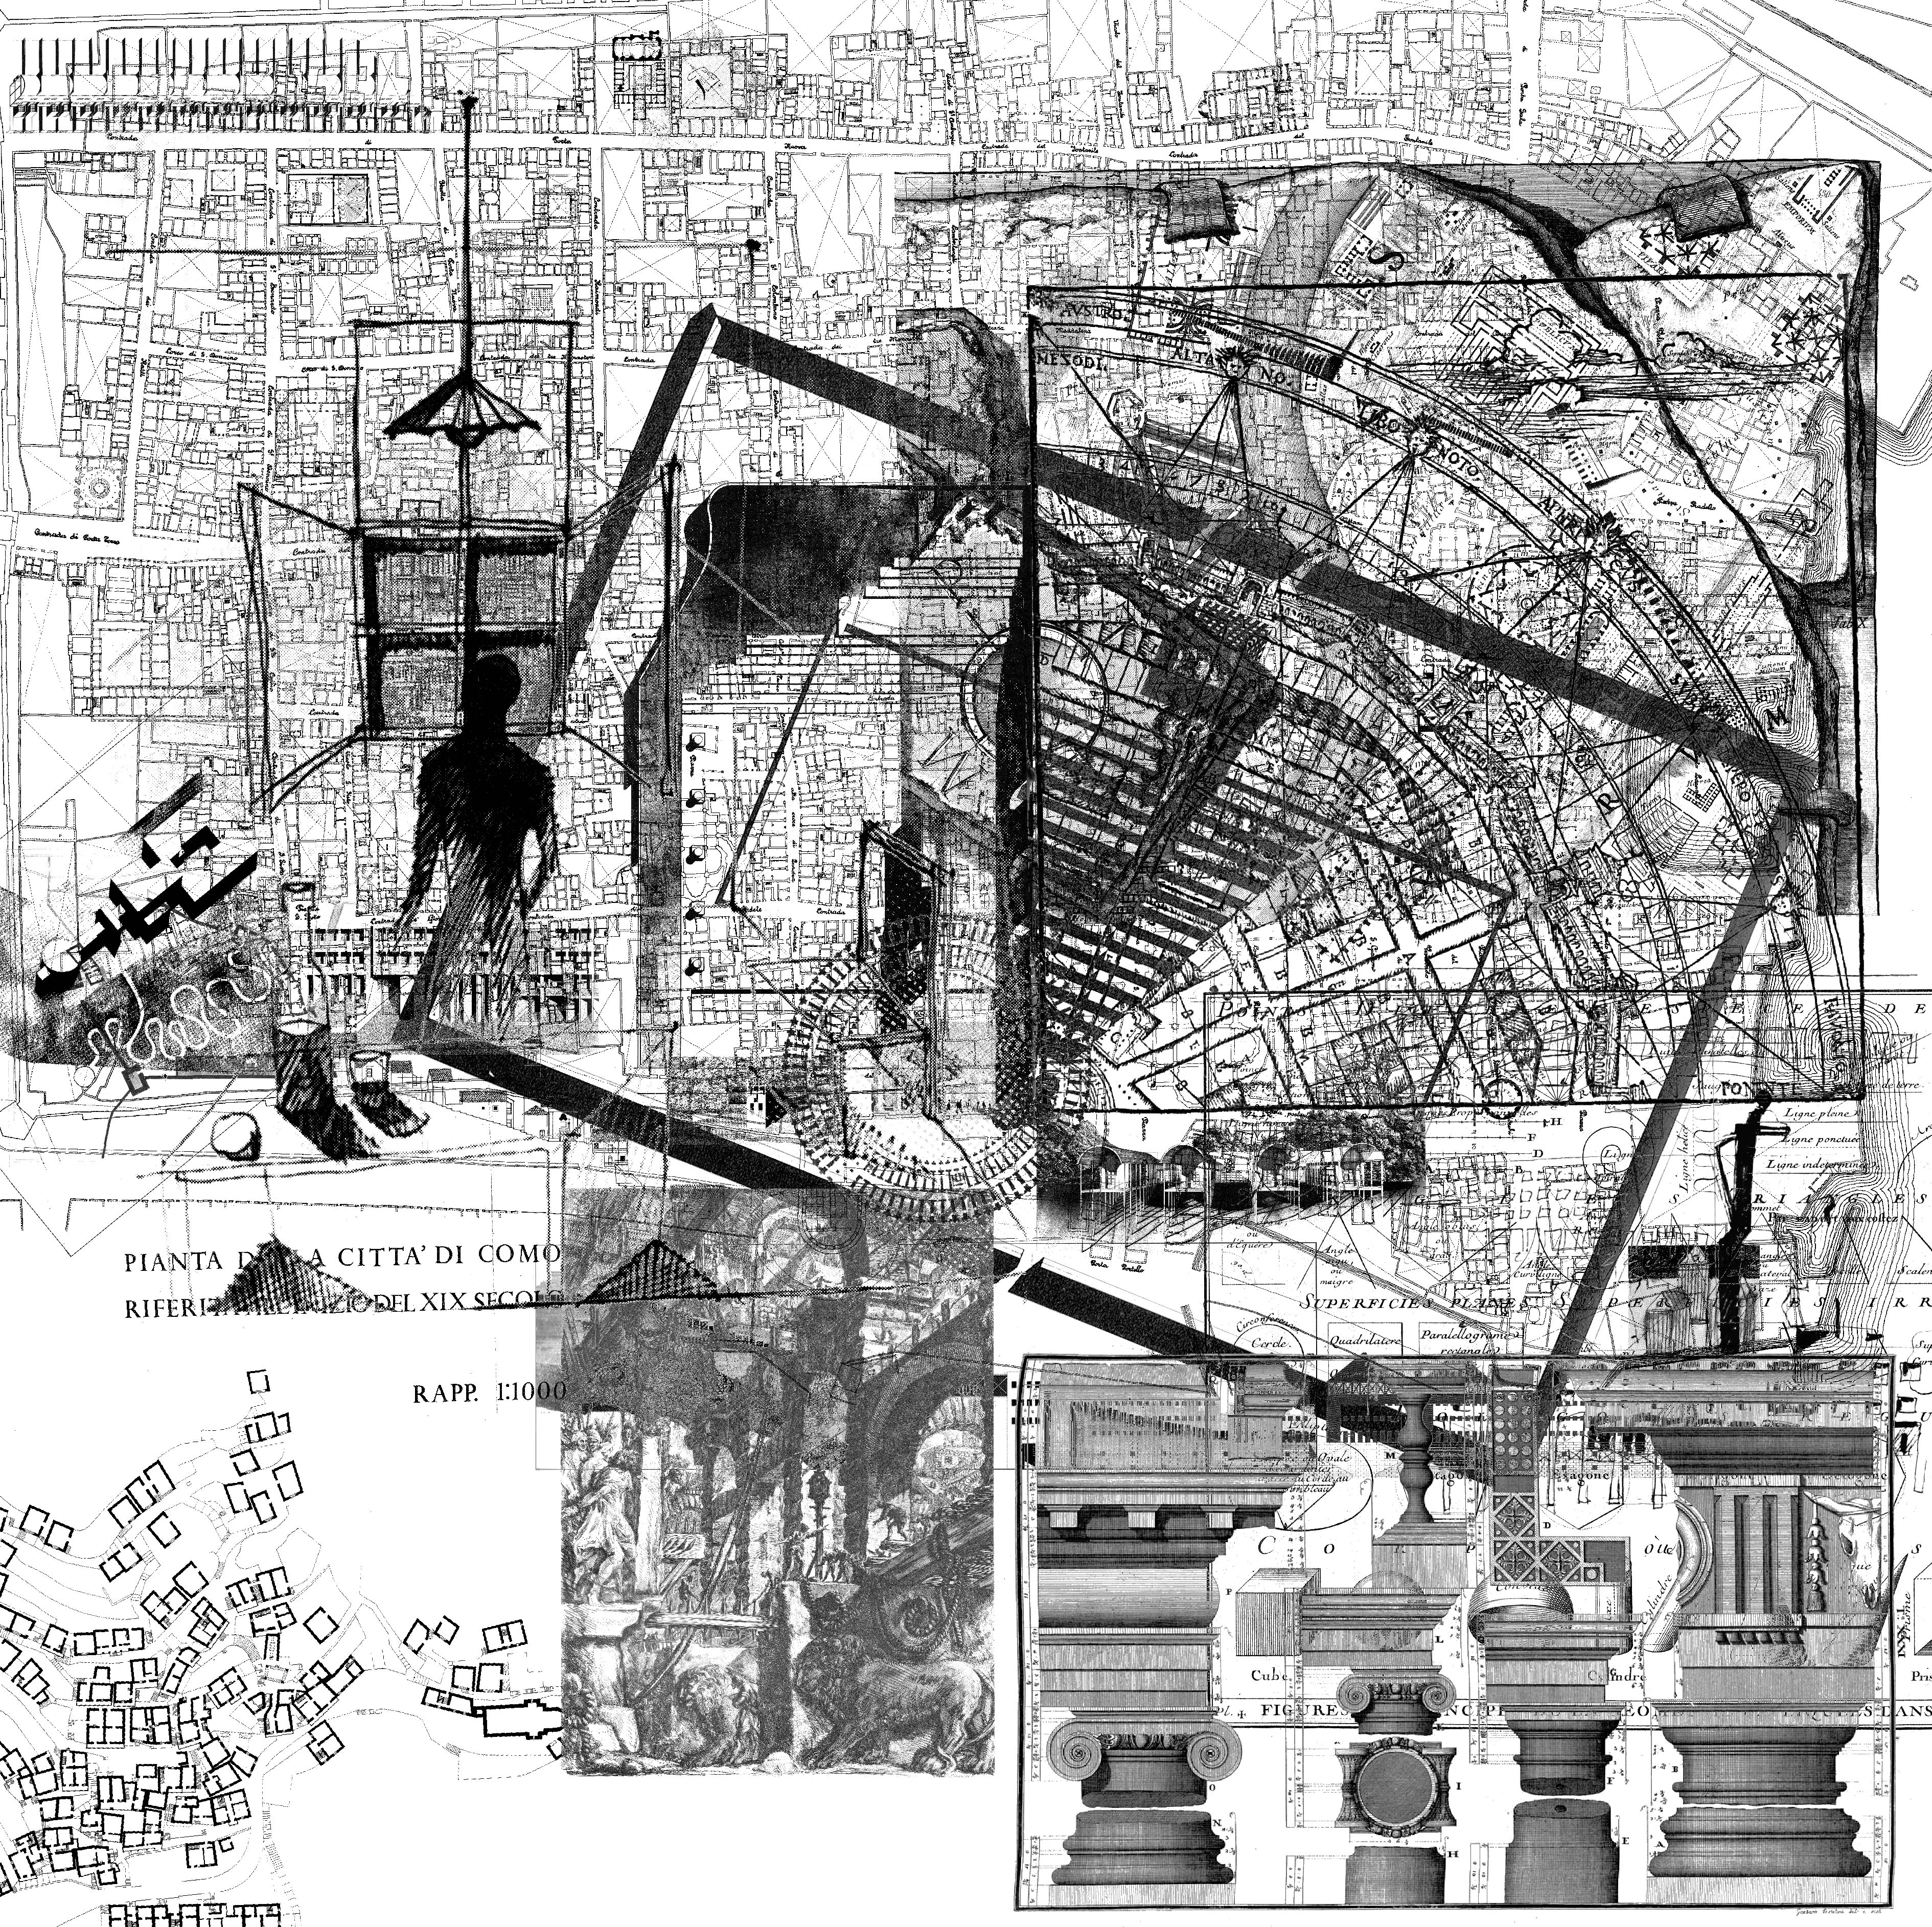
\includegraphics[width=0.85\linewidth]{analogous_city.jpg}
\caption{\textit{Analogous City} %MDPI: Please confirm whether the incomplete content in this figure affects scientific understanding and if it does, please revise it.
reinterpreted through digital analysis \cite{rodighiero_extending_2022}. First conceived as a collage for the Venice Biennale, the work has been studied as a critical artifact of architectural imagination \cite{ghirardo_aldo_2019, lampariello_aldo_2017}.}
\label{fig:analogous_city}
\end{figure}

Urban design provides the first anchors for this argument. Rossi’s \textit{Scientific Autobiography} describes architectural types as elements of reinvention, foregrounding how forms endure even as they shift in meaning and function \cite{rossi_scientific_1981}. A type is a structure that absorbs different uses across time, linking permanence with transformation. This line of thought resonates with the Italian school of urban morphology, from Saverio Muratori’s early work on typological processes \cite{muratori_studi_1963} to Gianfranco Caniggia and Gian Luigi Maffei’s systematization of building typologies as dynamic structures of continuity and change \cite{caniggia_composizione_1979}. Kevin Lynch’s \textit{The Image of the City} complements this perspective by showing how urban spaces are inscribed in collective memory through maps and mental images, revealing the accumulation of meaning \cite{lynch_image_1960}. For Lynch, legibility is a form of cognitive mapping that connects spatial form to lived experience, an idea later developed by Françoise Choay, who emphasized the cultural construction of historical environments \cite{choay_lallegorie_1992}. Peter Eisenman’s \textit{Diagram Diaries} extends these concerns into the computational register, conceiving diagrams as generative operators in the design process \cite{eisenman_peter_1999}. Here, diagrams function as representational devices of abstraction and recombination, allowing design to emerge through iterative sequences. Read together, these works suggest that urban form is stratified, layered, and continually reshaped by memory, imagination, and interpretation.

\textit{Actor--Network Theory} (ANT) adds a relational lens to this discussion. Emerging in the 1980s as a critique of deterministic models in science and technology studies, ANT emphasized that agency is distributed across networks of human and nonhuman actors \cite{akrich_sociologie_2006}. Latour’s essay \textit{Visualisation and Cognition} showed how maps are active mediators that make knowledge stable and transportable \cite{latour_visualisation_1986}. His later project \textit{Paris: Invisible City} extended this idea to the urban scale, tracing how infrastructures, technologies, and practices sustain city life through fragile alignments \cite{latour_paris_2021}. ANT thus resonates strongly with urban design: it makes visible how the city is continuously enacted through negotiations between people and infrastructures. Rather than treating urban form as the endpoint of planning, ANT recasts it as a choreography of associations, stabilized only through the everyday work of alignment. This perspective has been influential in urban studies and architecture, from Albena Yaneva’s ethnographies of architectural practice \cite{yaneva_mapping_2012} to Ignacio Farías’ work on urban assemblages \cite{farias_politics_2011} and Graham and Marvin’s account of infrastructural fragmentation \cite{graham_splintering_2001}. At the same time, ANT has faced criticism for flattening power relations and overemphasizing descriptive richness at the expense of normative critique, a limitation that must be acknowledged when adapting it to urban design. For urban studies, however, its enduring value lies in foregrounding the need to trace connections, mediations, and translations that bind together the visible and invisible dimensions of the built environment.

Information design provides the methodological resources to address these complexities. Manuel Lima’s \textit{Visual Complexity} surveys how networks make hidden structures perceptible across domains, offering inspiration for representing the entanglements that define urban assemblages \cite{lima_visual_2011}. Isabel Meirelles’ \textit{Design for Information} demonstrates how forms of visualization must be aligned with research questions, showing that design \mbox{decisions---choice} of diagram, scale, or metric---are integral to inquiry rather than secondary to it \cite{meirelles_design_2013}. Johanna Drucker’s \textit{Graphesis} emphasizes the interpretive nature of visualization, arguing that every graphical form carries rhetorical force and encodes specific ways of knowing~\cite{drucker_graphesis_2014}. This perspective has been reinforced by critical work in visualization studies, such as Lev Manovich’s notion of {cultural analytics \cite{manovich_cultural_2020}, which highlights how computational visualization reshapes the analysis of cultural and urban data, and Edward Tufte’s classic contributions on analytical design \cite{tufte_visual_2001}, which insist on clarity, minimalism, and evidence-based reasoning. Taken together, these works frame visualization as a theoretical practice that parallels the role of the diagram in architecture, as articulated by Eisenman \cite{eisenman_peter_1999}. Visualizations are not simply means of communication; they are engines of discovery and interpretation, structuring how we perceive relations, imagine alternatives, and contest meanings. For urban design, this suggests that computational visualization is a generative practice that actively shapes how urban form is conceptualized, debated, and~\mbox{transformed}.

% I REMOVED THE ITALICS FOR CULTURA ANLAYTICS: IT'S NOT A TITLE

Building on this literature, this article asks: How can network visualization methods be adapted to capture urban morphology as both enduring and relational, able to register permanence and transformation across time? What does a computational \mbox{workflow---combining} clustering, dimensionality reduction, and case-study \mbox{analysis---reveal} about the coexistence of types and associations in urban form, and how can it translate abstract relations into patterns that designers can work with? More broadly, how might these methods reshape design theory by integrating insights from complex systems and information visualization, making visible the fragile alignments, infrastructures, and negotiations that stabilize or transform cities? These questions position the city as a living system of interactions, suggesting that network visualization can act as a design instrument: a way of exploring, testing, and communicating how urban forms emerge from the entanglement of social, material, and computational dynamics.


%%%%%%%%%%%%%%%%%%%%%%%%%%%%%%%%%%%%%%%%%%%%%%%%%%%%%%%%%%%%%%%%%%%%%%%
%                                                                     %
%                          Section 3                                  %
%                      Design Methodology                             %
%                                                                     %
%%%%%%%%%%%%%%%%%%%%%%%%%%%%%%%%%%%%%%%%%%%%%%%%%%%%%%%%%%%%%%%%%%%%%%%

\section{Design Methodology}\label{sec3}

Network visualization provides a powerful lens through which the complexity of cities can be studied. Unlike Euclidean conceptions of space---as fixed, measurable, and \mbox{absolute---networks} render the world through relational configurations, aligning with the topological insights first formalized by Euler \cite{shields_cultural_2012}. Composed of nodes and edges, these diagrams allow us  {to tracing how a system operates}. In this sense, network visualization resonates with the perspective of  {Actor--Network Theory}: rather than privileging structure or function, both ANT and network visualization foreground association, movement, and emergence. While ethnographic prose unfolds these dynamics in narrative form, network diagrams condense them into visual arguments---hierarchies, flows, or decentralizations can be grasped at a glance. The position of nodes, their spatial proximity, and the topology of their connections become interpretive choices, making the diagram not only a representational device but also a methodological approach. In urban studies, where complexity and relationality are often acknowledged but rarely visualized beyond plans or maps, network visualization introduces a new grammar for representing heterogeneity and uncovering logics---such as centrality, clustering, or modularity---that operate across both social and spatial systems. Its appeal is therefore not merely technical but epistemological: it encourages us to think in terms of interactions rather than locations and of dynamic systems rather than static forms.

% I simplified the first sentence and remove the italics

Building on this potential, the present study adapts a taxonomy of network visualizations to explore urban morphology through an interdisciplinary lens. Originally intended to trace the evolution of network diagrams across fields, this classification distinguishes fifteen types \cite{lima_visual_2011}  {(pp.~158--201).}  %MDPI: We revised the ref citation format, please confirm. PEREFCT TO ME
To make it workable, the classification was reduced to a smaller set, with spherical visualizations excluded as their perspective is incompatible with the bird’s-eye city maps. The cities were first identified through an iterative process that began with comparing the taxonomy’s images with possible urban forms. ChatGPT-4o was employed as a heuristic tool to generate candidate cases whose topological patterns aligned with the classification; these suggestions were then critically assessed and refined. Final choices prioritized the clarity of morphological form rather than historical or cultural representativeness, with some cities deliberately retained as test cases to stress-test the workflow and reveal its limitations. Once the set of cities was established, they were grouped into three overarching categories---\textit{Archetypal}, \textit{Geometrical}, and \textit{Relational}. These groups do not replace traditional morphological analysis \cite{lynch_image_1960} but rather complement it by emphasizing structural affinities \cite{rodighiero_mapping_2021}. Grouping in this way highlights differences among urban forms while also revealing potential similarities between them, representing a methodological inversion: using visual grammars from data visualization to classify cities. This transposition of *network literacy* into urban studies offers a novel framework for reading urban form not only through historical categories---Renaissance, modernist, postmodern---but also through patterns of connection, circulation, and emergence.

\begin{itemize}
    \item {Archetypal} %MDPI: Please confirm if the bold formatting is necessary; if not, please remove it. The following highlights are the same.
 morphologies assemble configurations that express spatial ideals through strong centrality, axial symmetry, and symbolic order. They are historically rooted in representations of power, divinity, or strategic control, projecting authority through coherence and legibility. Cities such as Rome, Vatican City, Fez, and Moscow exemplify this group (Table~\ref{table_archetypal}).  

    \item {Geometrical} morphologies rely on abstraction, symmetry, and repetition to structure the urban fabric. Emerging from planning logics that prioritize regularity---grids, radial divisions, and compositional order---they reflect rational planning and systematic articulation of space. Cities such as Medellín, Palmanova, Dubai, and Canberra illustrate this group (Table~\ref{table_geometrical}).  

    \item {Relational} morphologies emerge from flows, interactions, and negotiated proximities rather than fixed geometries or symbolic centers. They are layered, adaptive, and shaped by movement and accumulation, privileging connectivity and adjacency over hierarchy and alignment. Cities such as Los Angeles, Berlin, Cairo, and Amsterdam represent this group (Table~\ref{table_relational}).  
\end{itemize}

% I REMOVED THE BOLD

{The} %MDPI: We revised it to normal pragraph format with indent, please confirm.
city maps were generated with \textit{OSMnx}, an open-source  {Python} %MDPI: Please state which version of the software was used.
 library for modeling and analyzing urban form from OpenStreetMap data \cite{boeing_modeling_2025}. The library extracts nodes and edges by interpreting OpenStreetMap’s definitions of “streets” and “intersections,” a process that is not neutral: it reflects assumptions about what constitutes a valid topological element and how these should be abstracted into graph form. In this sense, the datasets embody both technical conventions and cultural decisions about the representation of urban space. Once imported, networks were stored and handled as graph objects, with intersections as nodes and street segments as edges. This representation provided a systematic basis for comparing cities across divergent contexts while retaining a common analytic language. At the same time, it foregrounded how infrastructural and cultural choices shape data: what is captured as a street or junction, what is omitted, and how such abstractions condition subsequent analyses. \textit{OSMnx} thus offered not only a practical tool for data collection and processing but also an opportunity to reflect critically on how digital infrastructures codify urban morphology.

 % Again, I am using a long list of libraries that are specified in the GitHib repository; there is no need to cite versions here—it's not relevant.

To analyze these networks, we used a computational pipeline that translates the complex web of streets and intersections into a form where patterns can be more easily studied. The first step employed \textit{Node2Vec} \cite{grover_node2vec_2016}, an algorithm that generates embeddings---numerical representations that capture how each node is positioned within both its immediate surroundings and the larger network. This is performed by simulating many short walks through the graph, recording how nodes are encountered together. To ensure comparability across all cases, we fixed the main parameters as follows:  \texttt{walk\_length}  %MDPI: Please check if the font should be kept.
= 80, \texttt{num\_walks} = 10, \texttt{dimensions} = 128, with return/in--out parameters $p = 1$ and $q = 1$ to balance attention between local neighborhoods and more distant routes. Because the resulting 128-dimensional vectors cannot be interpreted directly, we applied \textit{UMAP} \cite{mcinnes_umap_2018}, a dimensionality reduction technique that preserves neighborhood relations while compressing the data into a two-dimensional space suitable for visualization. Here, we used \texttt{n\_neighbors} = 15, \mbox{\texttt{min\_dist} = 0.1}, and an output dimensionality of 2. The resulting diagrams place structurally similar intersections close together, allowing meaningful spatial patterns to emerge. To move from visualization to systematic grouping, we then applied \textit{HDBSCAN} \cite{mcinnes_hdbscan_2017}, a clustering algorithm well suited to complex data, with parameters \mbox{\texttt{min\_cluster\_size} = 30} and \mbox{\texttt{min\_samples} = 10.} This balance allowed the detection of fine-grained clusters. Together, these steps translated urban networks into forms that reveal robust structural patterns across different cities.

The results were visualized by pairing UMAP-colored embeddings with geographic city maps, assigning consistent colors across both to make structural features comparable under two different spatializations. This juxtaposition highlights how computational reductions and cartographic representations reveal complementary perspectives on the same urban fabric---one emphasizing structural affinities, the other geographic placement. To ensure transparency and facilitate reuse, the complete workflow is openly available in the  {GitHub} %MDPI: Please state which version of the software was used.
 repository, along with software library versions \cite{rodighiero_urban-mapper_2025}.

 % I SPECIFIED HERE WHERE THE SOFTAWRE VERISON ARE AVAILABLE

%%%%%%%%%%%%%%%%%%%%%%%%%%%%%%%%%%%%%%%%%%%%%%%%%%%%%%%%%%%%%%%%%%%%%%%
%                        Info - Taxonomy - Maps                       %
%%%%%%%%%%%%%%%%%%%%%%%%%%%%%%%%%%%%%%%%%%%%%%%%%%%%%%%%%%%%%%%%%%%%%%%

\begin{table}[H]
\caption{{Archetypal}  %MDPI: We added border lines in the table to make it look better, please confirm. Tables below are the same.
group of cities considered in this study: Rome (Italy), Vatican City (Vatican), Fez (Morocco), and Moscow (Russia). For each city, the table provides basic data, the black-and-white map projection at the chosen scale, and the corresponding taxonomy icon from Lima’s classification.}
\label{table_archetypal}

% IT'S BEAUTIFUL, THANK YOU!


\begin{adjustwidth}{-\extralength}{0cm}
%\centering %% If there is a figure in wide page, please release command \centering
\begin{tabularx}{\fulllength}{>{\raggedright\arraybackslash}Xm{6cm}<{\centering}m{6cm}<{\centering}}
\toprule
\textbf{City} & \textbf{Taxonomy} & \multicolumn{1}{c}{\textbf{Map}} \\
\midrule
\textbf{{Rome}} \newline Country: Italy \newline Lat/Lon: (41.8941, 12.4856) \newline Scale: 10 km \newline Group: Archetypal \newline Taxonomy Label: \newline Radial Implosion &
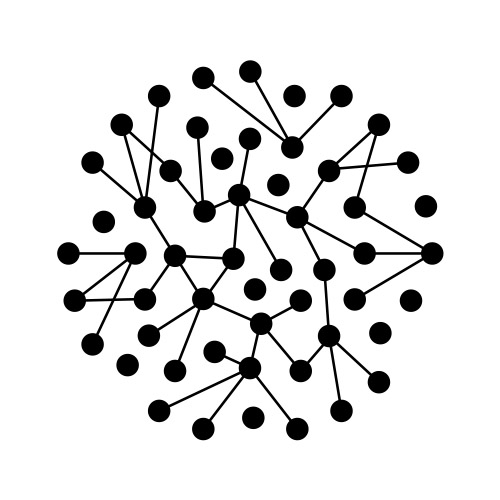
\includegraphics[width=0.88\linewidth]{taxonomy/Radial_Implosion.jpg} &

\includegraphics[width=0.88\linewidth]{maps_b&w/Rome.png} \\[-2ex]
\midrule
\textbf{{Vatican City}} \newline Country: Vatican \newline Lat/Lon: (41.9023, 12.4574) \newline Scale: 1 km \newline Group: Archetypal \newline Taxonomy Label: \newline Elliptical Implosion &
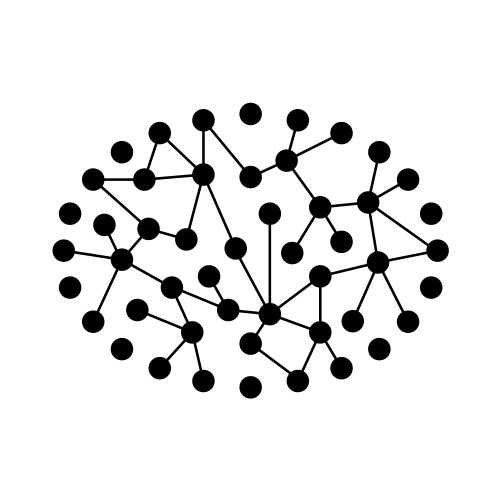
\includegraphics[width=0.88\linewidth]{taxonomy/Elliptical_Implosion.jpg} &

\includegraphics[width=0.88\linewidth]{maps_b&w/Vatican_City.png} \\[-0.8ex]
\midrule
\textbf{{Fez}} \newline Country: Morocco \newline Lat/Lon: (34.0650, $-$4.9730) \newline Scale: 1 km \newline Group: Archetypal \newline Taxonomy Label: \newline Organic Rhizome &
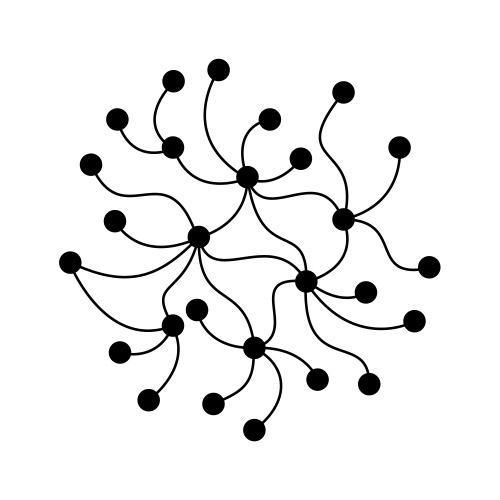
\includegraphics[width=0.88\linewidth]{taxonomy/Organic_Rhizome.jpg} &

\includegraphics[width=0.88\linewidth]{maps_b&w/Fez.png} \\[-0.5ex]
\midrule
\textbf{{Moscow}} \newline Country: Russia \newline Lat/Lon: (55.7558, 37.6176) \newline Scale: 5 km \newline Group: Archetypal \newline Taxonomy Label: \newline Centralized Burst &
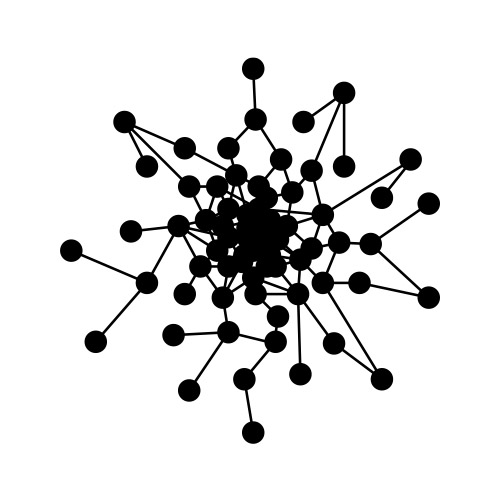
\includegraphics[width=0.88\linewidth]{taxonomy/Centralized_Burst.jpg} &

\includegraphics[width=0.88\linewidth]{maps_b&w/Moscow.png} \\[-0.8ex]
\bottomrule
\end{tabularx}
\end{adjustwidth}

\end{table}

\begin{table}[H]
\caption{Geometrical group of cities considered in this study: Medellin (Colombia), Palmanova (Italy), Dubai (UAE), and Canberra (Australia). For each city, the table provides basic data, the black-and-white map projection at the chosen scale, and the corresponding taxonomy icon from Lima’s classification.}
\label{table_geometrical}

\begin{adjustwidth}{-\extralength}{0cm}
%\centering %% If there is a figure in wide page, please release command \centering
\begin{tabularx}{\fulllength}{>{\raggedright\arraybackslash}X m{6cm}<{\centering}m{6cm}<{\centering}}
\toprule
\textbf{City} & \multicolumn{1}{c}{\textbf{Taxonomy}} & \multicolumn{1}{c}{\textbf{Map}} \\
\midrule
\textbf{{Medellin}} \newline Country: Colombia \newline Lat/Lon: (6.2518, $-$75.5836) \newline Scale: 10 km \newline Group: Geometrical \newline Taxonomy Label: \newline Arc Diagram &
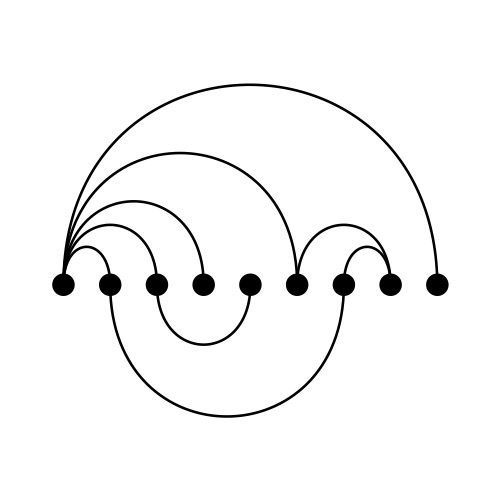
\includegraphics[width=0.85\linewidth]{taxonomy/Arc_Diagram.jpg} &

\includegraphics[width=0.85\linewidth]{maps_b&w/Medellin.png} \\[-3ex]
\midrule
\textbf{{Palmanova}} \newline Country: Italy \newline Lat/Lon: (45.9061, 13.3095) \newline Scale: 1 km \newline Group: Geometrical \newline Taxonomy Label: \newline Radial Convergence &
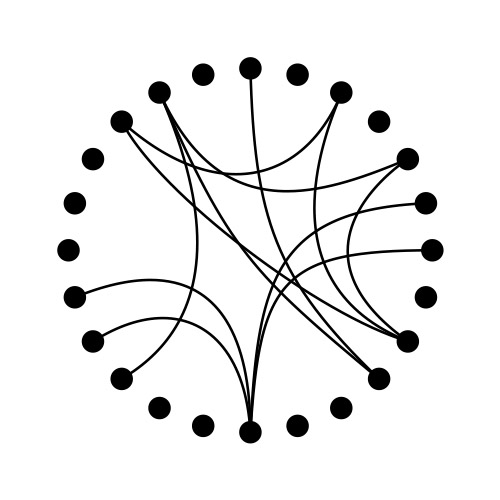
\includegraphics[width=0.85\linewidth]{taxonomy/Radial_Convergence.jpg} &

\includegraphics[width=0.85\linewidth]{maps_b&w/Palmanova.png} \\[-0.5ex]
\midrule
\textbf{{Dubai}} \newline Country: United Arab Emirates \newline Lat/Lon: (25.0565, 55.2070) \newline Scale: 1 km \newline Group: Geometrical \newline Taxonomy Label: \newline Segmented Radial Convergence &
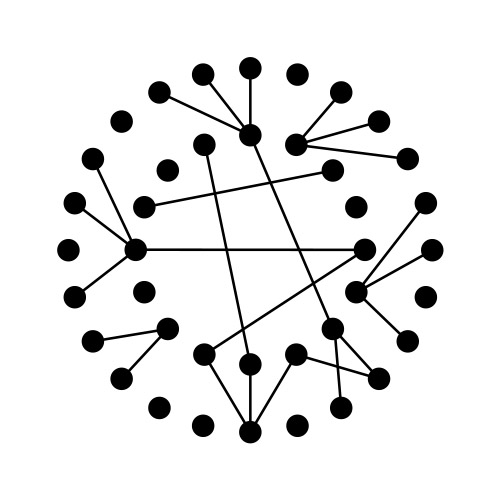
\includegraphics[width=0.85\linewidth]{taxonomy/Segmented_Radial_Convergence.jpg} &

\includegraphics[width=0.85\linewidth]{maps_b&w/Dubai.png} \\[-0.5ex]
\midrule
\textbf{{Canberra}} \newline Country: Australia \newline Lat/Lon: ($-$35.3082, 149.1244) \newline Scale: 3.5 km \newline Group: Geometrical \newline Taxonomy Label: \newline Centralized Ring &
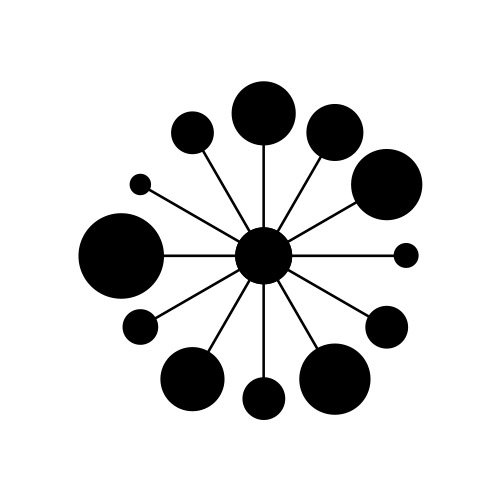
\includegraphics[width=0.85\linewidth]{taxonomy/Centralized_Ring.jpg} &

\includegraphics[width=0.85\linewidth]{maps_b&w/Canberra.png} \\[-0.5ex]
\bottomrule
\end{tabularx}
\end{adjustwidth}
\end{table}

\begin{table}[H]
\caption{Relational group of cities considered in this study: Los Angeles (USA), Berlin (Germany), Cairo (Egypt), and Amsterdam (Netherlands). For each city, the table provides basic data, the black-and-white map projection at the chosen scale, and the corresponding taxonomy icon from Lima’s~\mbox{classification}.}
\label{table_relational}

\begin{adjustwidth}{-\extralength}{0cm}
%\centering %% If there is a figure in wide page, please release command \centering
\begin{tabularx}{\fulllength}{>{\raggedright\arraybackslash}X m{6cm}<{\centering}m{6cm}<{\centering}}
\toprule
\textbf{City} & \multicolumn{1}{c}{\textbf{Taxonomy}} & \multicolumn{1}{c}{\textbf{Map}} \\
\midrule
\textbf{{Los Angeles}} \newline Country: United States \newline Lat/Lon: (34.0293, $-$118.2144) \newline Scale: 1 km \newline Group: Relational \newline Taxonomy Label: \newline Flow Chart &

\includegraphics[width=0.9\linewidth]{taxonomy/Flow_Chart.jpg} &

\includegraphics[width=0.9\linewidth]{maps_b&w/Los_Angeles.png} \\[-2.5ex]
\midrule
\textbf{{Berlin}} \newline Country: Germany \newline Lat/Lon: (52.5200, 13.4050) \newline Scale: 5 km \newline Group: Relational \newline Taxonomy Label: \newline Area Grouping &
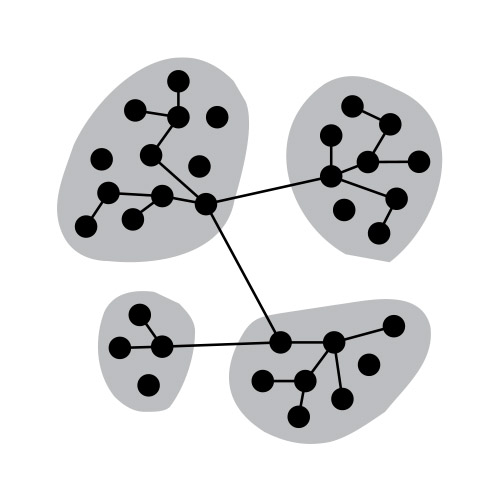
\includegraphics[width=0.9\linewidth]{taxonomy/Area_Grouping.jpg} &

\includegraphics[width=0.9\linewidth]{maps_b&w/Berlin.png} \\[-1.5ex]
\midrule
\textbf{{Cairo}} \newline Country: Egypt \newline Lat/Lon: (30.0444, 31.2357) \newline Scale: 5 km \newline Group: Relational \newline Taxonomy Label: \newline Circular Ties &
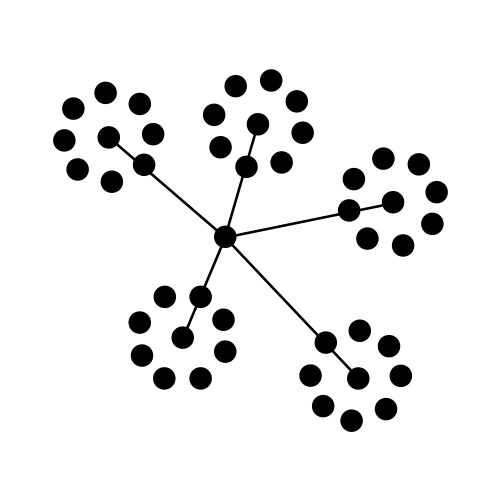
\includegraphics[width=0.9\linewidth]{taxonomy/Circular_Ties.jpg} &

\includegraphics[width=0.9\linewidth]{maps_b&w/Cairo.png} \\[-0.5ex]
\midrule
\textbf{{Amsterdam}} \newline Country: Netherlands \newline Lat/Lon: (52.3710, 4.9000) \newline Scale: 2 km \newline Group: Relational \newline Taxonomy Label: \newline Ramification &
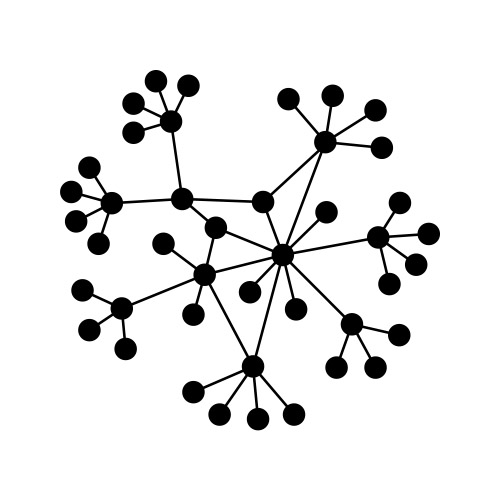
\includegraphics[width=0.9\linewidth]{taxonomy/Ramification.jpg} &

\includegraphics[width=0.9\linewidth]{maps_b&w/Amsterdam.png} \\[-0.5ex]
\bottomrule
\end{tabularx}
\end{adjustwidth}
\end{table}



%%%%%%%%%%%%%%%%%%%%%%%%%%%%%%%%%%%%%%%%%%%%%%%%%%%%%%%%%%%%%%%%%%%%%%%
%                                                                     %
%                          Section 4                                  %
%                   Interpretative Results                            %
%                                                                     %
%%%%%%%%%%%%%%%%%%%%%%%%%%%%%%%%%%%%%%%%%%%%%%%%%%%%%%%%%%%%%%%%%%%%%%%

\section{Interpretative Results}\label{sec4}

The interpretative power of this methodology lies in the dialogue between embeddings and maps. The consistent use of colors across both representations enables a scalable operation: one begins by linking a cluster in the map with its equivalent in the embedding, then gradually extends this comparison to adjacent clusters, reconstructing a correspondence between the two spatializations. This back-and-forth movement makes visible both alignments and divergences between cartographic form and topological reduction. To frame these results, the cities have been organized into three morphological groups---{Archetypal}, {Geometrical}, and {Relational}---summarized in Tables~\ref{table_archetypal_embeddings}--\ref{table_relational_embeddings}. The following discussion highlights one emblematic case from each group.

% I REMIVE ITALICS HERE

The {Archetypal} group (Table~\ref{table_archetypal_embeddings}) underscores the importance of scale. Compact entities such as Vatican City and Fez emerge in embeddings as tightly woven and legible, where different neighborhoods are clearly distinguished at a small scale. In these cases, the embedding highlights the density and coherence of historical fabrics, where layered morphologies can still be untangled into identifiable clusters. By contrast, large metropolitan contexts like Moscow posed a particular challenge. The initial idea was to work at a scale of 50 km, considering the immense size of the capital, but the results were not appreciable. The scale was therefore reduced to 10 km, where the embedding performs somewhat better, though still without reaching the clarity observed in smaller cities. These cases show how scale determines whether topological reduction can yield interpretable results, emphasizing the fragility of embeddings when cities become too expansive.

Expanding the view from Vatican City gives the full picture of Rome, where the embedding reveals the city’s fragmented morphology (Figure~\ref{rome}). Rather than a unified fabric, Rome appears as a patchwork of absorbed villages, structured by the \textit{{Grande Raccordo Anulare}} (GRA), the orbital motorway encircling the capital. Conceived in the late 1940s and completed in stages by the 1970s, the GRA was not only a transportation infrastructure but also a political instrument framing the city’s limits. This dual role has been poignantly portrayed in Gianfranco Rosi’s documentary \textit{{Sacro GRA}} \cite{rosi_sacro_2013}, which explores the lives unfolding along the motorway’s edge. The embedding captures this dispersed aggregation, contrasting it with Vatican City’s compact coherence, and demonstrates how infrastructural borders such as the GRA shape the city’s topological order.

\vspace{-8pt}
\begin{figure}[H]
\hspace{-7mm}
\begin{minipage}[t]{0.49\textwidth}
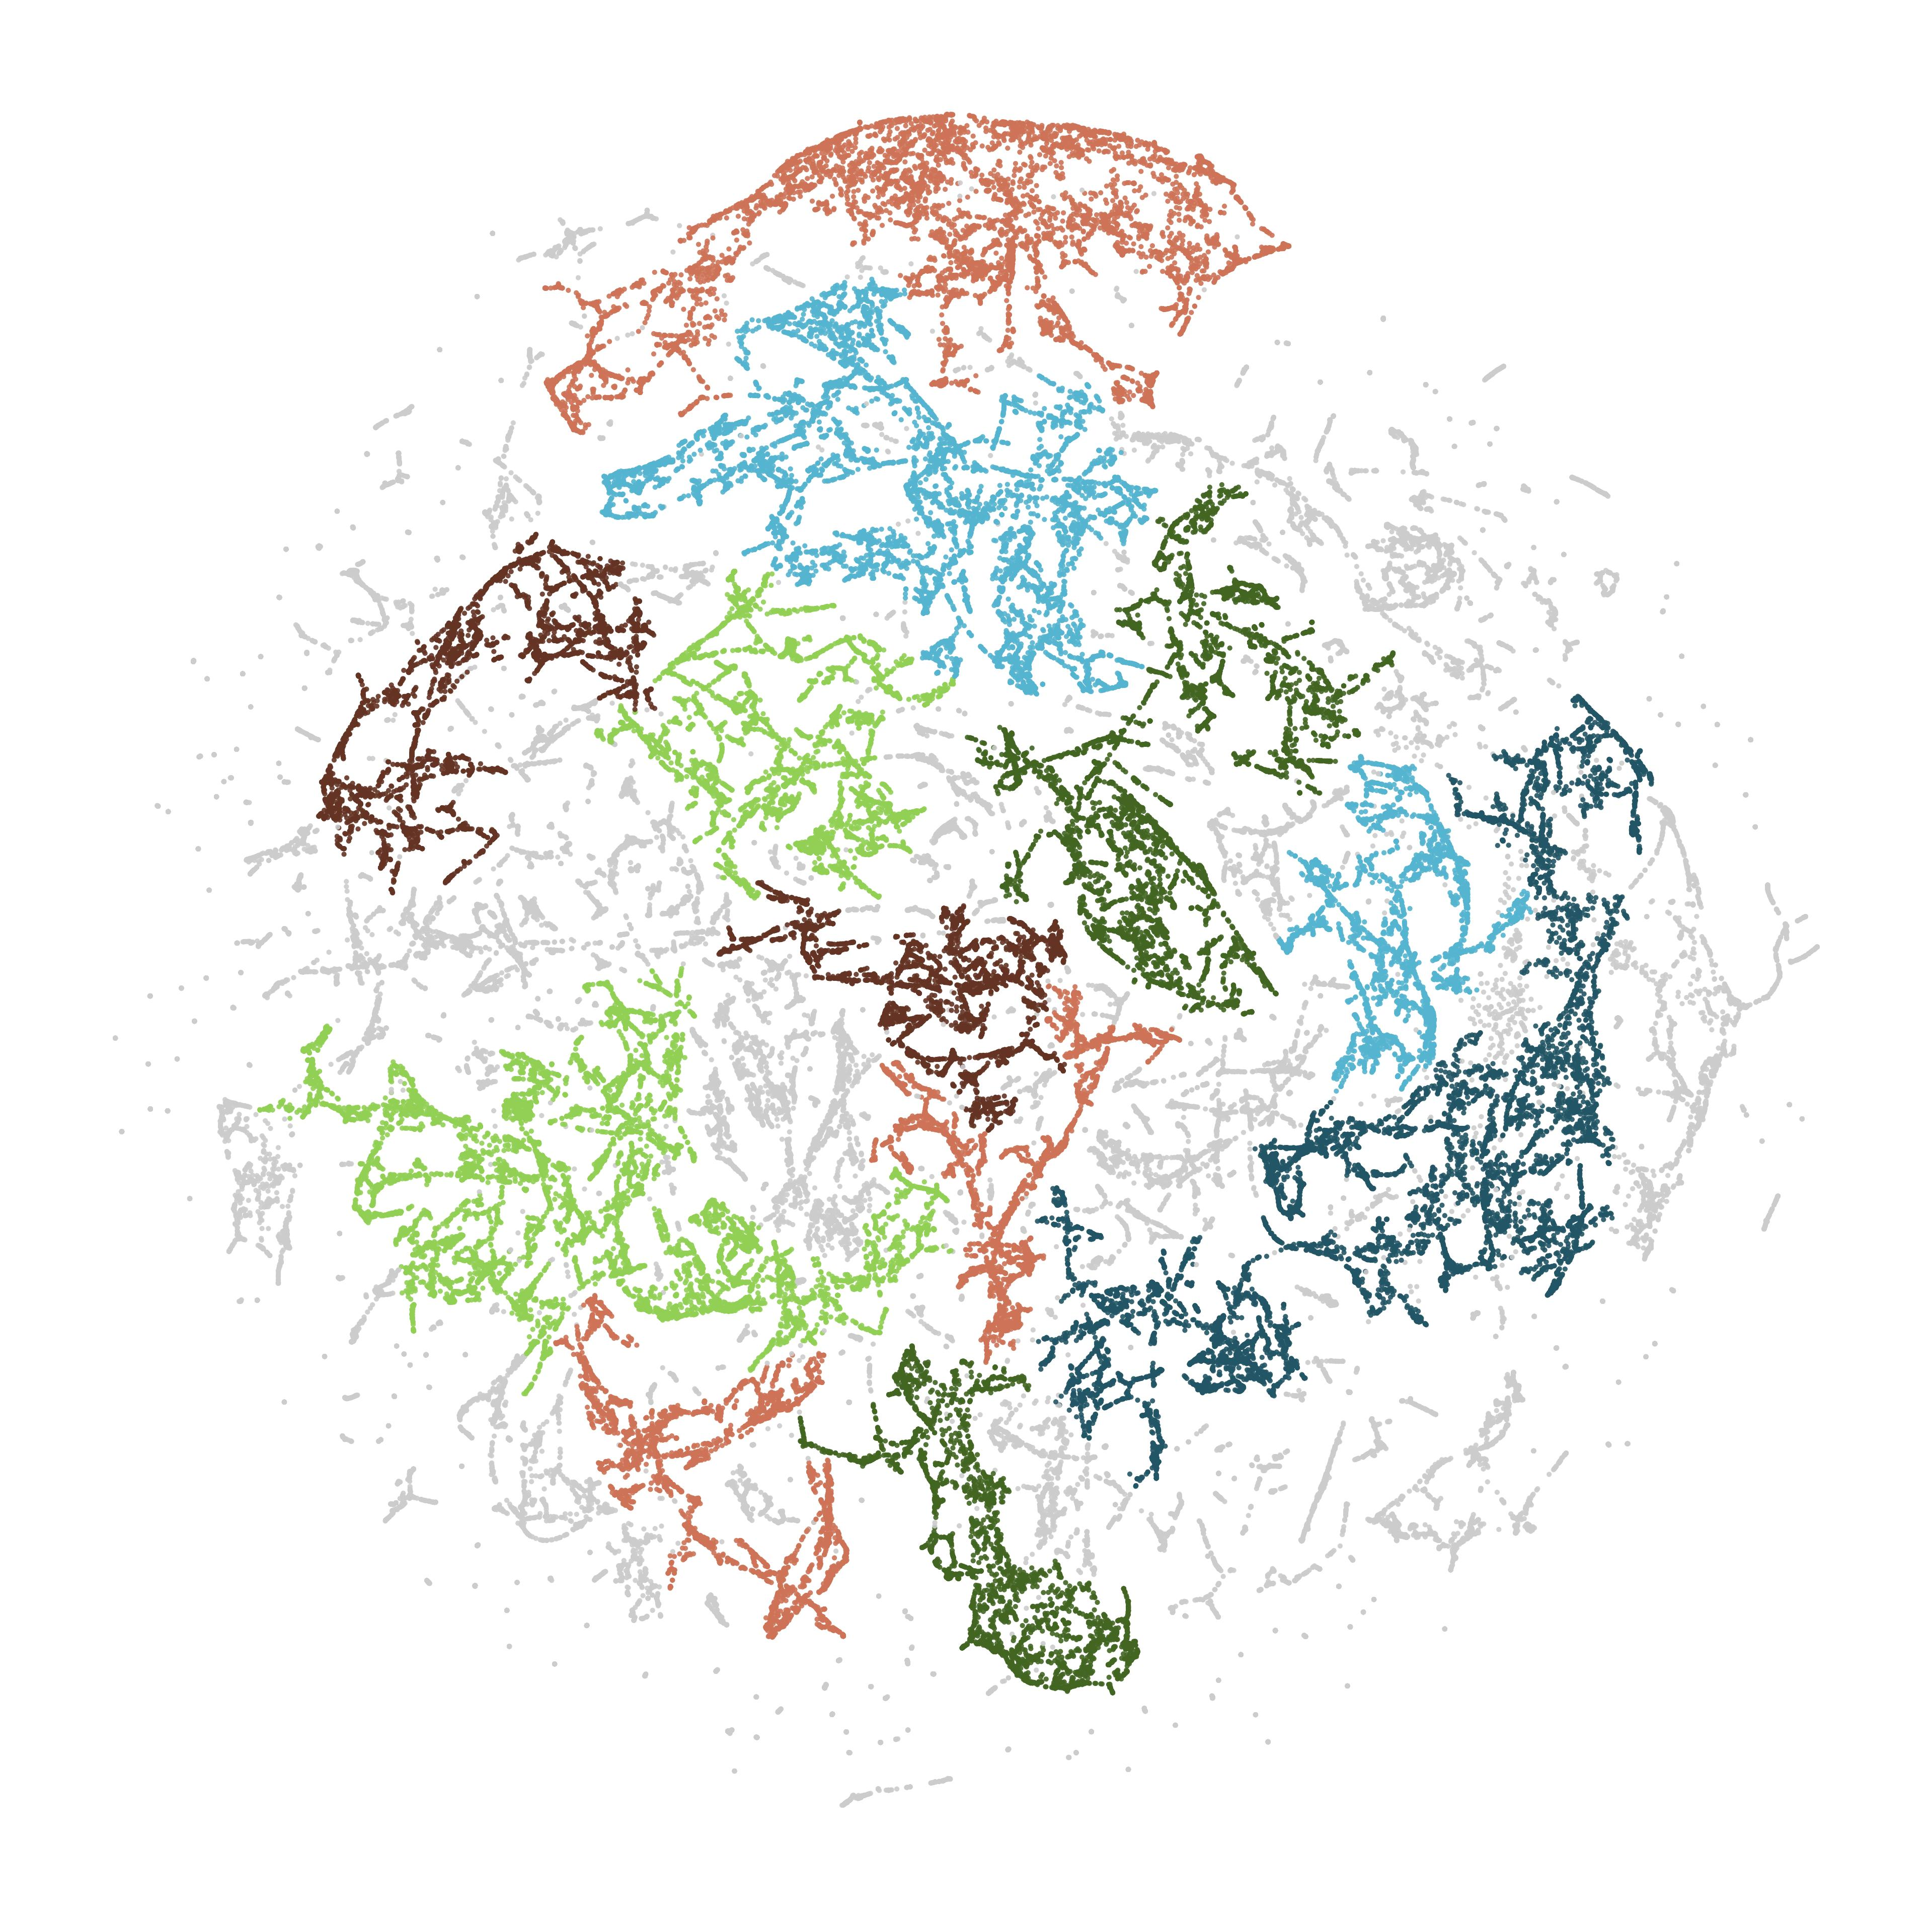
\includegraphics[width=\linewidth]{clusters/Rome.jpg}
\end{minipage}\hfill
\begin{minipage}[t]{0.49\textwidth}
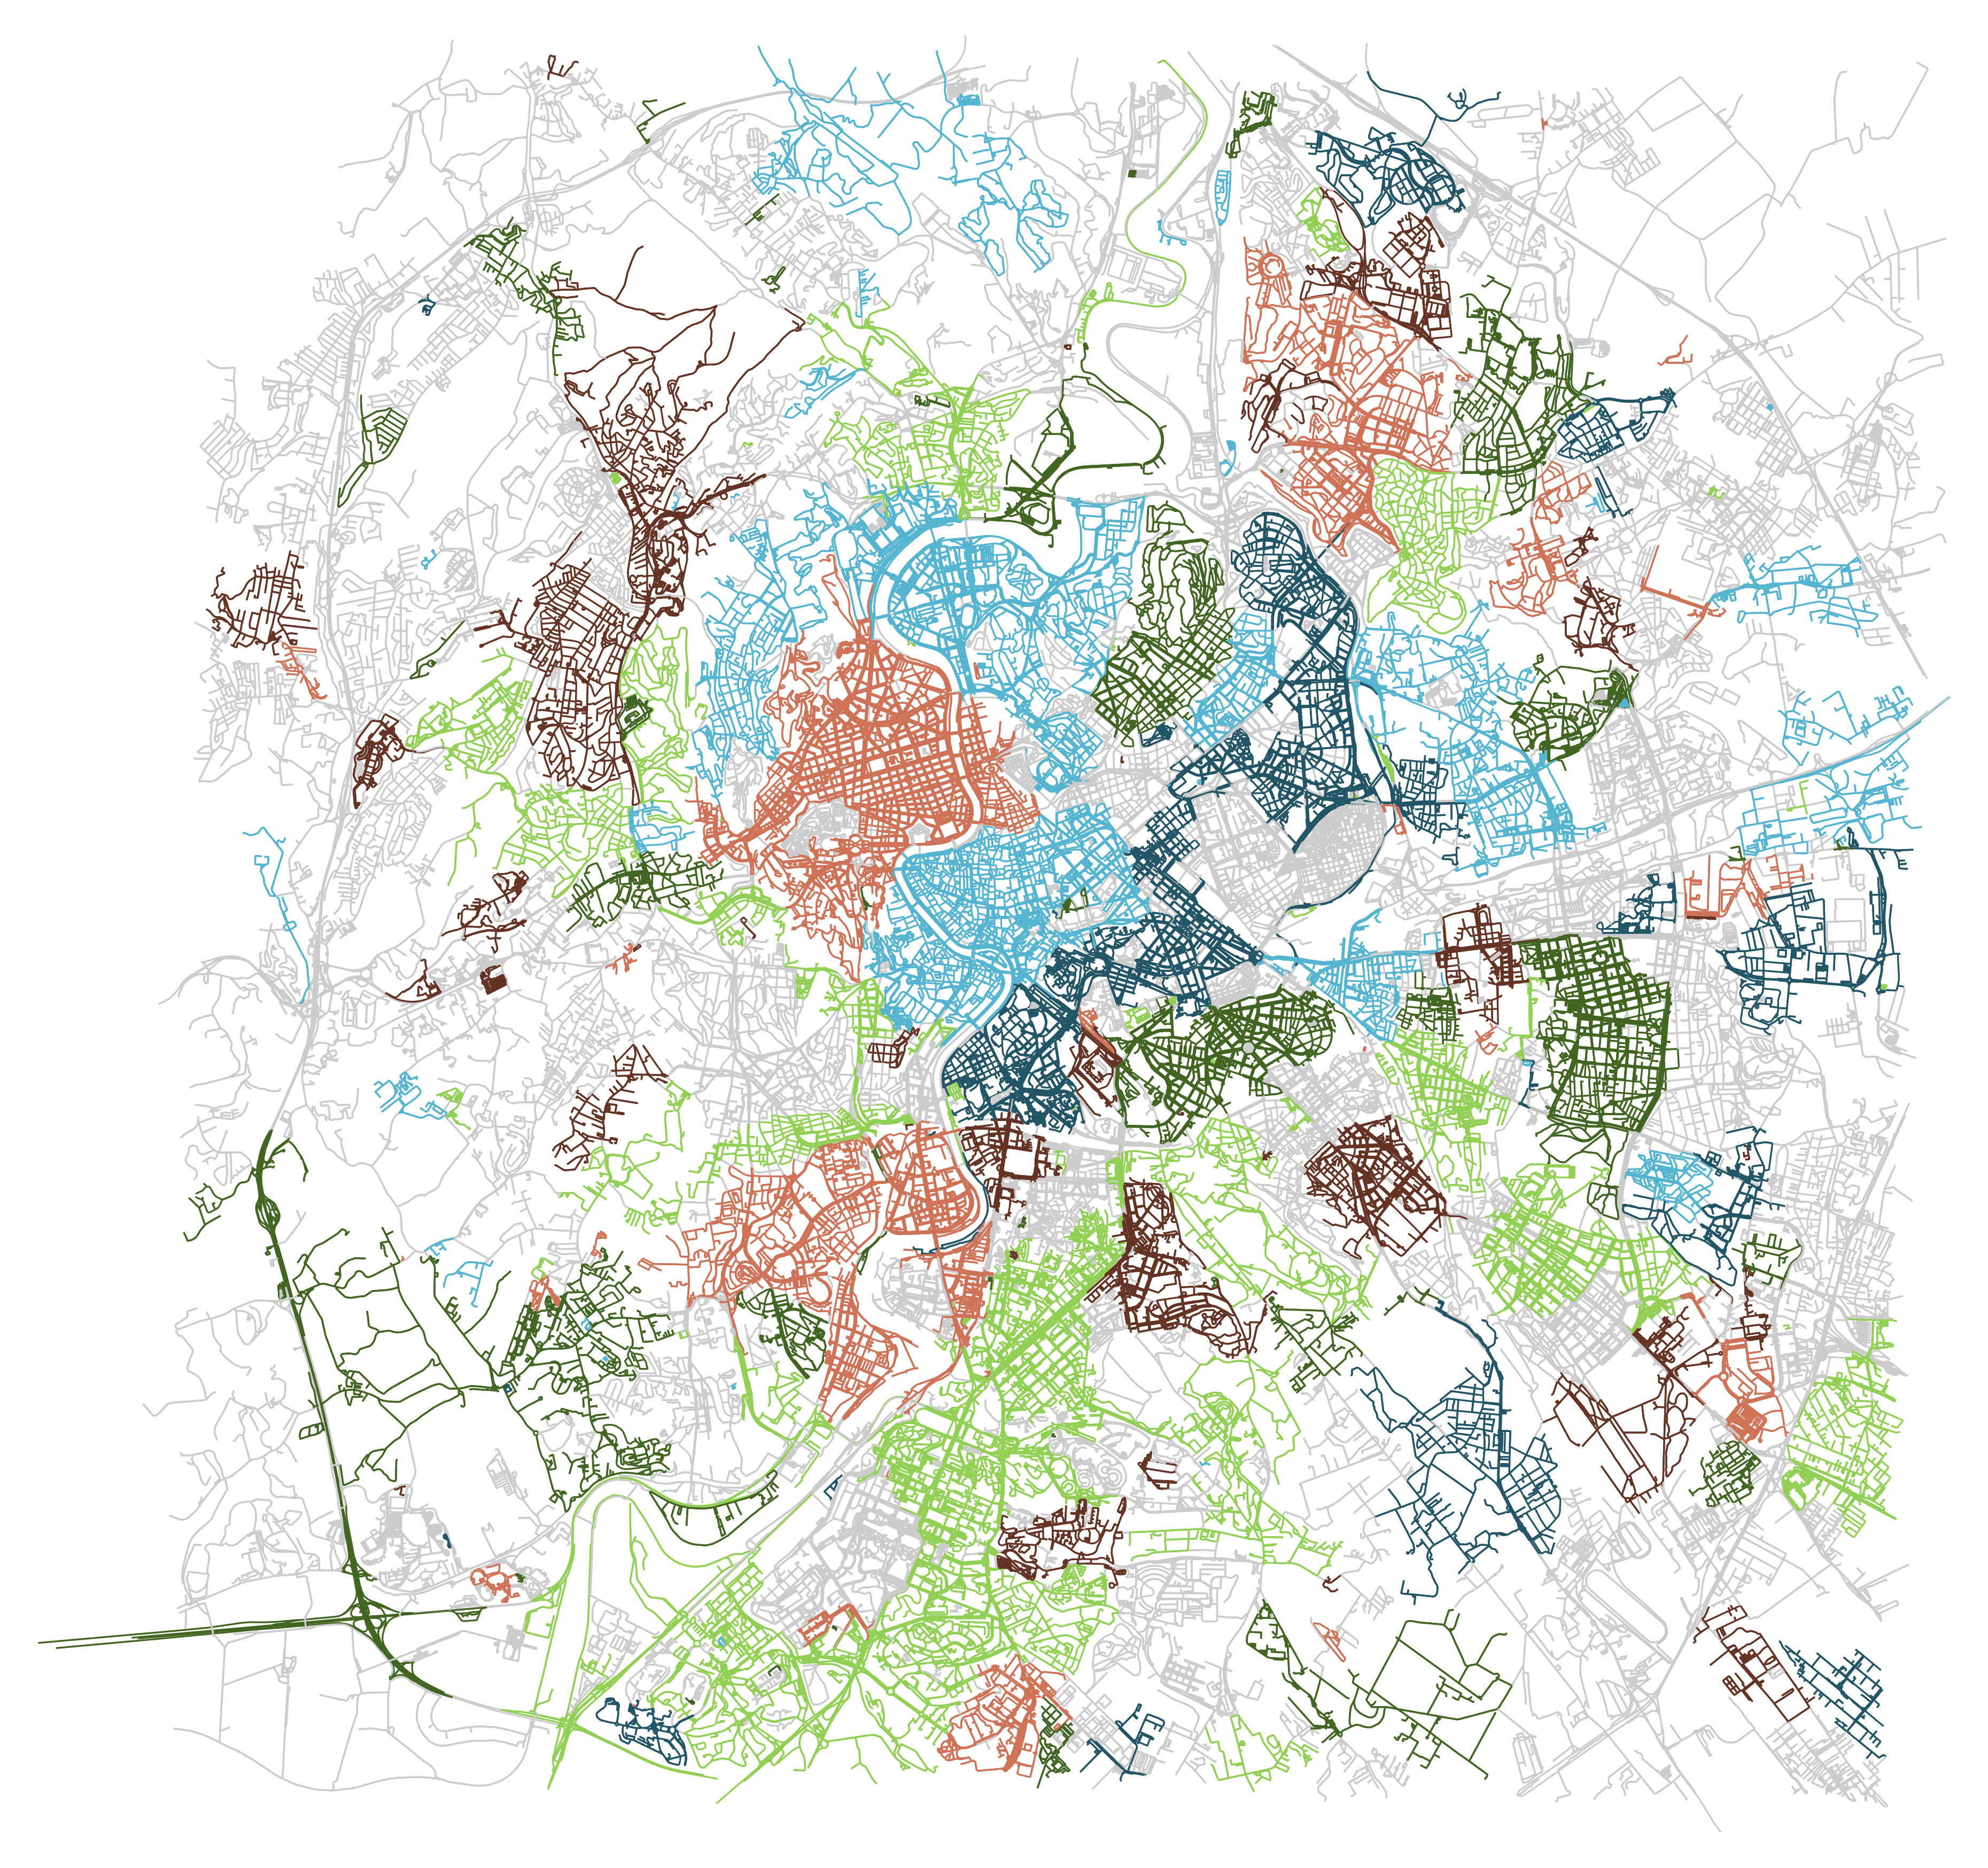
\includegraphics[width=\linewidth]{maps/Rome.png}
\end{minipage}
\caption{{Rome.} %MDPI: Please check if there should add an explanation for colors in the figure. if yes, please add. Figures 3-5 are the same.
 The embedding reveals the scattered distribution of neighborhoods unified by the \textit{{Grande Raccordo Anulare}}, contrasting with the compactness of Vatican City. The result highlights Rome’s character as a patchwork of absorbed villages held together by infrastructure.}
\label{rome}
\end{figure}

% IT'S FINE AS IT IS, THANKS

The {Geometrical} group (Table~\ref{table_geometrical_embeddings}) reveals a tension between confirmation and loss of intended design. Palmanova’s Renaissance plan, for instance, loses clarity in the embedding, its radial order blurred into indistinct clusters. Medellín, structured along valleys and linear corridors, similarly dissolves, its cartographic legibility not surviving translation into topological space. These cases show how geometry can either endure or collapse, depending on the rigidity of its urban plan.

Among the more resilient examples are Dubai and Canberra. Dubai retains its hexagonal slices with striking fidelity (Figure~\ref{fig:dubai}); even the subdivision of individual sectors appears in the embedding, reflecting the rationalized planning and infrastructural hierarchies that reinforce its geometric order. Canberra, by contrast, weakens in overall radial and axial clarity (Figure~\ref{fig:canberra}), yet its neighborhoods remain coherent and legible enough to echo the city’s planned design. Together, these cases illustrate how certain planned morphologies can preserve topological coherence, while others partially dissolve yet still maintain recognizable structures.

\vspace{-4pt}
\begin{figure}[H]
\hspace{-3mm}
\begin{minipage}[t]{0.49\textwidth}
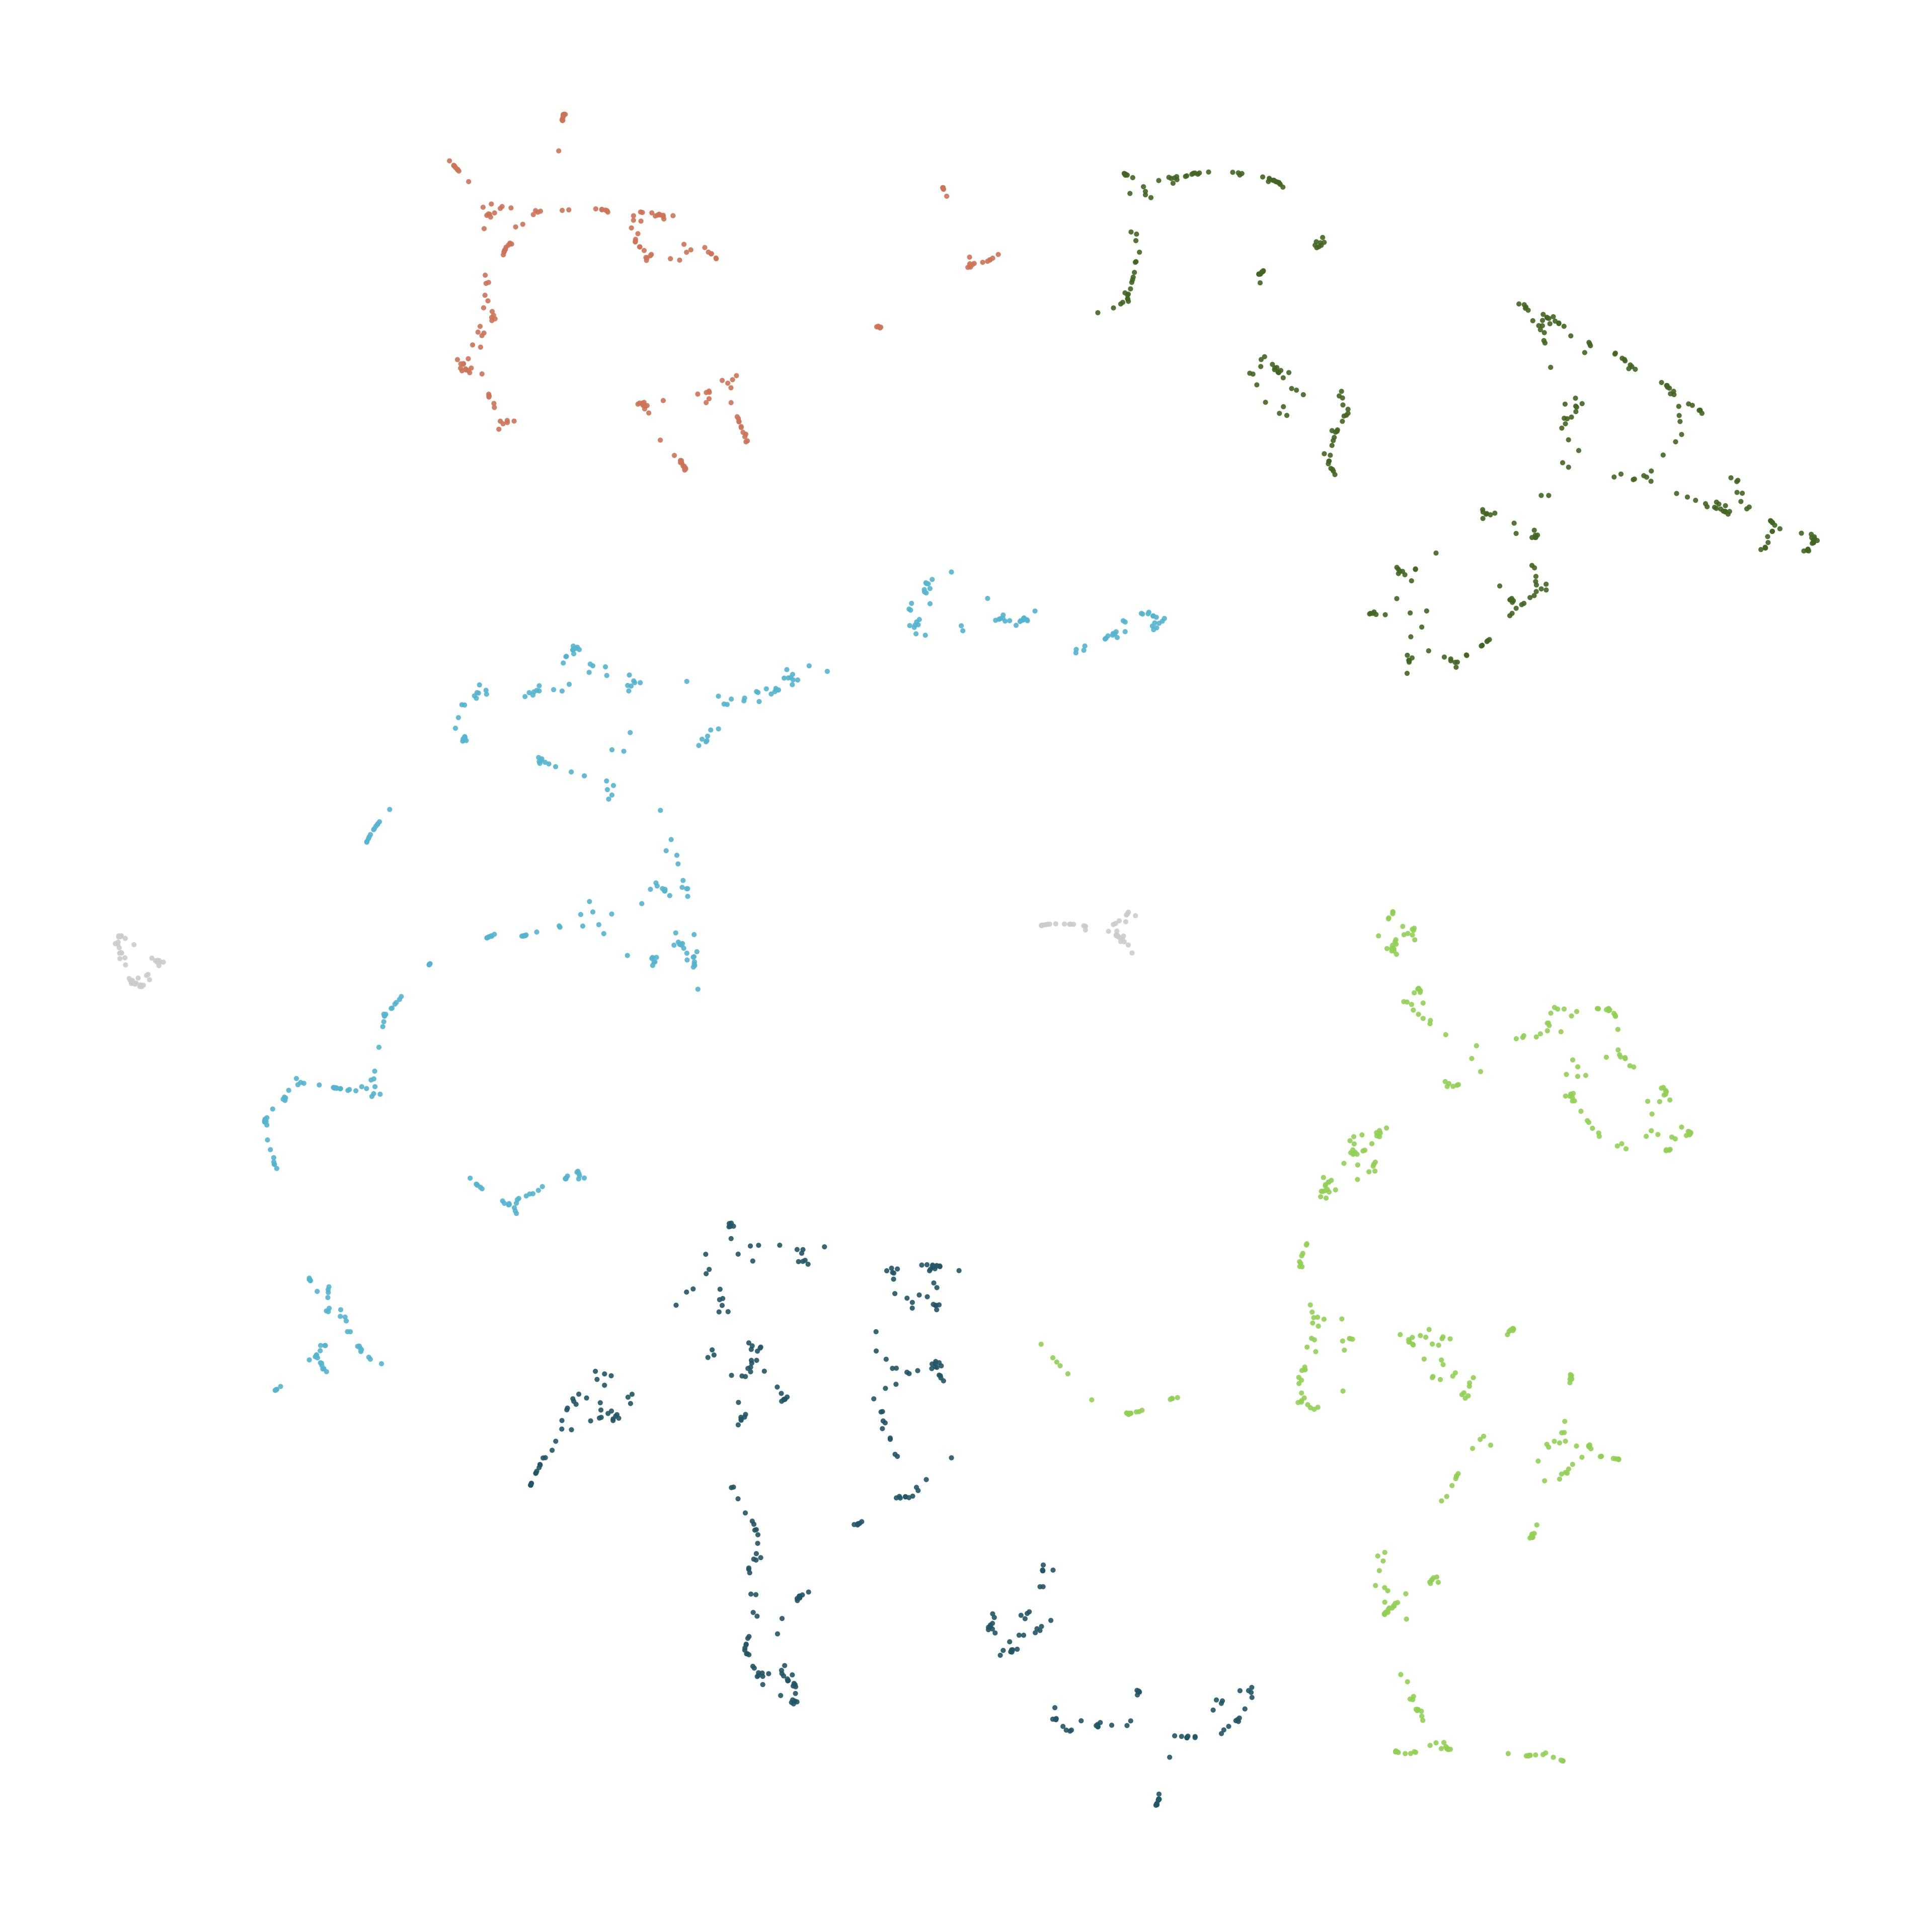
\includegraphics[width=\linewidth]{clusters/Dubai.jpg}
\end{minipage}\hfill
\begin{minipage}[t]{0.49\textwidth}
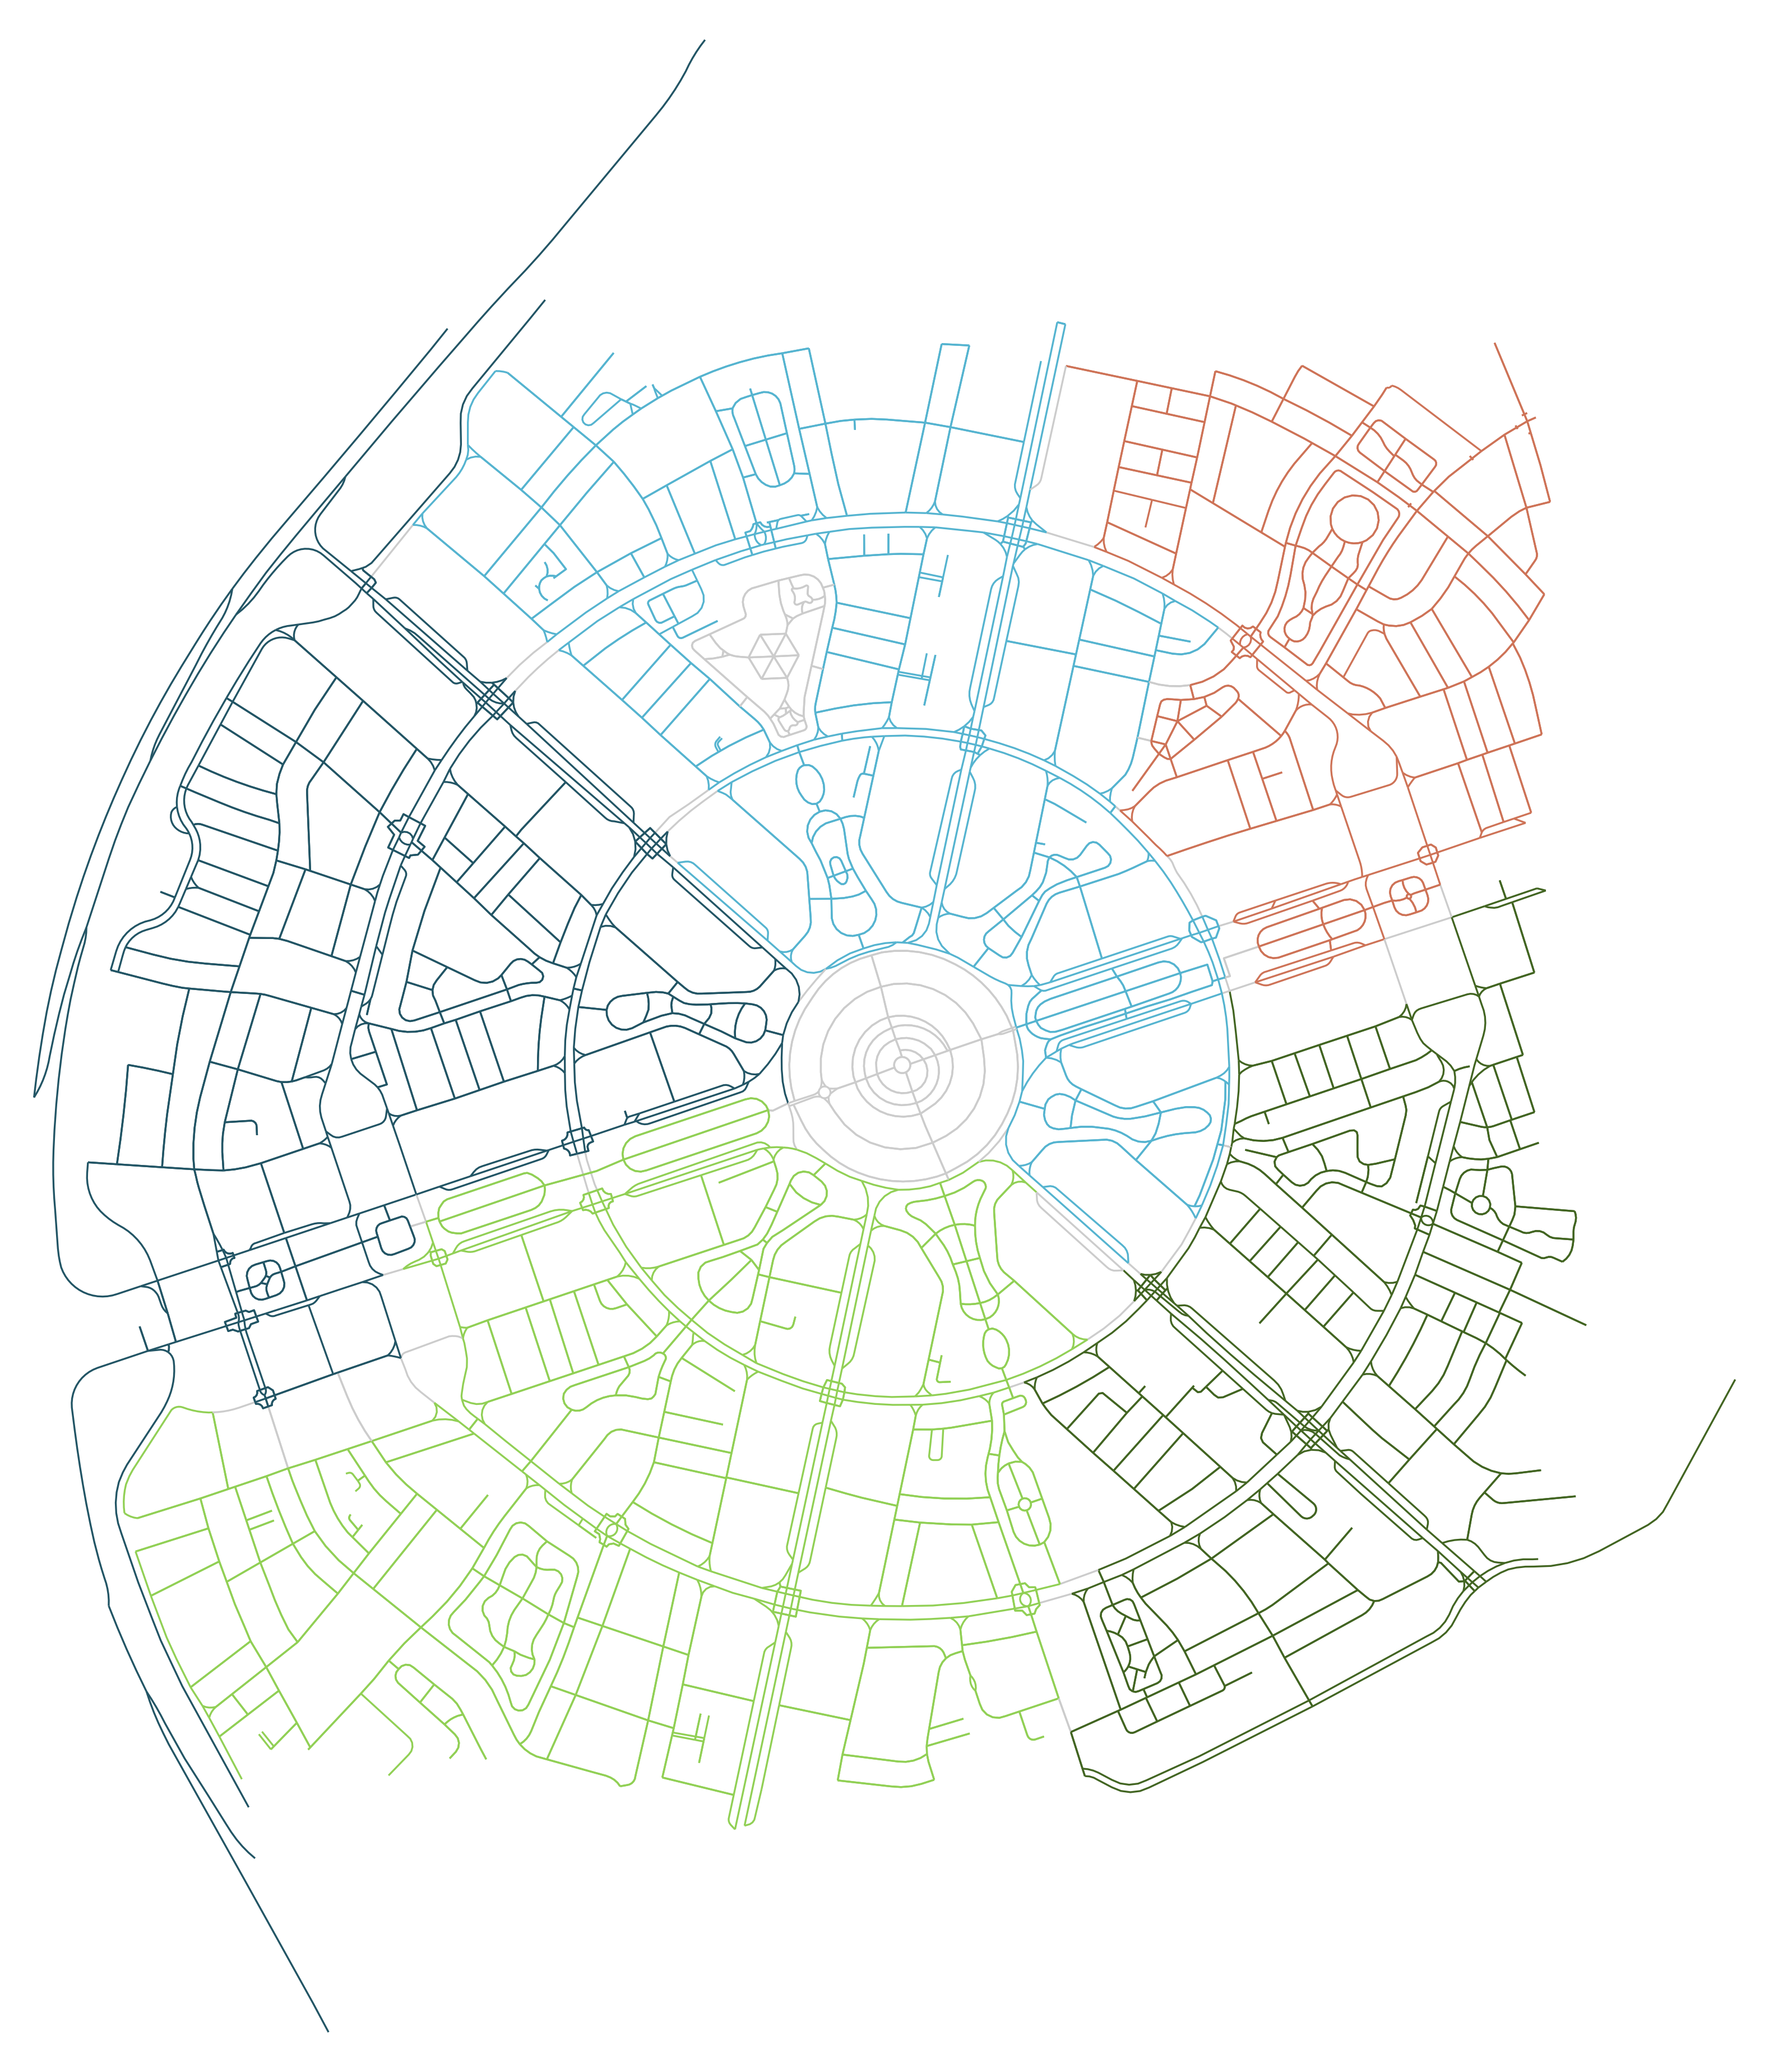
\includegraphics[width=\linewidth]{maps/Dubai.png}
\end{minipage}
\caption{Dubai. The embedding preserves the hexagonal “slices” of the city’s planned geometry, echoing the structural order visible in the map.}
\label{fig:dubai}
\end{figure}

\vspace{-10pt}
\begin{figure}[H]
\hspace{-3mm}
\begin{minipage}[t]{0.49\textwidth}
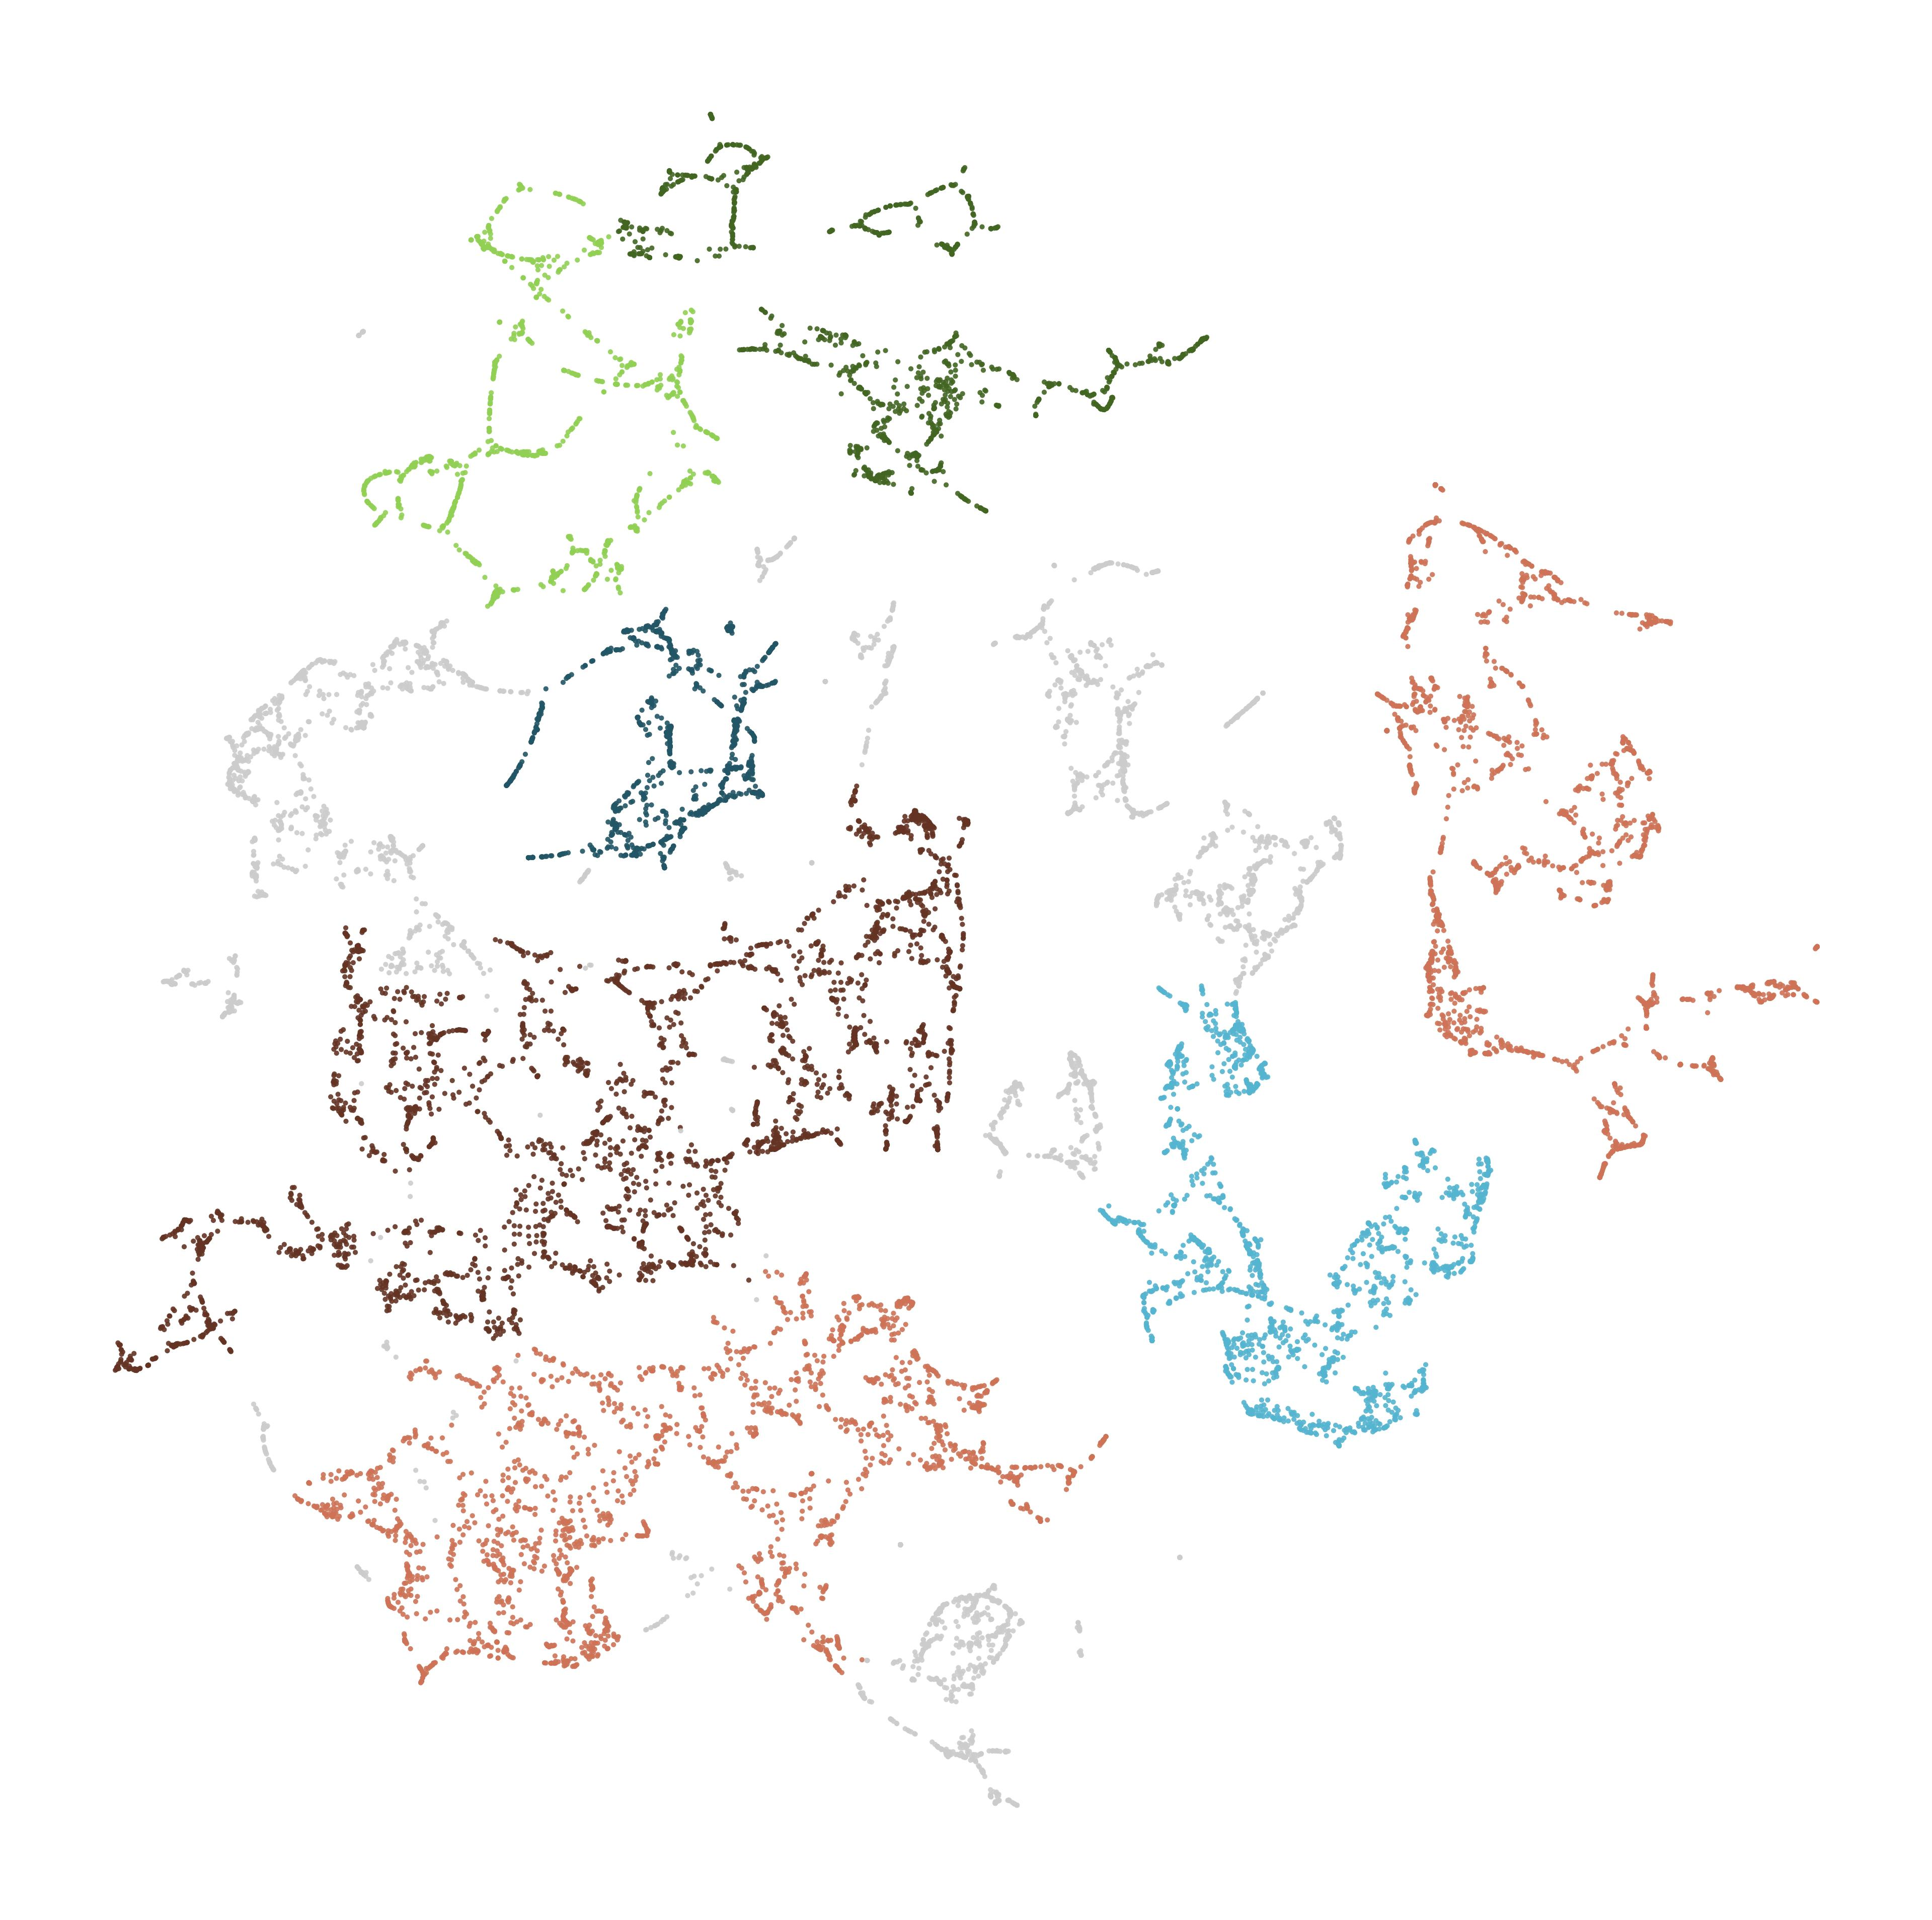
\includegraphics[width=\linewidth]{clusters/Canberra.jpg}
\end{minipage}\hfill
\begin{minipage}[t]{0.49\textwidth}
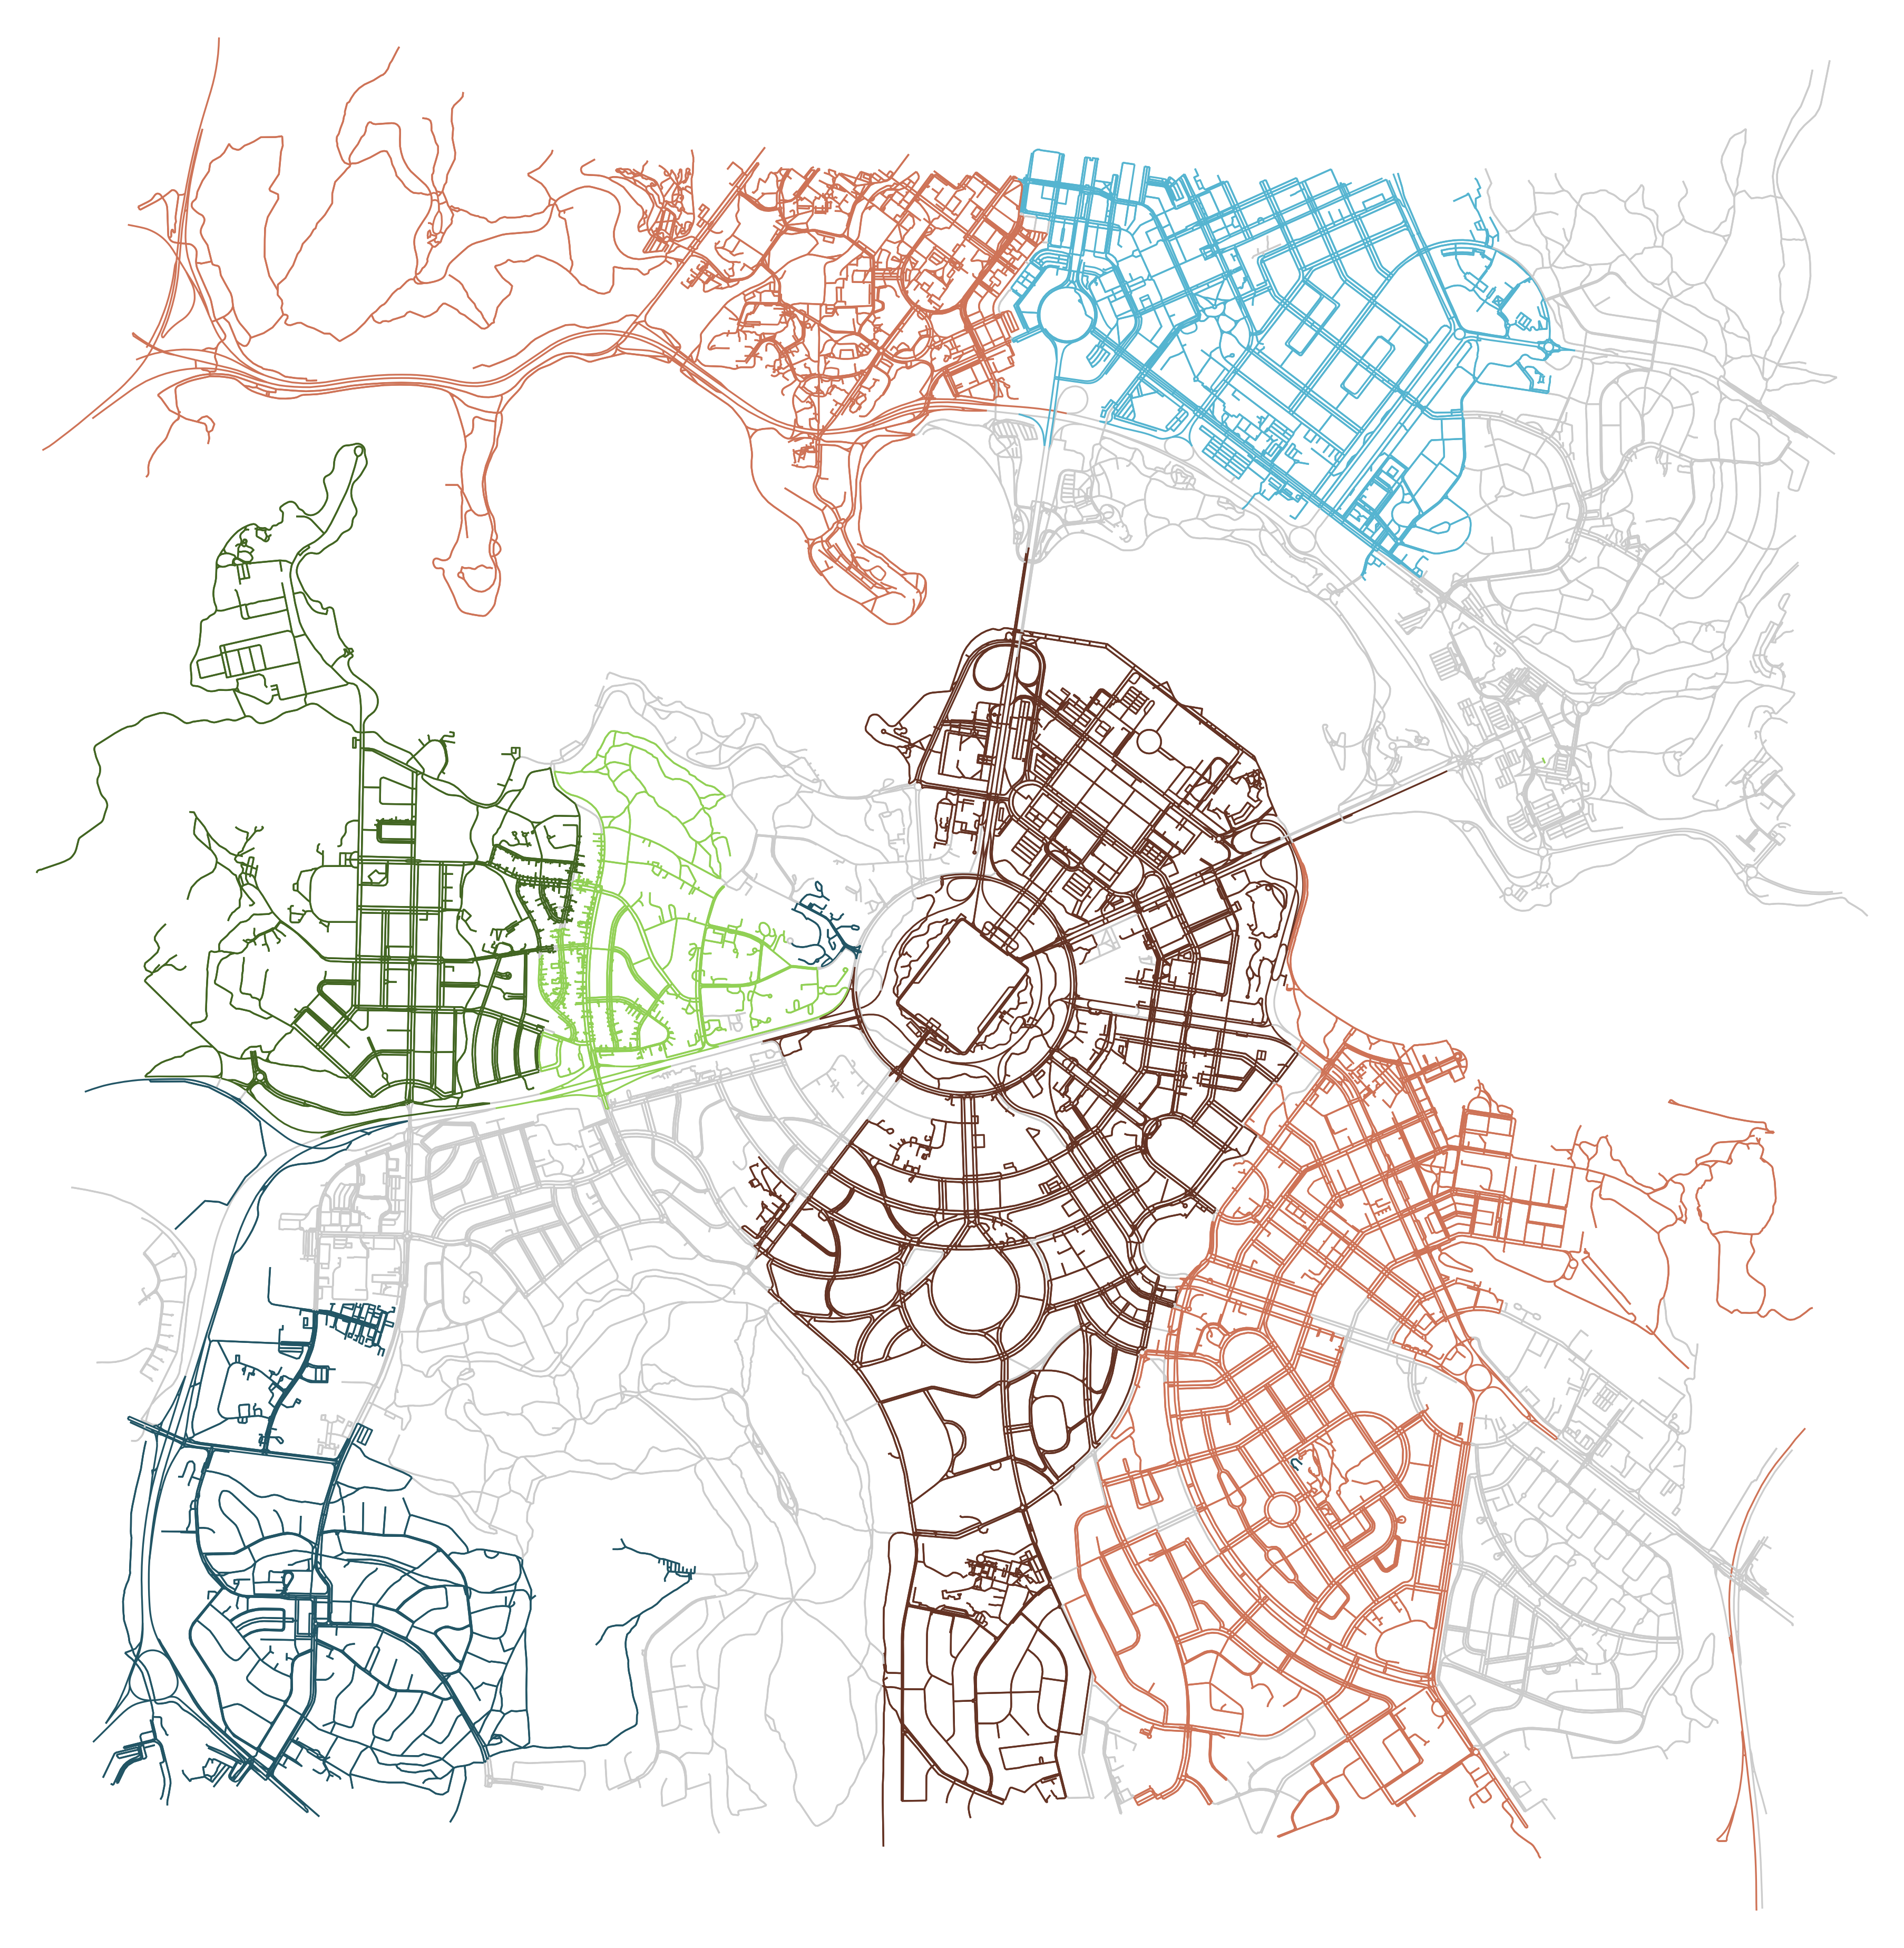
\includegraphics[width=\linewidth]{maps/Canberra.png}
\end{minipage}
\caption{Canberra. The embedding weakens the city’s formal geometry, yet neighborhoods remain coherent and spatially legible.}
\label{fig:canberra}
\end{figure}

The  {Relational} group (Table~\ref{table_relational_embeddings}) highlights the connectivity and polycentricity of urban fabrics. Cities such as Cairo and Berlin display neighborhoods as distinct but linked clusters, capturing the adjacencies that structure them. Berlin, in particular, reflects its history as an aggregation of multiple centers rather than a single unified plan. Los Angeles demonstrates another facet: while maps show residential areas interlaced with highways, embeddings separate them, highlighting weak ties that appear close cartographically.

An exemplary case is Amsterdam (Figure~\ref{fig:amsterdam}). The embedding faithfully reproduces the historical center and its ramified neighborhoods, while Amsterdam-Noord appears as a detached outlier, reflecting its infrastructural isolation. What the map shows as adjacency is reframed topologically as disconnection. This contrast underlines the city’s dual nature: a historically coherent core shaped by canals and expansion, and peripheral zones whose weak infrastructural ties become visible only through the embedding. 

\vspace{-8pt}
\begin{figure}[H]
\hspace{-3mm}
\begin{minipage}[t]{0.49\textwidth}
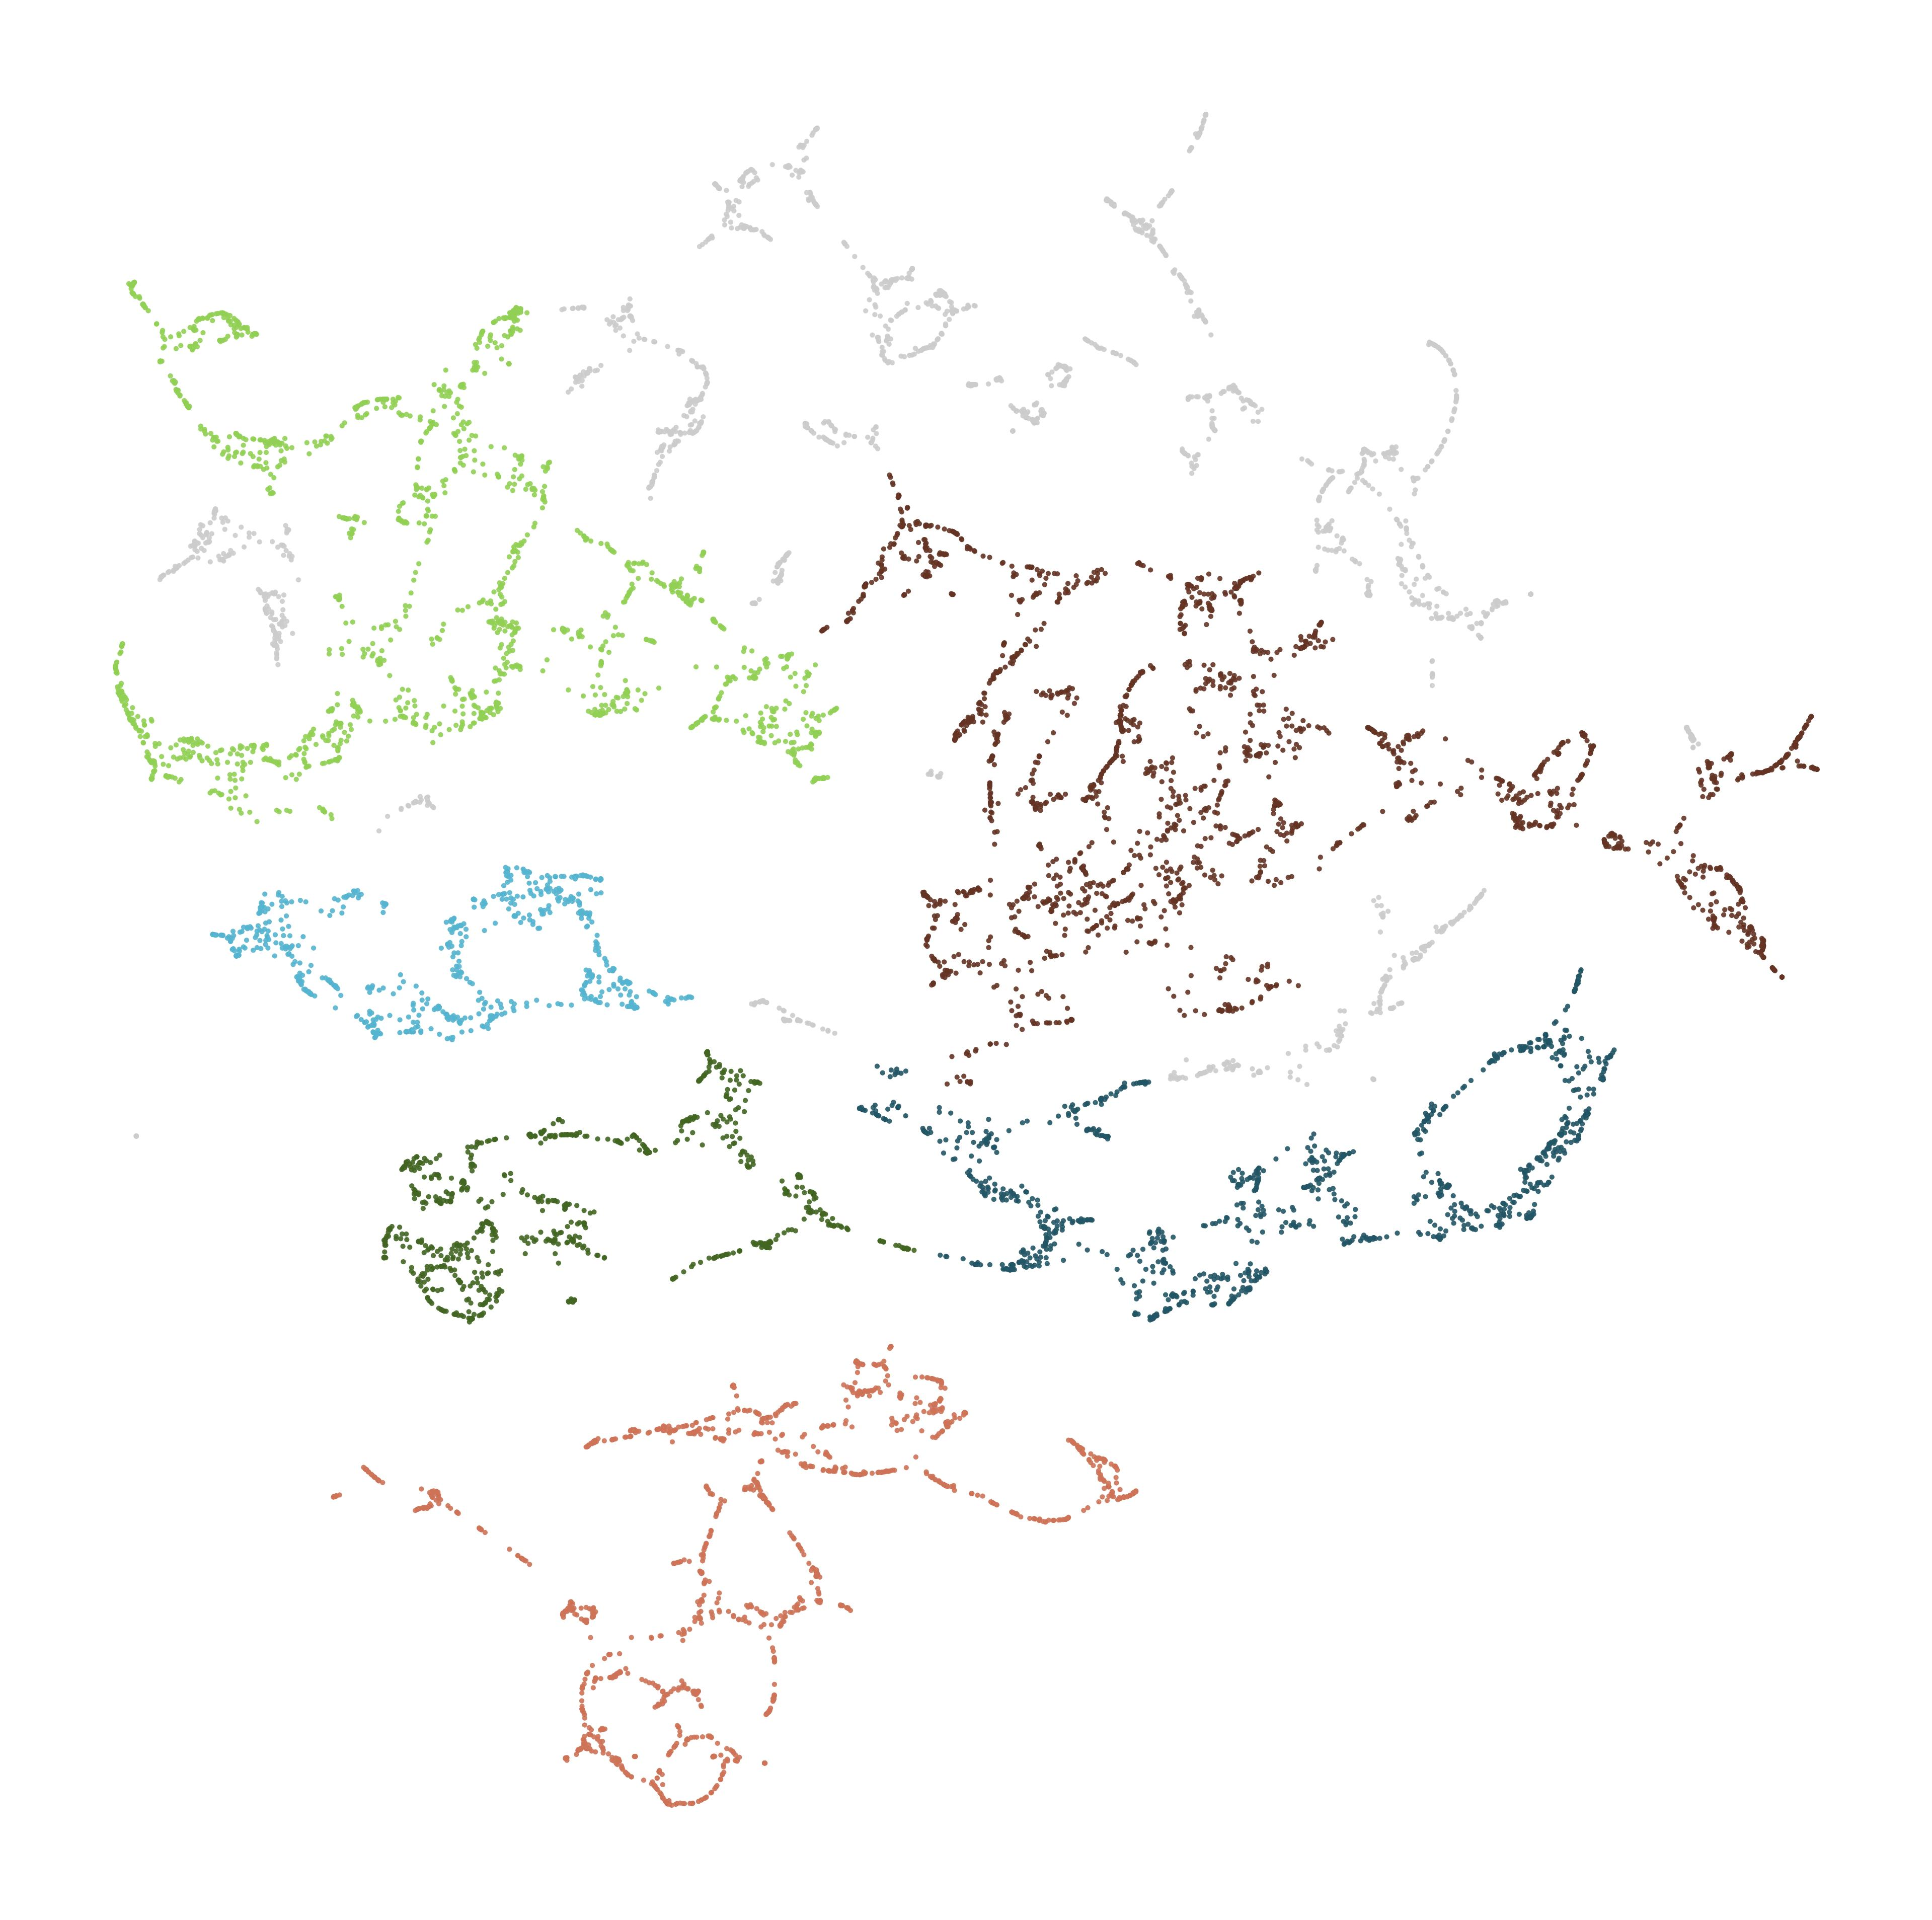
\includegraphics[width=\linewidth]{clusters/Amsterdam.jpg}
\end{minipage}\hfill
\begin{minipage}[t]{0.49\textwidth}
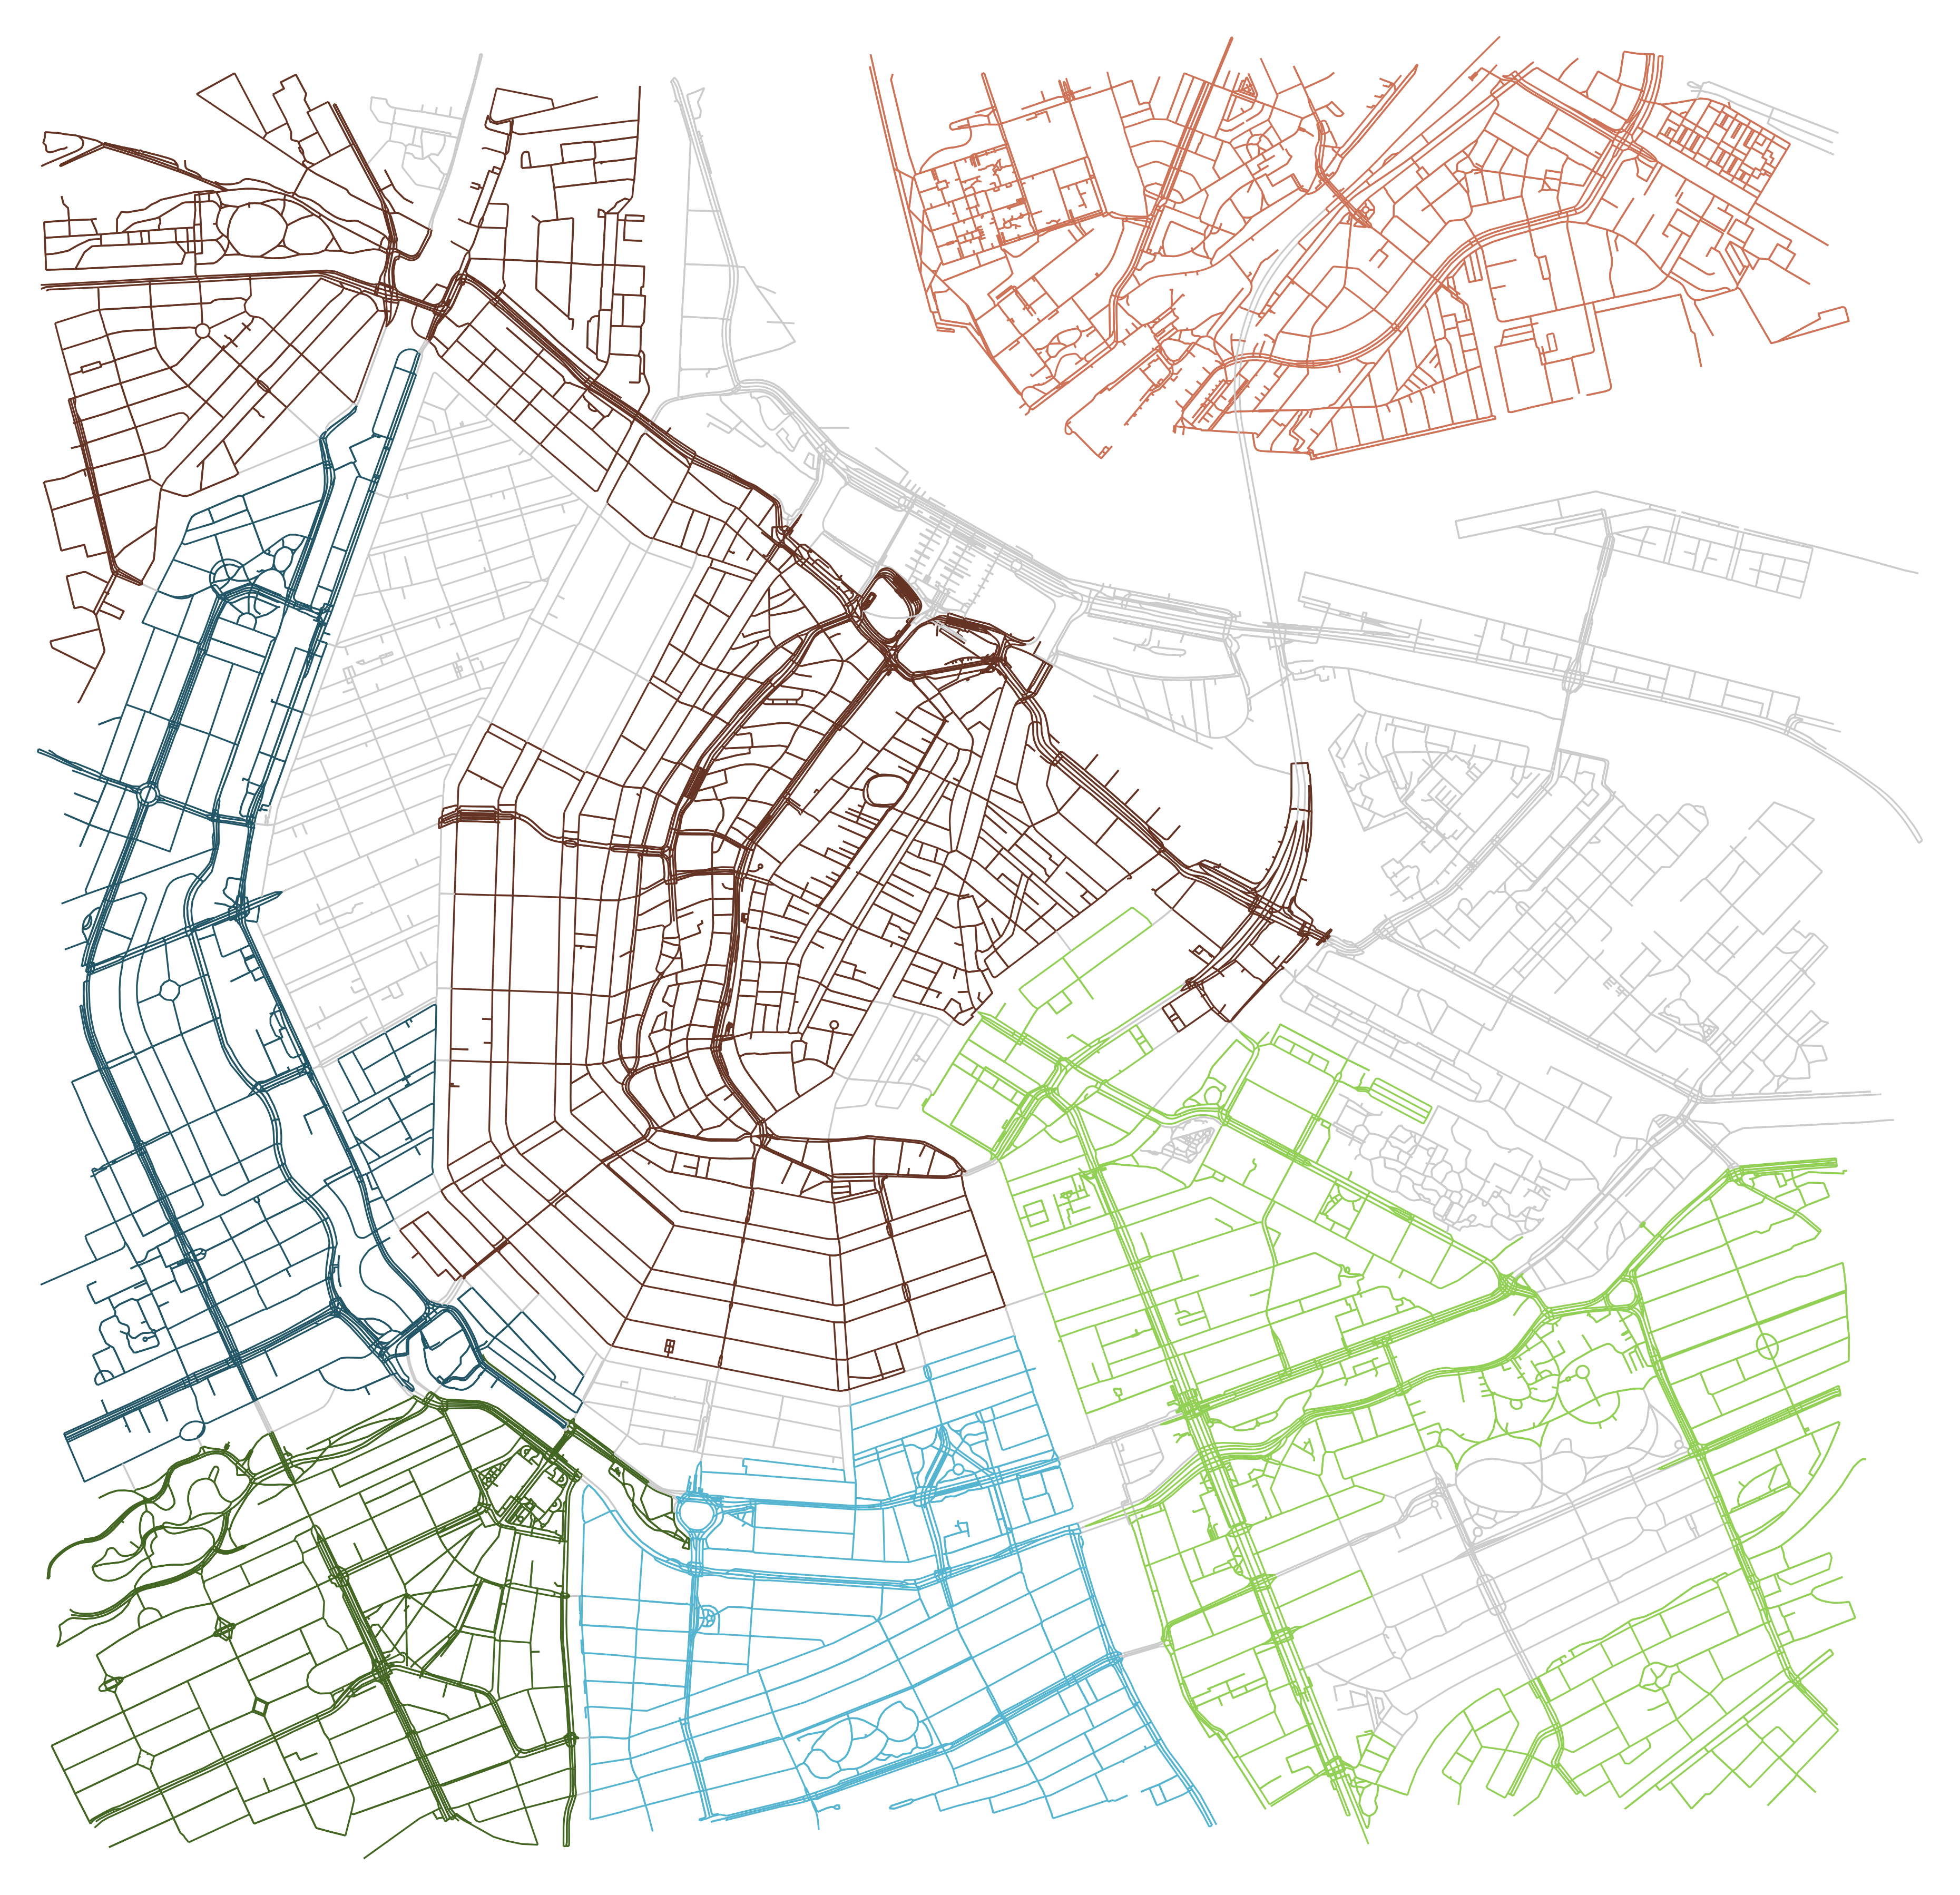
\includegraphics[width=\linewidth]{maps/Amsterdam.png}
\end{minipage}
\caption{Amsterdam. The embedding mirrors the ramified morphology of the historical center while detaching Amsterdam-Noord, visible as an isolated cluster.}
\label{fig:amsterdam}
\end{figure}

Taken together, these results show that the approach is most effective at small and medium scales. Compact cities and neighborhoods yield legible and often illuminating embeddings, while large metropolitan cases produce scattered and incoherent results. Scale thus emerges as a critical parameter: embeddings work best when urban fabrics are neither too microscopic nor too sprawling, but situated at an intermediate range where patterns of connectivity remain visible.

The embeddings also resonate with theoretical perspectives. They collapse junctions into focal points, producing computational analogues of \textit{{loci}}---intersections of movement and connectivity that shape urban experience. At the same time, they evoke the city as an assemblage: clusters that appear close in the embedding often correspond to highly connected realities, while distant clusters flag weak ties. Connectivity thus emerges at multiple levels---within nodes, between clusters, and across scales---providing an interpretative bridge between situated forms and broader relational associations.

Ultimately, the value of this method lies in its ability to extend cartography with topology. It shows how areas adjacent in physical space may be disconnected in terms of connectivity, or how infrastructural detachment becomes visible as separation in the embedding. Rather than replacing maps, it offers a complementary instrument: a photographic gun, in Yaneva and Latour’s sense, that allows designers to anticipate how cities move and change. \textit{{Network literacy}} thus gives urban designers an expanded vision, opening new ways of reasoning about the evolving fabric of the city.

%%%%%%%%%%%%%%%%%%%%%%%%%%%%%%%%%%%%%%%%%%%%%%%%%%%%%%%%%%%%%%%%%%%%%%%
%                       Embeddings - Maps                             %
%%%%%%%%%%%%%%%%%%%%%%%%%%%%%%%%%%%%%%%%%%%%%%%%%%%%%%%%%%%%%%%%%%%%%%%

\begin{table}[H]
\caption{Archetypal group of cities considered in this study: Rome (Italy), Vatican City (Vatican), Fez (Morocco), and Moscow (Russia). For each city, the table provides basic data, the UMAP+HDBSCAN embedding, and the colored map projection at the chosen scale, together with the taxonomy label from Lima’s classification.}
\label{table_archetypal_embeddings}

\begin{adjustwidth}{-\extralength}{0cm}
%\centering %% If there is a figure in wide page, please release command \centering
\begin{tabularx}{\fulllength}{>{\raggedright\arraybackslash}X m{6cm}<{\centering}m{6cm}<{\centering}}
\toprule
\textbf{City Info} & \multicolumn{1}{c}{\textbf{Embedding}} & \multicolumn{1}{c}{\textbf{Map}} \\[-0.5ex]
\midrule
\textbf{{Rome}} \newline Country: Italy \newline Lat/Lon: (41.8941, 12.4856) \newline Scale: 10 km \newline Group: Archetypal \newline Taxonomy Label: \newline Radial Implosion &
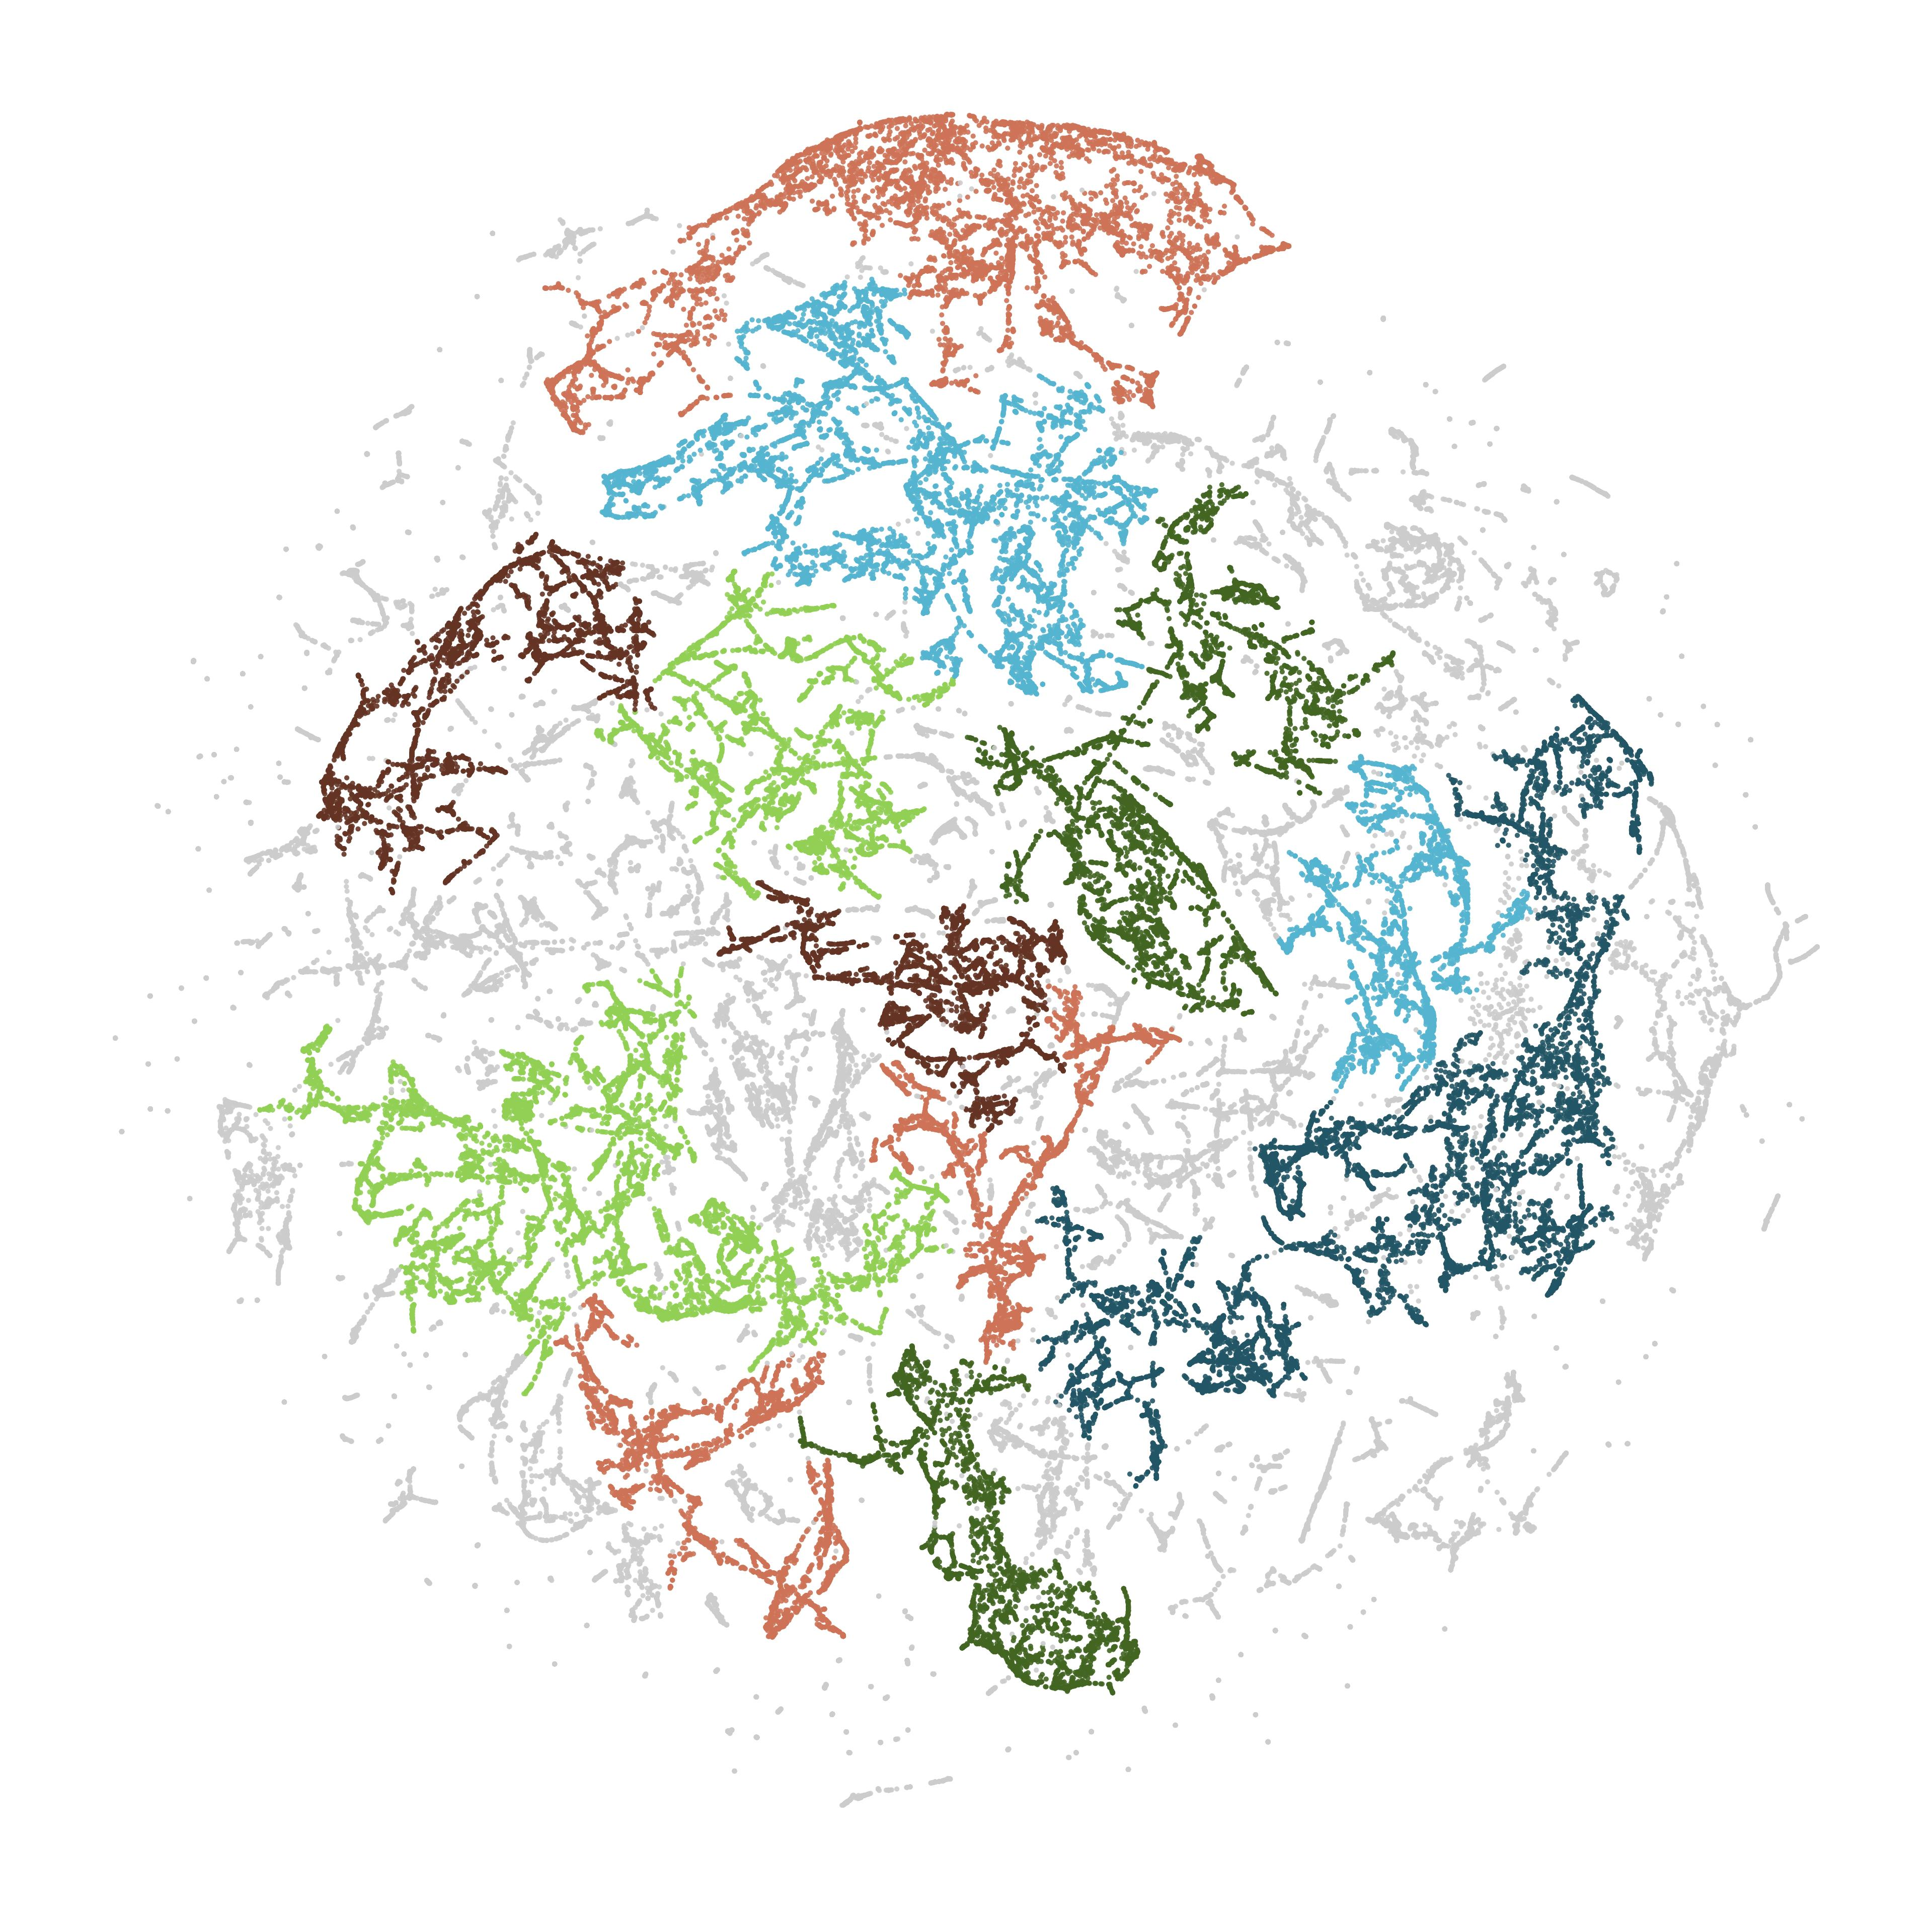
\includegraphics[width=0.85\linewidth]{clusters/Rome.jpg} &
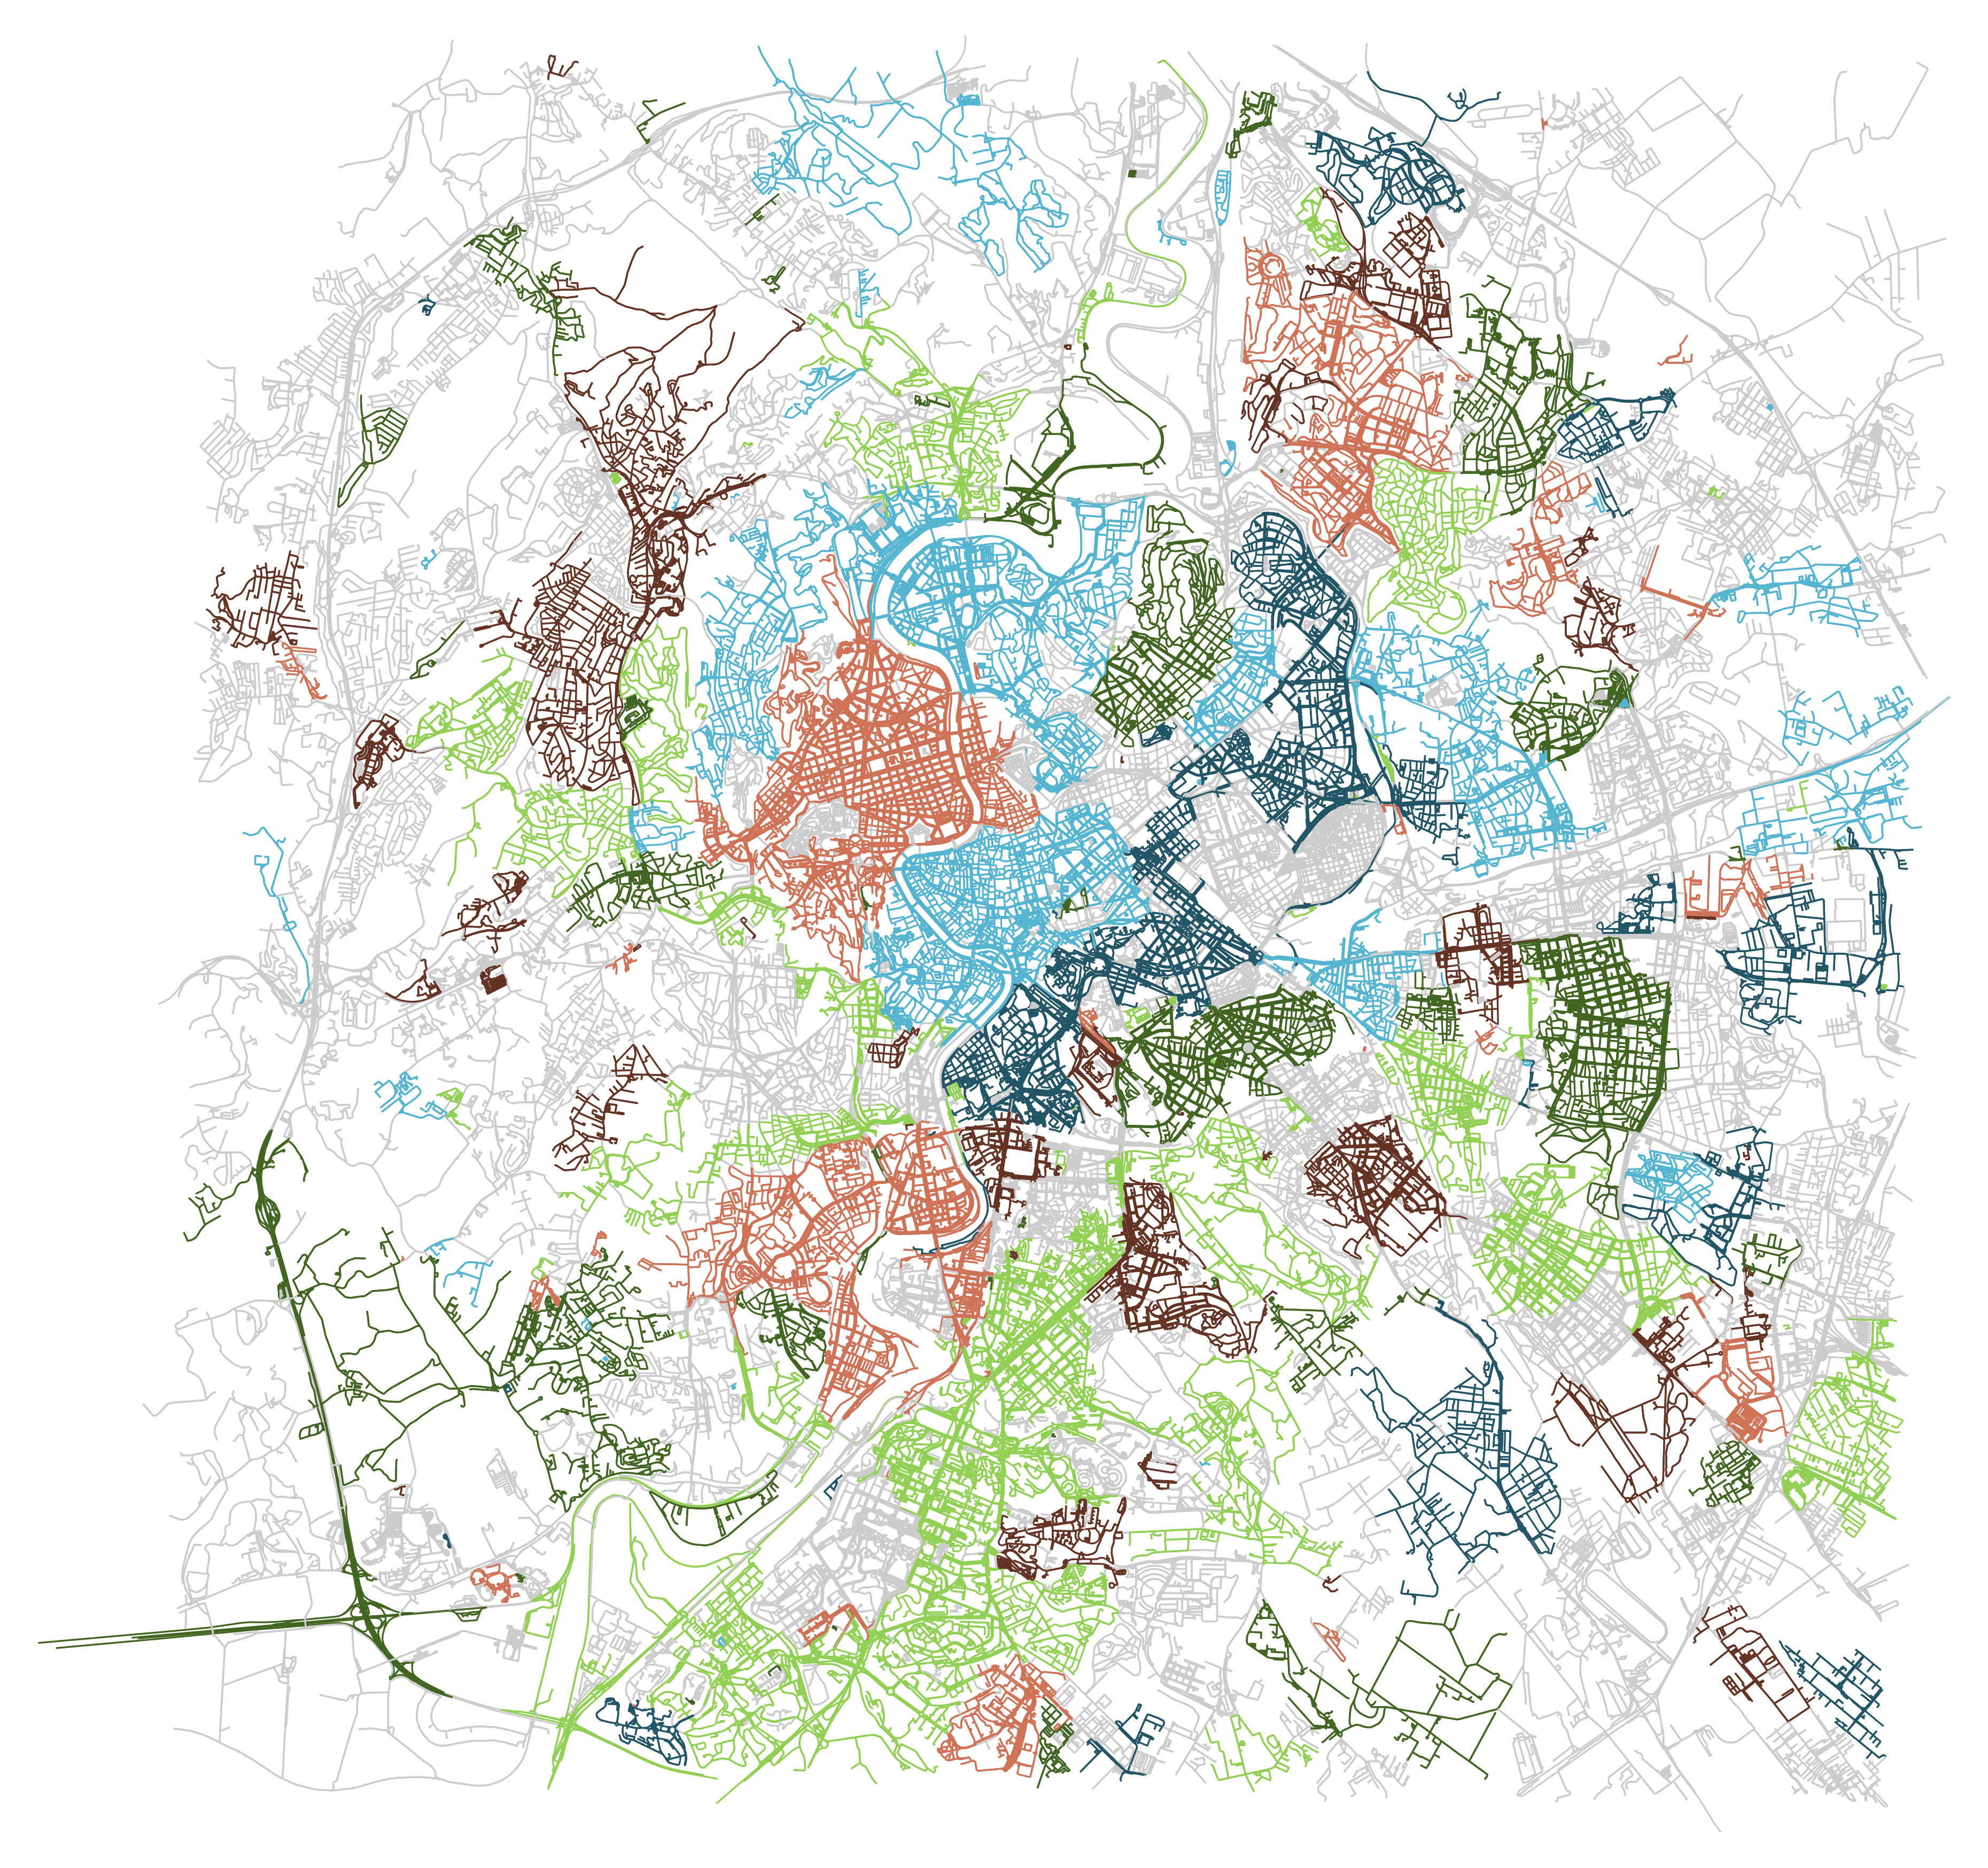
\includegraphics[width=0.85\linewidth]{maps/Rome.png} \\[-1.5ex]
\midrule
\textbf{{Vatican City}} \newline Country: Vatican \newline Lat/Lon: (41.9023, 12.4574) \newline Scale: 1 km \newline Group: Archetypal \newline Taxonomy Label: \newline Elliptical Implosion &
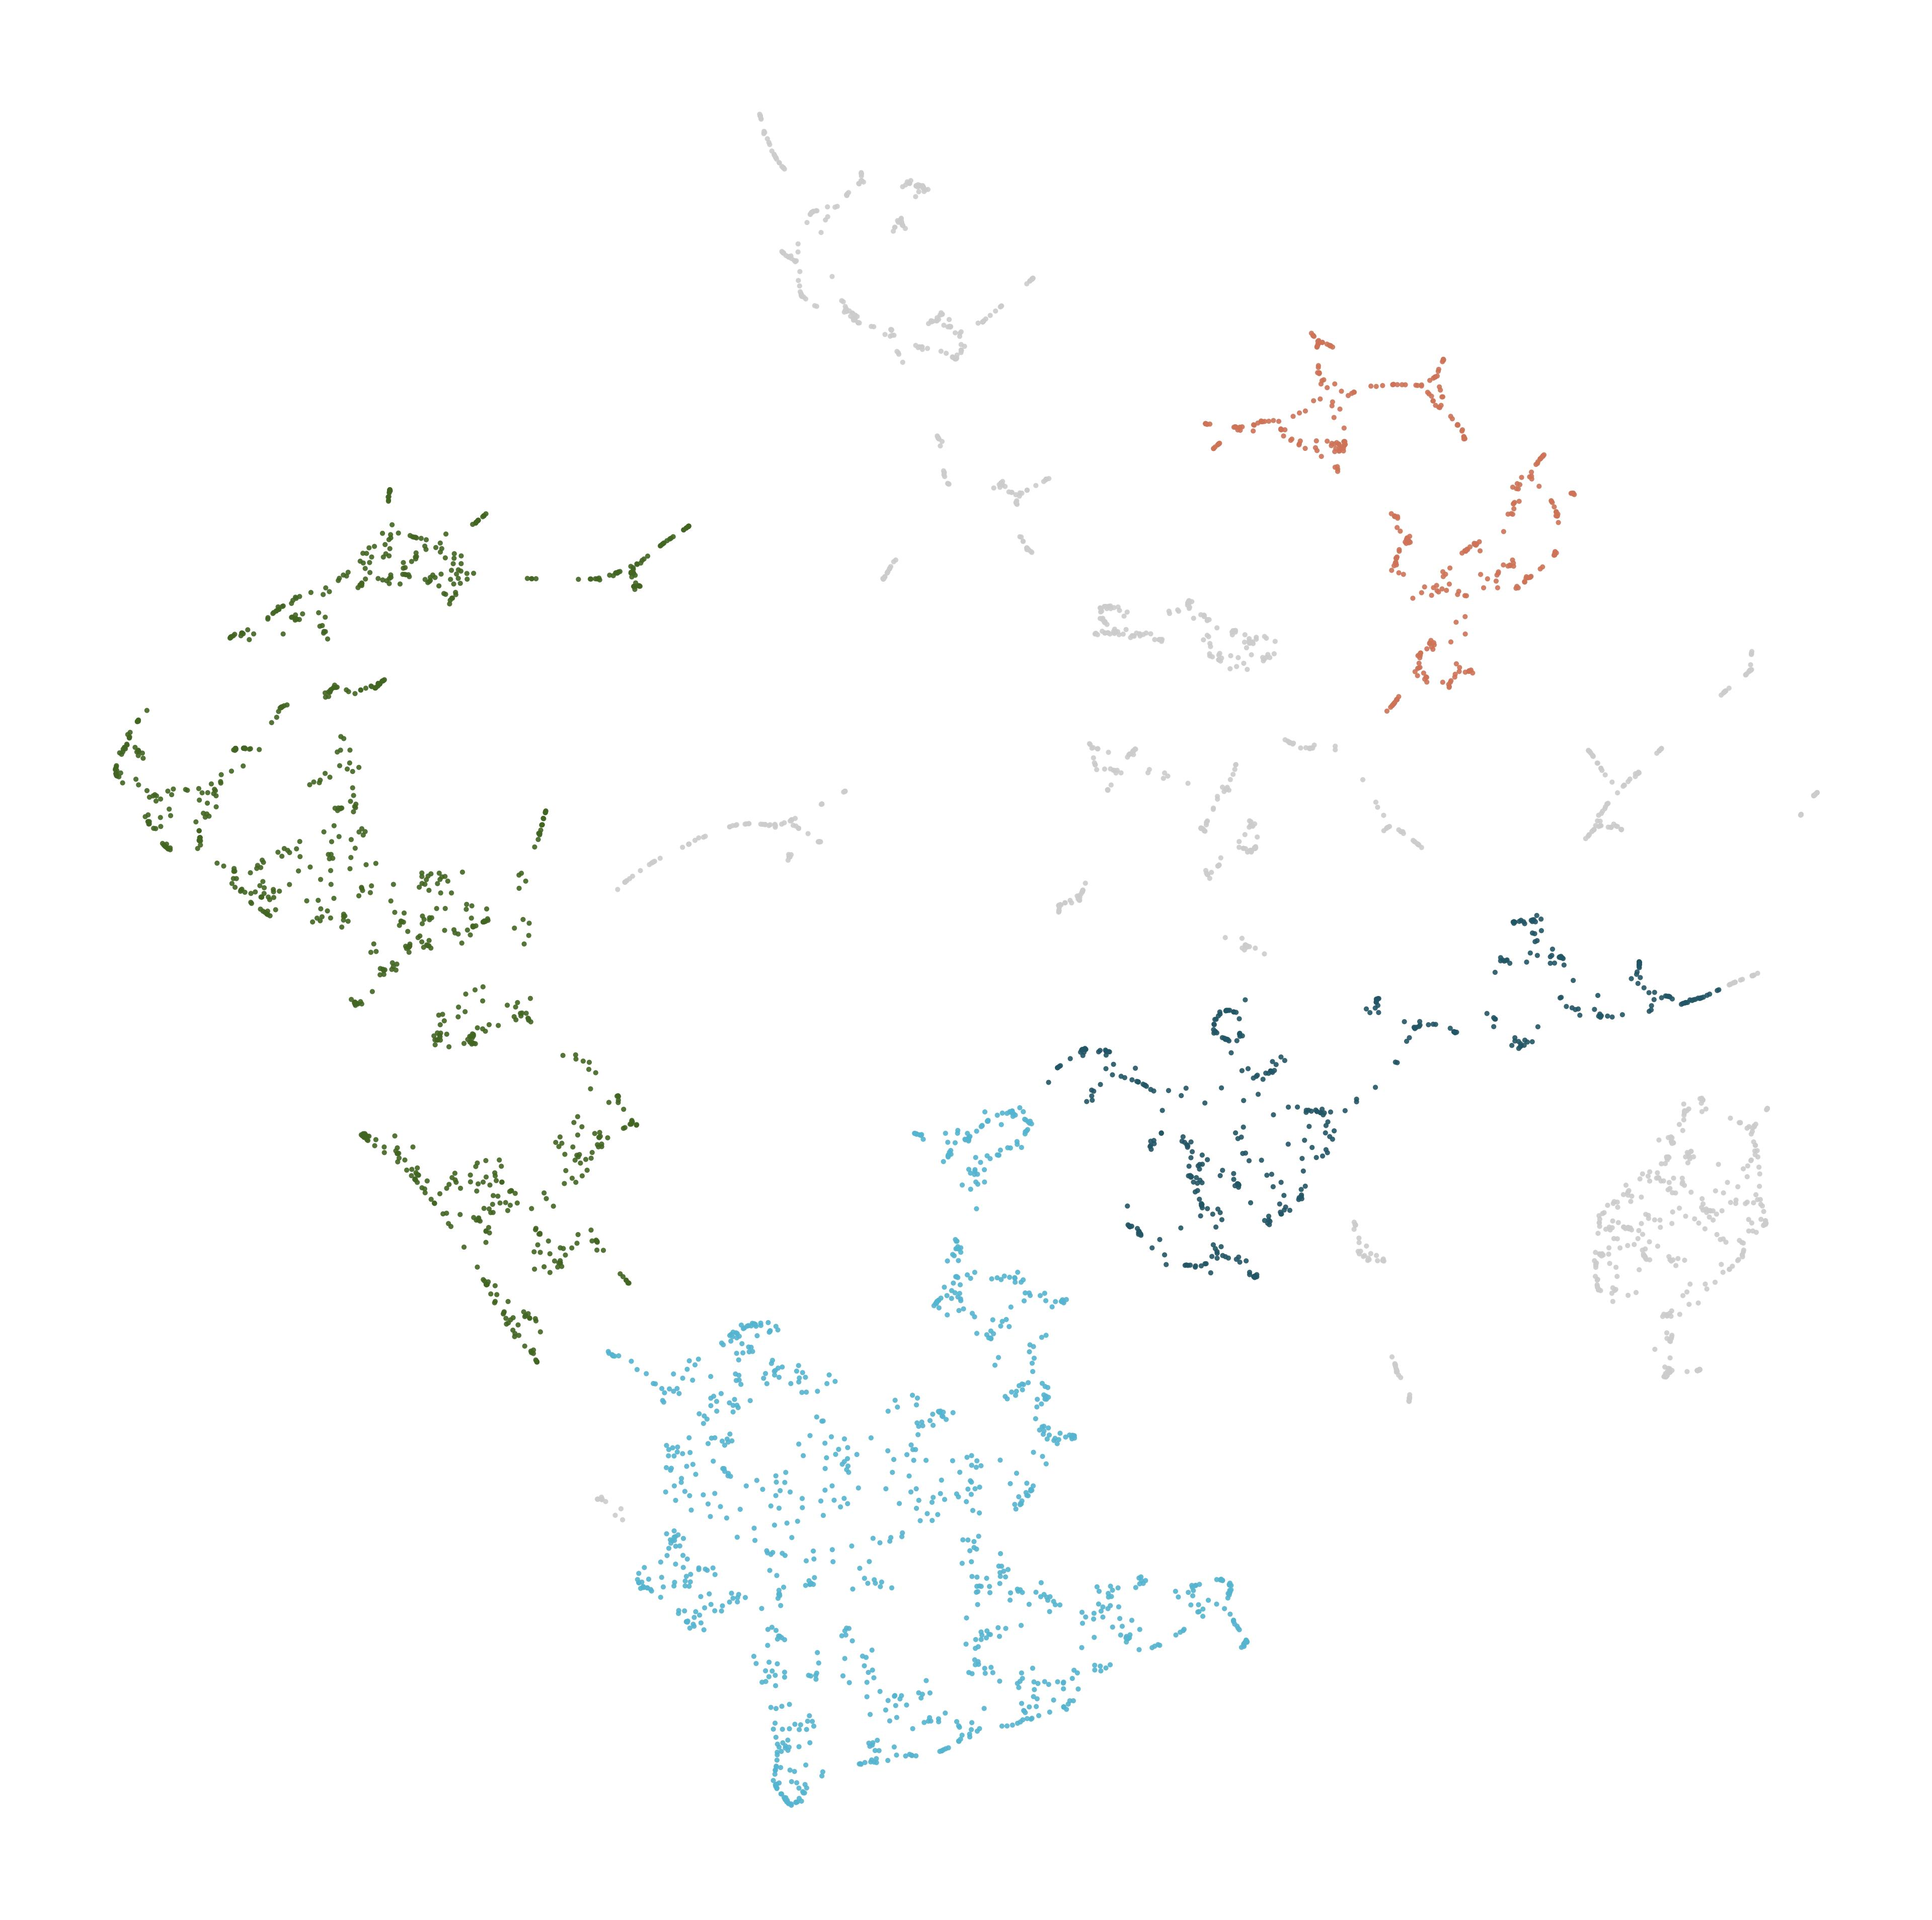
\includegraphics[width=0.85\linewidth]{clusters/Vatican_City.jpg} &
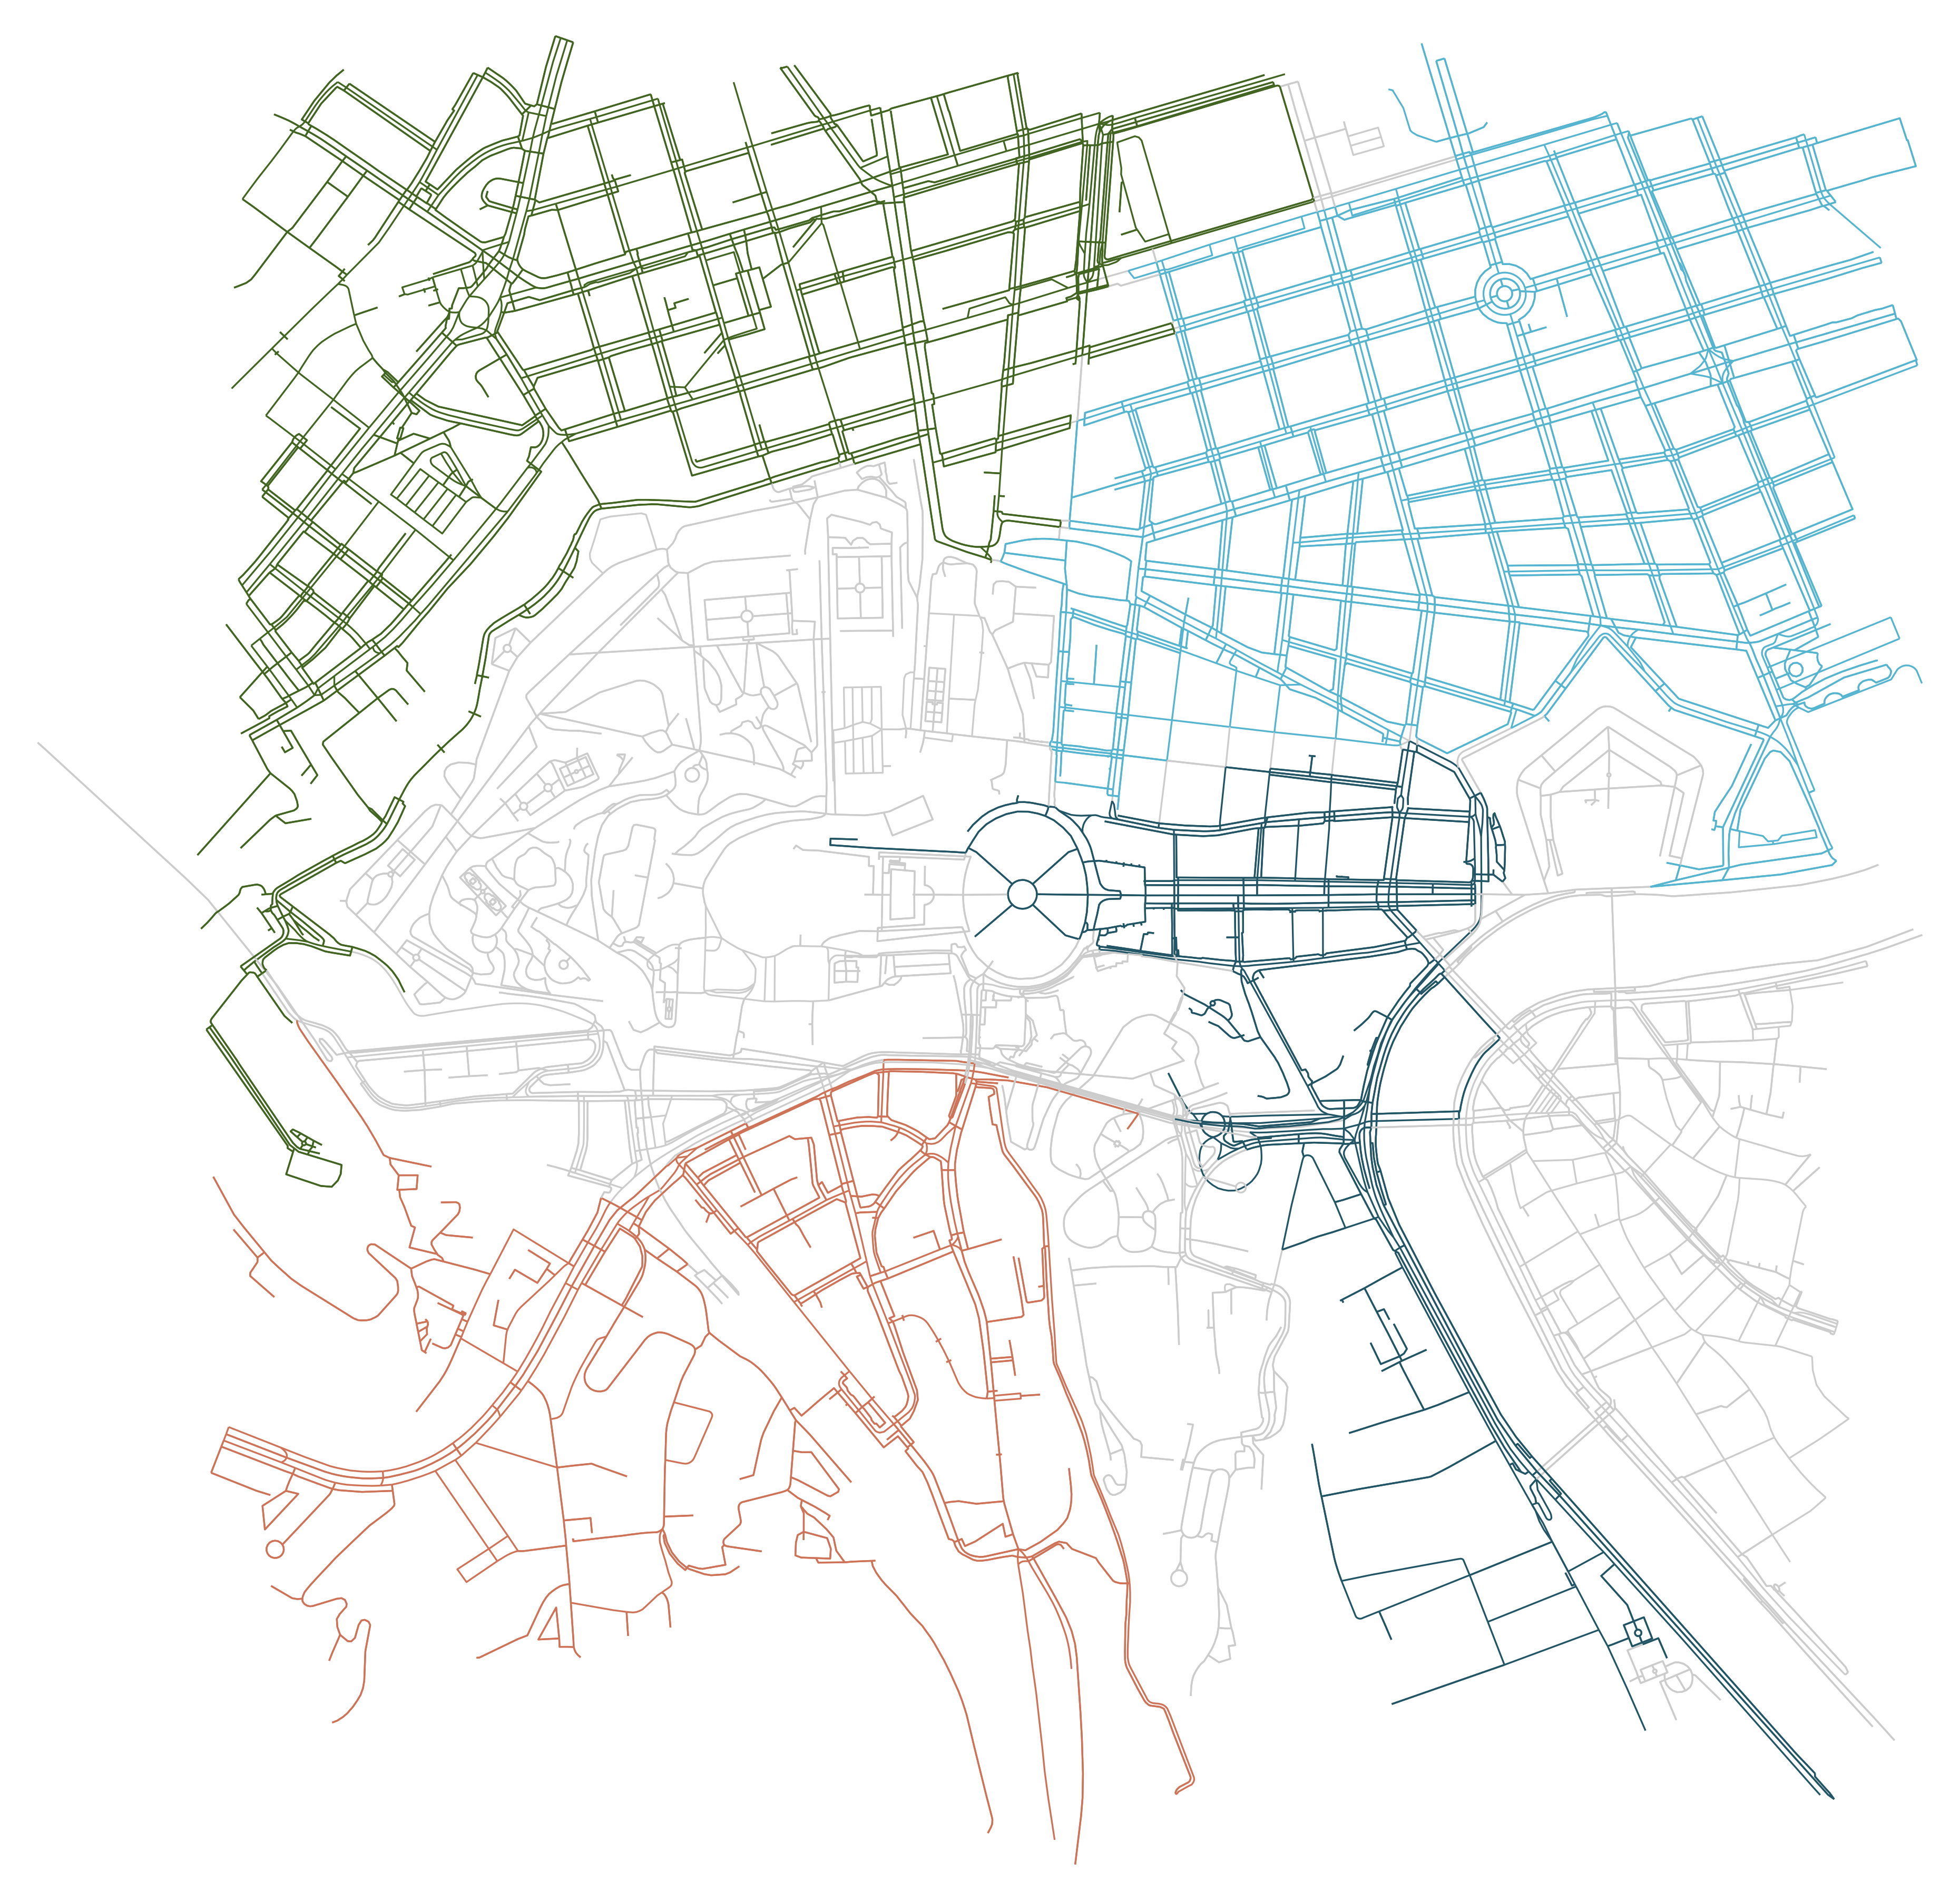
\includegraphics[width=0.85\linewidth]{maps/Vatican_City.png} \\[-0.5ex]
\midrule
\textbf{{Fez}} \newline Country: Morocco \newline Lat/Lon: (34.0650, $-$4.9730) \newline Scale: 1 km \newline Group: Archetypal \newline Taxonomy Label: \newline Organic Rhizome &
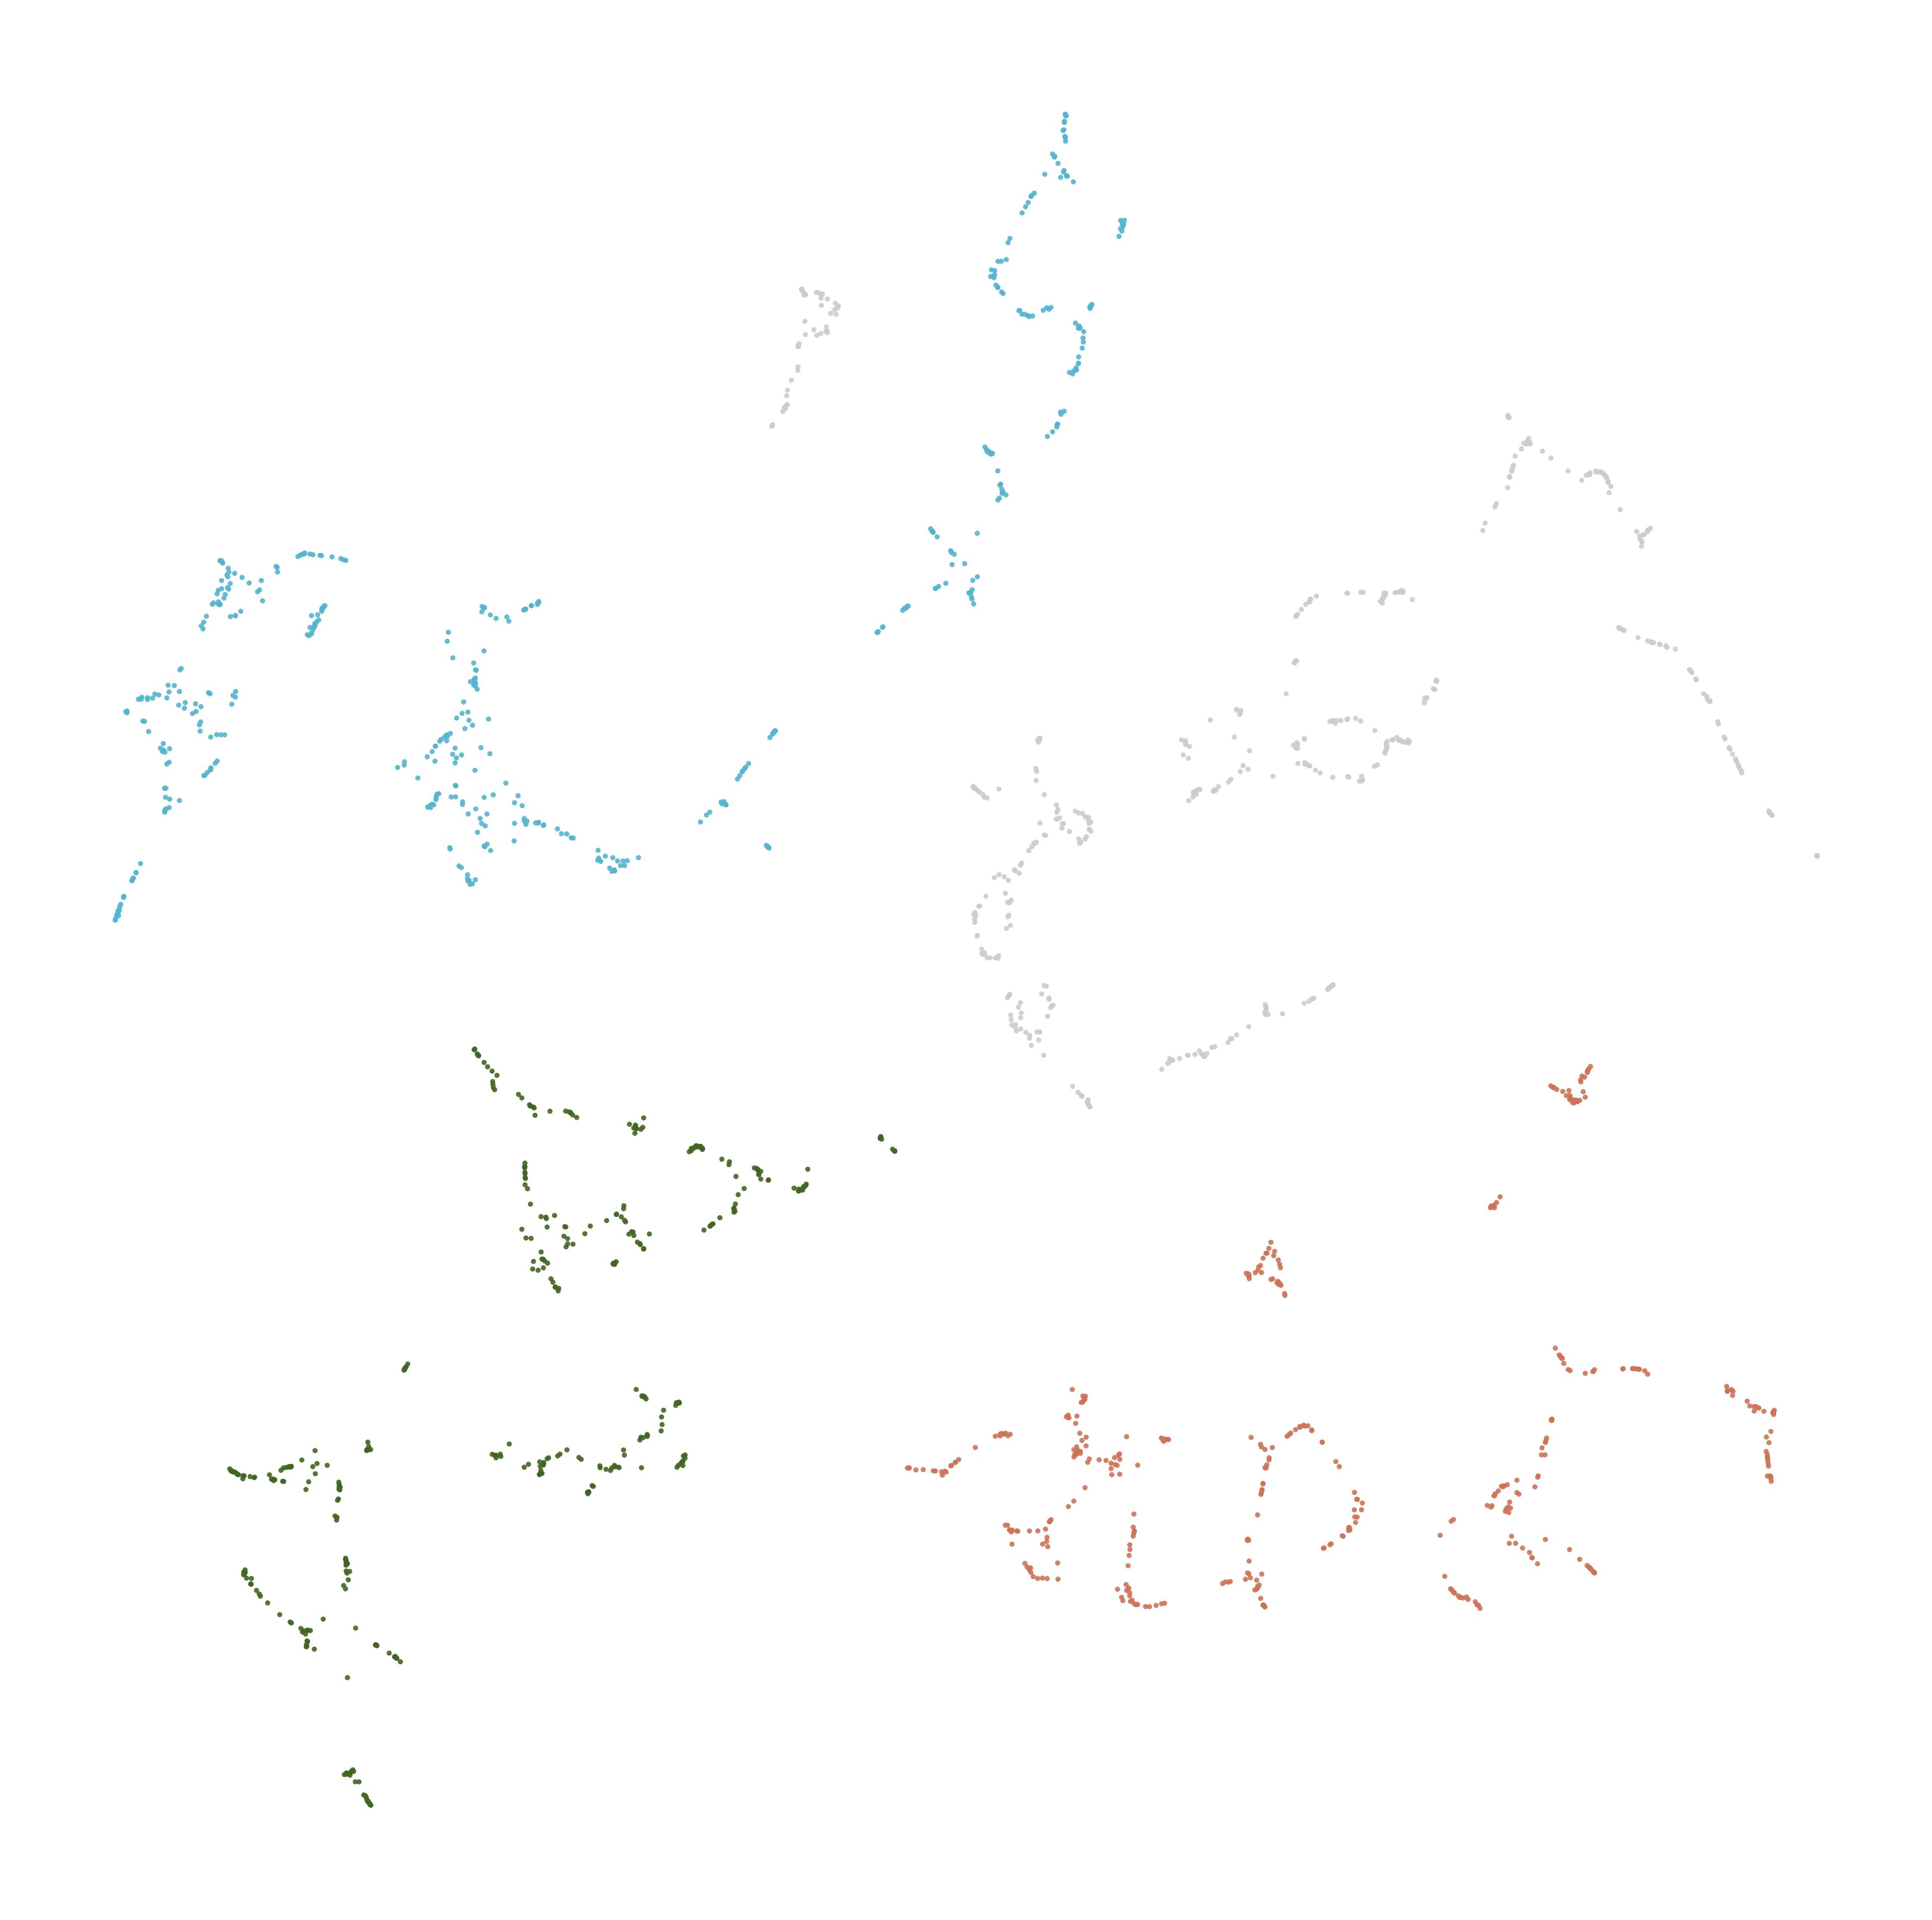
\includegraphics[width=0.85\linewidth]{clusters/Fez.jpg} &
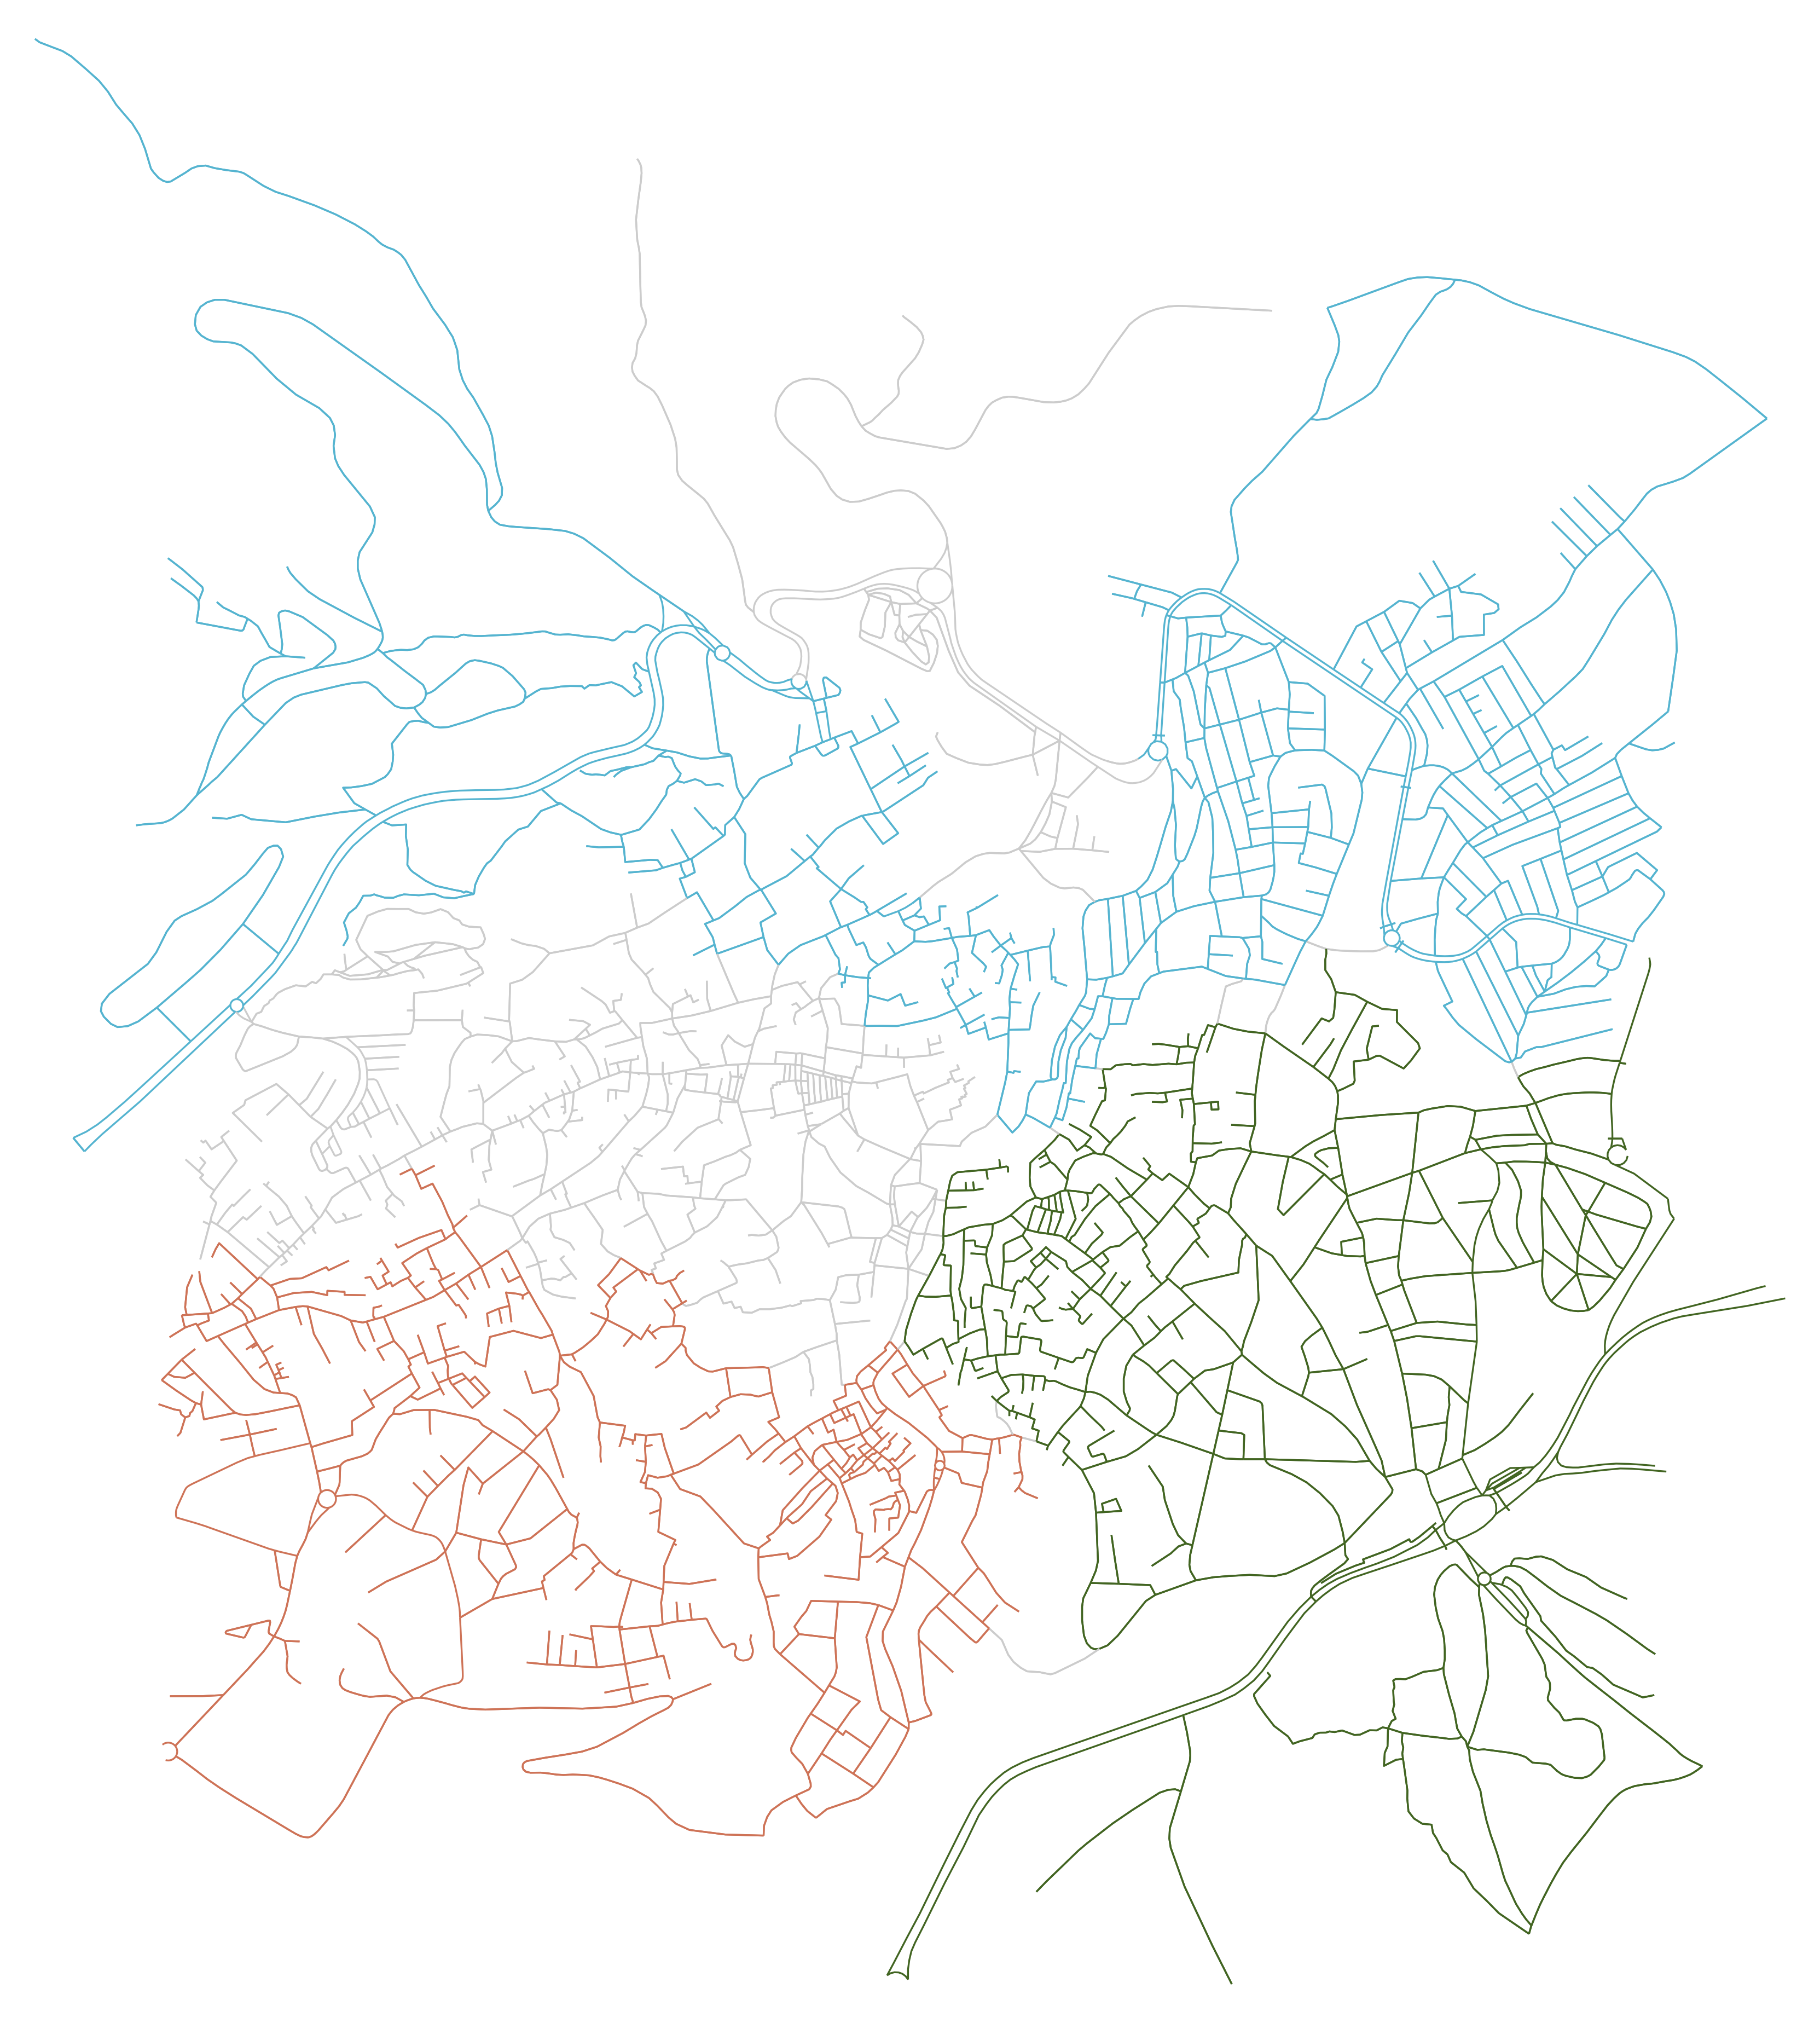
\includegraphics[width=0.85\linewidth]{maps/Fez.png} \\[-0.5ex]
\midrule
\textbf{{Moscow}} \newline Country: Russia \newline Lat/Lon: (55.7558, 37.6176) \newline Scale: 5 km \newline Group: Archetypal \newline Taxonomy Label: \newline Centralized Burst &
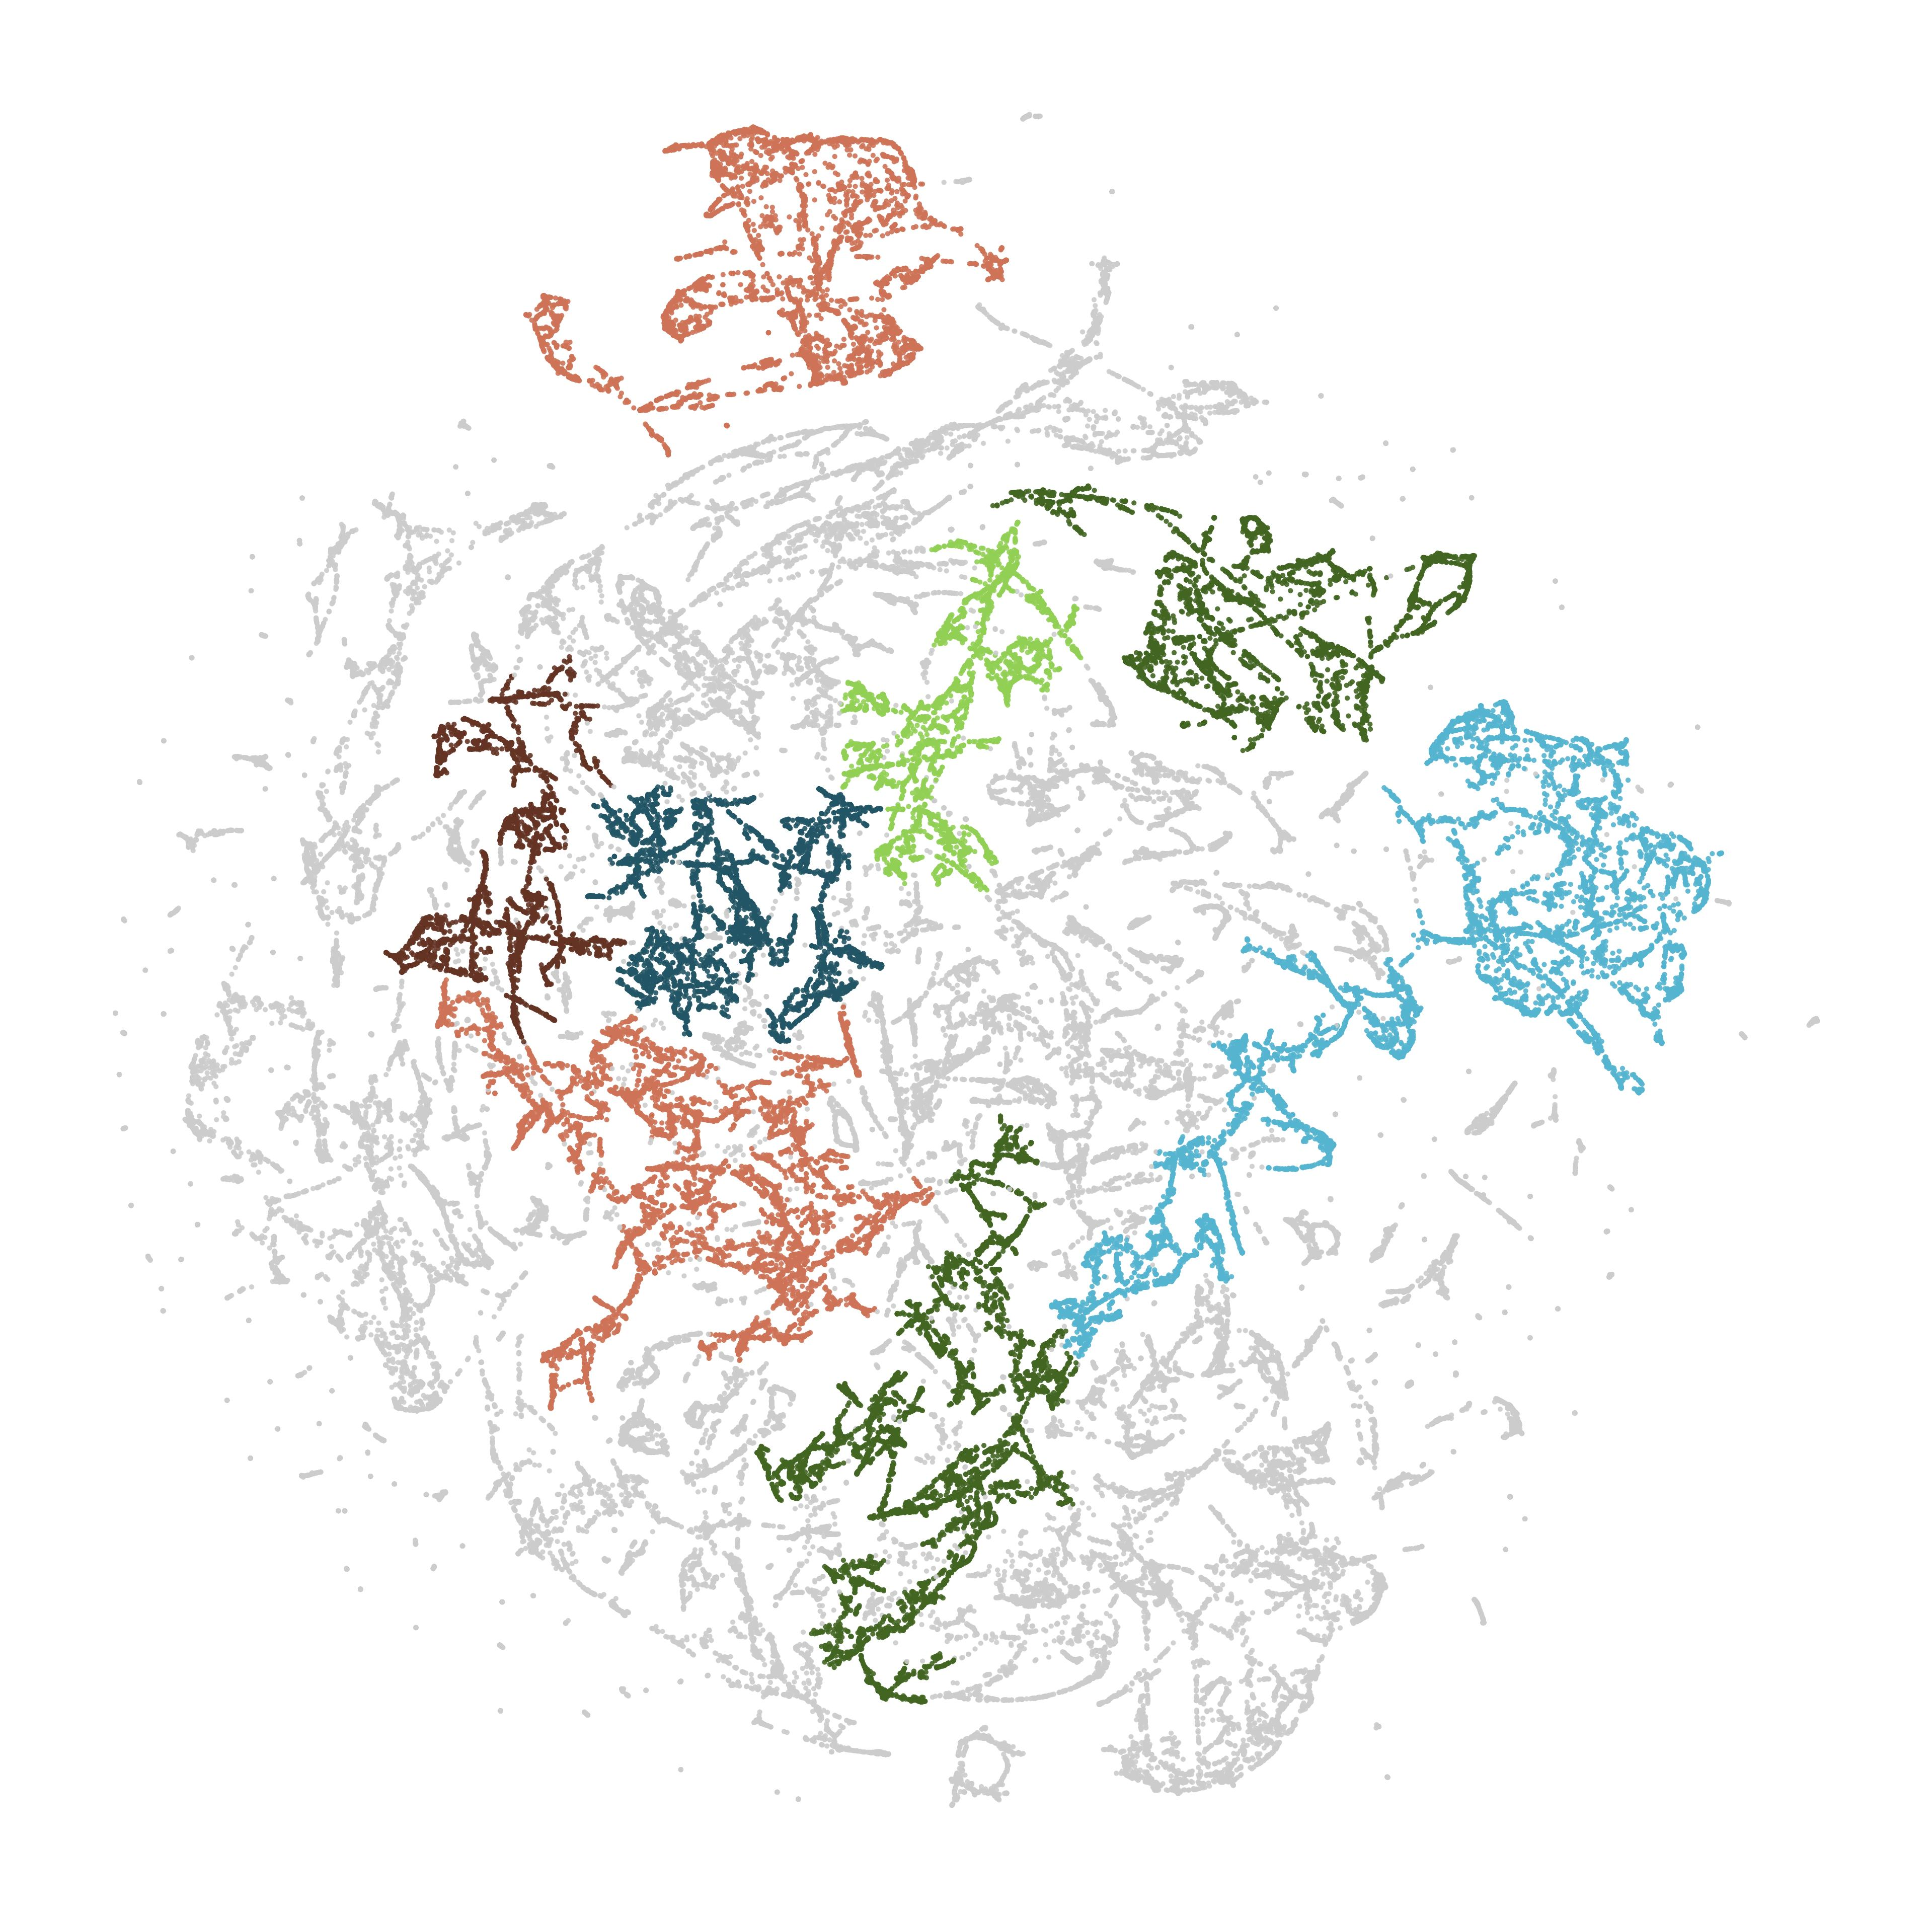
\includegraphics[width=0.85\linewidth]{clusters/Moscow.jpg} &
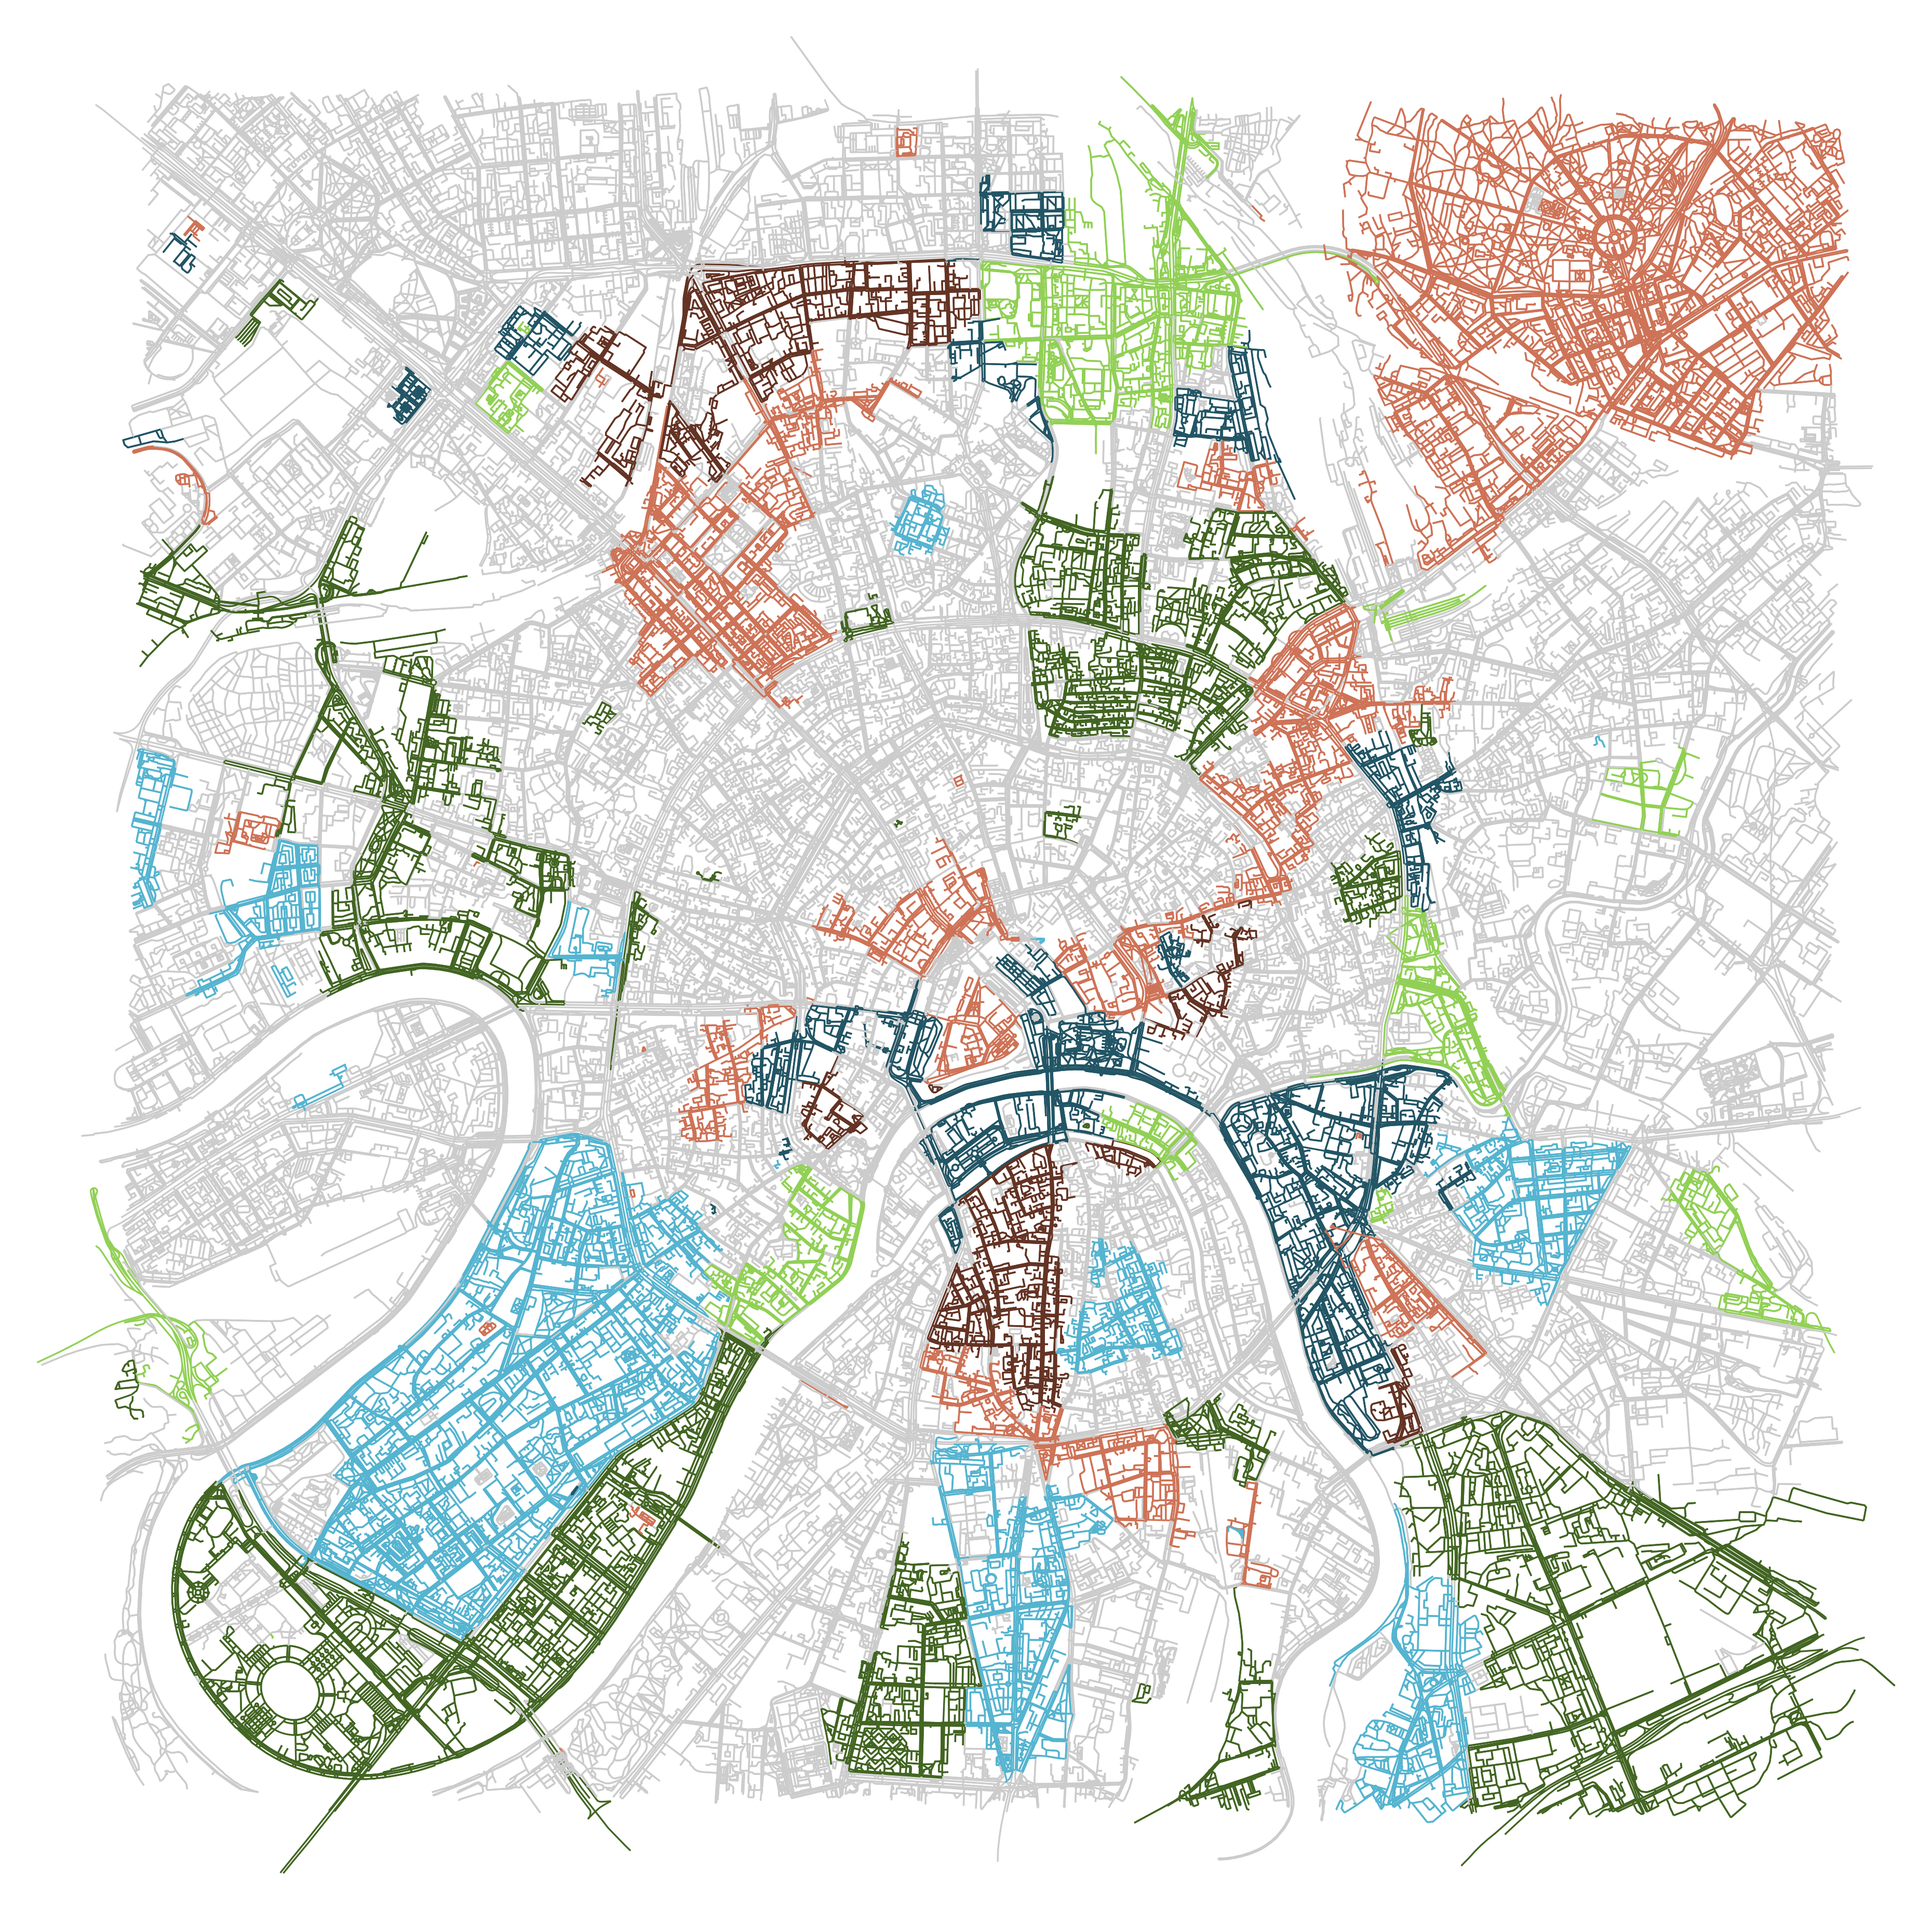
\includegraphics[width=0.85\linewidth]{maps/Moscow.png} \\[-0.5ex]
\bottomrule
\end{tabularx}
\end{adjustwidth}
\end{table}

\begin{table}[H]
\caption{Geometrical group of cities considered in this study: Medellin (Colombia), Palmanova (Italy), Dubai (UAE), and Canberra (Australia). For each city, the table provides basic data, the UMAP+HDBSCAN embedding, and the colored map projection at the chosen scale, together with the taxonomy label from Lima’s classification.}
\label{table_geometrical_embeddings}

\begin{adjustwidth}{-\extralength}{0cm}
%\centering %% If there is a figure in wide page, please release command \centering
\begin{tabularx}{\fulllength}{>{\raggedright\arraybackslash}X m{6cm}<{\centering}m{6cm}<{\centering}}
\toprule
\textbf{City Info} & \multicolumn{1}{c}{\textbf{Embedding}} & \multicolumn{1}{c}{\textbf{Map}} \\
\midrule
\textbf{{Medellin}} \newline Country: Colombia \newline Lat/Lon: (6.2518, $-$75.5836) \newline Scale: 10 km \newline Group: Geometrical \newline Taxonomy Label: \newline Arc Diagram &
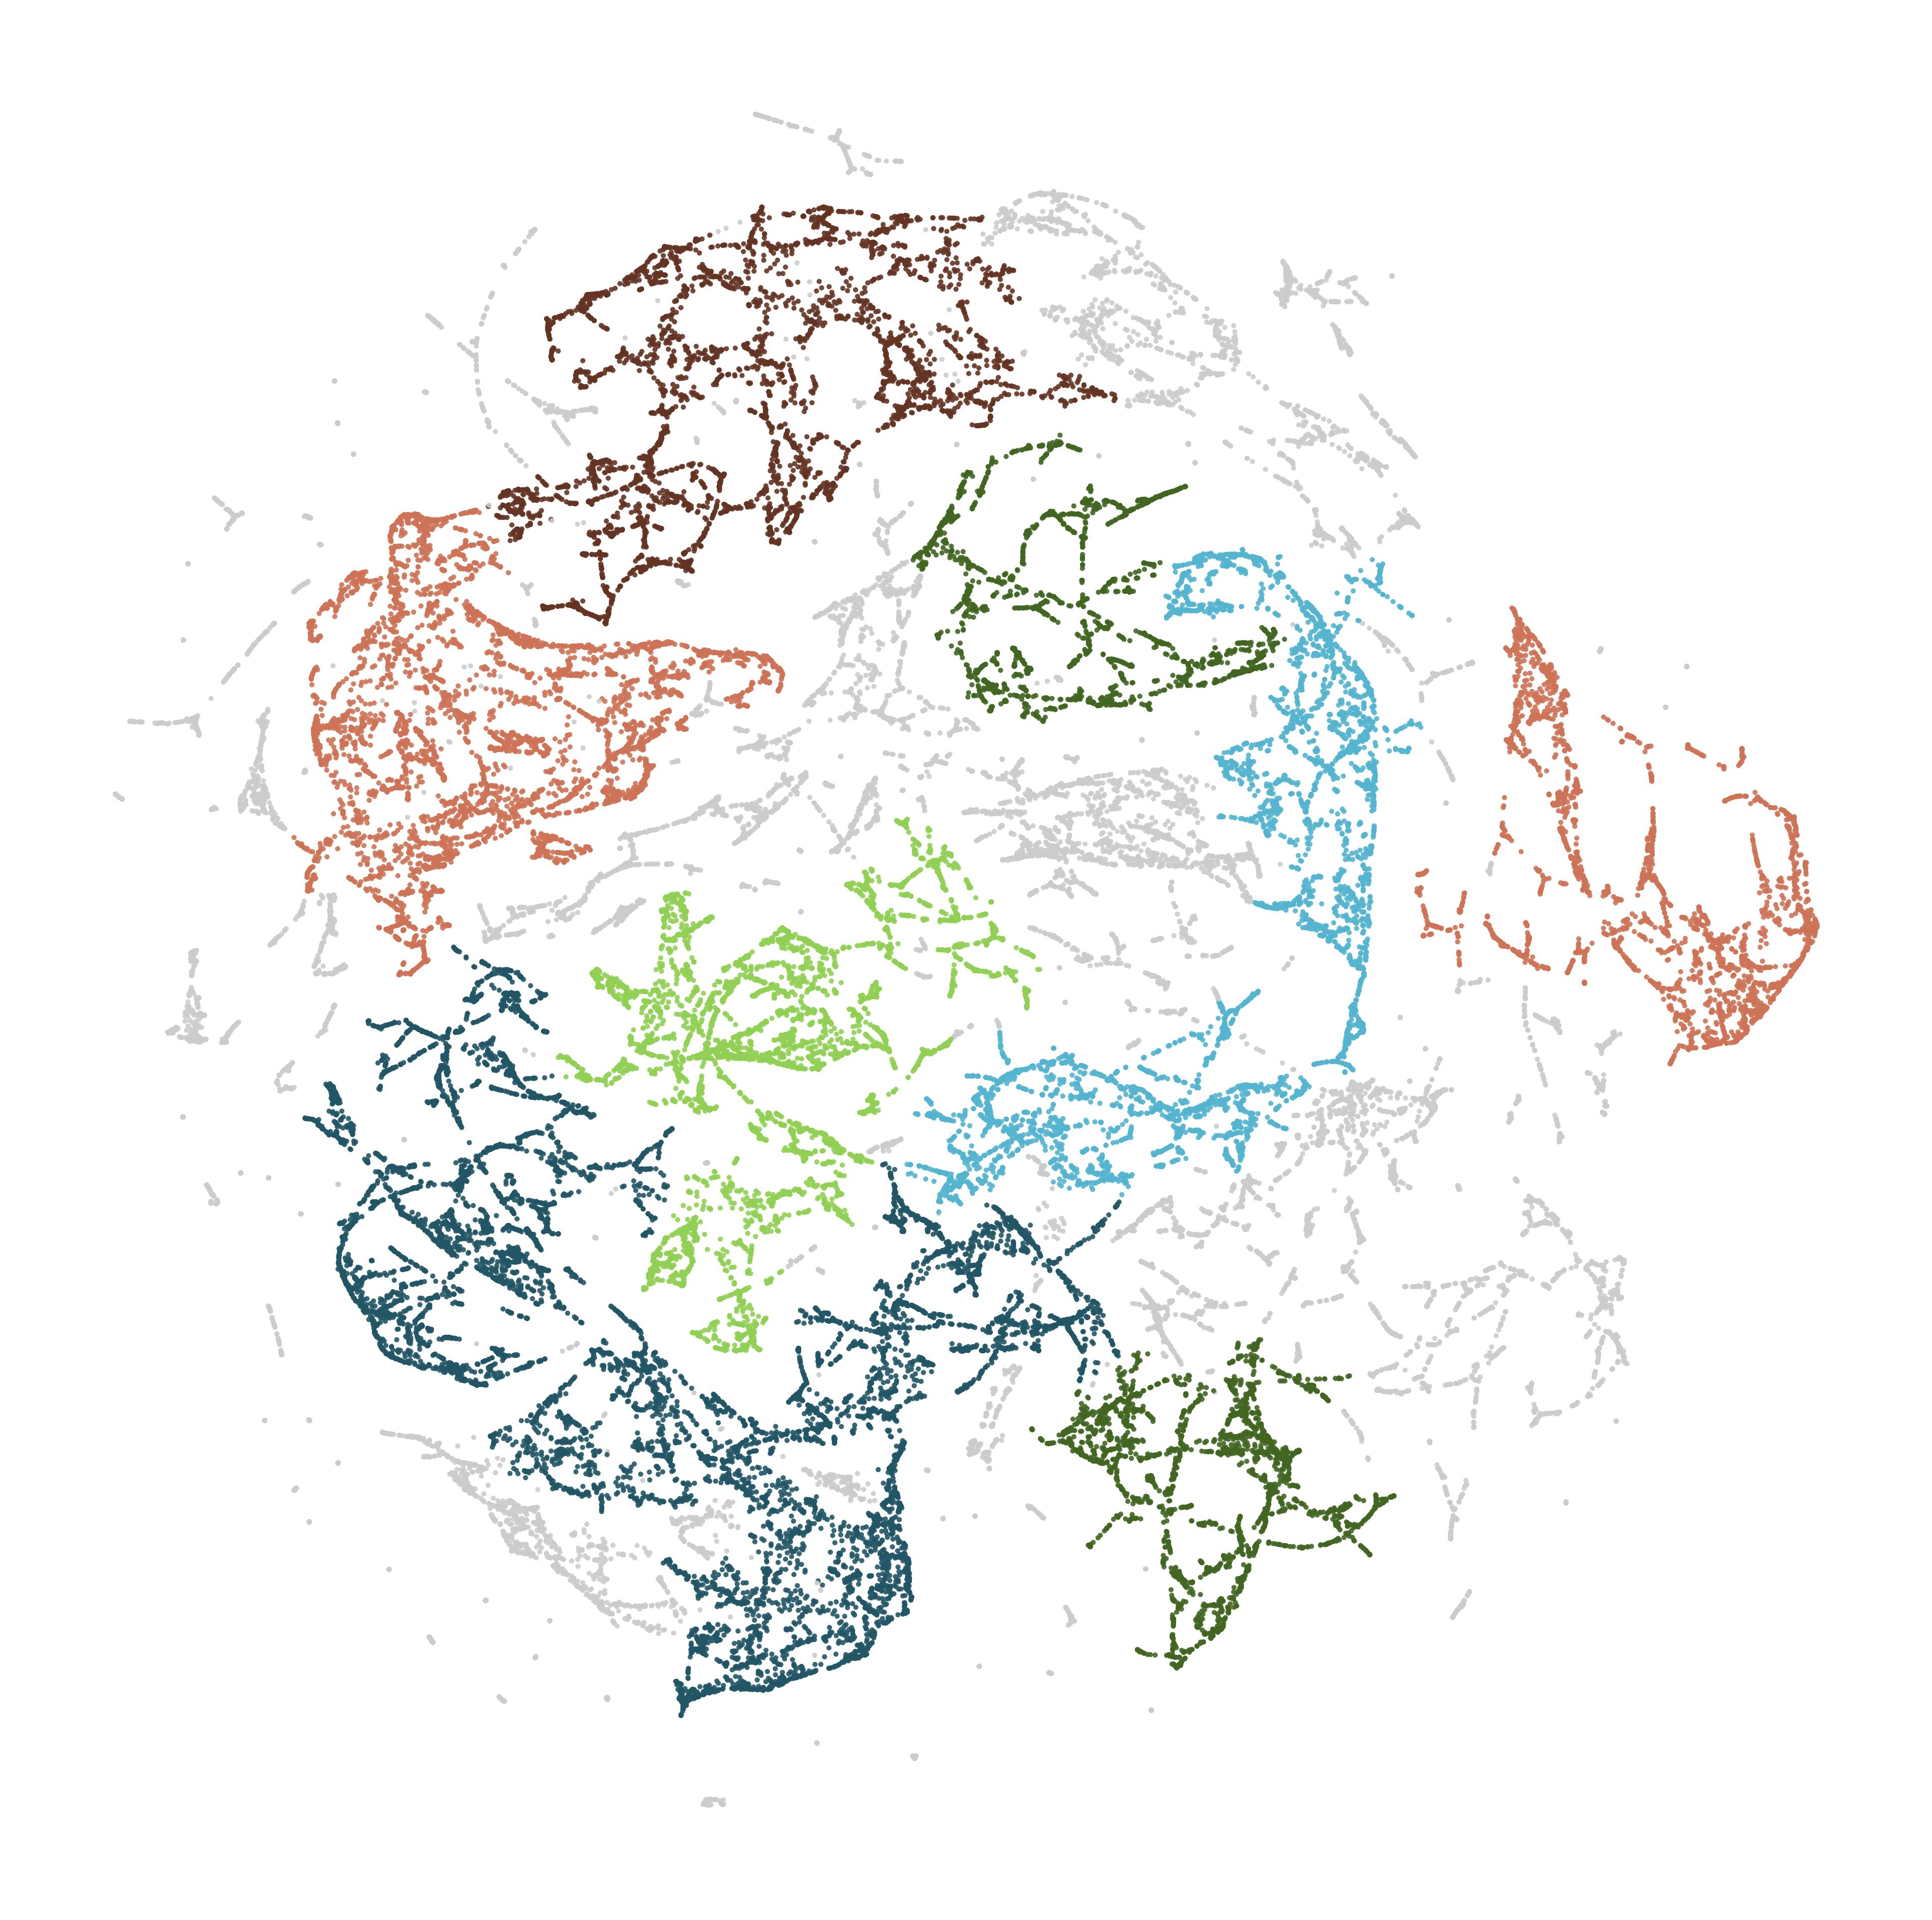
\includegraphics[width=0.85\linewidth]{clusters/Medellin.jpg} &
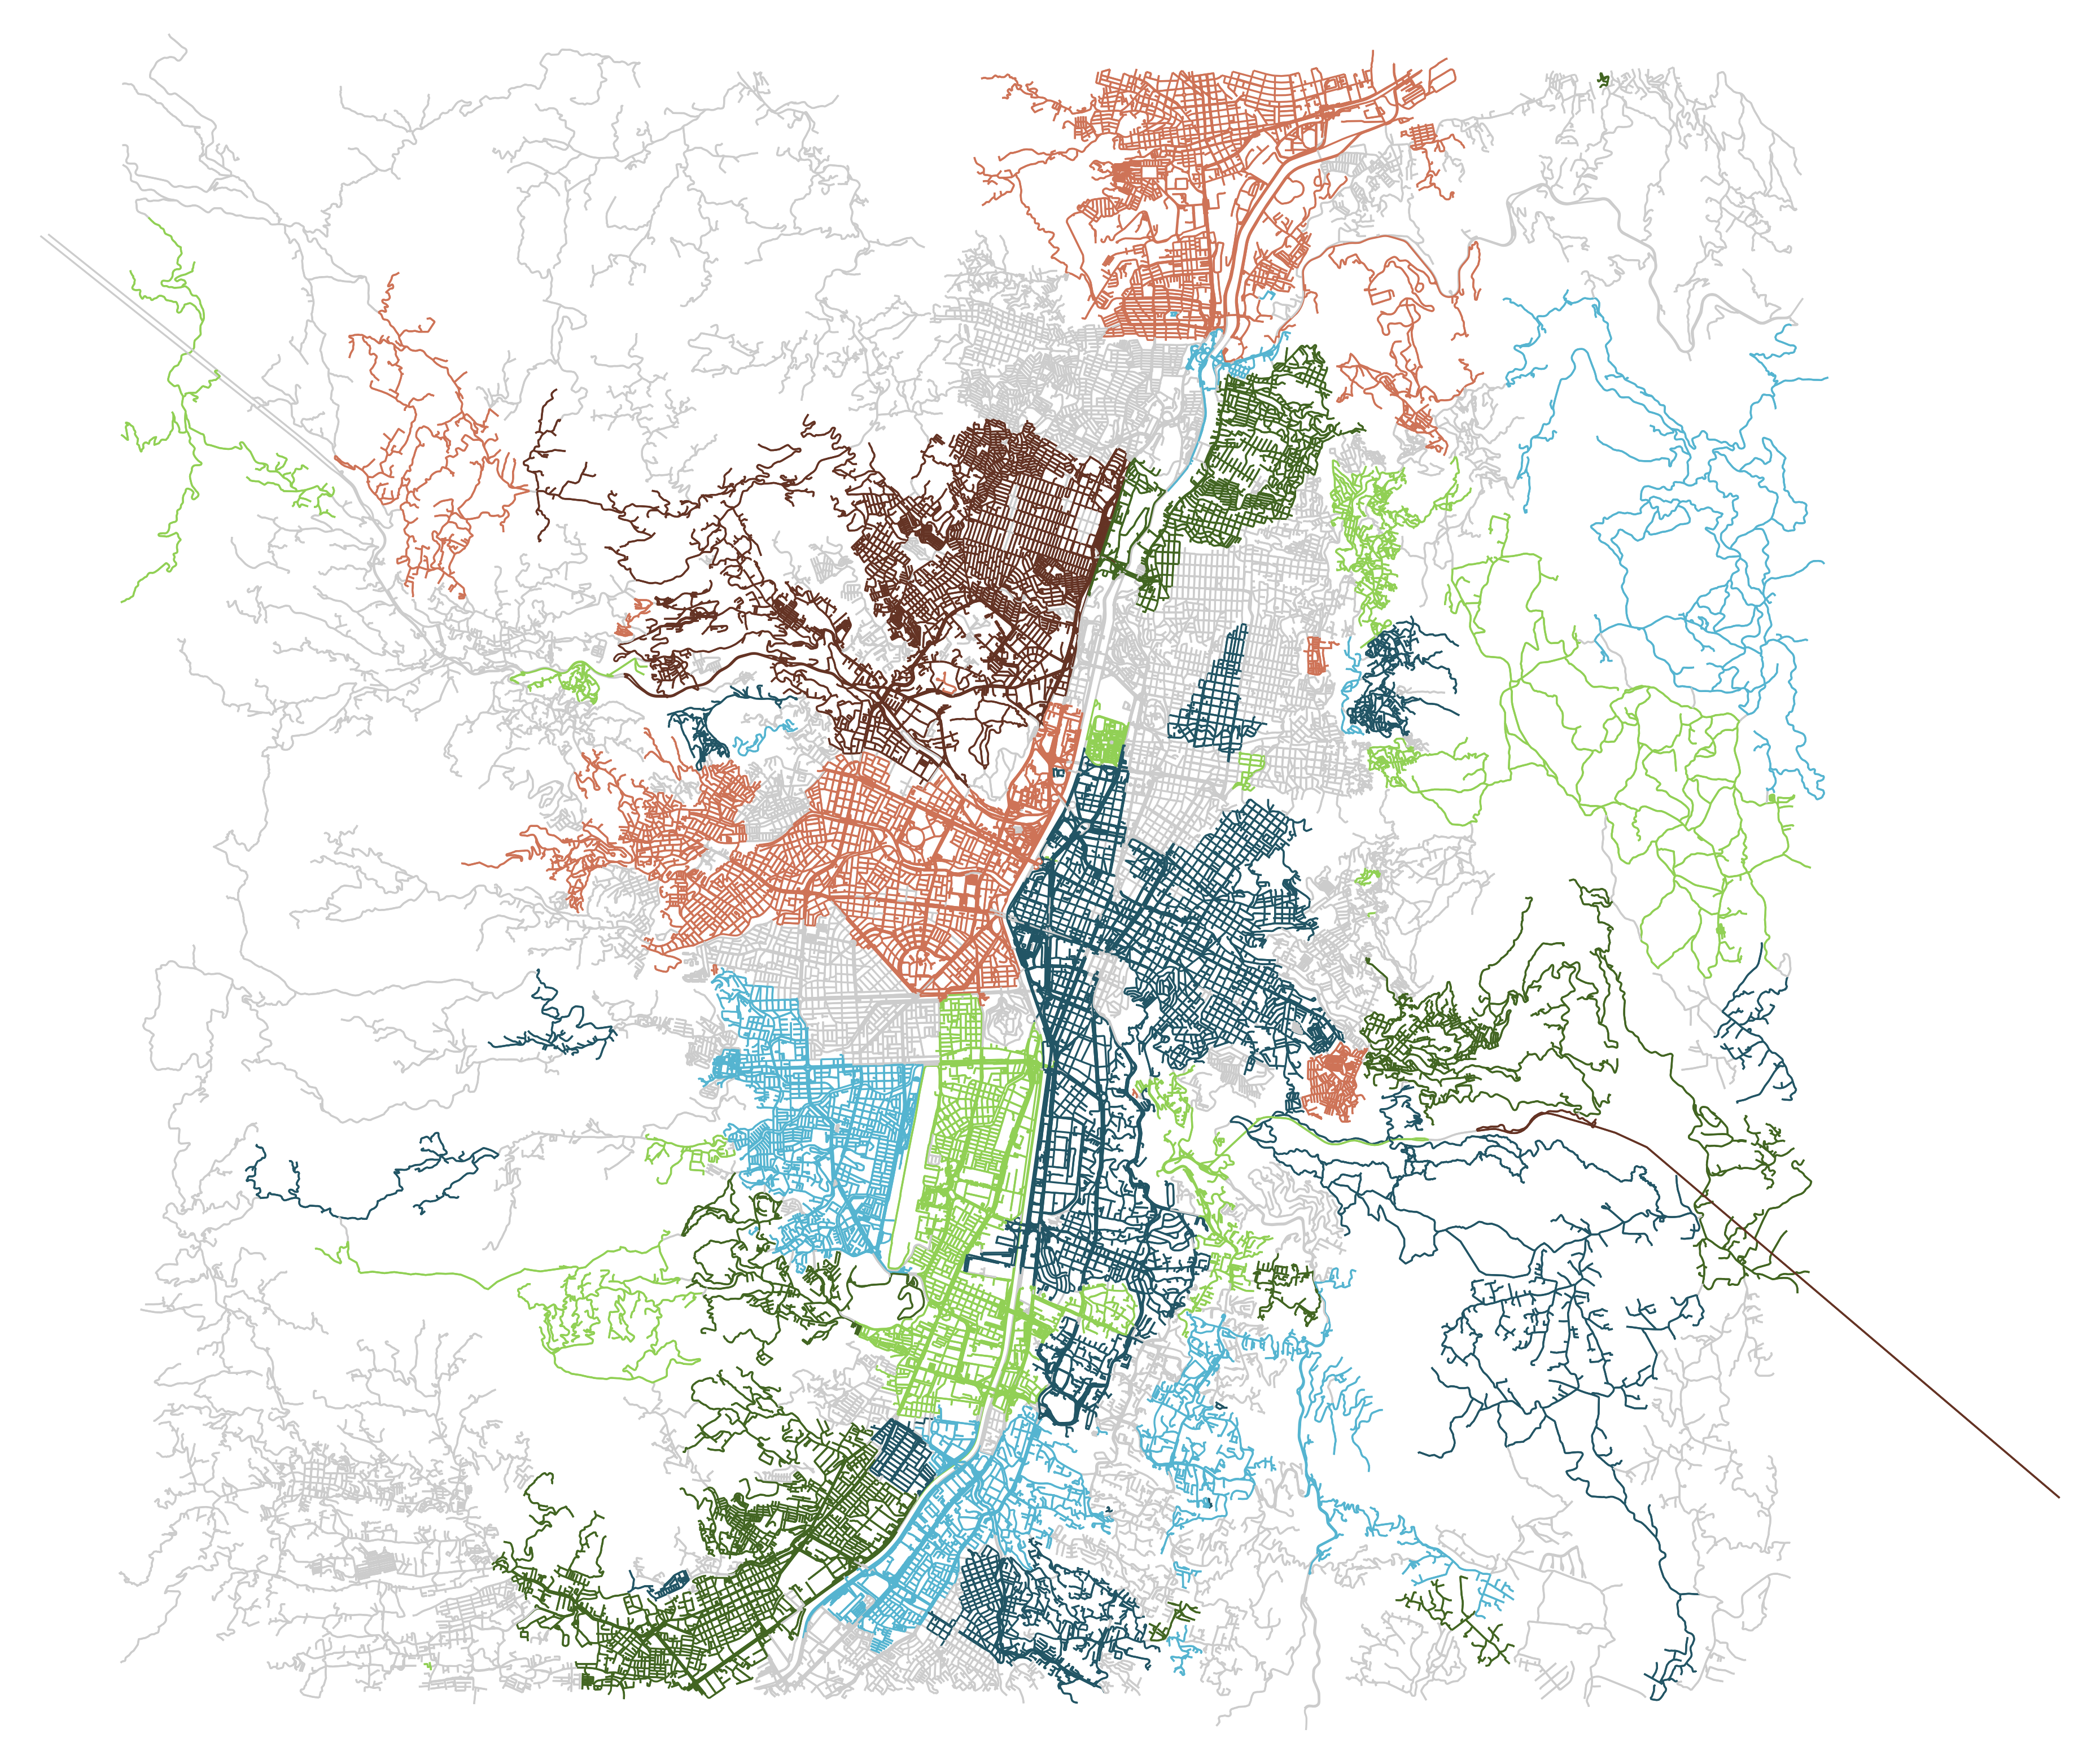
\includegraphics[width=0.85\linewidth]{maps/Medellin.png} \\[-3ex]
\midrule
\textbf{{Palmanova}} \newline Country: Italy \newline Lat/Lon: (45.9061, 13.3095) \newline Scale: 1 km \newline Group: Geometrical \newline Taxonomy Label: \newline Radial Convergence &
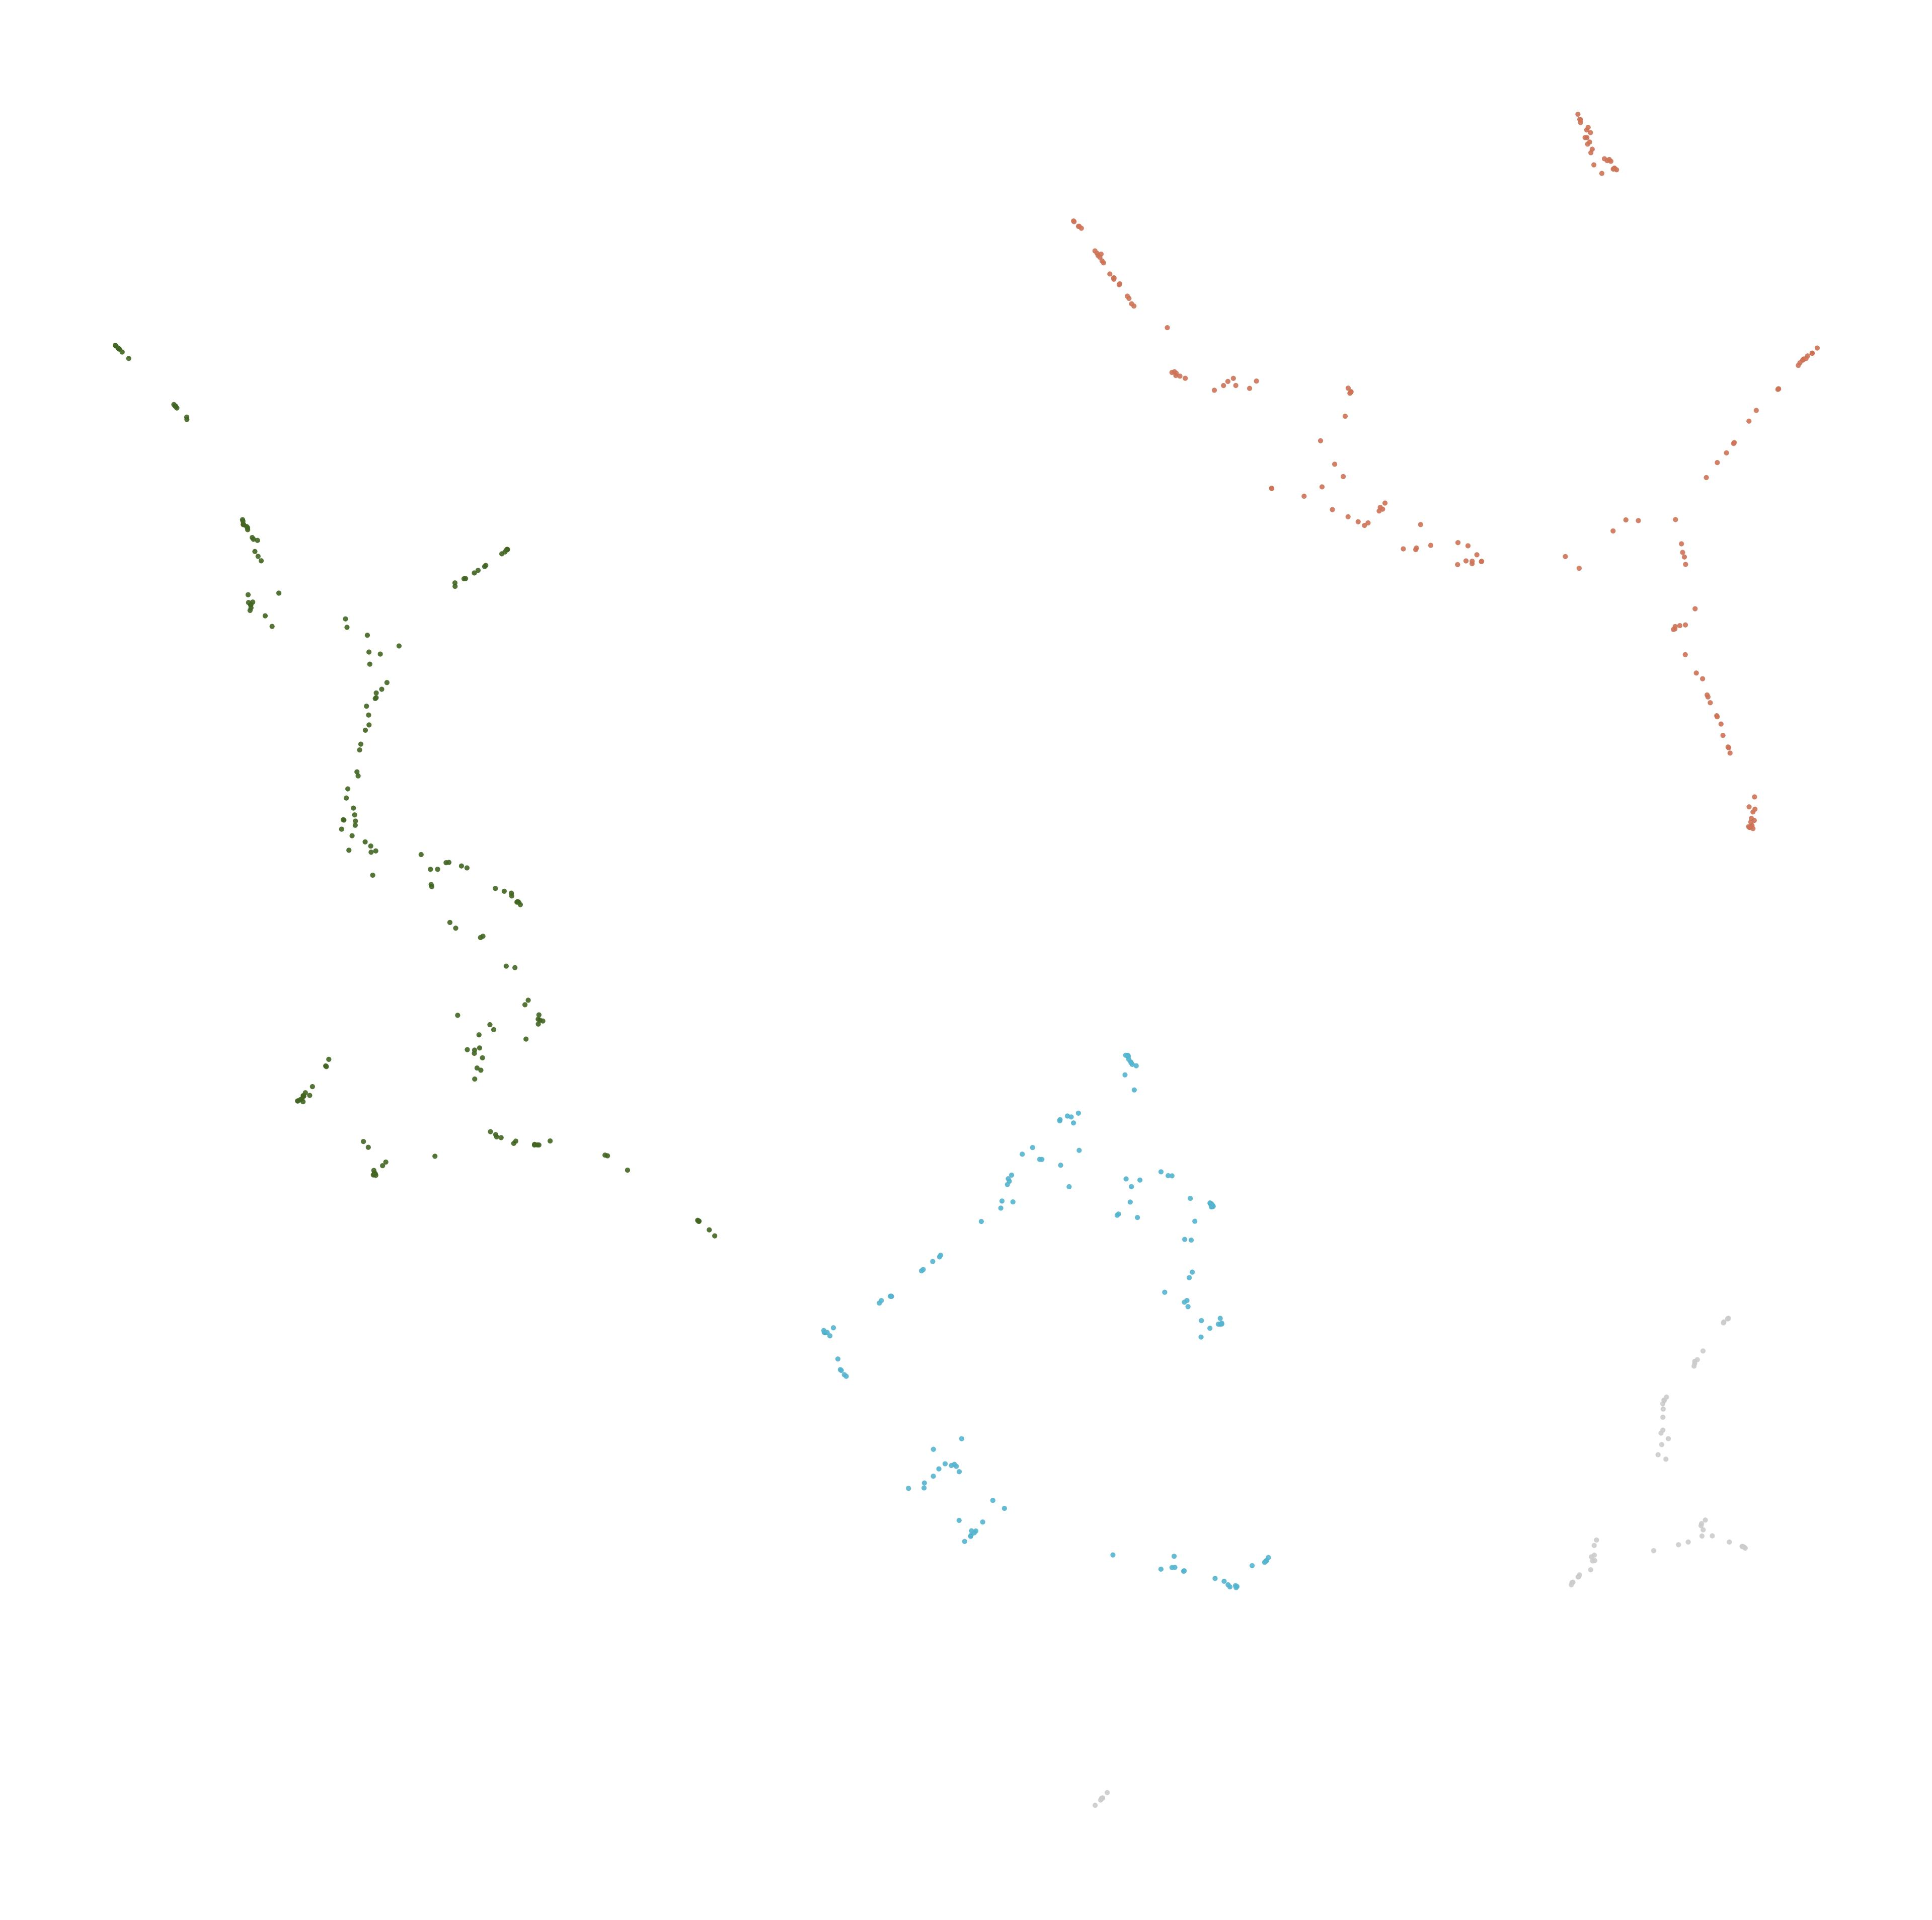
\includegraphics[width=0.85\linewidth]{clusters/Palmanova.jpg} &
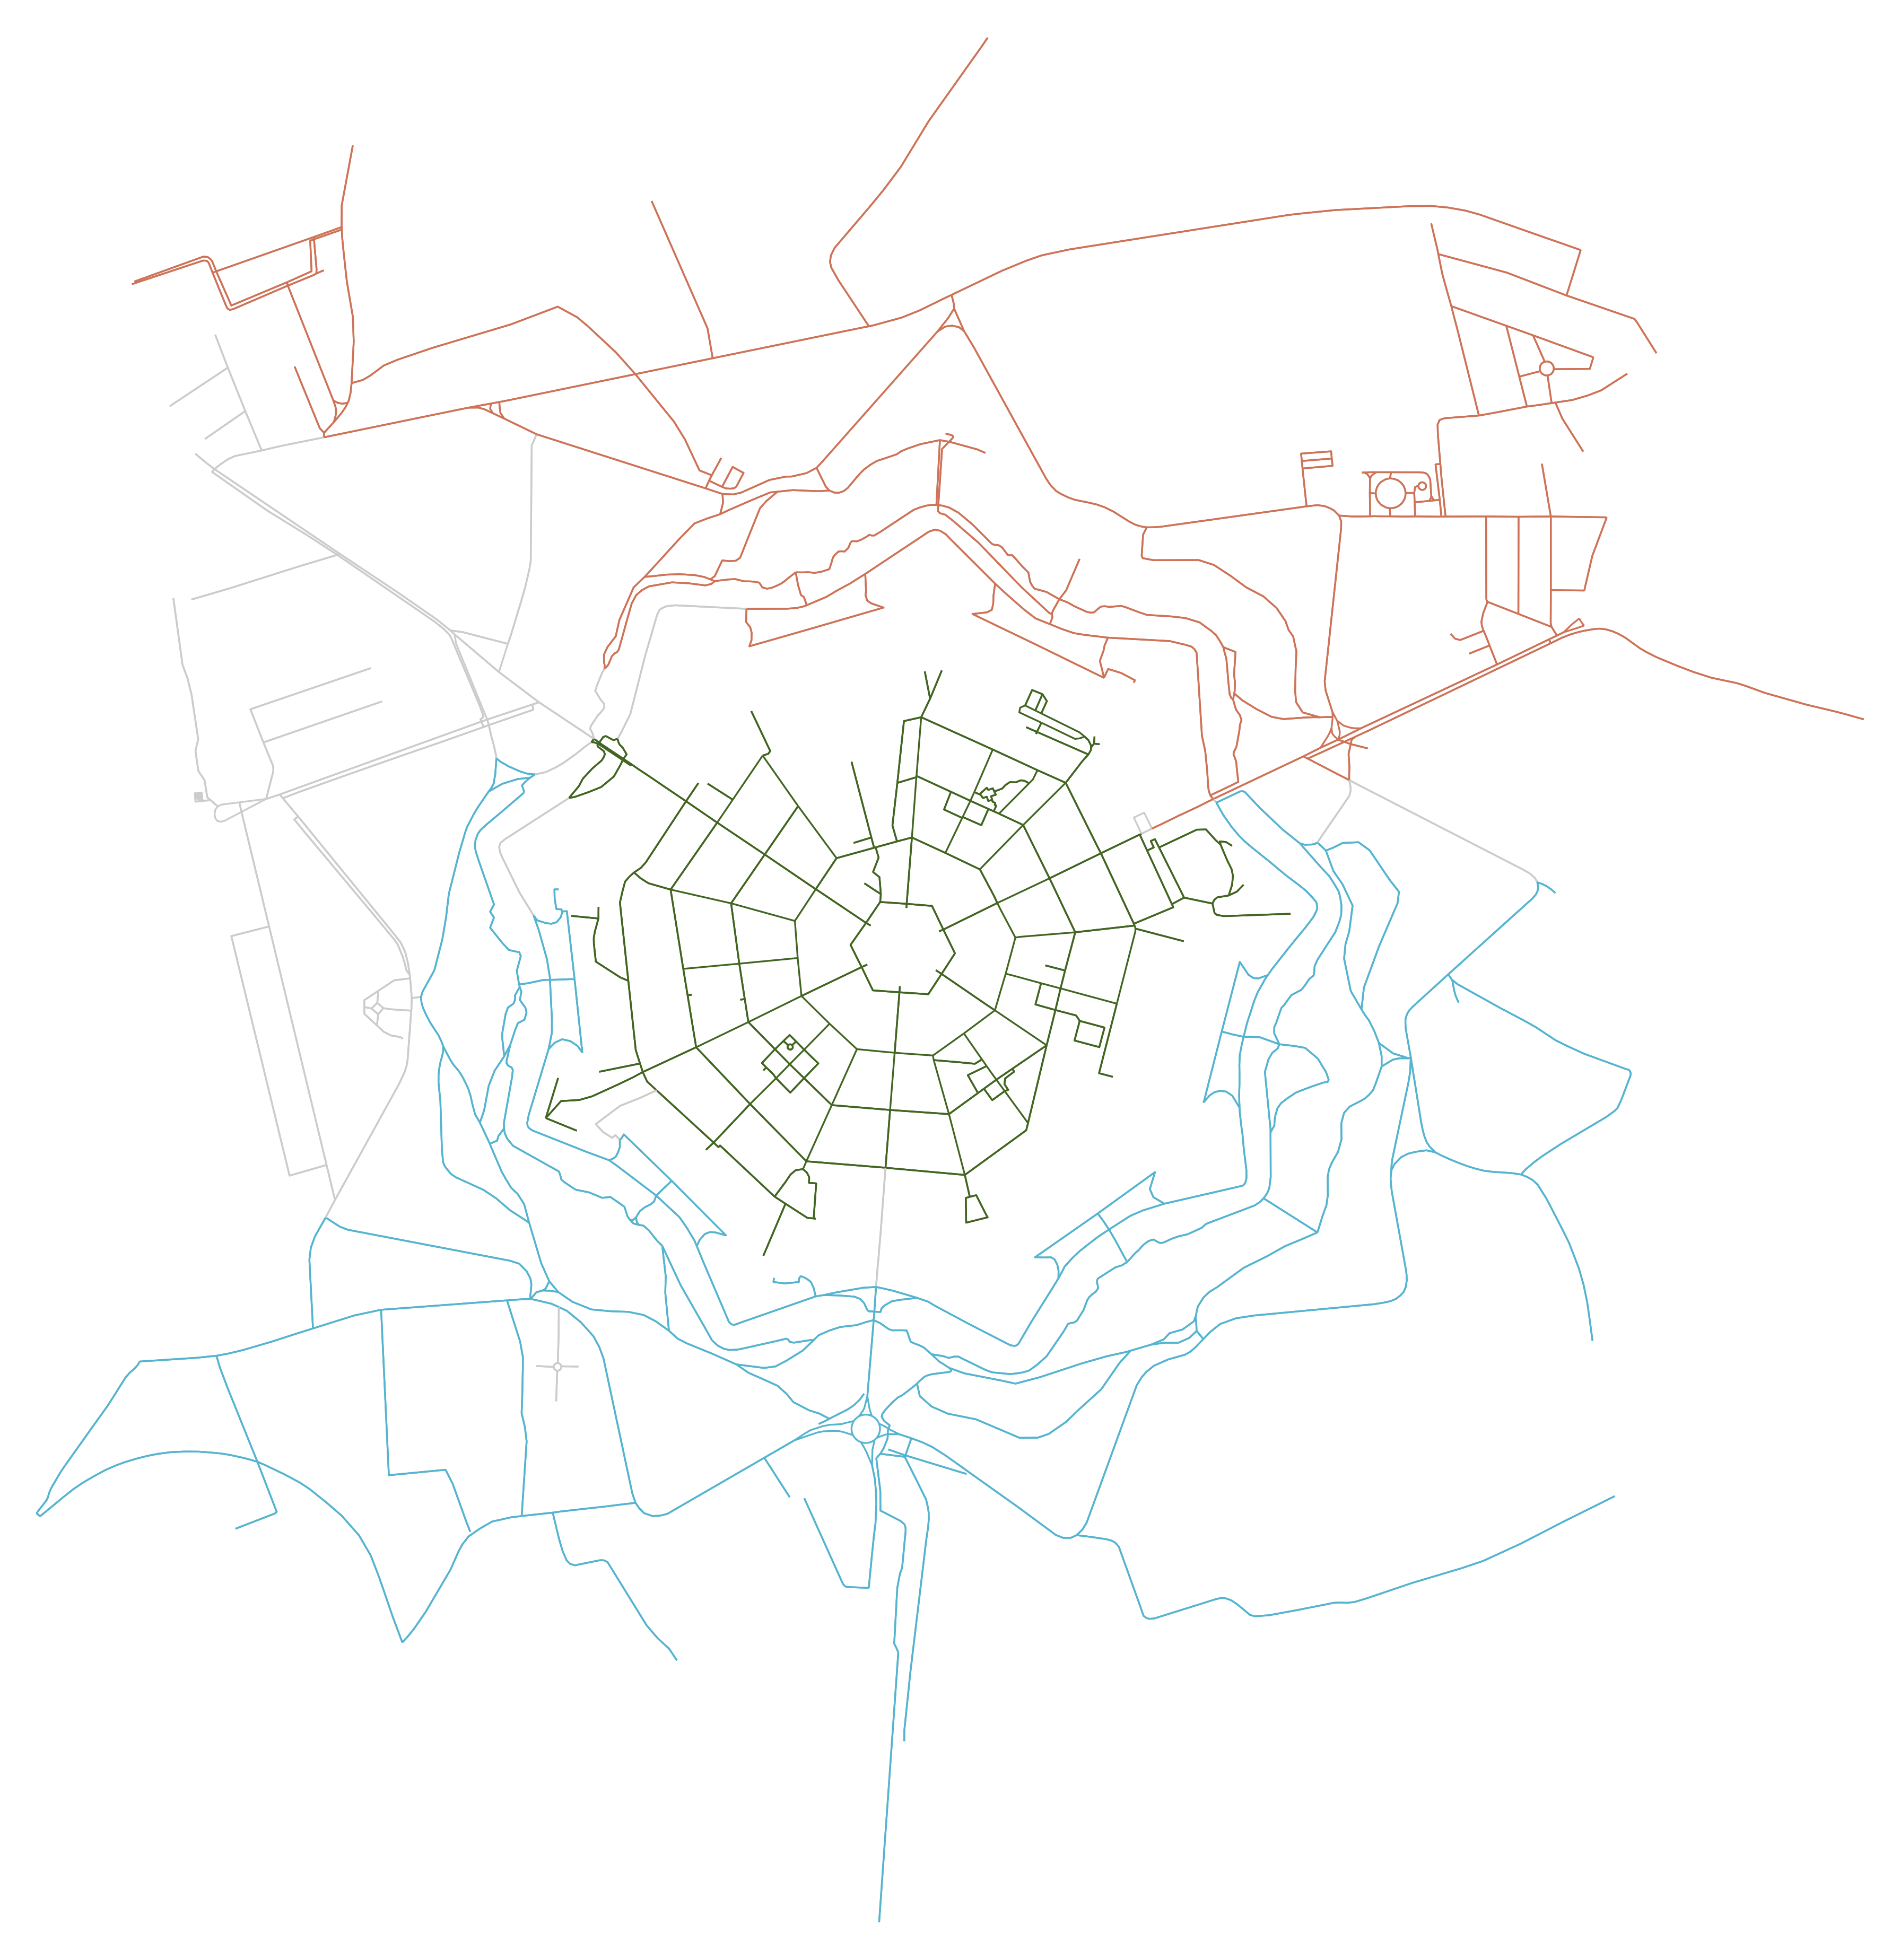
\includegraphics[width=0.85\linewidth]{maps/Palmanova.png} \\[-0.5ex]
\midrule
\textbf{{Dubai}} \newline Country: United Arab Emirates \newline Lat/Lon: (25.0565, 55.2070) \newline Scale: 1 km \newline Group: Geometrical \newline Taxonomy Label: \newline Segmented Radial Convergence &
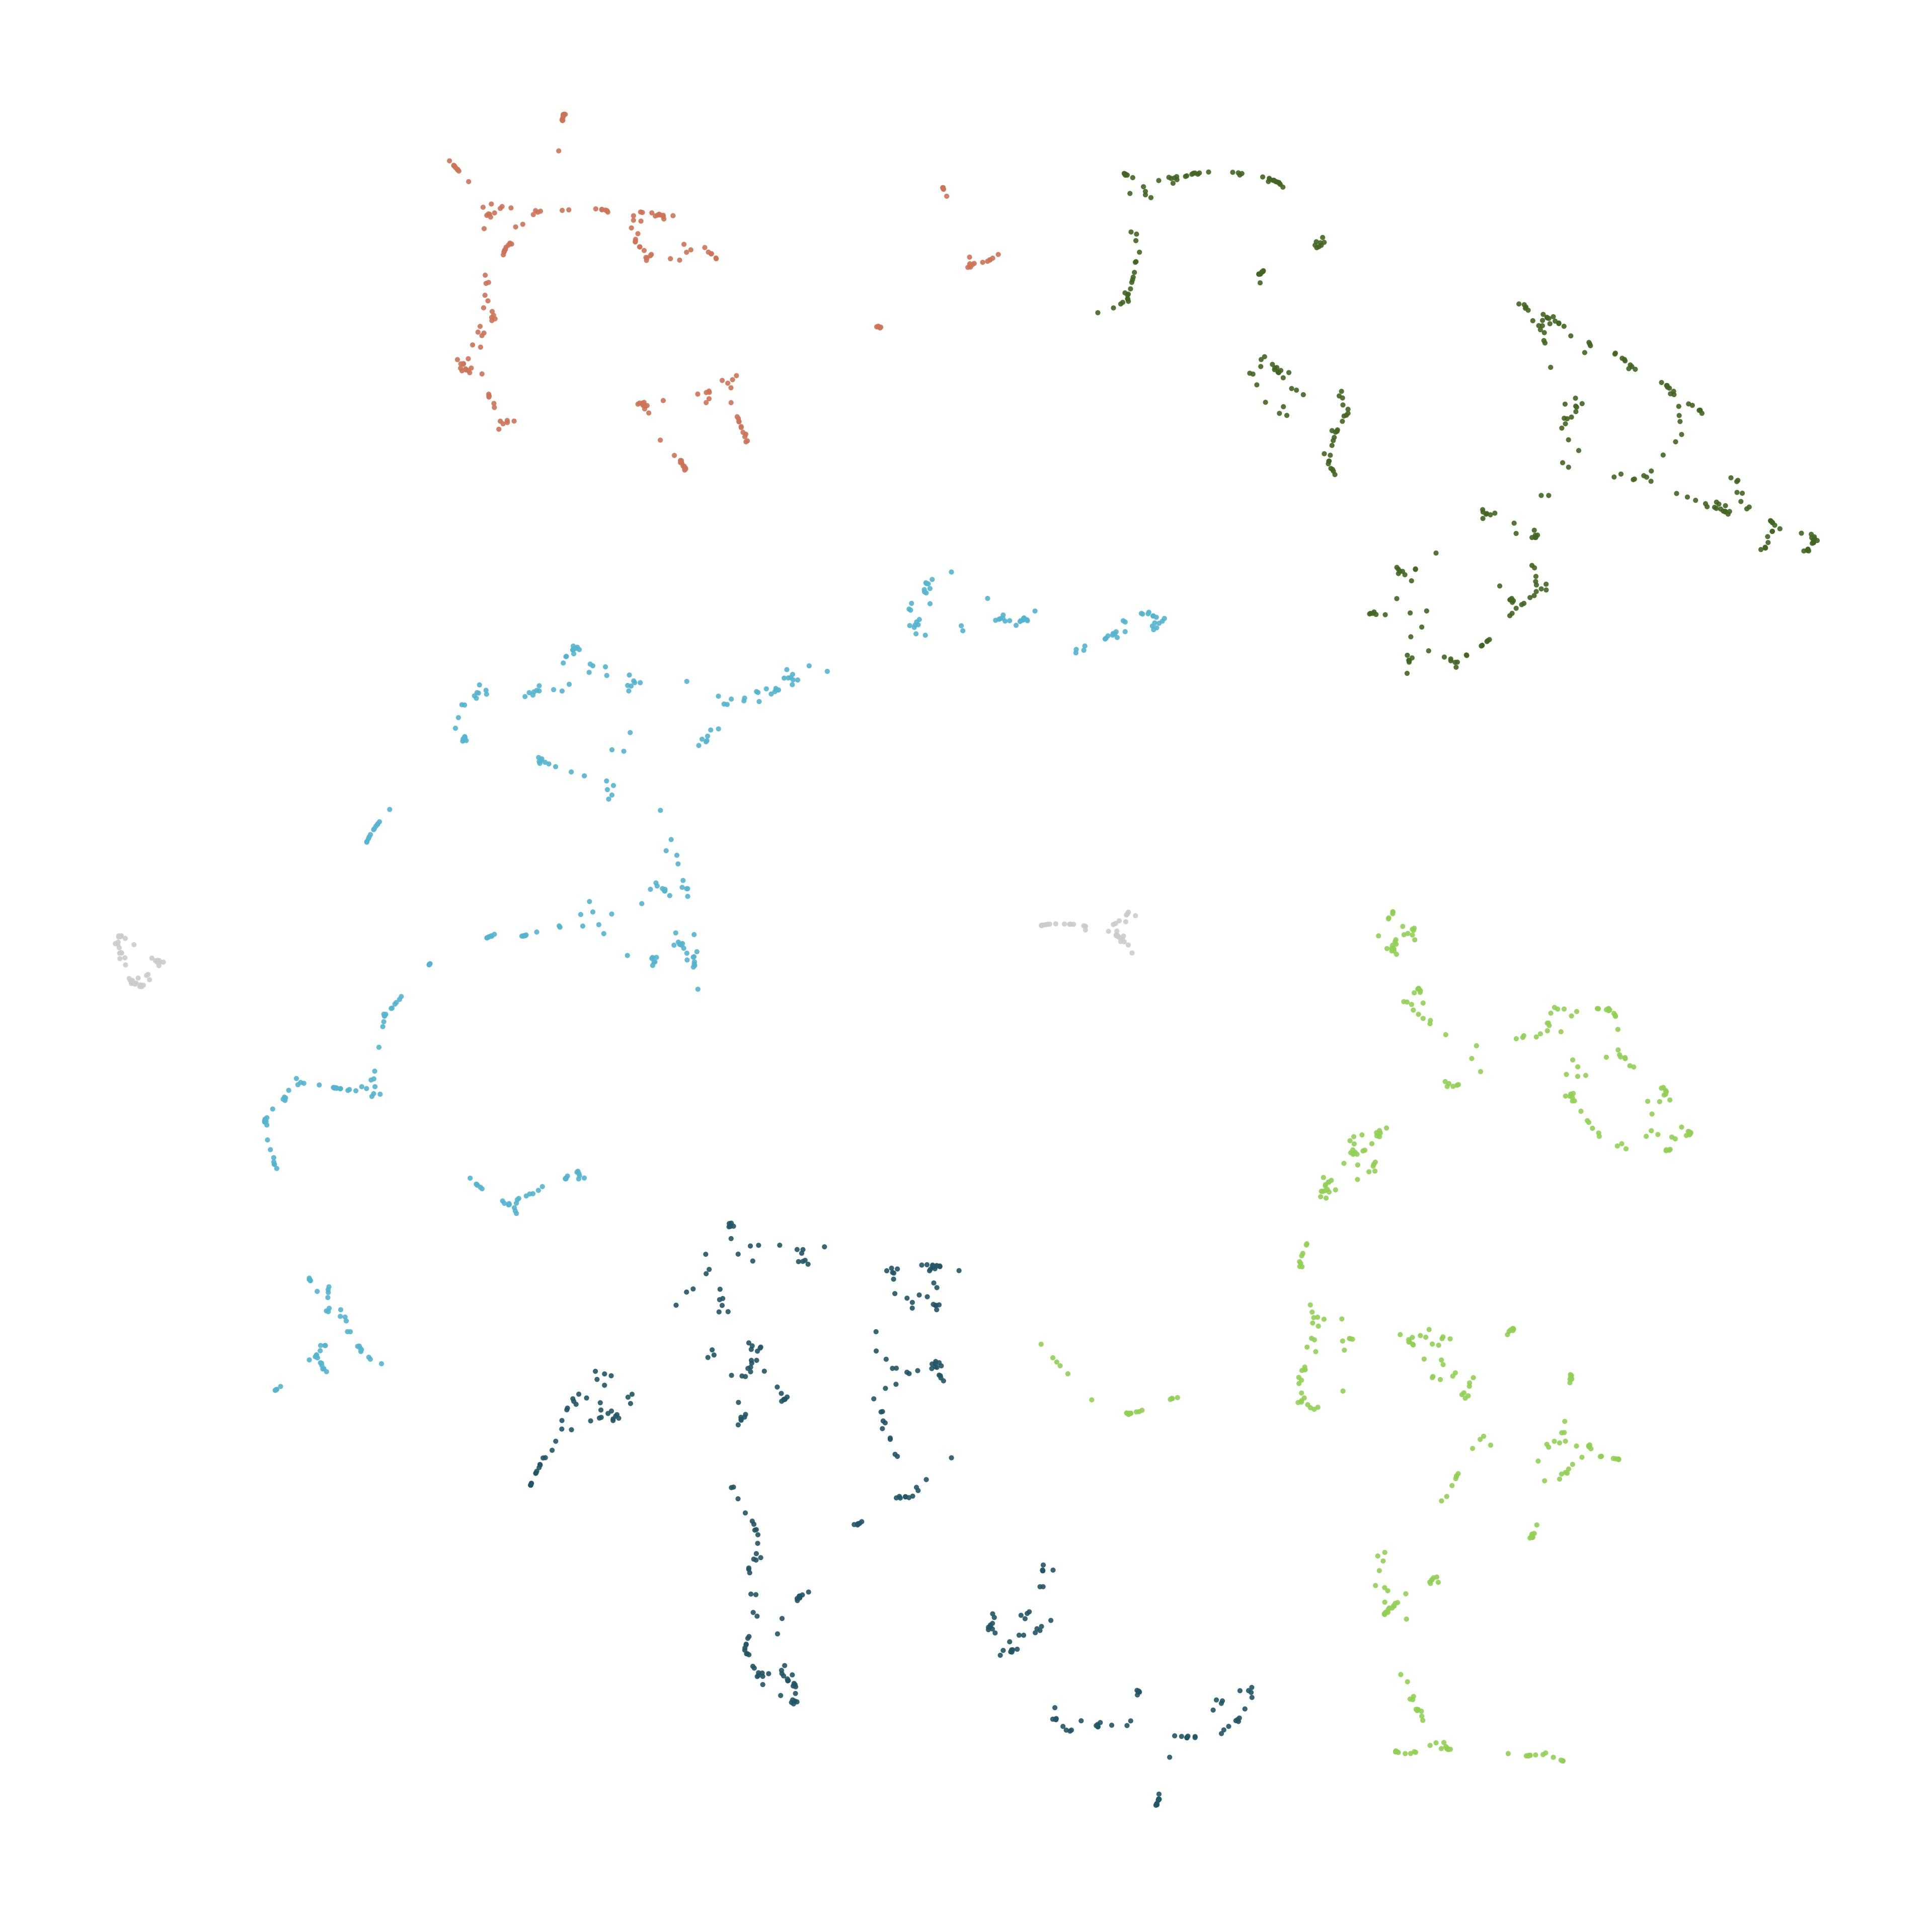
\includegraphics[width=0.85\linewidth]{clusters/Dubai.jpg} &
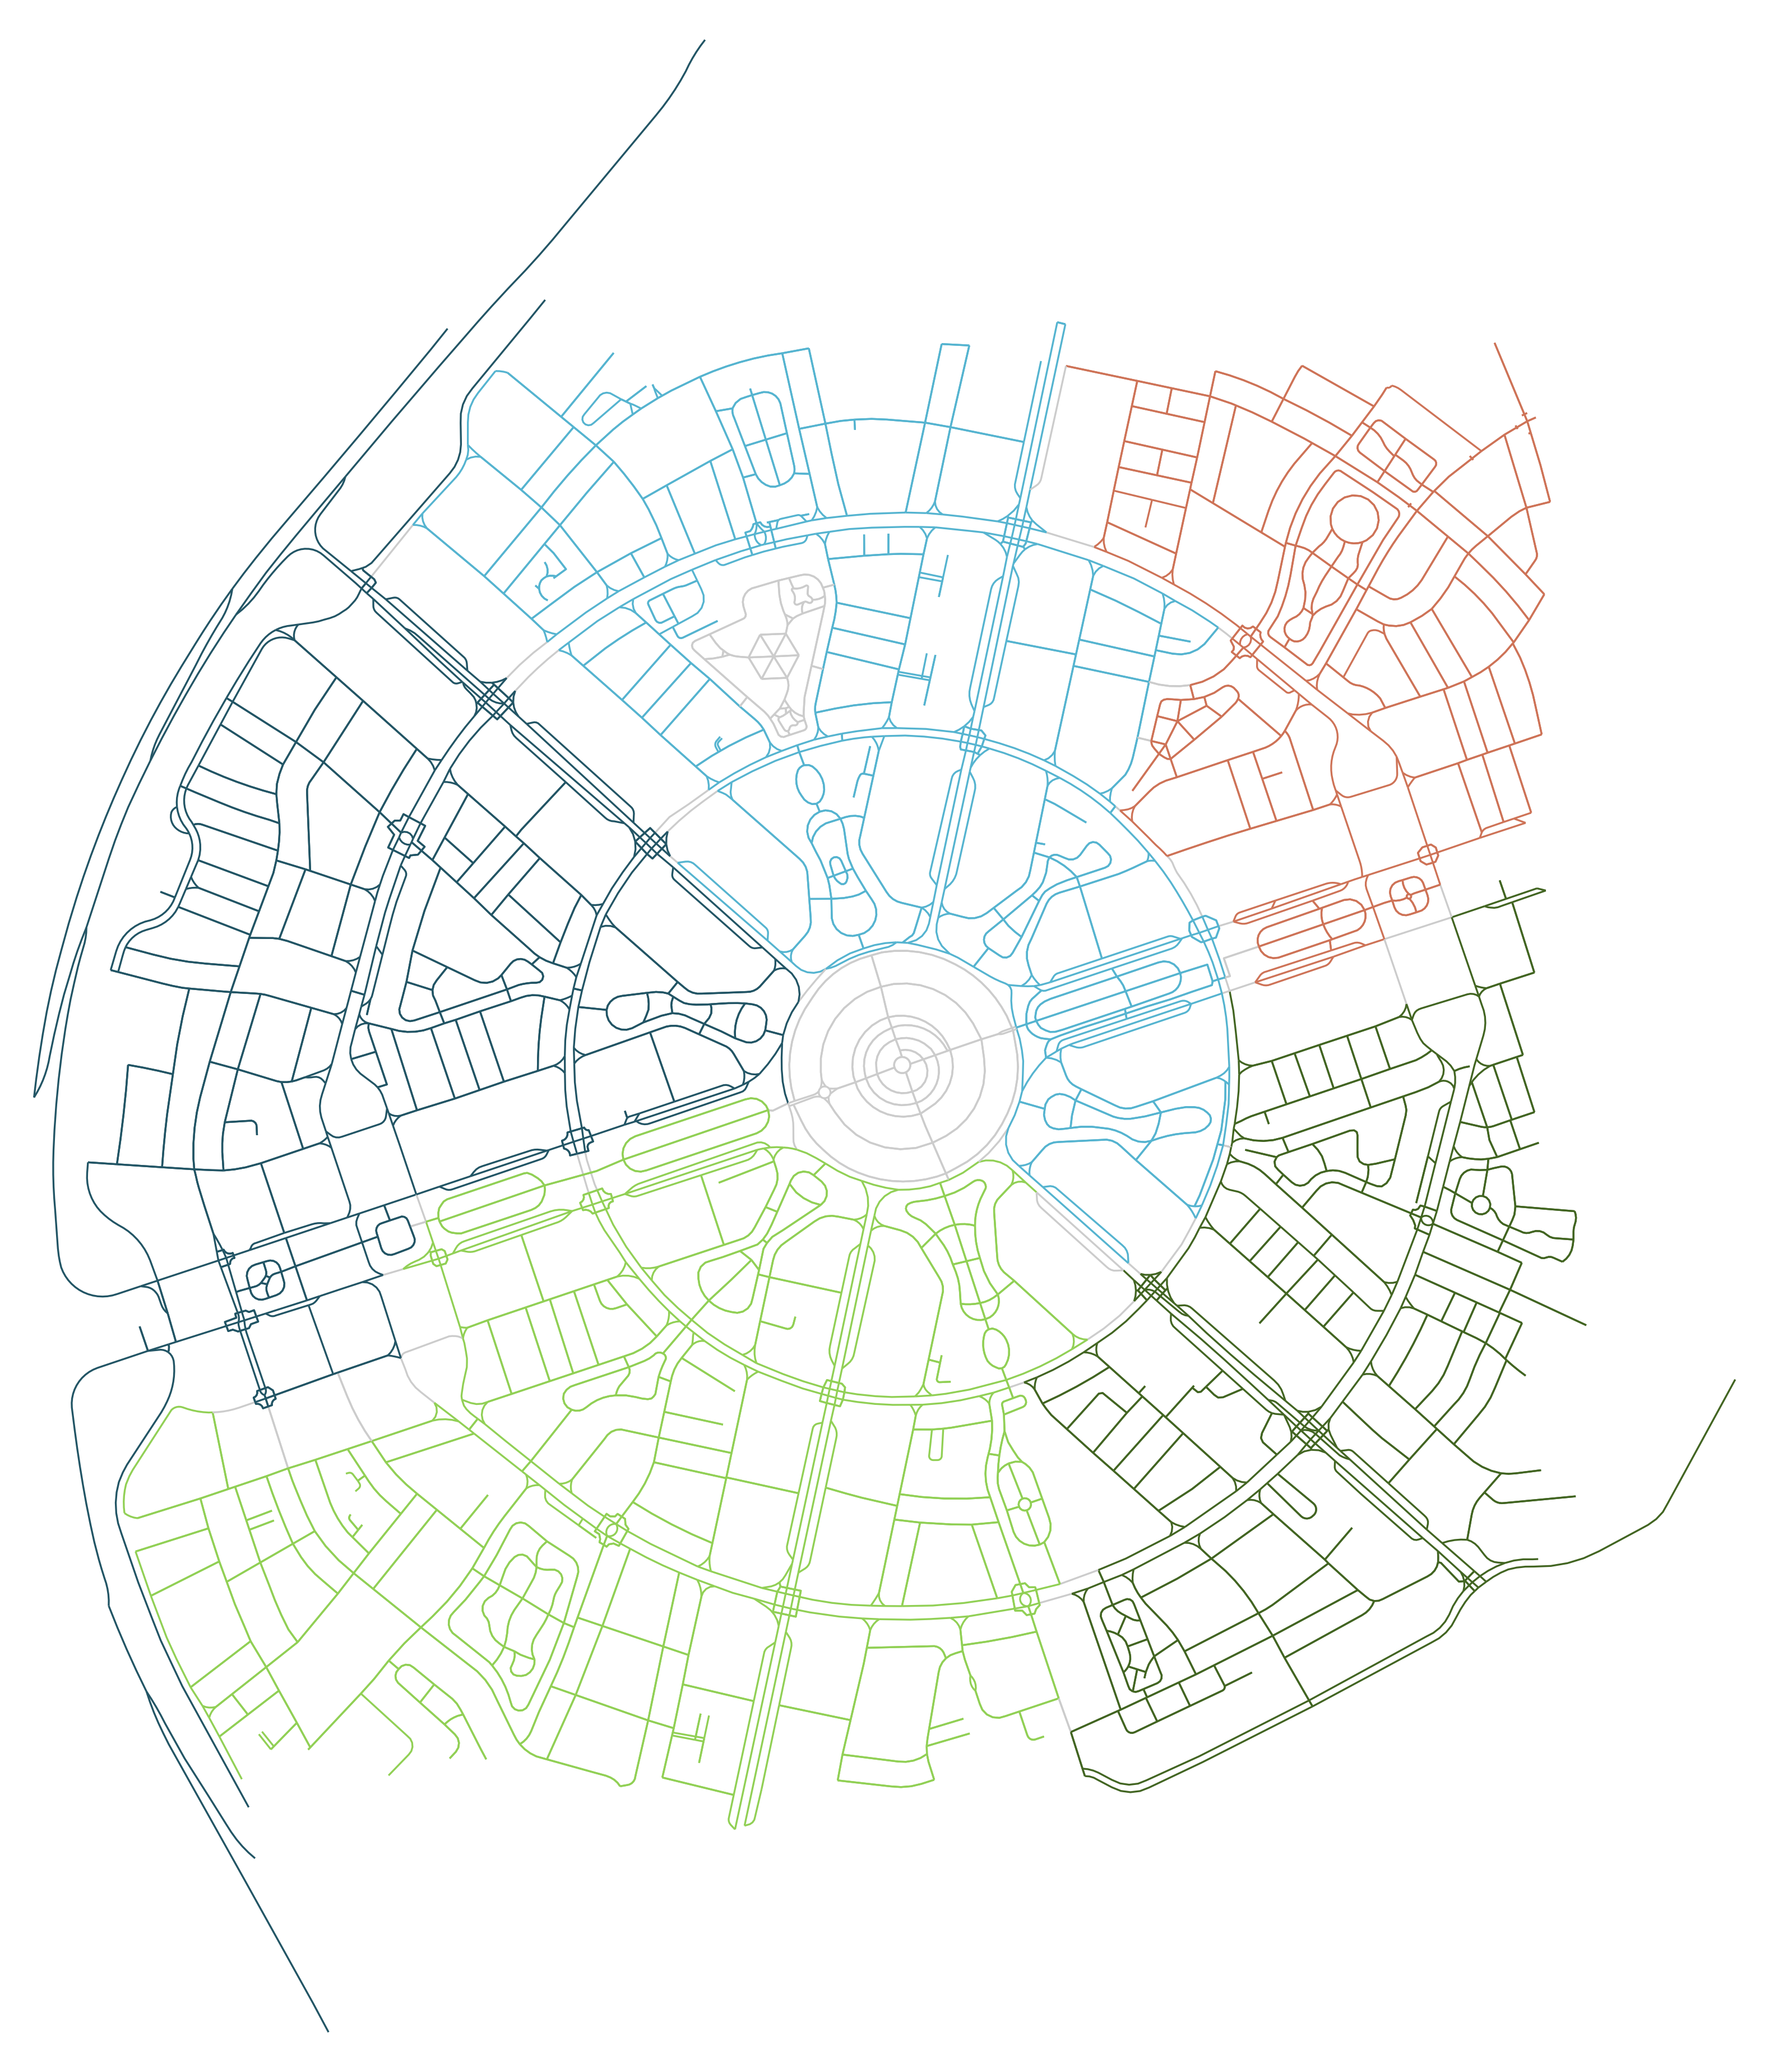
\includegraphics[width=0.85\linewidth]{maps/Dubai.png} \\[-0.5ex]
\midrule
\textbf{{Canberra}} \newline Country: Australia \newline Lat/Lon: ($-$35.3082, 149.1244) \newline Scale: 3.5 km \newline Group: Geometrical \newline Taxonomy Label: \newline Centralized Ring &
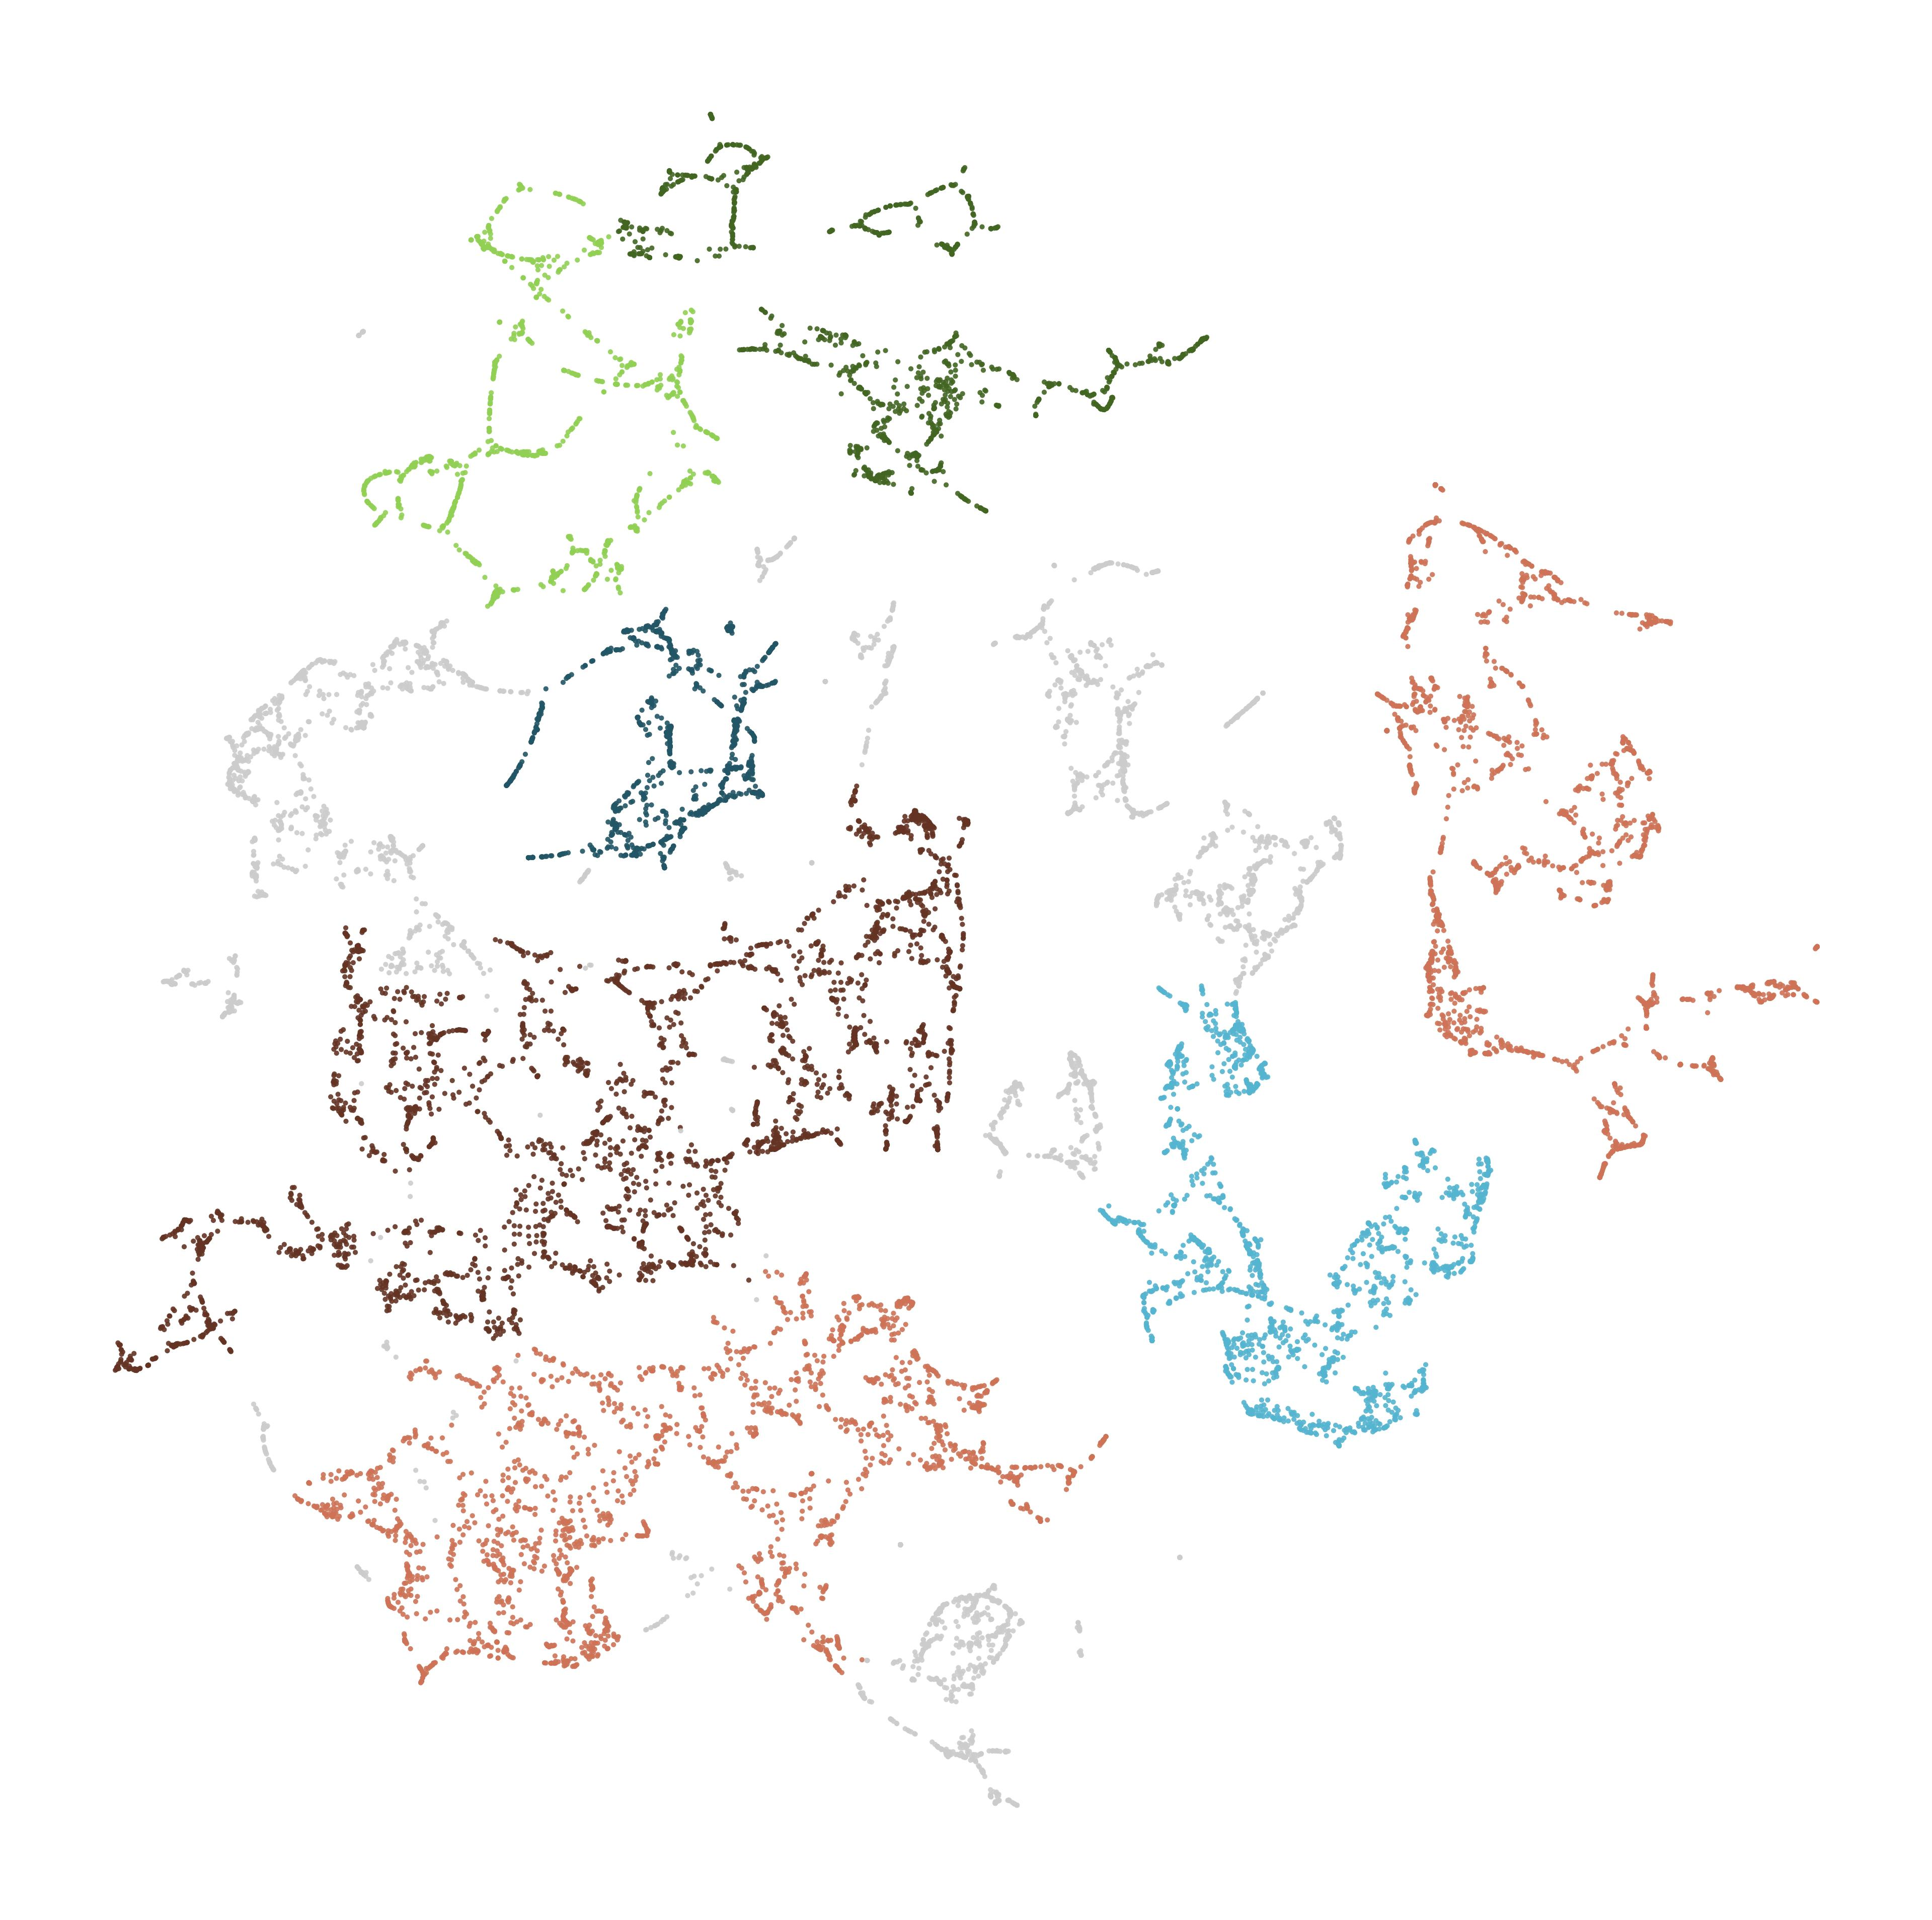
\includegraphics[width=0.85\linewidth]{clusters/Canberra.jpg} &
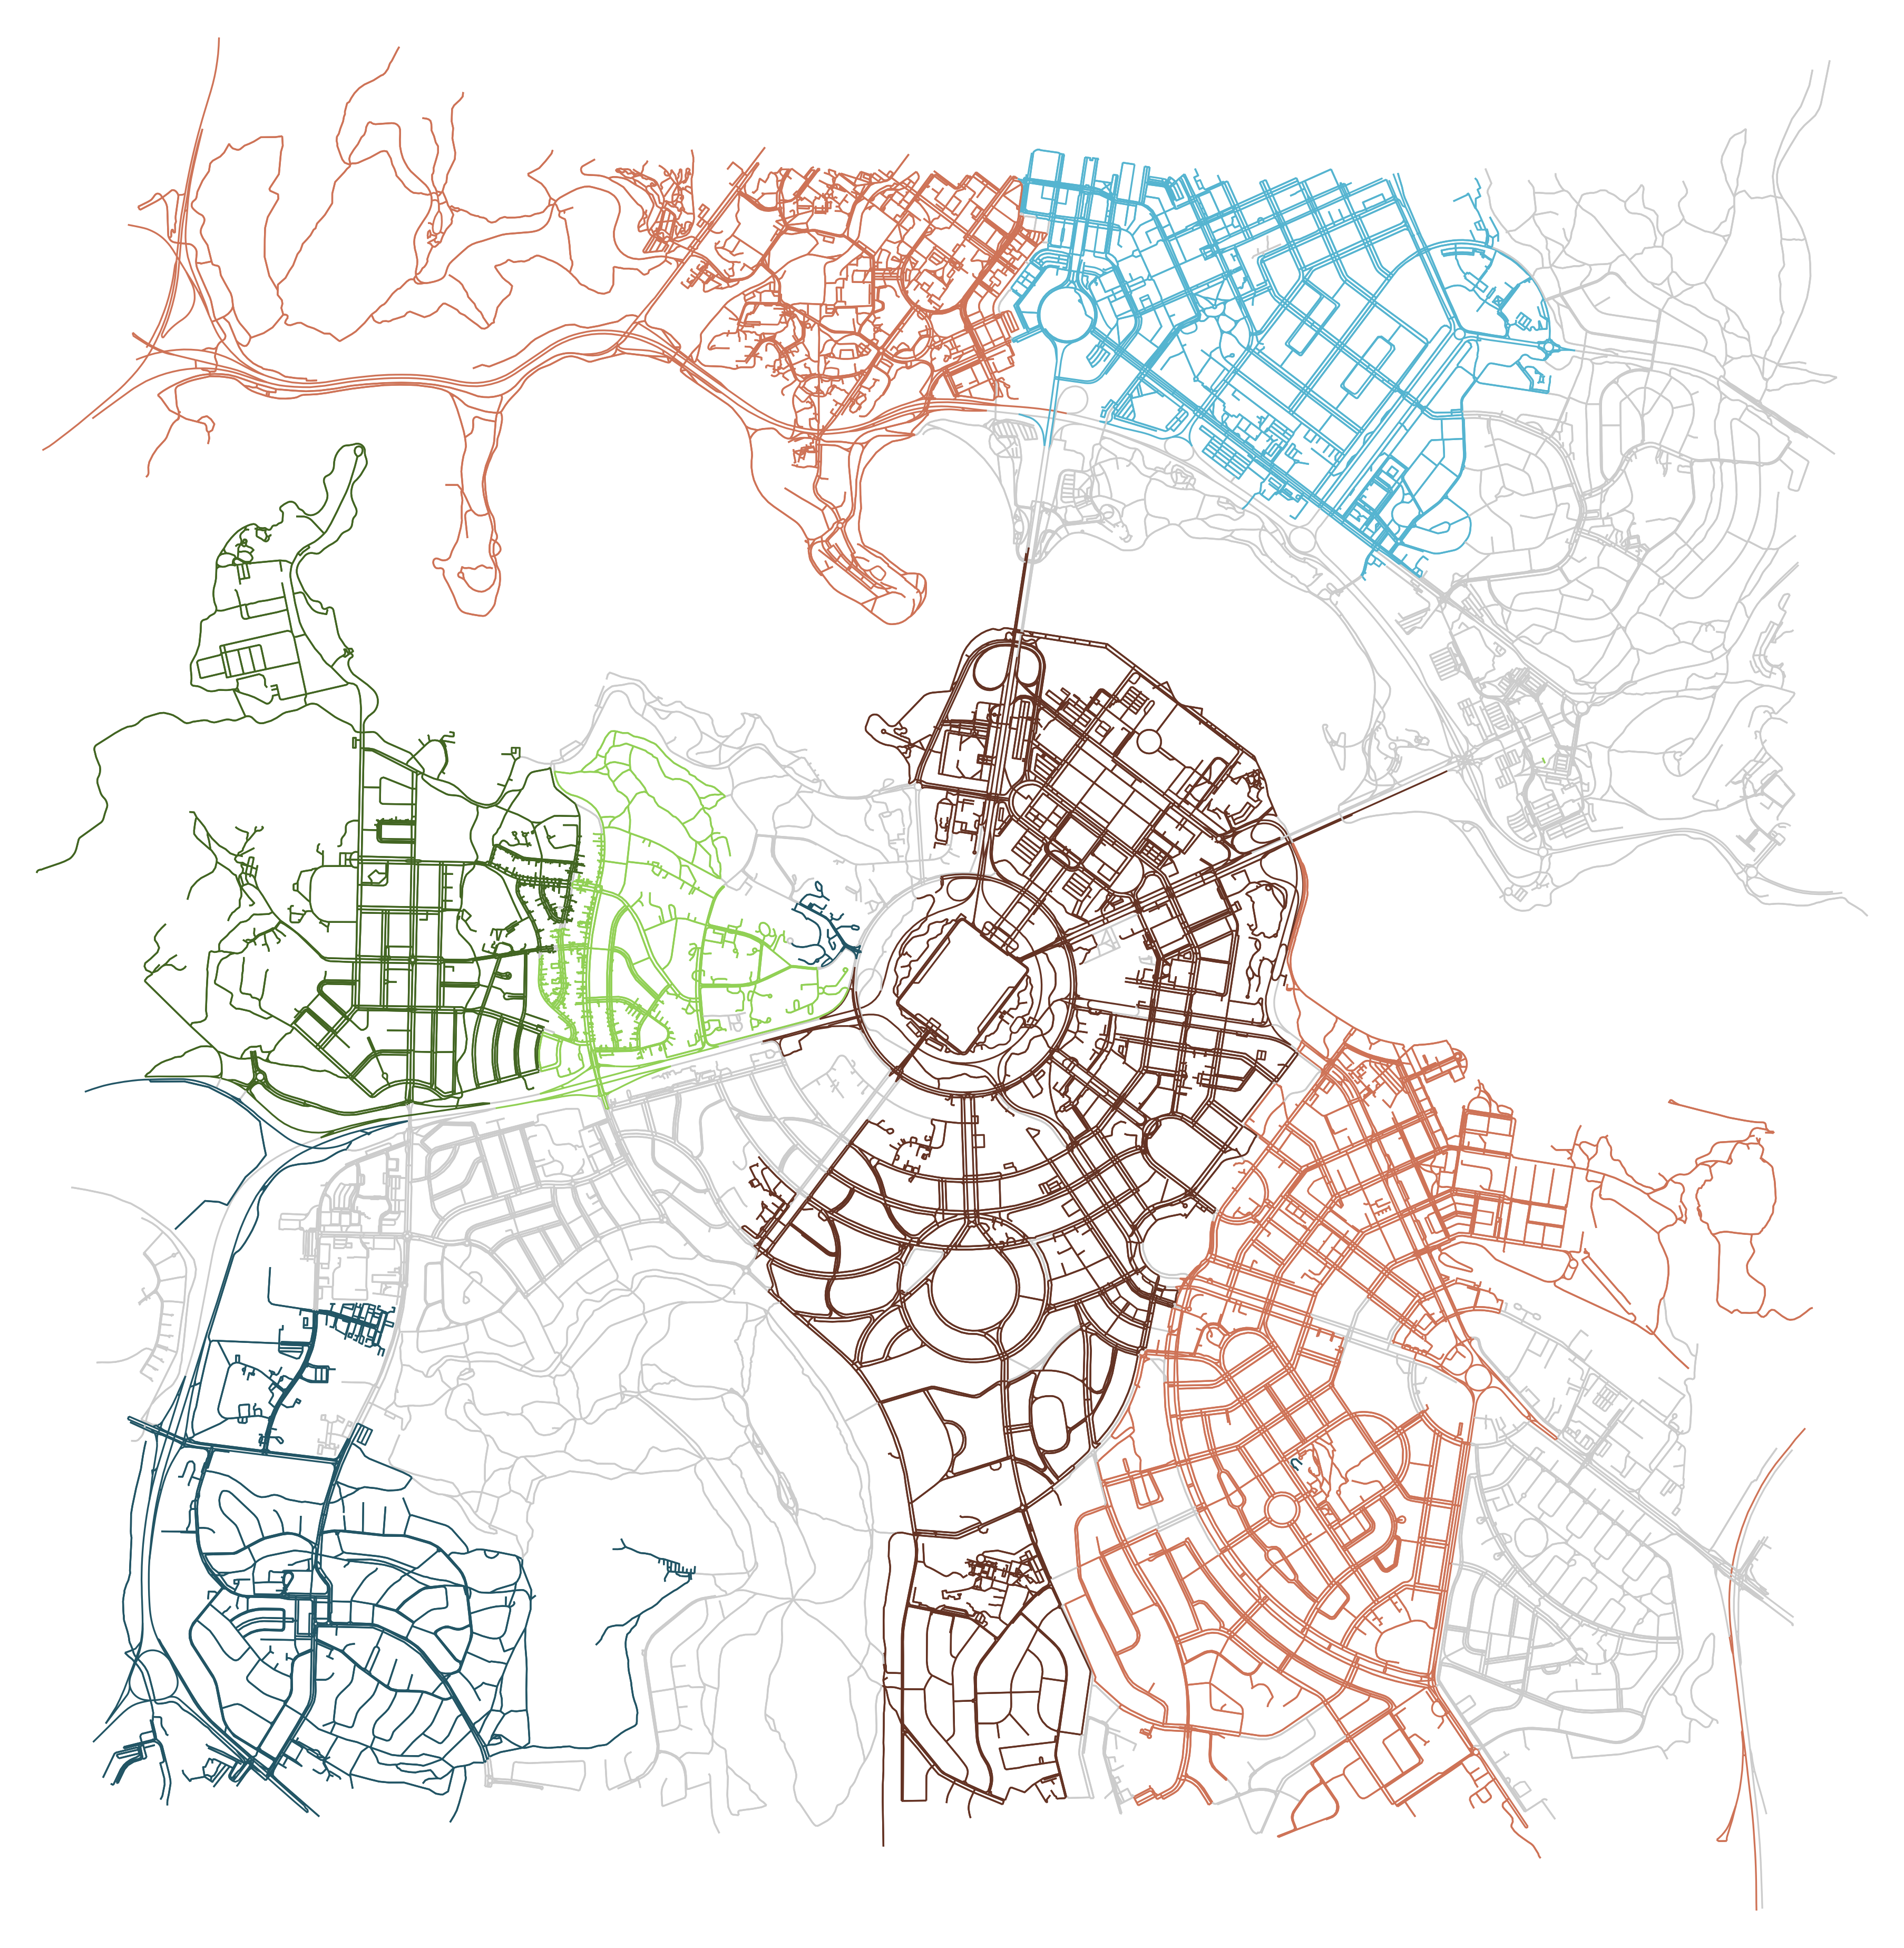
\includegraphics[width=0.85\linewidth]{maps/Canberra.png} \\[-0.5ex]
\bottomrule
\end{tabularx}
\end{adjustwidth}
\end{table}

\begin{table}[H]
\caption{Relational group of cities considered in this study: Los Angeles (USA), Berlin (Germany), Cairo (Egypt), and Amsterdam (Netherlands). For each city, the table provides basic data, the UMAP+HDBSCAN embedding, and the colored map projection at the chosen scale, together with the taxonomy label from Lima’s classification.}
\label{table_relational_embeddings}

\begin{adjustwidth}{-\extralength}{0cm}
%\centering %% If there is a figure in wide page, please release command \centering
\begin{tabularx}{\fulllength}{>{\raggedright\arraybackslash}X m{6cm}<{\centering}m{6cm}<{\centering}}
\toprule
\textbf{City Info} & \multicolumn{1}{c}{\textbf{Embedding}} & \multicolumn{1}{c}{\textbf{Map}} \\
\midrule
\textbf{{Los Angeles}} \newline Country: United States \newline Lat/Lon: (34.0293, $-$118.2144) \newline Scale: 1 km \newline Group: Relational \newline Taxonomy Label: \newline Flow Chart &
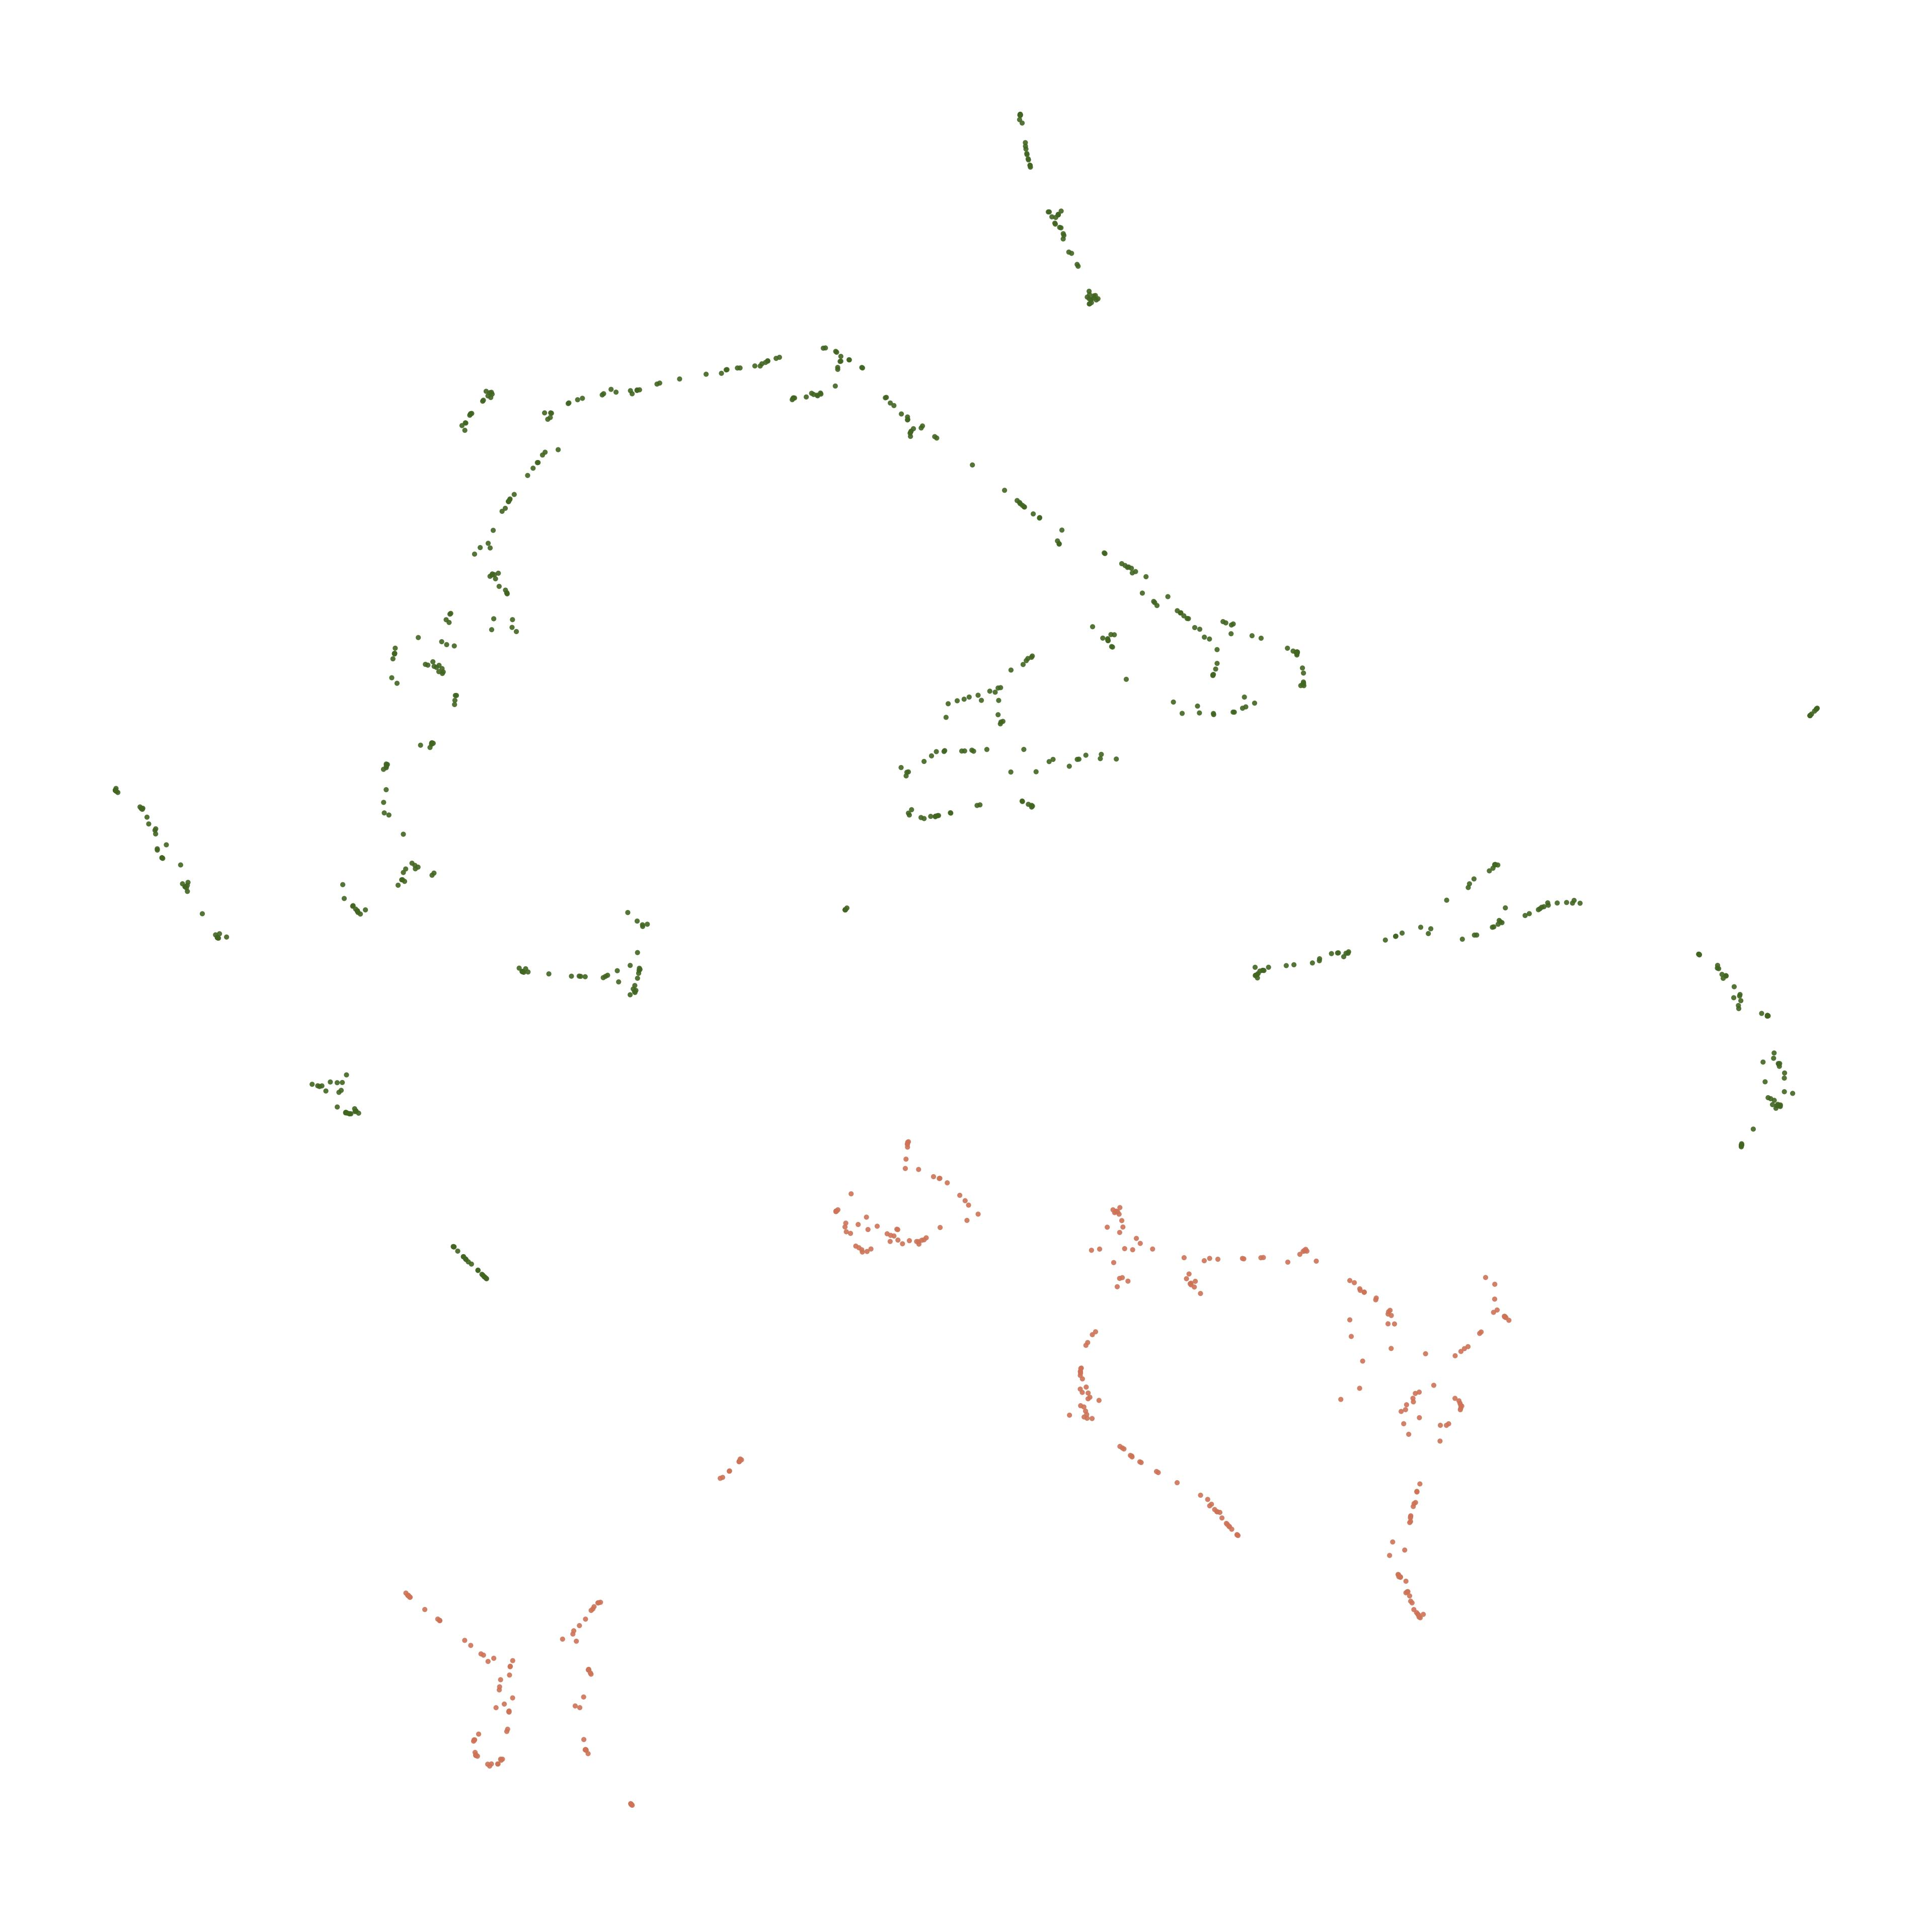
\includegraphics[width=0.9\linewidth]{clusters/Los_Angeles.jpg} &
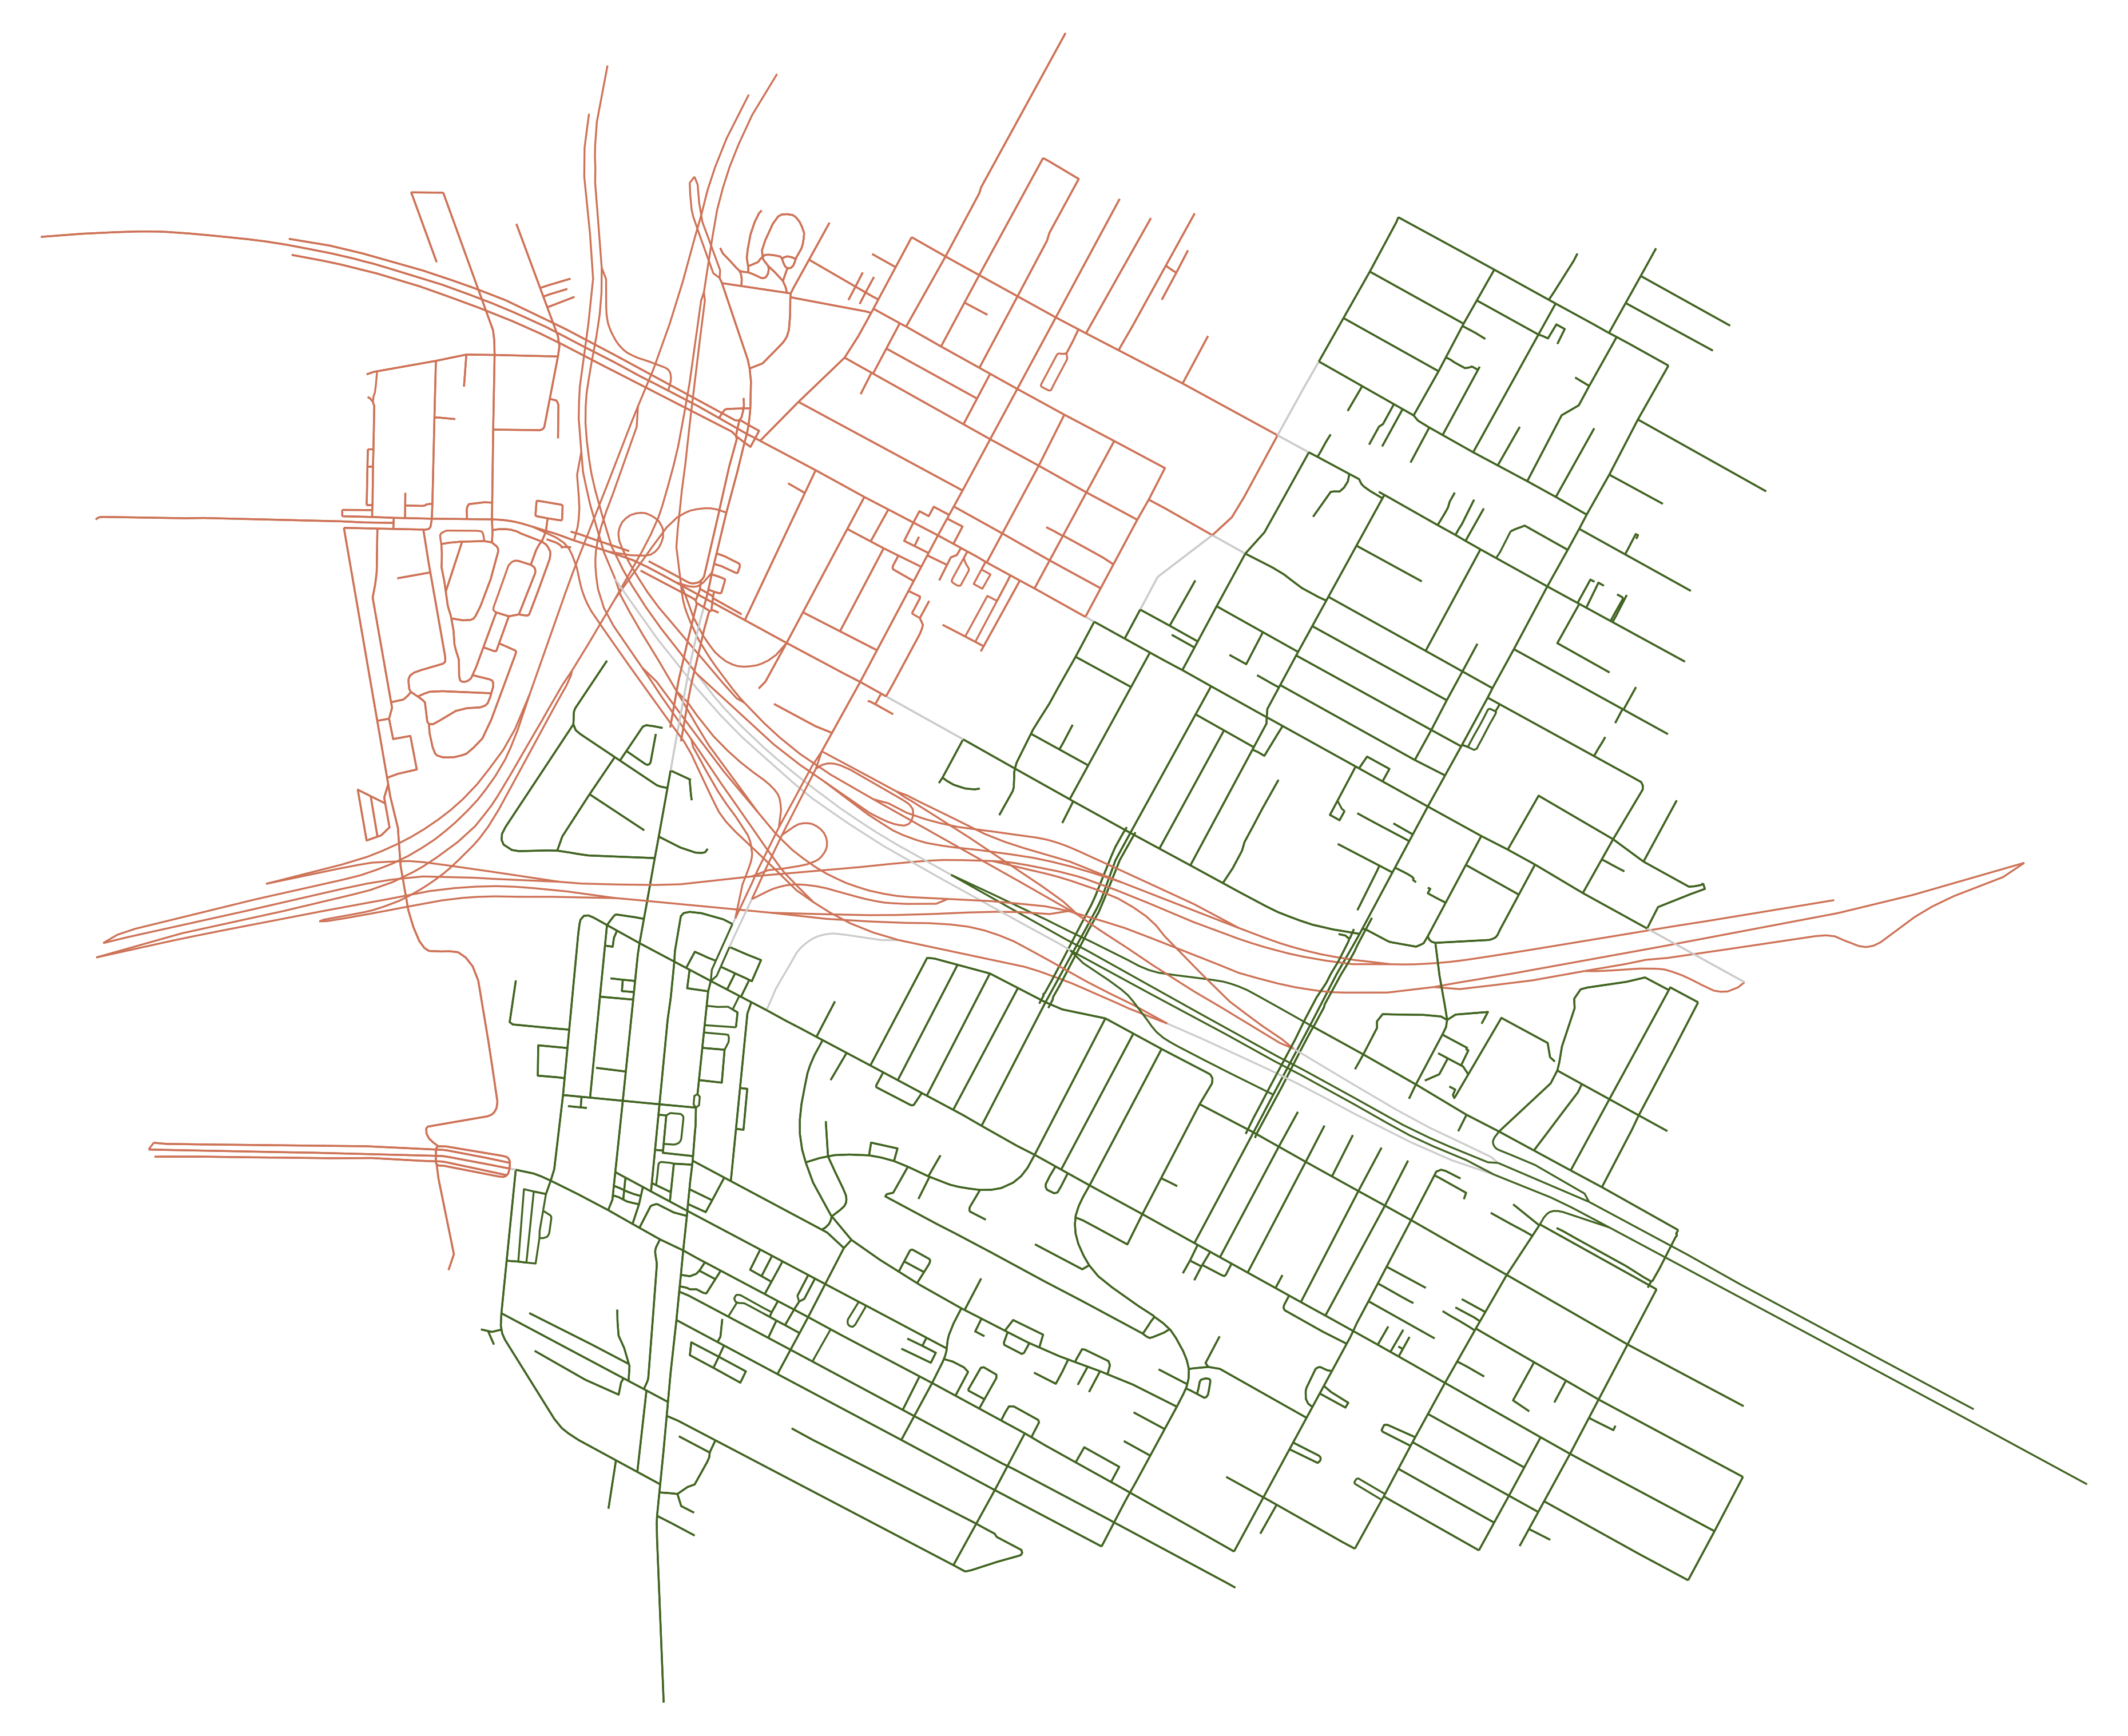
\includegraphics[width=0.9\linewidth]{maps/Los_Angeles.png} \\[-2.5ex]
\midrule
\textbf{{Berlin}} \newline Country: Germany \newline Lat/Lon: (52.5200, 13.4050) \newline Scale: 5 km \newline Group: Relational \newline Taxonomy Label: \newline Area Grouping &
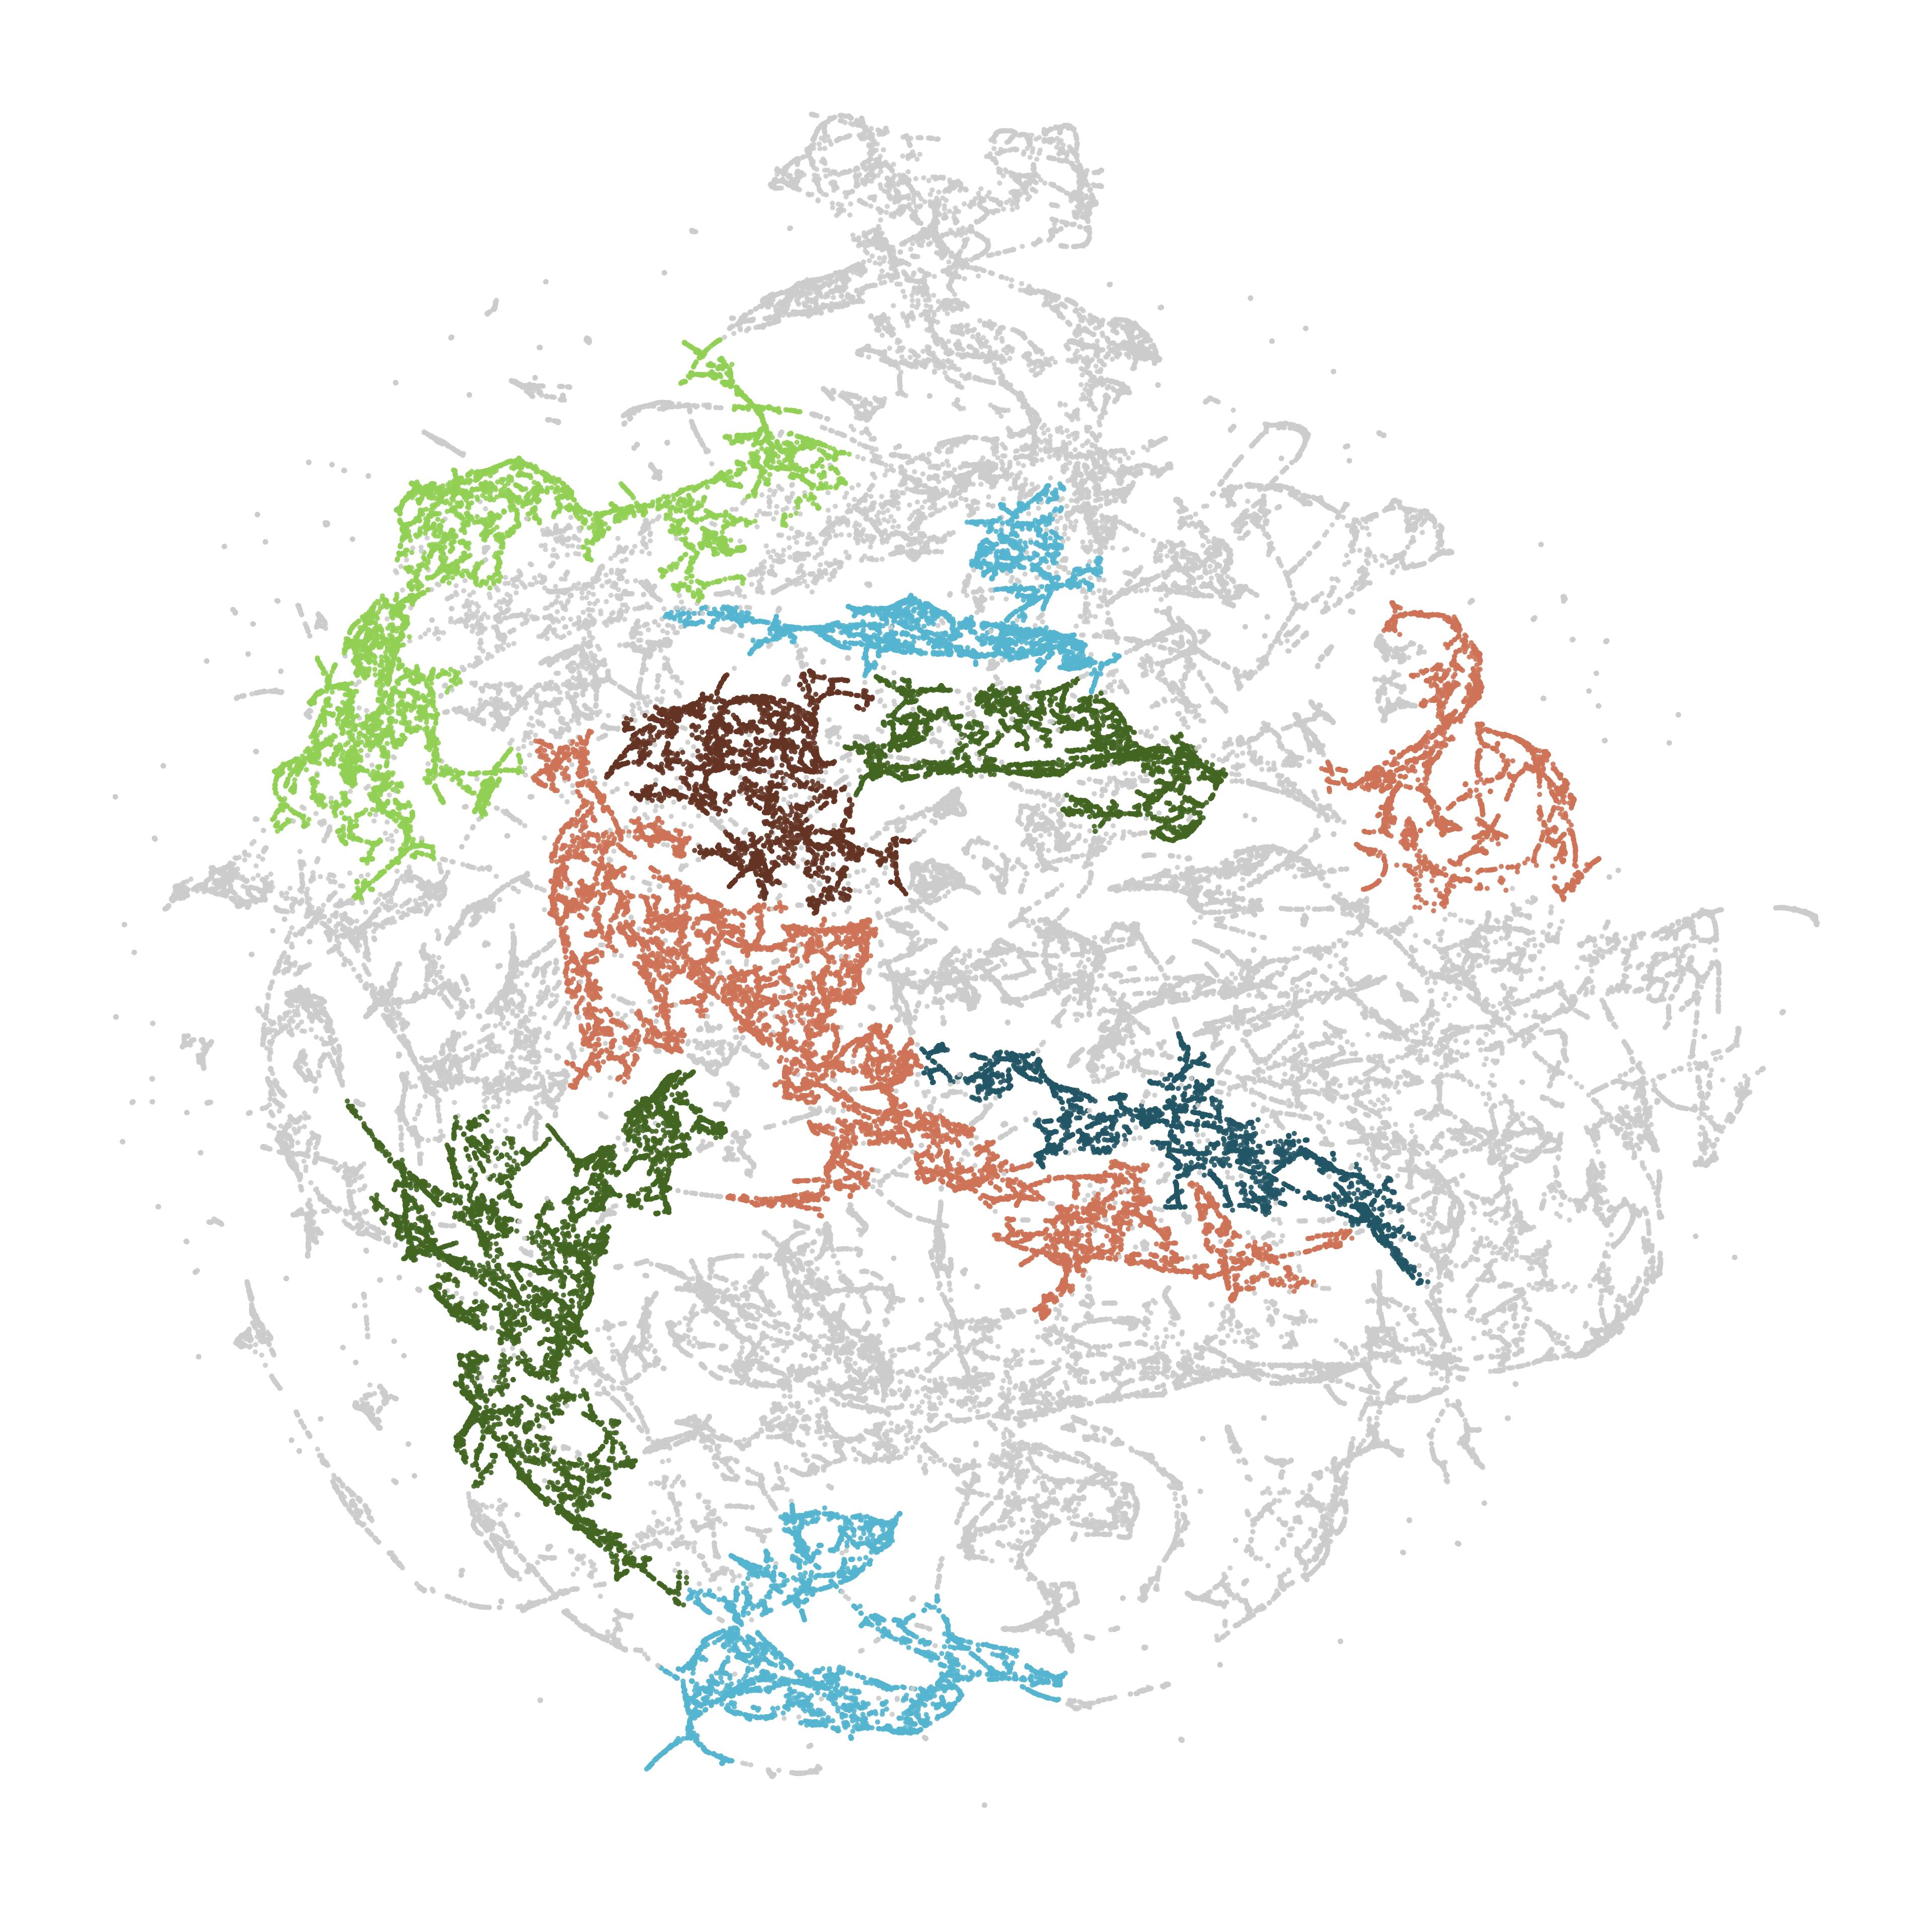
\includegraphics[width=0.9\linewidth]{clusters/Berlin.jpg} &
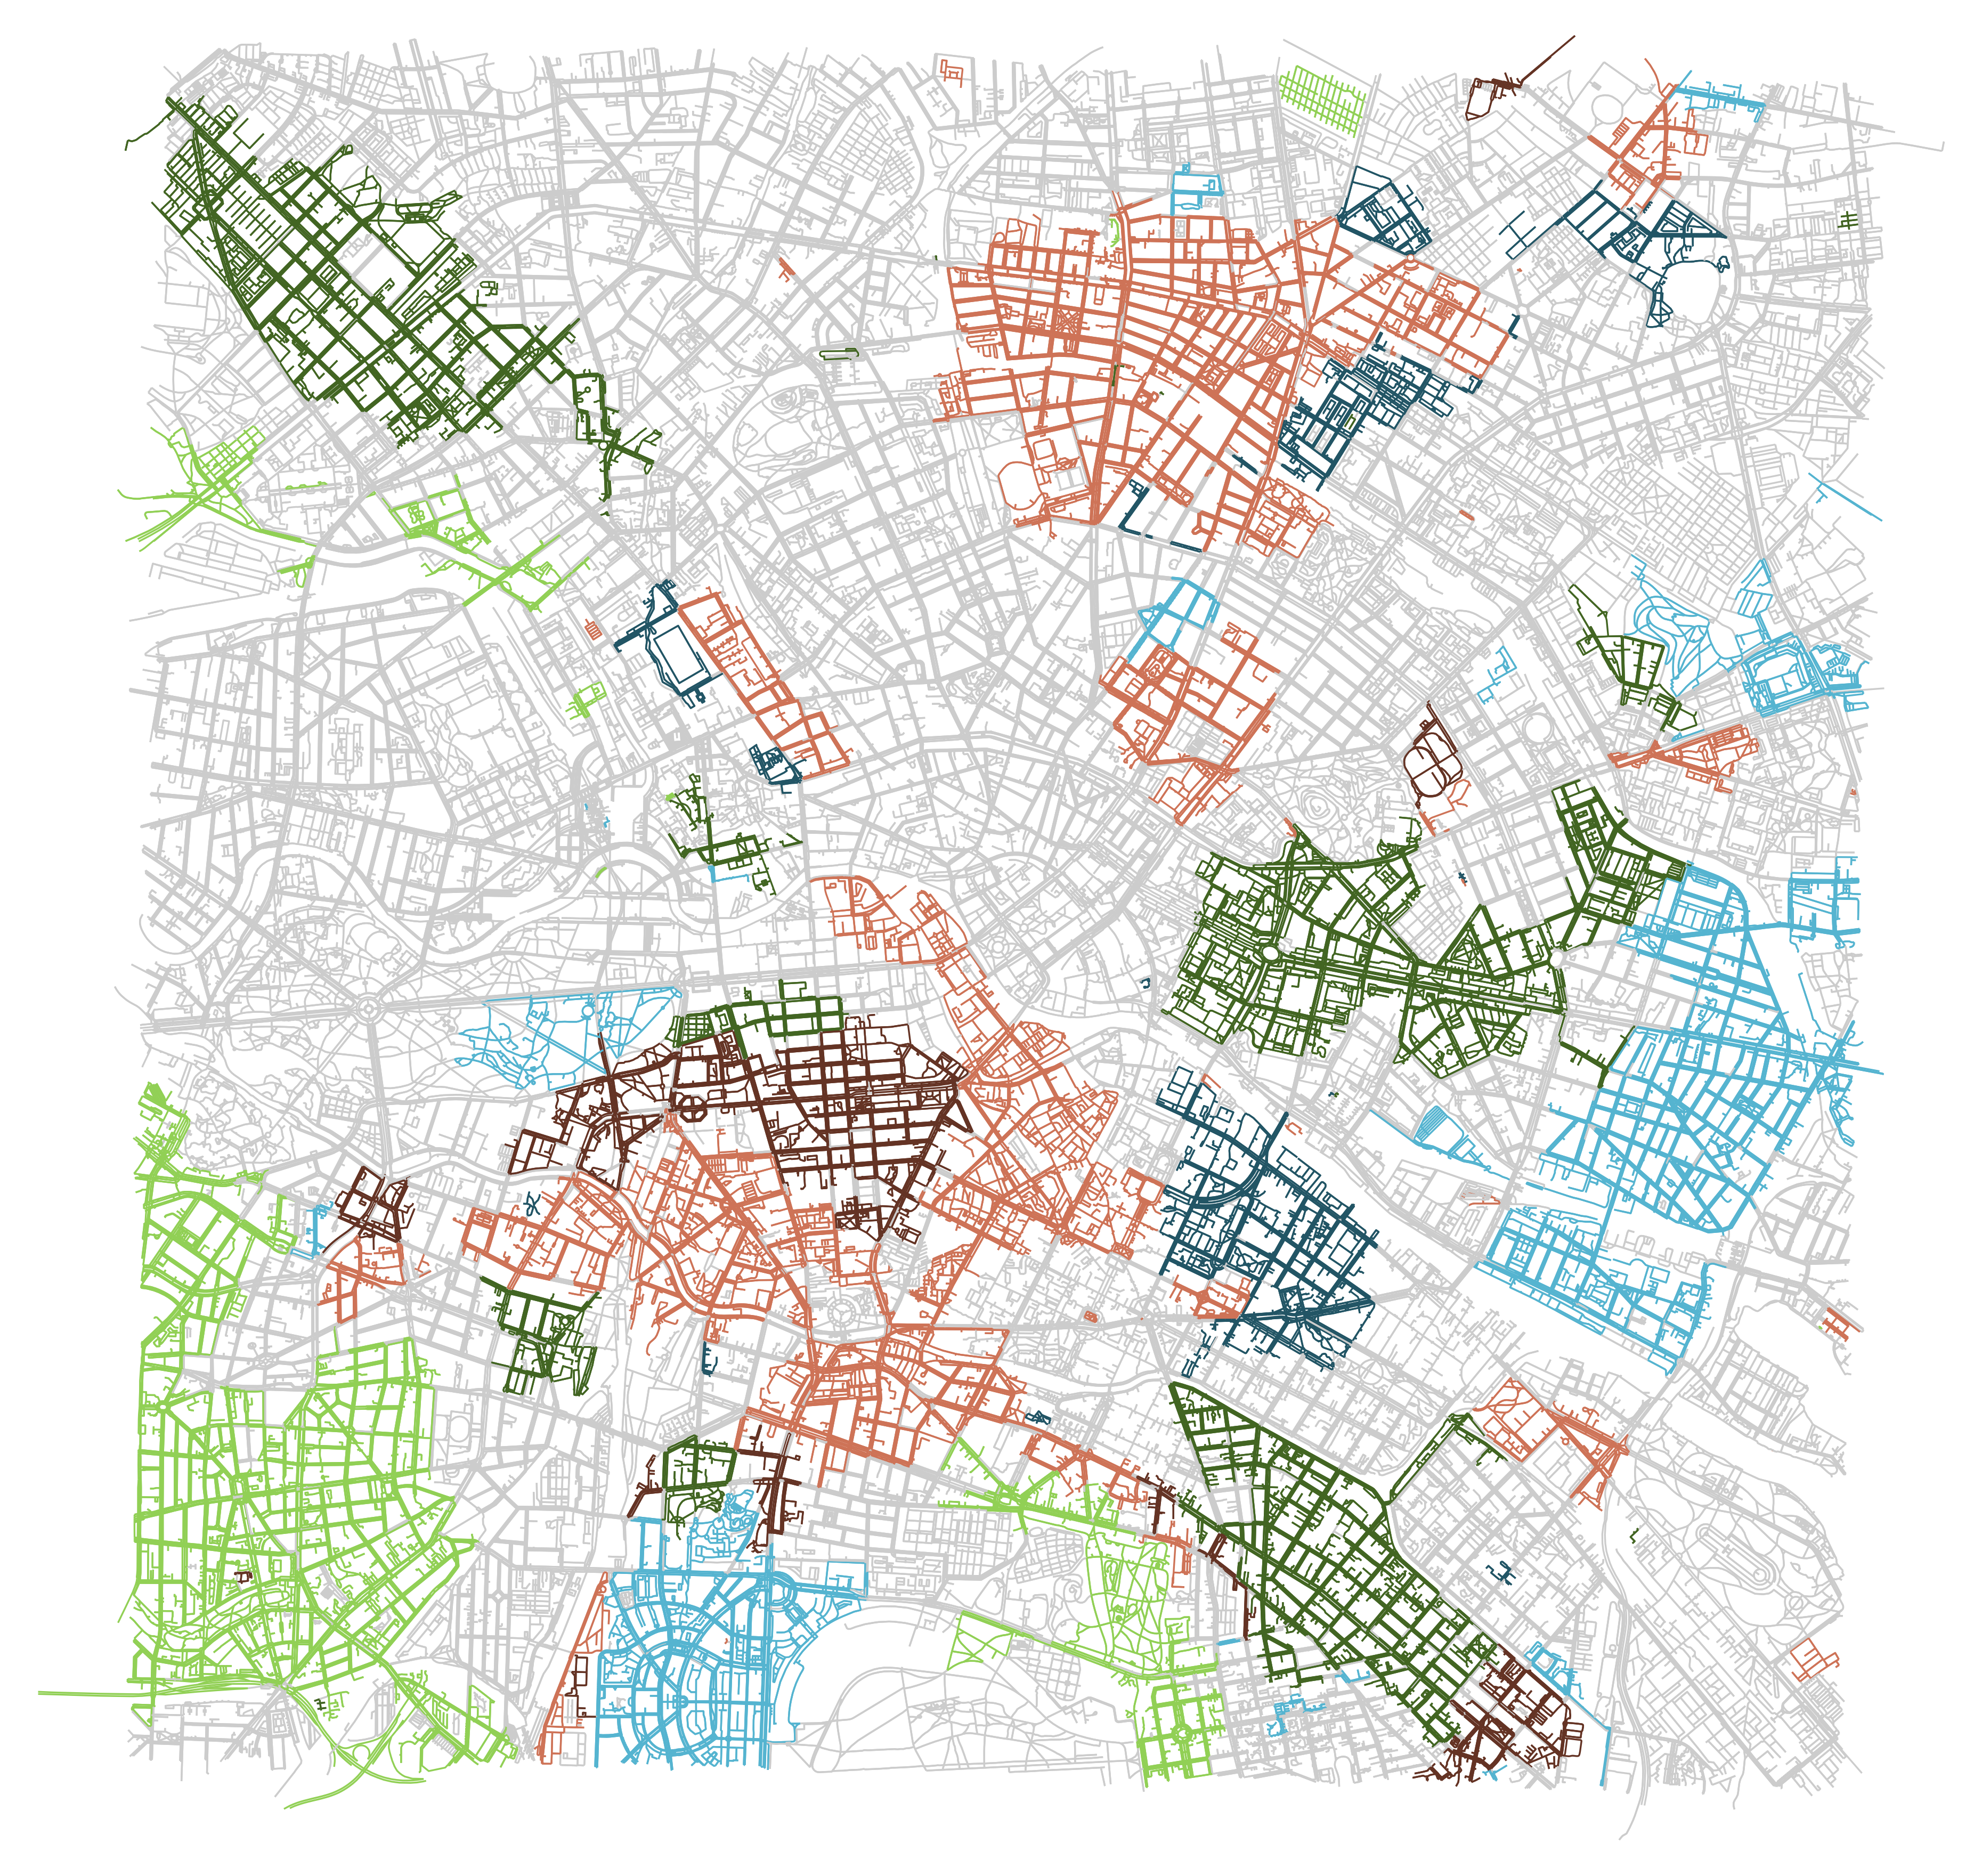
\includegraphics[width=0.9\linewidth]{maps/Berlin.png} \\[-2.5ex]
\midrule
\textbf{{Cairo}} \newline Country: Egypt \newline Lat/Lon: (30.0444, 31.2357) \newline Scale: 5 km \newline Group: Relational \newline Taxonomy Label: \newline Circular Ties &
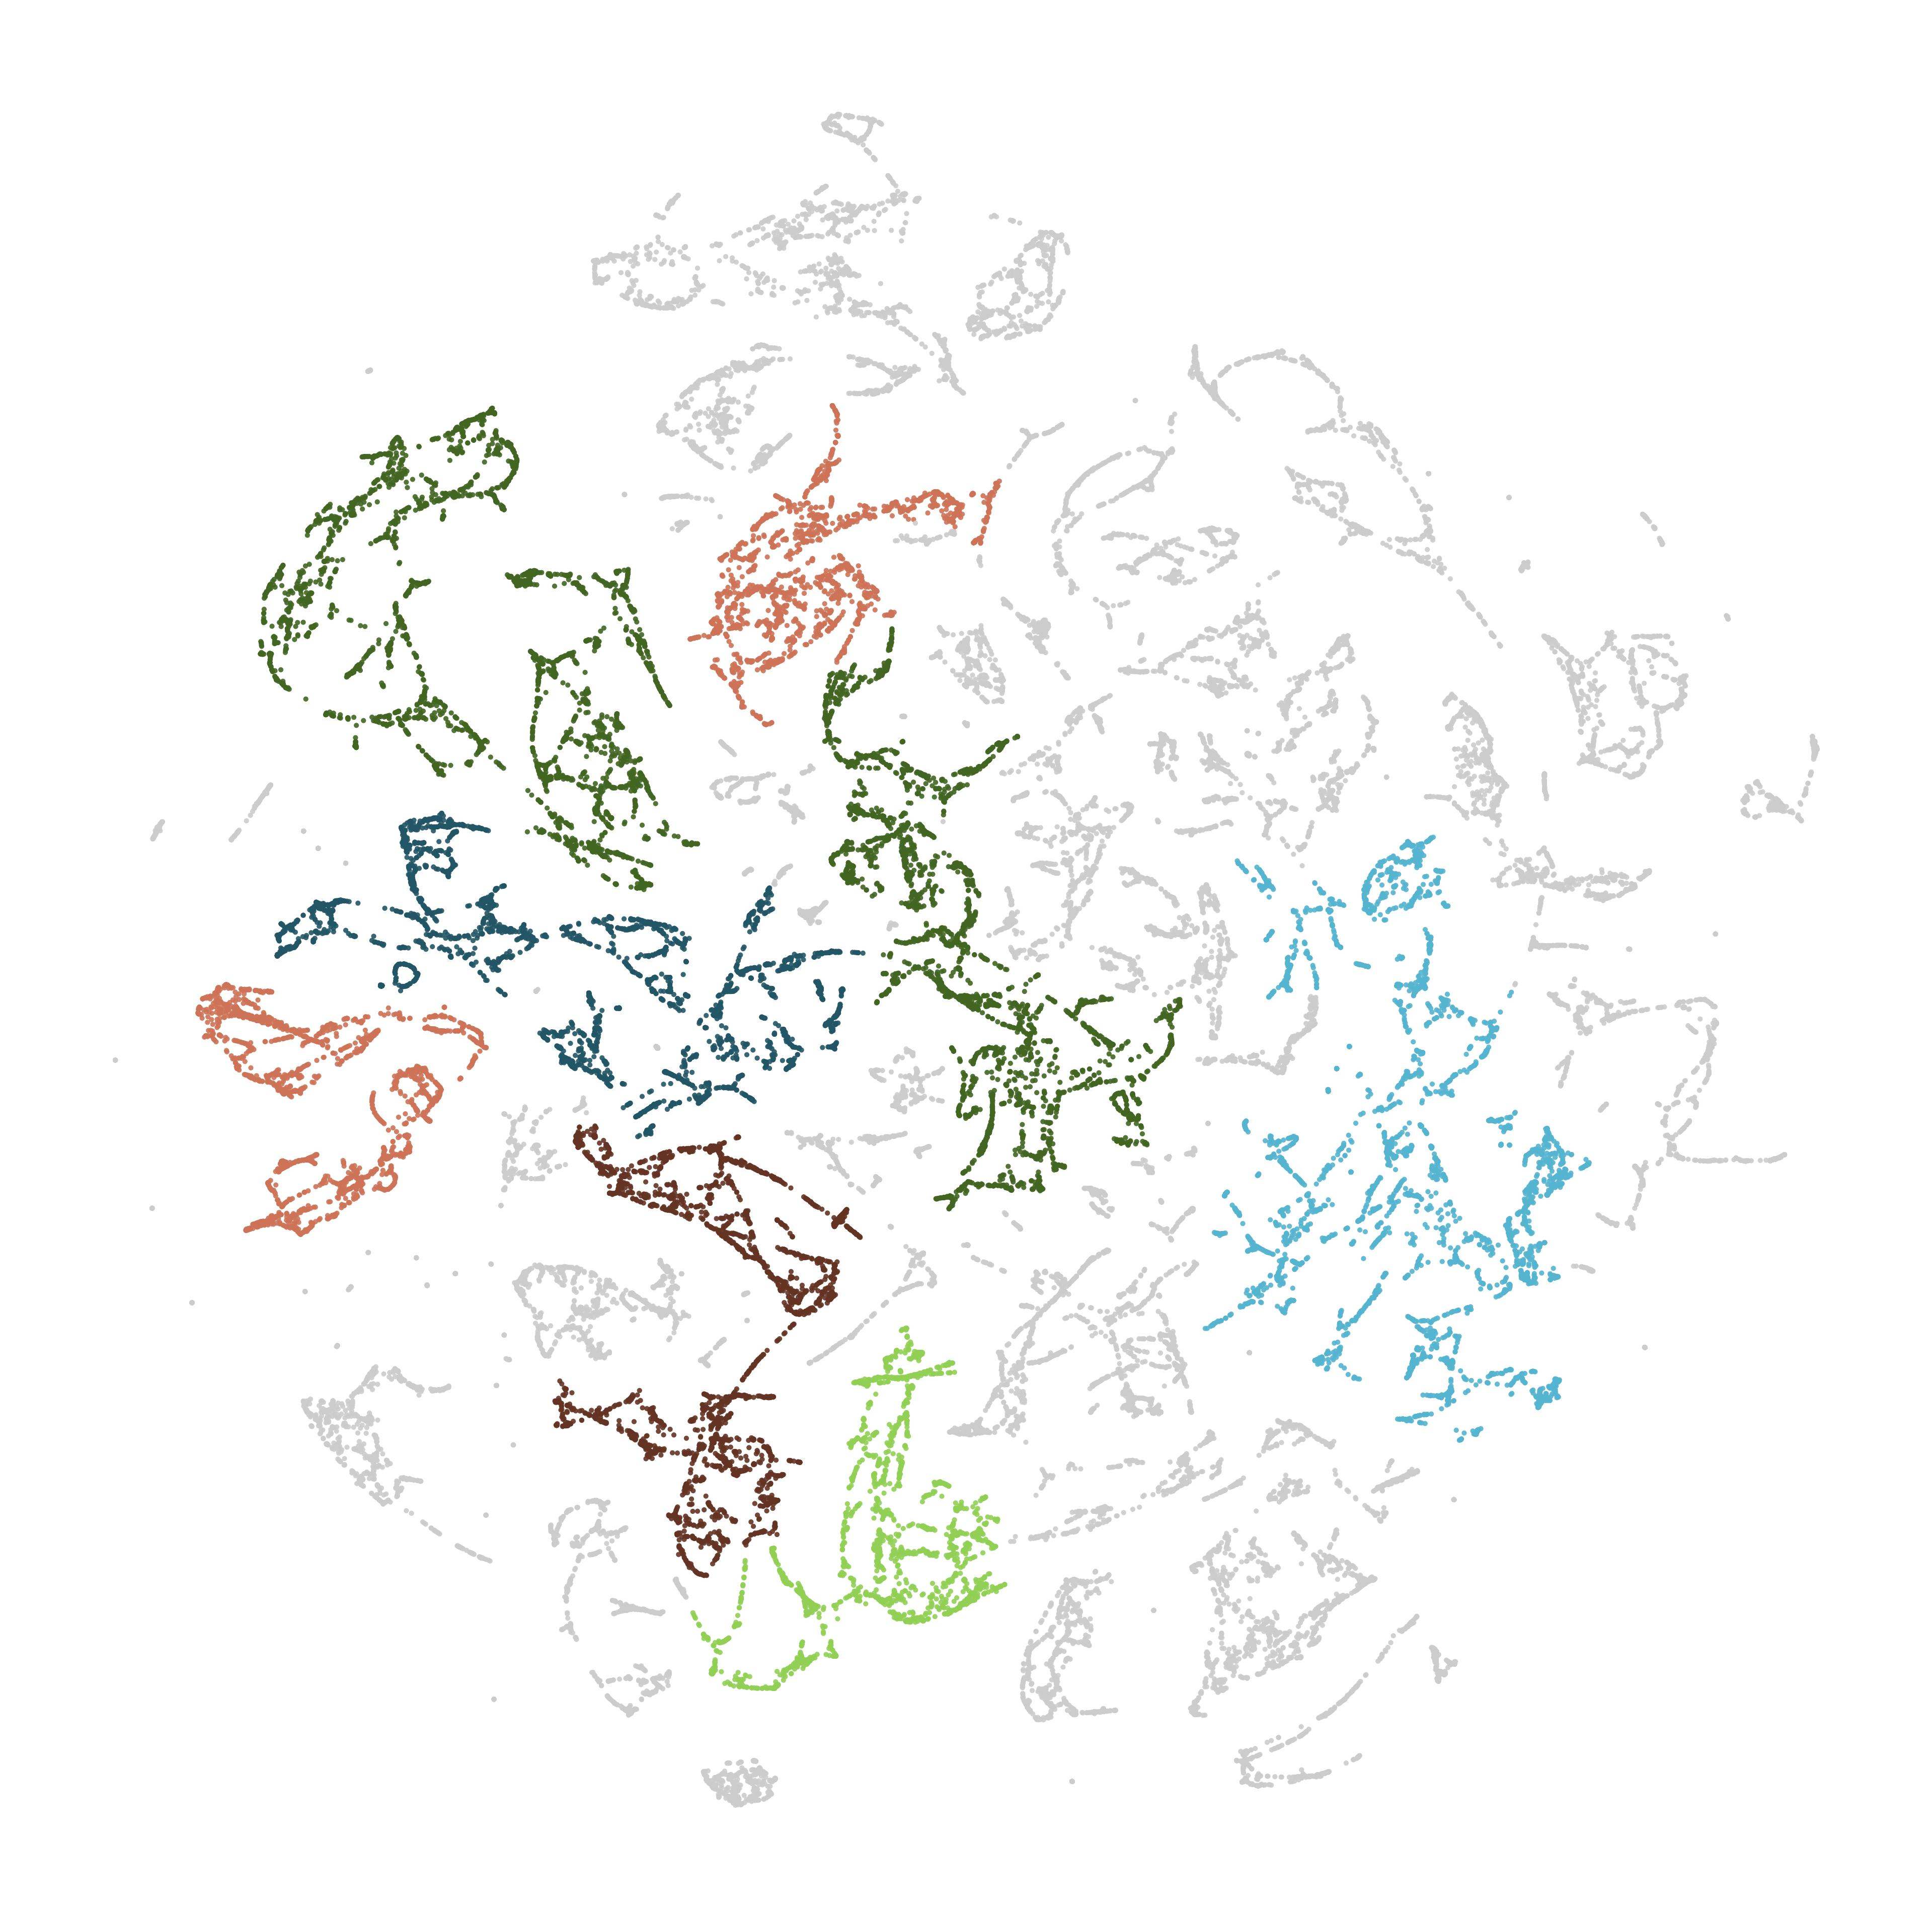
\includegraphics[width=0.9\linewidth]{clusters/Cairo.jpg} &
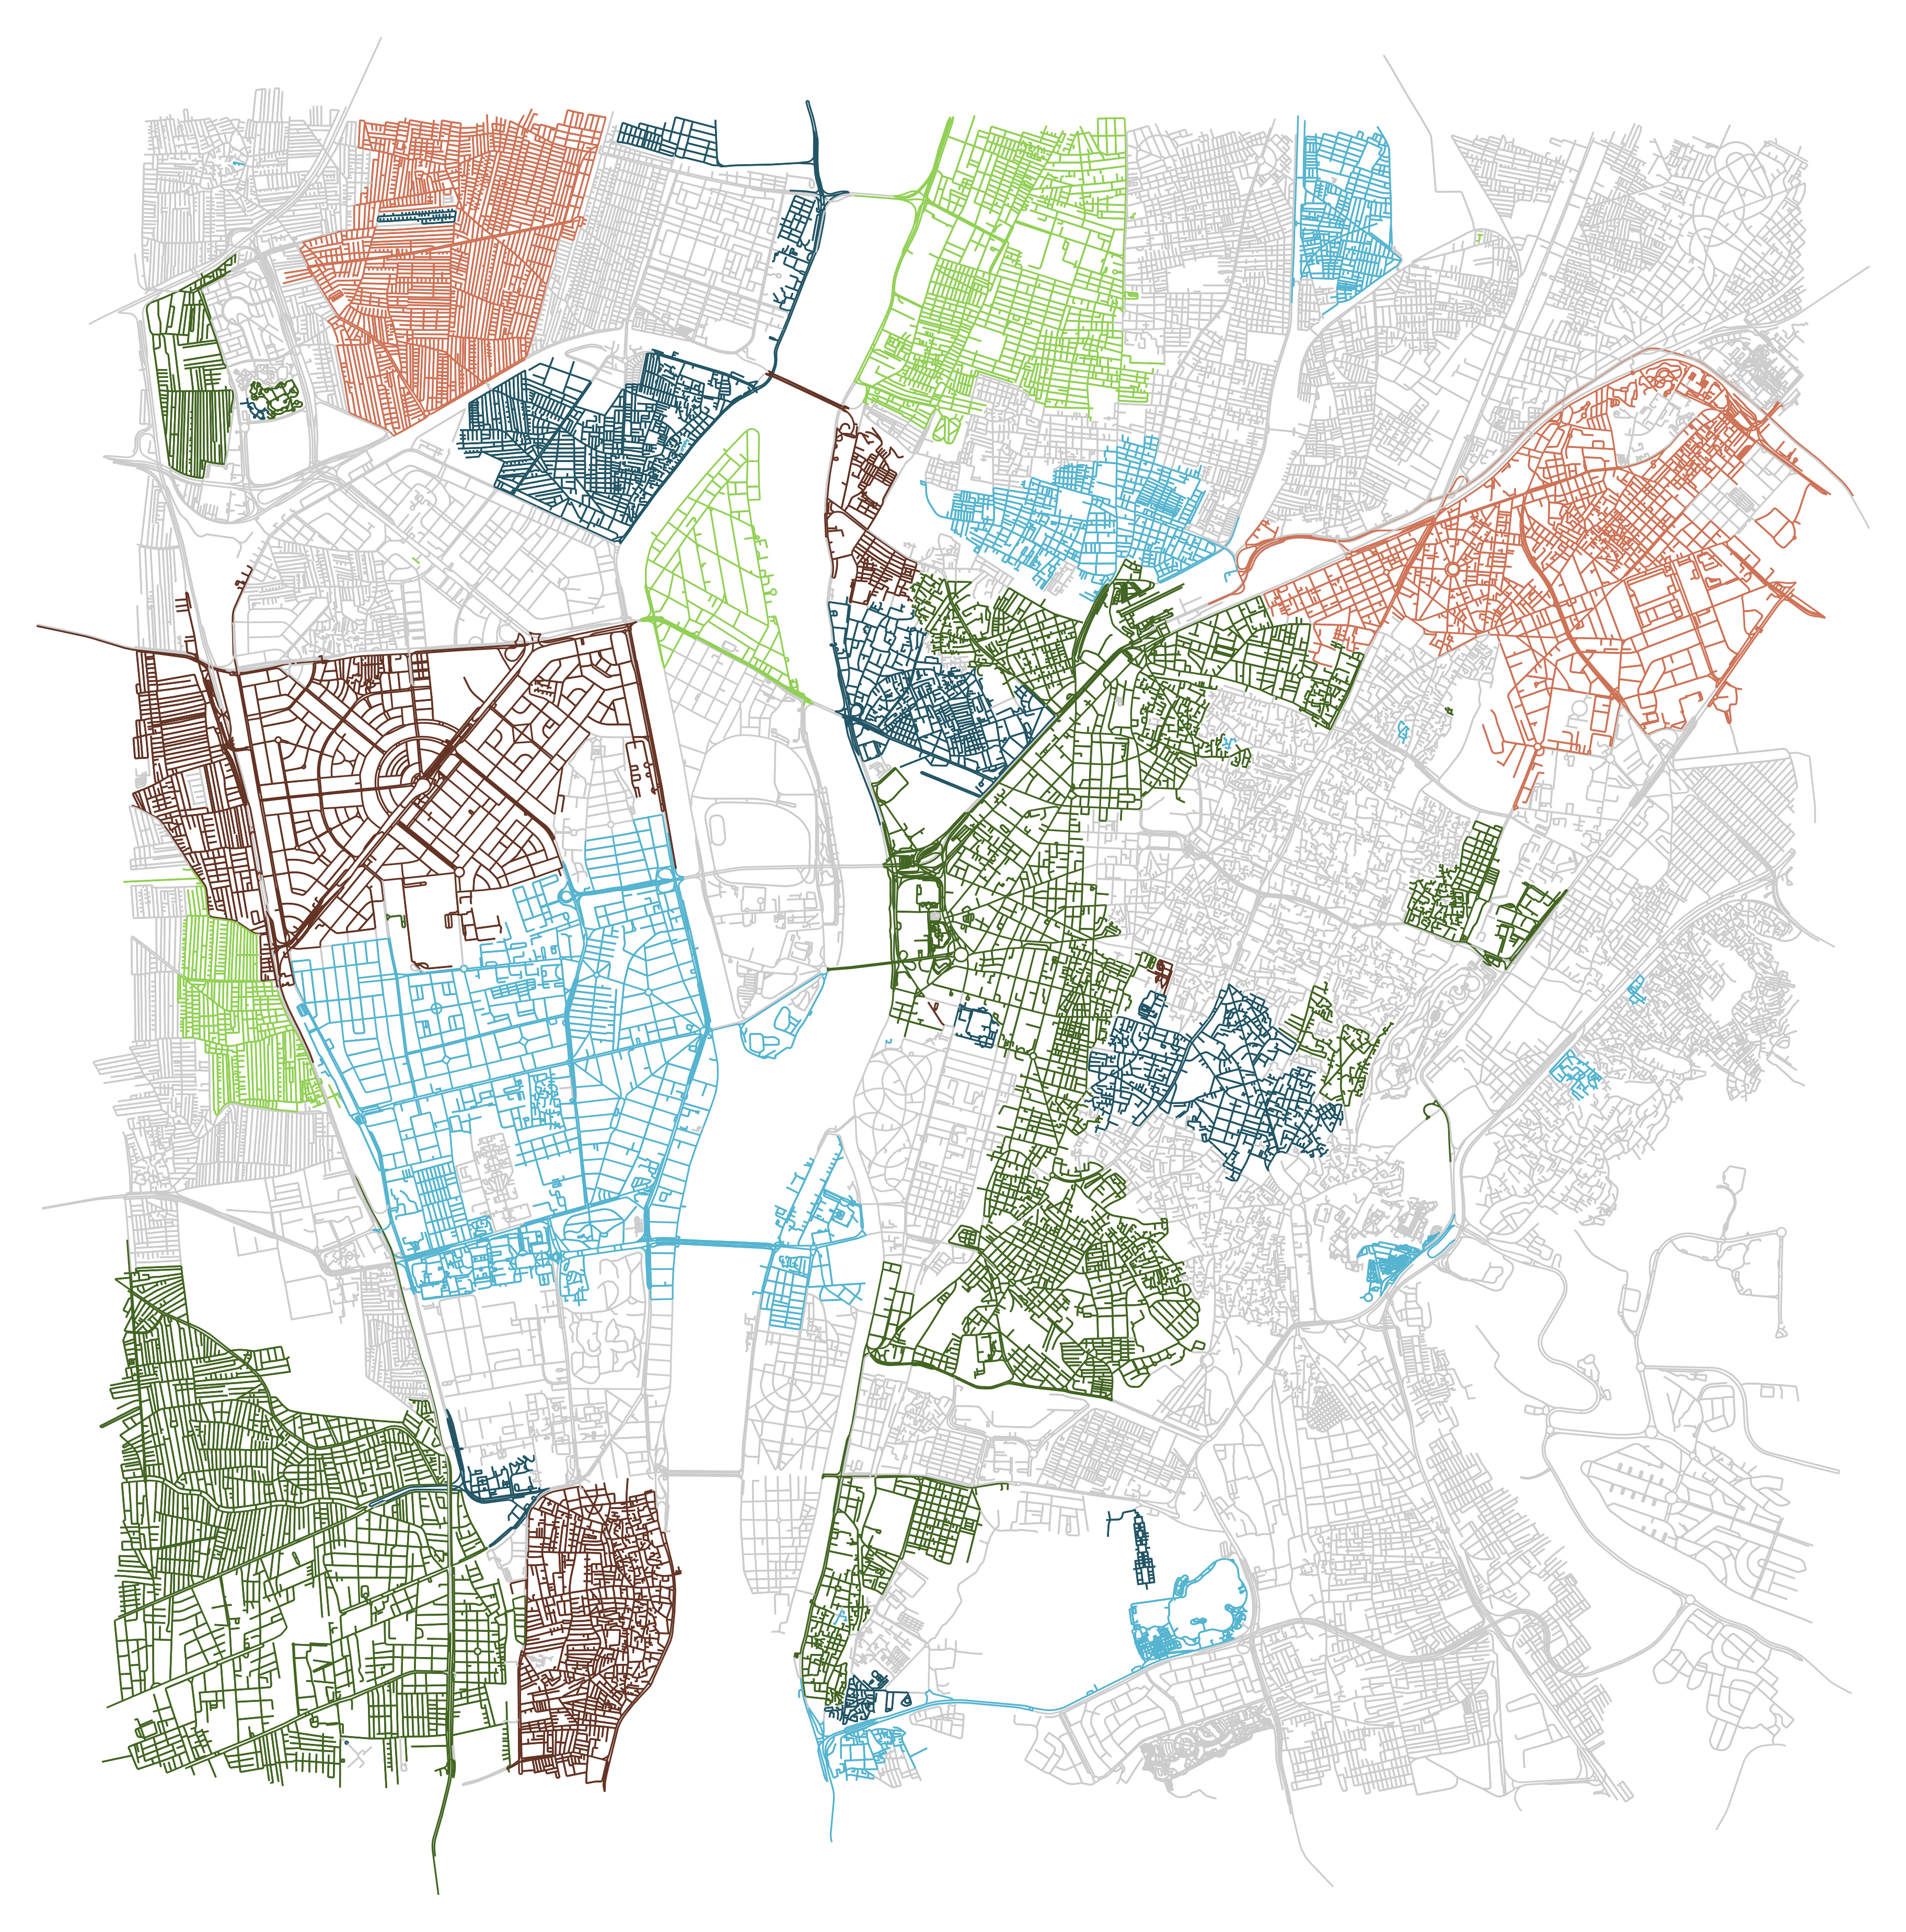
\includegraphics[width=0.9\linewidth]{maps/Cairo.png} \\[-0.5ex]
\midrule
\textbf{{Amsterdam}} \newline Country: Netherlands \newline Lat/Lon: (52.3710, 4.9000) \newline Scale: 2 km \newline Group: Relational \newline Taxonomy Label: \newline Ramification &
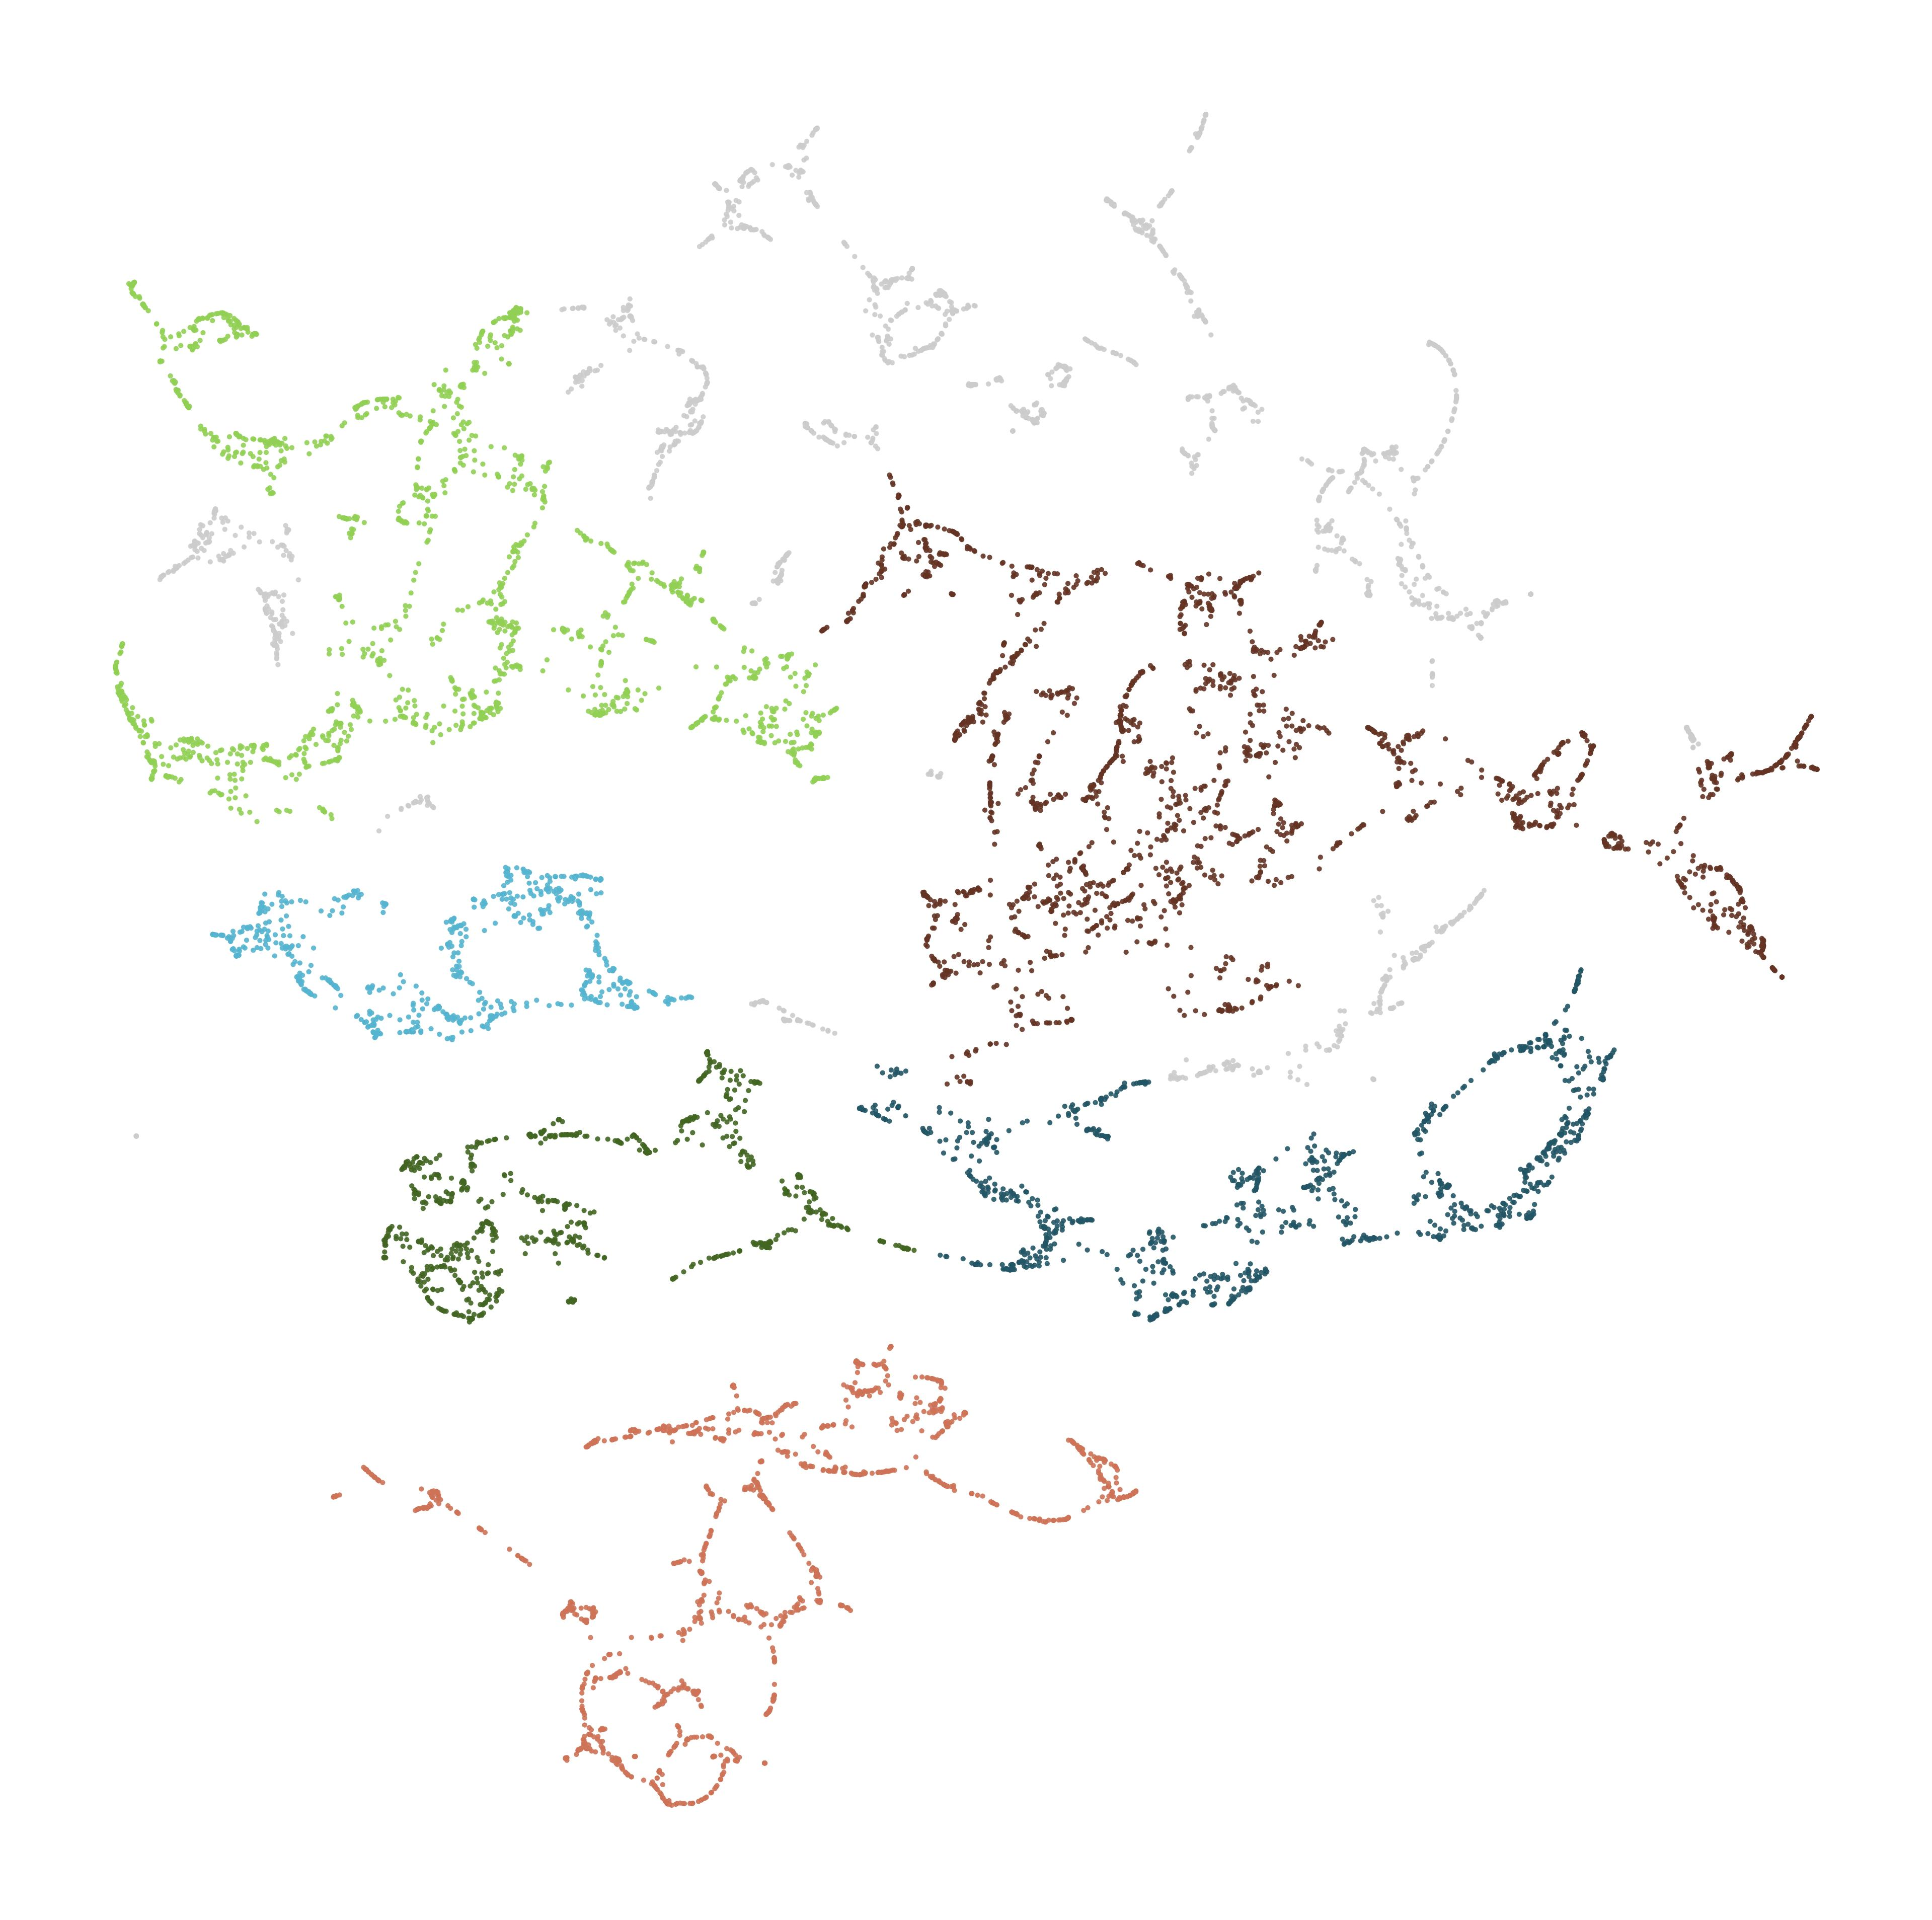
\includegraphics[width=0.9\linewidth]{clusters/Amsterdam.jpg} &
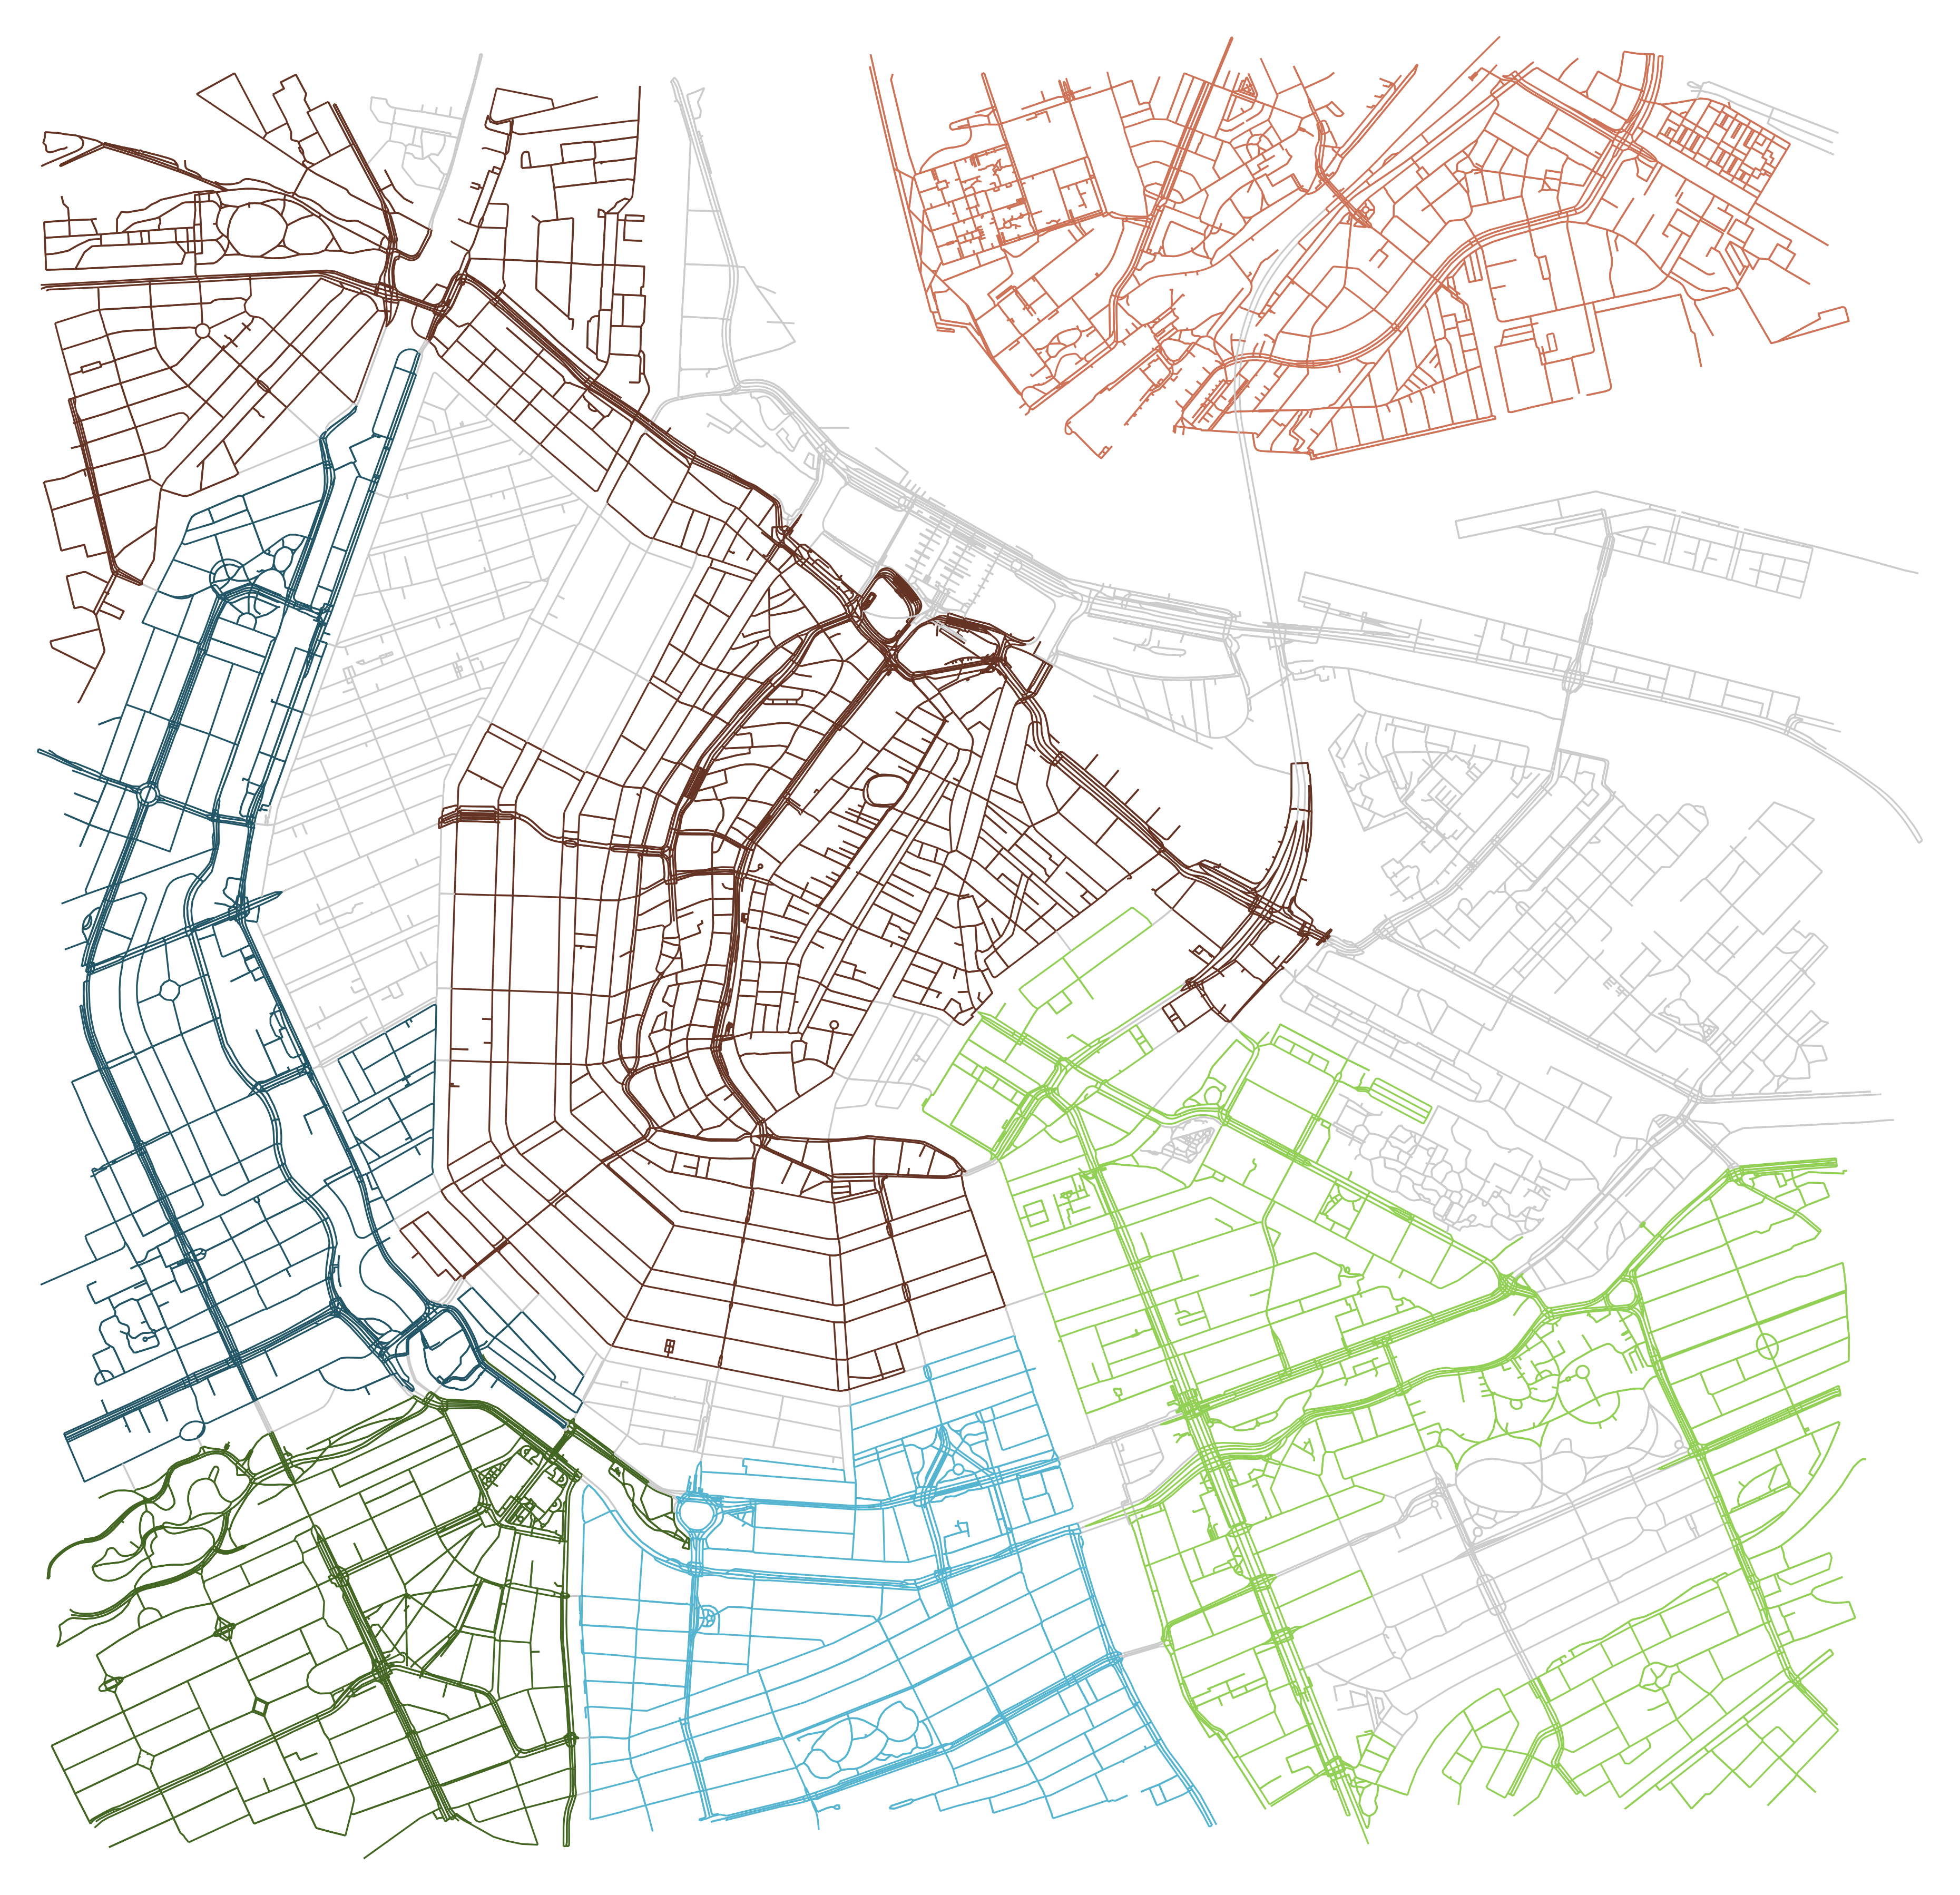
\includegraphics[width=0.9\linewidth]{maps/Amsterdam.png} \\[-0.5ex]
\bottomrule
\end{tabularx}
\end{adjustwidth}
\end{table}

%%%%%%%%%%%%%%%%%%%%%%%%%%%%%%%%%%%%%%%%%%%%%%%%%%%%%%%%%%%%%%%%%%%%%%%
%                                                                     %
%                          Section 5                                  %
%                          Discussion                                 %
%                                                                     %
%%%%%%%%%%%%%%%%%%%%%%%%%%%%%%%%%%%%%%%%%%%%%%%%%%%%%%%%%%%%%%%%%%%%%%%

\section{Discussion}\label{sec5}
The findings underline that scale is a decisive parameter for network-based urban analysis. Compact morphologies generate embeddings that remain legible and coherent, while sprawling metropolitan fabrics tend to dissolve into incoherence. This points not only to the strengths but also to the fragility of the method, which must be carefully calibrated to the scale of inquiry. Equally important is the recognition that computational workflows are not neutral: every stage---from data extraction to clustering---embeds assumptions about what counts as a street or neighborhood. To mitigate these blind spots, the workflow has been made transparent and reproducible through the GitHub repository \cite{rodighiero_urban-mapper_2025}, where the steps and scripts can be inspected, reused, and adapted by others.

At present, the methodology relies on a limited dataset consisting of street networks derived from {OSMnx}. This provides a useful baseline but does not capture the full range of urban dynamics. Graphs could be enriched with weights expressing flows of pedestrians, bicycles, cars, and public transport, giving greater significance to heavily used connections. Similarly, networks could integrate additional infrastructures and demographic \mbox{layers---such} as population density, land use, or service distribution---to refine precision. The framework should therefore be understood as an open structure, capable of accommodating more complex data, rather than a closed or definitive system. Its modularity is intentional: the workflow is meant to serve as a foundation that can be extended with further layers of spatial or social information, depending on the research questions at hand.

Beyond technical adjustments, the discussion must also consider broader implications. Visualization is never a neutral window but an interpretative practice, and design choices carry rhetorical and political weight, as Johanna Drucker reminds us \cite{drucker_graphesis_2014}. Decisions about which data to include or exclude have ethical consequences, shaping which actors and infrastructures are made visible or hidden. These concerns also point toward future directions: while the present study is cross-sectional, the same workflow could be extended longitudinally, tracing transformations in morphology over time and offering insight into how networks evolve. Such temporal extensions would enable observation of how urban fabrics adapt across decades, allowing designers and historians alike to explore change not only spatially but dynamically.

The contribution of this study lies in advancing what can be called \textit{{network literacy}} for urban design. Network methods do not replace traditional cartography; rather, they complement it, providing a dual lens through which urban form can be understood both territorially and relationally. This dual vision supports adaptive and interdisciplinary practice, bridging design, data science, and urban studies. In this respect, the article extends earlier reflections on network literacy in design \cite{rodighiero_network_nodate}, demonstrating how its principles can be applied to questions of morphology and infrastructure in the contemporary city. Understood in this way, network literacy equips practitioners with a grammar for interpreting not only what cities are but also how they operate as systems of relations.

From a practical perspective, this dual lens is most useful as a complementary method in contexts where understanding connectivity is crucial. The workflow proves especially effective in compact and medium-scale urban fabrics, where embeddings remain legible, and in neighborhoods undergoing transformation, where topological analysis can complement cartographic views to identify shifting alignments. It can also be valuable in planned environments, where the resilience of geometric order can be tested, and in evolving metropolitan areas, where dispersion, peripherality, or infrastructural isolation becomes visible. In addition, its prospective use as a form of simulation allows planners to anticipate how proposed modifications might reshape the relational fabric of a city. Rather than replacing existing approaches, it extends the interpretive and diagnostic repertoire available to urban design.

%%%%%%%%%%%%%%%%%%%%%%%%%%%%%%%%%%%%%%%%%%%%%%%%%%%%%%%%%%%%%%%%%%%%%%%
%                                                                     %
%                          Section 6                                  %
%                         Conclusions                                 %
%                                                                     %
%%%%%%%%%%%%%%%%%%%%%%%%%%%%%%%%%%%%%%%%%%%%%%%%%%%%%%%%%%%%%%%%%%%%%%%

\section{Conclusions}\label{sec6}

Yaneva and Latour called for tools akin to a photographic gun, able to register the city’s movements rather than freeze it in static form. The workflow proposed here takes a step in that direction by reframing urban morphology through network visualizations that reveal continuities, disruptions, and fragile alignments. While the approach remains limited---its effectiveness varying by scale and by the scope of data included---it demonstrates how embeddings can extend cartography by tracing relations that maps alone cannot capture.

The contribution is both theoretical and practical. By situating network visualization within design theory, this study shows how urban form can be read simultaneously as enduring and relational. By making the workflow transparent and reproducible, it offers a structure that others can adapt, enrich, and extend with additional data. Above all, the conclusions reinforce the need for sustained interdisciplinary collaboration: network literacy provides designers, planners, data scientists, and urban researchers with a shared grammar for engaging the city as a dynamic, negotiated, and ever-changing assemblage.


\vspace{6pt}


\funding{{This research received no external funding.}%MDPI: Please add: ``This research received no external funding'' or ``This research was funded by NAME OF FUNDER grant number XXX.'' and  and ``The APC was funded by XXX''. Check carefully that the details given are accurate and use the standard spelling of funding agency names at \url{https://search.crossref.org/funding}, any errors may affect your future funding.
}

\dataavailability{{The} %MDPI: We modified it according to the rules, please confirm whether it is correct? "Not applicable" is only used for review papers or articles for which no new data were created. Normally, the DAS for research articles can state "The original contributions presented in the study are included in the article/supplementary material, further inquiries can be directed to the corresponding author/s." Please refer to the complete guideline at https://www.mdpi.com/ethics#_bookmark21
 original contributions presented in the study are included in the article, further inquiries can be directed to the corresponding author.}

\conflictsofinterest{{The author declares no conflicts of interest.} %MDPI: Declare conflicts of interest or state ``The authors declare no conflicts of interest.'' Authors must identify and declare any personal circumstances or interest that may be perceived as inappropriately influencing the representation or interpretation of reported research results. Any role of the funders in the design of the study; in the collection, analyses or interpretation of data; in the writing of the manuscript; or in the decision to publish the results must be declared in this section. If there is no role, please state ``The funders had no role in the design of the study; in the collection, analyses, or interpretation of data; in the writing of the manuscript; or in the decision to publish the results''.
} 
%%%%%%%%%%%%%%%%%%%%%%%%%%%%%%%%%%%%%%%%%%%%%%%%%%%%%%%%%%%%%%%%%%%%%%%
%                                                                     %
%                          References                                 %
%                                                                     %
%%%%%%%%%%%%%%%%%%%%%%%%%%%%%%%%%%%%%%%%%%%%%%%%%%%%%%%%%%%%%%%%%%%%%%%


\begin{adjustwidth}{-\extralength}{0cm}
%\centering %% If there is a figure in wide page, please release command \centering
\reftitle{References}
\begin{thebibliography}{999}

\bibitem[Latour and Yaneva(2008)]{latour_give_2008}
Latour, B.; Yaneva, A.
\newblock ``{Give} me a gun and {I} will make all buildings move'': {An} {ANT}'s
  view of architecture. In \emph{Explorations in {Architecture} {Teaching}, {Design},
  {Research}}; Birkhäuser: {Basel, Switzerland,} %MDPI: We added the location of the publisher. Please confirm. Same as below.
  2008; pp. 80--89.

\bibitem[Rossi(1982)]{rossi_architecture_1982}
Rossi, A.
\newblock {\em The Architecture of the City}; MIT Press: Cambridge, MA, USA, {1982.} %MDPI: We deleted original-date:1966, please confirm.


\bibitem[Rossi(1981)]{rossi_scientific_1981}
Rossi, A.
\newblock {\em A Scientific Autobiography}; Oppositions Books; MIT Press:
  Cambridge, MA, USA, 1981.

\bibitem[Latour and Hermant(2021)]{latour_paris_2021}
Latour, B.; Hermant, E.
\newblock {\em Paris Ville Invisible}; Éditions B42: Paris, Italy, 2021. %MDPI: Please check if it is unnecessary and can be deleted.

\bibitem[Rossi(1976)]{rossi_citta_1976}
Rossi, A.
\newblock \emph{La Città Analoga: Tavola};
\newblock {Lotus International}: {Canton, MI, USA,} {1976}; pp. 4--9.

\bibitem[Rodighiero(2015)]{rodighiero_analogous_2015}
Rodighiero, D.
\newblock {\em The {Analogous} {City}, the {Map}}; EPFL Archizoom: Lausanne, Switzerland,
  2015.

\bibitem[Rodighiero(2022)]{rodighiero_extending_2022}
Rodighiero, D.
\newblock Extending museum beyond physical space: A data-driven study of {Aldo}
  {Rossi}’s {Analogous} {City} as a mobile museum object.
\newblock {\em Int. J. Digit. Art Hist.} {\bf 2021},
{3.34--3.47.} %MDPI: Please add the volume. % THE WEBSITE REPORTS IT'S ISSUE NUMBER 6
\newblock {\url{https://doi.org/10.11588/DAH.2021.6.77681}}.

\bibitem[Ghirardo(2019)]{ghirardo_aldo_2019}
Ghirardo, D.
\newblock {\em Aldo {Rossi} and the Spirit of Architecture}; Yale University
  Press: New Haven,  CO, USA, 2019. %MDPI: Please check if it is unnecessary and can be deleted.

\bibitem[Lampariello(2017)]{lampariello_aldo_2017}
Lampariello, B.
\newblock {\em Aldo {Rossi} e le Forme del Razionalismo Esaltato. {Dai}
  Progetti Scolastici alla «Città Analoga», 1950--1973}; Quodlibet: Macerata, Italy,
   2017.

\bibitem[Muratori et~al.(1963)Muratori, Bollati, Bollati, and
  Marinucci]{muratori_studi_1963}
Muratori, S.; Bollati, R.; Bollati, S.; Marinucci, G.
\newblock {\em Studi per una Operante Storia Urbana di {Roma}}; Centro Studi di
  Storia Urbanistica, Consiglio Nazionale delle Ricerche: Roma, Italy, 1963.

\bibitem[Caniggia and Maffei(1979)]{caniggia_composizione_1979}
Caniggia, G.; Maffei, G.L.
\newblock {\em Composizione Architettonica e Tipologia Edilizia. {I}: {Lettura}
  Dell’Edilizia di Base}; Marsilio Editori: Venezia, Italy, 1979.

\bibitem[Lynch(1960)]{lynch_image_1960}
Lynch, K.
\newblock {\em The Image of the City}; MIT Press:  {Cambridge, MA, USA,}~1960.

\bibitem[Choay(1992)]{choay_lallegorie_1992}
Choay, F.
\newblock {\em L’{Allégorie} du Patrimoine}; La Couleur des Idées,
  Éditions du Seuil: Paris, France, 1992.

\bibitem[Eisenman(1999)]{eisenman_peter_1999}
Eisenman, P. (Ed.)
\newblock {\em Peter {Eisenman}---{Diagram} Diaries}; Universe: New York, NY, USA,
  1999.

\bibitem[Akrich et~al.(2006)Akrich, Callon, and Latour]{akrich_sociologie_2006}
Akrich, M.; Callon, M.; Latour, B.
\newblock {\em Sociologie de la Traduction: Textes Fondateurs}; Collection
  {Sciences} {Sociales}, École des Mines de Paris: Paris, France,  2006. %MDPI: Please check if it is unnecessary and can be deleted.


\bibitem[Latour(1986)]{latour_visualisation_1986}
Latour, B.
\newblock Visualisation and cognition: Thinking with eyes and hands.
\newblock In {\em Knowledge and Society Studies in the Sociology of Culture Past
  and Present};  {JAI Press: Copenhagen, Denmark,} %MDPI: We added the name of the publisher and their location. Please confirm.
 {1986}; {Volume 6}, pp.~1--40.

\bibitem[Yaneva(2012)]{yaneva_mapping_2012}
Yaneva, A.
\newblock {\em Mapping {Controversies} in {Architecture}}; Ashgate:  {Chesterfield, UK,}  2012.

\bibitem[Farías(2011)]{farias_politics_2011}
Farías, I.
\newblock The {Politics} of {Urban} {Assemblages}.
\newblock {\em City} {\bf 2011}, {\em 15},~365--374.
\newblock {\url{https://doi.org/10.1080/13604813.2011.595110}}.

\bibitem[Graham and Marvin(2001)]{graham_splintering_2001}
Graham, S.; Marvin, S.
\newblock {\em Splintering {Urbanism}: {Networked} {Infrastructures},
  {Technological} {Mobilities} and the {Urban} {Condition}}; Routledge:
  London, UK; New York, NY, USA, 2001.
\newblock {\url{https://doi.org/10.4324/9780203452202}}.

\bibitem[Lima(2011)]{lima_visual_2011}
Lima, M.
\newblock {\em Visual Complexity: Mapping Patterns of Information}; Princeton
  Architectural Press: New York, NY, USA, 2011. %MDPI: Please check if it is unnecessary and can be deleted.

\bibitem[Meirelles(2013)]{meirelles_design_2013}
Meirelles, I.
\newblock {\em Design for Information: An Introduction to the Histories,
  Theories, and Best Practices Behind Effective Information Visualizations};
  Rockport: Beverly, MA, USA, 2013. %MDPI: Please check if it is unnecessary and can be deleted.

\bibitem[Drucker(2014)]{drucker_graphesis_2014}
Drucker, J.
\newblock {\em Graphesis: Visual Forms of Knowledge Production};
  {MetaLABprojects}; Harvard University Press:  {Cambridge, MA, USA,}~2014.

\bibitem[Manovich(2020)]{manovich_cultural_2020}
Manovich, L.
\newblock {\em Cultural Analytics}; MIT Press: Cambridge, MA, USA, 2020. %MDPI: Please check if it is unnecessary and can be deleted.

\bibitem[Tufte(2001)]{tufte_visual_2001}
Tufte, E.R.
\newblock {\em The {Visual} {Display} of {Quantitative} {Information}};
  Graphics Press: Cheshire, CT, USA, 2001.

\bibitem[Shields(2012)]{shields_cultural_2012}
Shields, R.
\newblock Cultural {Topology}: {The} {Seven} {Bridges} of {Königsburg}, 1736.
\newblock {\em Theory Cult. Soc.} {\bf 2012}, {\em 29},~43--57.
\newblock {\url{https://doi.org/10.1177/0263276412451161}}.

\bibitem[Rodighiero(2021)]{rodighiero_mapping_2021}
Rodighiero, D.
\newblock {\em Mapping Affinities: Democratizing Data Visualization},
  Open-Access English ed.; Métis Presses: Geneva, Switzerland,  {2021.} %MDPI: We revised the doi and deleted the extra website, please confirm.
\newblock \url{https://doi.org/10.37866/0563-99-9}. 

\bibitem[Boeing(2025)]{boeing_modeling_2025}
Boeing, G.
\newblock Modeling and {Analyzing} {Urban} {Networks} and {Amenities} {with}
  {OSMnx}.
\newblock {\em Geogr. Anal.} {2025}, \emph{{Early View.}} %MDPI: Newly added  information. Please confirm.
 %MDPI: We deleted the extra publisher, please confirm. Same as below.
\newblock {\url{https://doi.org/10.1111/gean.70009}}.

\bibitem[Grover and Leskovec(2016)]{grover_node2vec_2016}
Grover, A.; Leskovec, J.
\newblock Node2vec: {Scalable} {Feature} {Learning} for {Networks}.
\newblock In Proceedings of the 22nd {ACM} {SIGKDD}
  {International} {Conference} on {Knowledge} {Discovery} and {Data} {Mining},
  San Francisco, CA, USA,   {13--17 August} %MDPI: We completed the date of the conference, please confirm.
 2016; pp. 855--864.
\newblock {\url{https://doi.org/10.1145/2939672.2939754}}.

\bibitem[McInnes et~al.(2018)McInnes, Healy, and Melville]{mcinnes_umap_2018}
McInnes, L.; Healy, J.; Melville, J.
\newblock {UMAP}: {Uniform} {Manifold} {Approximation} and {Projection} for
  dimension reduction.
\newblock {\em arXiv} {\bf 2018},  {arXiv:1802.03426.}
\newblock {\url{https://doi.org/10.48550/arXiv.1802.03426}}.

\bibitem[McInnes et~al.(2017)McInnes, Healy, and Astels]{mcinnes_hdbscan_2017}
McInnes, L.; Healy, J.; Astels, S.
\newblock {HDBSCAN}: {Hierarchical} density-based clustering.
\newblock {\em  J. Open Source Softw.} {\bf 2017}, {\em 2},~205.
\newblock {\url{https://doi.org/10.21105/joss.00205}}.

\bibitem[Rodighiero(2025)]{rodighiero_urban-mapper_2025}
Rodighiero, D.
\newblock \textit{Urban-Mapper}.
\newblock {GitHub: Mountain View, CA, USA,} %MDPI: We added the name of the publisher and their location. Please confirm.
 {2025}.
\newblock {\url{https://doi.org/10.5281/zenodo.16942879}}.

\bibitem[Rosi(2013)]{rosi_sacro_2013}
{Rosi, G. Sacro GRA.  2013.} Available online: \url{https://www.imdb.com/title/tt3172520/?ref_=fn_all_ttl_1}  (accessed on 7 September 2025 ).%MDPI: We are sorry but we could not find the required information about this entry. Please provide more information about this article, whether it is a book (please provide the name and location of the publisher); online resource (please provide the URL of the website and the date it was accessed (Date Month Year)); or journal article (please provide the name of the journal, the year and volume in which it was published, and the page number). Please refer to https://www.mdpi.com/authors/references for full reference formatting guides.

% It's a documentary: here is more info: https://www.imdb.com/title/tt3172520/?ref_=fn_all_ttl_1


\bibitem[Rodighiero()]{rodighiero_network_nodate}
{Rodighiero, D. Network Literacy: How to Understand, Design, and Read a Visual Relational Model.}
\newblock {\em  {Progetto Grafico}}.
 {Status: Forthcoming.} 2025, under publication. %MDPI: We are sorry but we could not find the required information about this entry. Please provide more information about this article, whether it is a book (please provide the name and location of the publisher); online resource (please provide the URL of the website and the date it was accessed (Date Month Year)); or journal article (please provide the name of the journal, the year and volume in which it was published, and the page number). Please refer to https://www.mdpi.com/authors/references for full reference formatting guides.

% It's under publication. It will be published shortly this year 2025 in the issue 41 — You can alreasy add this infor

\end{thebibliography}
\PublishersNote{}
\end{adjustwidth}

\end{document}

